\documentclass[12pt,a4paper]{article}

\usepackage[a4paper,width=160mm,top=25mm,bottom=25mm]{geometry}

\usepackage{fancyhdr}
\pagestyle{fancy}
\fancyhf{}
\fancyhead[EL]{\nouppercase\leftmark}
\fancyhead[OR]{\nouppercase\rightmark}
\fancyhead[ER,OL]{\thepage}

\usepackage{url}
\usepackage[hidelinks]{hyperref}

\renewcommand{\linethickness}{0.05em}
\usepackage[brazil]{babel}   
\usepackage{titlesec}
\newcommand{\sectionbreak}{\clearpage}


\title{Processando a Informação: um livro prático de programação independente de linguagem 
\\\large\vspace{2cm}
Rogério Perino de Oliveira Neves 
\\\vspace{5mm}
Francisco de Assis Zampirolli
\\\large\vspace{2cm}
EDUFABC
\\ \url{editora.ufabc.edu.br}
\\\Huge\vspace{3cm}
Notas de Aulas inspiradas no livro
\\\Large\vspace{1cm}
Utilizando a(s) Linguagem(ns) de Programação: 
\\\Huge\vspace{1cm}
C
\\\large\vspace{1cm}
Exemplos adaptados para Correção Automática no Moodle+VPL
\vspace{2cm}}
\author{Francisco de Assis Zampirolli\vspace{1cm}}


    \usepackage[breakable]{tcolorbox}
    \usepackage{parskip} % Stop auto-indenting (to mimic markdown behaviour)
    

    % Basic figure setup, for now with no caption control since it's done
    % automatically by Pandoc (which extracts ![](path) syntax from Markdown).
    \usepackage{graphicx}
    % Maintain compatibility with old templates. Remove in nbconvert 6.0
    \let\Oldincludegraphics\includegraphics
    % Ensure that by default, figures have no caption (until we provide a
    % proper Figure object with a Caption API and a way to capture that
    % in the conversion process - todo).
    \usepackage{caption}
    \DeclareCaptionFormat{nocaption}{}
    \captionsetup{format=nocaption,aboveskip=0pt,belowskip=0pt}

    \usepackage{float}
    \floatplacement{figure}{H} % forces figures to be placed at the correct location
    \usepackage{xcolor} % Allow colors to be defined
    \usepackage{enumerate} % Needed for markdown enumerations to work
    \usepackage{geometry} % Used to adjust the document margins
    \usepackage{amsmath} % Equations
    \usepackage{amssymb} % Equations
    \usepackage{textcomp} % defines textquotesingle
    % Hack from http://tex.stackexchange.com/a/47451/13684:
    \AtBeginDocument{%
        \def\PYZsq{\textquotesingle}% Upright quotes in Pygmentized code
    }
    \usepackage{upquote} % Upright quotes for verbatim code
    \usepackage{eurosym} % defines \euro

    \usepackage{iftex}
    \ifPDFTeX
        \usepackage[T1]{fontenc}
        \IfFileExists{alphabeta.sty}{
              \usepackage{alphabeta}
          }{
              \usepackage[mathletters]{ucs}
              \usepackage[utf8x]{inputenc}
          }
    \else
        \usepackage{fontspec}
        \usepackage{unicode-math}
    \fi

    \usepackage{fancyvrb} % verbatim replacement that allows latex
    \usepackage{grffile} % extends the file name processing of package graphics
                         % to support a larger range
    \makeatletter % fix for old versions of grffile with XeLaTeX
    \@ifpackagelater{grffile}{2019/11/01}
    {
      % Do nothing on new versions
    }
    {
      \def\Gread@@xetex#1{%
        \IfFileExists{"\Gin@base".bb}%
        {\Gread@eps{\Gin@base.bb}}%
        {\Gread@@xetex@aux#1}%
      }
    }
    \makeatother
    \usepackage[Export]{adjustbox} % Used to constrain images to a maximum size
    \adjustboxset{max size={0.9\linewidth}{0.9\paperheight}}

    % The hyperref package gives us a pdf with properly built
    % internal navigation ('pdf bookmarks' for the table of contents,
    % internal cross-reference links, web links for URLs, etc.)
    \usepackage{hyperref}
    % The default LaTeX title has an obnoxious amount of whitespace. By default,
    % titling removes some of it. It also provides customization options.
    \usepackage{titling}
    \usepackage{longtable} % longtable support required by pandoc >1.10
    \usepackage{booktabs}  % table support for pandoc > 1.12.2
    \usepackage{array}     % table support for pandoc >= 2.11.3
    \usepackage{calc}      % table minipage width calculation for pandoc >= 2.11.1
    \usepackage[inline]{enumitem} % IRkernel/repr support (it uses the enumerate* environment)
    \usepackage[normalem]{ulem} % ulem is needed to support strikethroughs (\sout)
                                % normalem makes italics be italics, not underlines
    \usepackage{mathrsfs}
    

    
    % Colors for the hyperref package
    \definecolor{urlcolor}{rgb}{0,.145,.698}
    \definecolor{linkcolor}{rgb}{.71,0.21,0.01}
    \definecolor{citecolor}{rgb}{.12,.54,.11}

    % ANSI colors
    \definecolor{ansi-black}{HTML}{3E424D}
    \definecolor{ansi-black-intense}{HTML}{282C36}
    \definecolor{ansi-red}{HTML}{E75C58}
    \definecolor{ansi-red-intense}{HTML}{B22B31}
    \definecolor{ansi-green}{HTML}{00A250}
    \definecolor{ansi-green-intense}{HTML}{007427}
    \definecolor{ansi-yellow}{HTML}{DDB62B}
    \definecolor{ansi-yellow-intense}{HTML}{B27D12}
    \definecolor{ansi-blue}{HTML}{208FFB}
    \definecolor{ansi-blue-intense}{HTML}{0065CA}
    \definecolor{ansi-magenta}{HTML}{D160C4}
    \definecolor{ansi-magenta-intense}{HTML}{A03196}
    \definecolor{ansi-cyan}{HTML}{60C6C8}
    \definecolor{ansi-cyan-intense}{HTML}{258F8F}
    \definecolor{ansi-white}{HTML}{C5C1B4}
    \definecolor{ansi-white-intense}{HTML}{A1A6B2}
    \definecolor{ansi-default-inverse-fg}{HTML}{FFFFFF}
    \definecolor{ansi-default-inverse-bg}{HTML}{000000}

    % common color for the border for error outputs.
    \definecolor{outerrorbackground}{HTML}{FFDFDF}

    % commands and environments needed by pandoc snippets
    % extracted from the output of `pandoc -s`
    \providecommand{\tightlist}{%
      \setlength{\itemsep}{0pt}\setlength{\parskip}{0pt}}
    \DefineVerbatimEnvironment{Highlighting}{Verbatim}{commandchars=\\\{\}}
    % Add ',fontsize=\small' for more characters per line
    \newenvironment{Shaded}{}{}
    \newcommand{\KeywordTok}[1]{\textcolor[rgb]{0.00,0.44,0.13}{\textbf{{#1}}}}
    \newcommand{\DataTypeTok}[1]{\textcolor[rgb]{0.56,0.13,0.00}{{#1}}}
    \newcommand{\DecValTok}[1]{\textcolor[rgb]{0.25,0.63,0.44}{{#1}}}
    \newcommand{\BaseNTok}[1]{\textcolor[rgb]{0.25,0.63,0.44}{{#1}}}
    \newcommand{\FloatTok}[1]{\textcolor[rgb]{0.25,0.63,0.44}{{#1}}}
    \newcommand{\CharTok}[1]{\textcolor[rgb]{0.25,0.44,0.63}{{#1}}}
    \newcommand{\StringTok}[1]{\textcolor[rgb]{0.25,0.44,0.63}{{#1}}}
    \newcommand{\CommentTok}[1]{\textcolor[rgb]{0.38,0.63,0.69}{\textit{{#1}}}}
    \newcommand{\OtherTok}[1]{\textcolor[rgb]{0.00,0.44,0.13}{{#1}}}
    \newcommand{\AlertTok}[1]{\textcolor[rgb]{1.00,0.00,0.00}{\textbf{{#1}}}}
    \newcommand{\FunctionTok}[1]{\textcolor[rgb]{0.02,0.16,0.49}{{#1}}}
    \newcommand{\RegionMarkerTok}[1]{{#1}}
    \newcommand{\ErrorTok}[1]{\textcolor[rgb]{1.00,0.00,0.00}{\textbf{{#1}}}}
    \newcommand{\NormalTok}[1]{{#1}}

    % Additional commands for more recent versions of Pandoc
    \newcommand{\ConstantTok}[1]{\textcolor[rgb]{0.53,0.00,0.00}{{#1}}}
    \newcommand{\SpecialCharTok}[1]{\textcolor[rgb]{0.25,0.44,0.63}{{#1}}}
    \newcommand{\VerbatimStringTok}[1]{\textcolor[rgb]{0.25,0.44,0.63}{{#1}}}
    \newcommand{\SpecialStringTok}[1]{\textcolor[rgb]{0.73,0.40,0.53}{{#1}}}
    \newcommand{\ImportTok}[1]{{#1}}
    \newcommand{\DocumentationTok}[1]{\textcolor[rgb]{0.73,0.13,0.13}{\textit{{#1}}}}
    \newcommand{\AnnotationTok}[1]{\textcolor[rgb]{0.38,0.63,0.69}{\textbf{\textit{{#1}}}}}
    \newcommand{\CommentVarTok}[1]{\textcolor[rgb]{0.38,0.63,0.69}{\textbf{\textit{{#1}}}}}
    \newcommand{\VariableTok}[1]{\textcolor[rgb]{0.10,0.09,0.49}{{#1}}}
    \newcommand{\ControlFlowTok}[1]{\textcolor[rgb]{0.00,0.44,0.13}{\textbf{{#1}}}}
    \newcommand{\OperatorTok}[1]{\textcolor[rgb]{0.40,0.40,0.40}{{#1}}}
    \newcommand{\BuiltInTok}[1]{{#1}}
    \newcommand{\ExtensionTok}[1]{{#1}}
    \newcommand{\PreprocessorTok}[1]{\textcolor[rgb]{0.74,0.48,0.00}{{#1}}}
    \newcommand{\AttributeTok}[1]{\textcolor[rgb]{0.49,0.56,0.16}{{#1}}}
    \newcommand{\InformationTok}[1]{\textcolor[rgb]{0.38,0.63,0.69}{\textbf{\textit{{#1}}}}}
    \newcommand{\WarningTok}[1]{\textcolor[rgb]{0.38,0.63,0.69}{\textbf{\textit{{#1}}}}}


    % Define a nice break command that doesn't care if a line doesn't already
    % exist.
    \def\br{\hspace*{\fill} \\* }
    % Math Jax compatibility definitions
    \def\gt{>}
    \def\lt{<}
    \let\Oldtex\TeX
    \let\Oldlatex\LaTeX
    \renewcommand{\TeX}{\textrm{\Oldtex}}
    \renewcommand{\LaTeX}{\textrm{\Oldlatex}}
    % Document parameters
    % Document title
    %\title{ALL}
    
    
    
    
    
% Pygments definitions
\makeatletter
\def\PY@reset{\let\PY@it=\relax \let\PY@bf=\relax%
    \let\PY@ul=\relax \let\PY@tc=\relax%
    \let\PY@bc=\relax \let\PY@ff=\relax}
\def\PY@tok#1{\csname PY@tok@#1\endcsname}
\def\PY@toks#1+{\ifx\relax#1\empty\else%
    \PY@tok{#1}\expandafter\PY@toks\fi}
\def\PY@do#1{\PY@bc{\PY@tc{\PY@ul{%
    \PY@it{\PY@bf{\PY@ff{#1}}}}}}}
\def\PY#1#2{\PY@reset\PY@toks#1+\relax+\PY@do{#2}}

\@namedef{PY@tok@w}{\def\PY@tc##1{\textcolor[rgb]{0.73,0.73,0.73}{##1}}}
\@namedef{PY@tok@c}{\let\PY@it=\textit\def\PY@tc##1{\textcolor[rgb]{0.24,0.48,0.48}{##1}}}
\@namedef{PY@tok@cp}{\def\PY@tc##1{\textcolor[rgb]{0.61,0.40,0.00}{##1}}}
\@namedef{PY@tok@k}{\let\PY@bf=\textbf\def\PY@tc##1{\textcolor[rgb]{0.00,0.50,0.00}{##1}}}
\@namedef{PY@tok@kp}{\def\PY@tc##1{\textcolor[rgb]{0.00,0.50,0.00}{##1}}}
\@namedef{PY@tok@kt}{\def\PY@tc##1{\textcolor[rgb]{0.69,0.00,0.25}{##1}}}
\@namedef{PY@tok@o}{\def\PY@tc##1{\textcolor[rgb]{0.40,0.40,0.40}{##1}}}
\@namedef{PY@tok@ow}{\let\PY@bf=\textbf\def\PY@tc##1{\textcolor[rgb]{0.67,0.13,1.00}{##1}}}
\@namedef{PY@tok@nb}{\def\PY@tc##1{\textcolor[rgb]{0.00,0.50,0.00}{##1}}}
\@namedef{PY@tok@nf}{\def\PY@tc##1{\textcolor[rgb]{0.00,0.00,1.00}{##1}}}
\@namedef{PY@tok@nc}{\let\PY@bf=\textbf\def\PY@tc##1{\textcolor[rgb]{0.00,0.00,1.00}{##1}}}
\@namedef{PY@tok@nn}{\let\PY@bf=\textbf\def\PY@tc##1{\textcolor[rgb]{0.00,0.00,1.00}{##1}}}
\@namedef{PY@tok@ne}{\let\PY@bf=\textbf\def\PY@tc##1{\textcolor[rgb]{0.80,0.25,0.22}{##1}}}
\@namedef{PY@tok@nv}{\def\PY@tc##1{\textcolor[rgb]{0.10,0.09,0.49}{##1}}}
\@namedef{PY@tok@no}{\def\PY@tc##1{\textcolor[rgb]{0.53,0.00,0.00}{##1}}}
\@namedef{PY@tok@nl}{\def\PY@tc##1{\textcolor[rgb]{0.46,0.46,0.00}{##1}}}
\@namedef{PY@tok@ni}{\let\PY@bf=\textbf\def\PY@tc##1{\textcolor[rgb]{0.44,0.44,0.44}{##1}}}
\@namedef{PY@tok@na}{\def\PY@tc##1{\textcolor[rgb]{0.41,0.47,0.13}{##1}}}
\@namedef{PY@tok@nt}{\let\PY@bf=\textbf\def\PY@tc##1{\textcolor[rgb]{0.00,0.50,0.00}{##1}}}
\@namedef{PY@tok@nd}{\def\PY@tc##1{\textcolor[rgb]{0.67,0.13,1.00}{##1}}}
\@namedef{PY@tok@s}{\def\PY@tc##1{\textcolor[rgb]{0.73,0.13,0.13}{##1}}}
\@namedef{PY@tok@sd}{\let\PY@it=\textit\def\PY@tc##1{\textcolor[rgb]{0.73,0.13,0.13}{##1}}}
\@namedef{PY@tok@si}{\let\PY@bf=\textbf\def\PY@tc##1{\textcolor[rgb]{0.64,0.35,0.47}{##1}}}
\@namedef{PY@tok@se}{\let\PY@bf=\textbf\def\PY@tc##1{\textcolor[rgb]{0.67,0.36,0.12}{##1}}}
\@namedef{PY@tok@sr}{\def\PY@tc##1{\textcolor[rgb]{0.64,0.35,0.47}{##1}}}
\@namedef{PY@tok@ss}{\def\PY@tc##1{\textcolor[rgb]{0.10,0.09,0.49}{##1}}}
\@namedef{PY@tok@sx}{\def\PY@tc##1{\textcolor[rgb]{0.00,0.50,0.00}{##1}}}
\@namedef{PY@tok@m}{\def\PY@tc##1{\textcolor[rgb]{0.40,0.40,0.40}{##1}}}
\@namedef{PY@tok@gh}{\let\PY@bf=\textbf\def\PY@tc##1{\textcolor[rgb]{0.00,0.00,0.50}{##1}}}
\@namedef{PY@tok@gu}{\let\PY@bf=\textbf\def\PY@tc##1{\textcolor[rgb]{0.50,0.00,0.50}{##1}}}
\@namedef{PY@tok@gd}{\def\PY@tc##1{\textcolor[rgb]{0.63,0.00,0.00}{##1}}}
\@namedef{PY@tok@gi}{\def\PY@tc##1{\textcolor[rgb]{0.00,0.52,0.00}{##1}}}
\@namedef{PY@tok@gr}{\def\PY@tc##1{\textcolor[rgb]{0.89,0.00,0.00}{##1}}}
\@namedef{PY@tok@ge}{\let\PY@it=\textit}
\@namedef{PY@tok@gs}{\let\PY@bf=\textbf}
\@namedef{PY@tok@gp}{\let\PY@bf=\textbf\def\PY@tc##1{\textcolor[rgb]{0.00,0.00,0.50}{##1}}}
\@namedef{PY@tok@go}{\def\PY@tc##1{\textcolor[rgb]{0.44,0.44,0.44}{##1}}}
\@namedef{PY@tok@gt}{\def\PY@tc##1{\textcolor[rgb]{0.00,0.27,0.87}{##1}}}
\@namedef{PY@tok@err}{\def\PY@bc##1{{\setlength{\fboxsep}{\string -\fboxrule}\fcolorbox[rgb]{1.00,0.00,0.00}{1,1,1}{\strut ##1}}}}
\@namedef{PY@tok@kc}{\let\PY@bf=\textbf\def\PY@tc##1{\textcolor[rgb]{0.00,0.50,0.00}{##1}}}
\@namedef{PY@tok@kd}{\let\PY@bf=\textbf\def\PY@tc##1{\textcolor[rgb]{0.00,0.50,0.00}{##1}}}
\@namedef{PY@tok@kn}{\let\PY@bf=\textbf\def\PY@tc##1{\textcolor[rgb]{0.00,0.50,0.00}{##1}}}
\@namedef{PY@tok@kr}{\let\PY@bf=\textbf\def\PY@tc##1{\textcolor[rgb]{0.00,0.50,0.00}{##1}}}
\@namedef{PY@tok@bp}{\def\PY@tc##1{\textcolor[rgb]{0.00,0.50,0.00}{##1}}}
\@namedef{PY@tok@fm}{\def\PY@tc##1{\textcolor[rgb]{0.00,0.00,1.00}{##1}}}
\@namedef{PY@tok@vc}{\def\PY@tc##1{\textcolor[rgb]{0.10,0.09,0.49}{##1}}}
\@namedef{PY@tok@vg}{\def\PY@tc##1{\textcolor[rgb]{0.10,0.09,0.49}{##1}}}
\@namedef{PY@tok@vi}{\def\PY@tc##1{\textcolor[rgb]{0.10,0.09,0.49}{##1}}}
\@namedef{PY@tok@vm}{\def\PY@tc##1{\textcolor[rgb]{0.10,0.09,0.49}{##1}}}
\@namedef{PY@tok@sa}{\def\PY@tc##1{\textcolor[rgb]{0.73,0.13,0.13}{##1}}}
\@namedef{PY@tok@sb}{\def\PY@tc##1{\textcolor[rgb]{0.73,0.13,0.13}{##1}}}
\@namedef{PY@tok@sc}{\def\PY@tc##1{\textcolor[rgb]{0.73,0.13,0.13}{##1}}}
\@namedef{PY@tok@dl}{\def\PY@tc##1{\textcolor[rgb]{0.73,0.13,0.13}{##1}}}
\@namedef{PY@tok@s2}{\def\PY@tc##1{\textcolor[rgb]{0.73,0.13,0.13}{##1}}}
\@namedef{PY@tok@sh}{\def\PY@tc##1{\textcolor[rgb]{0.73,0.13,0.13}{##1}}}
\@namedef{PY@tok@s1}{\def\PY@tc##1{\textcolor[rgb]{0.73,0.13,0.13}{##1}}}
\@namedef{PY@tok@mb}{\def\PY@tc##1{\textcolor[rgb]{0.40,0.40,0.40}{##1}}}
\@namedef{PY@tok@mf}{\def\PY@tc##1{\textcolor[rgb]{0.40,0.40,0.40}{##1}}}
\@namedef{PY@tok@mh}{\def\PY@tc##1{\textcolor[rgb]{0.40,0.40,0.40}{##1}}}
\@namedef{PY@tok@mi}{\def\PY@tc##1{\textcolor[rgb]{0.40,0.40,0.40}{##1}}}
\@namedef{PY@tok@il}{\def\PY@tc##1{\textcolor[rgb]{0.40,0.40,0.40}{##1}}}
\@namedef{PY@tok@mo}{\def\PY@tc##1{\textcolor[rgb]{0.40,0.40,0.40}{##1}}}
\@namedef{PY@tok@ch}{\let\PY@it=\textit\def\PY@tc##1{\textcolor[rgb]{0.24,0.48,0.48}{##1}}}
\@namedef{PY@tok@cm}{\let\PY@it=\textit\def\PY@tc##1{\textcolor[rgb]{0.24,0.48,0.48}{##1}}}
\@namedef{PY@tok@cpf}{\let\PY@it=\textit\def\PY@tc##1{\textcolor[rgb]{0.24,0.48,0.48}{##1}}}
\@namedef{PY@tok@c1}{\let\PY@it=\textit\def\PY@tc##1{\textcolor[rgb]{0.24,0.48,0.48}{##1}}}
\@namedef{PY@tok@cs}{\let\PY@it=\textit\def\PY@tc##1{\textcolor[rgb]{0.24,0.48,0.48}{##1}}}

\def\PYZbs{\char`\\}
\def\PYZus{\char`\_}
\def\PYZob{\char`\{}
\def\PYZcb{\char`\}}
\def\PYZca{\char`\^}
\def\PYZam{\char`\&}
\def\PYZlt{\char`\<}
\def\PYZgt{\char`\>}
\def\PYZsh{\char`\#}
\def\PYZpc{\char`\%}
\def\PYZdl{\char`\$}
\def\PYZhy{\char`\-}
\def\PYZsq{\char`\'}
\def\PYZdq{\char`\"}
\def\PYZti{\char`\~}
% for compatibility with earlier versions
\def\PYZat{@}
\def\PYZlb{[}
\def\PYZrb{]}
\makeatother


    % For linebreaks inside Verbatim environment from package fancyvrb.
    \makeatletter
        \newbox\Wrappedcontinuationbox
        \newbox\Wrappedvisiblespacebox
        \newcommand*\Wrappedvisiblespace {\textcolor{red}{\textvisiblespace}}
        \newcommand*\Wrappedcontinuationsymbol {\textcolor{red}{\llap{\tiny$\m@th\hookrightarrow$}}}
        \newcommand*\Wrappedcontinuationindent {3ex }
        \newcommand*\Wrappedafterbreak {\kern\Wrappedcontinuationindent\copy\Wrappedcontinuationbox}
        % Take advantage of the already applied Pygments mark-up to insert
        % potential linebreaks for TeX processing.
        %        {, <, #, %, $, ' and ": go to next line.
        %        _, }, ^, &, >, - and ~: stay at end of broken line.
        % Use of \textquotesingle for straight quote.
        \newcommand*\Wrappedbreaksatspecials {%
            \def\PYGZus{\discretionary{\char`\_}{\Wrappedafterbreak}{\char`\_}}%
            \def\PYGZob{\discretionary{}{\Wrappedafterbreak\char`\{}{\char`\{}}%
            \def\PYGZcb{\discretionary{\char`\}}{\Wrappedafterbreak}{\char`\}}}%
            \def\PYGZca{\discretionary{\char`\^}{\Wrappedafterbreak}{\char`\^}}%
            \def\PYGZam{\discretionary{\char`\&}{\Wrappedafterbreak}{\char`\&}}%
            \def\PYGZlt{\discretionary{}{\Wrappedafterbreak\char`\<}{\char`\<}}%
            \def\PYGZgt{\discretionary{\char`\>}{\Wrappedafterbreak}{\char`\>}}%
            \def\PYGZsh{\discretionary{}{\Wrappedafterbreak\char`\#}{\char`\#}}%
            \def\PYGZpc{\discretionary{}{\Wrappedafterbreak\char`\%}{\char`\%}}%
            \def\PYGZdl{\discretionary{}{\Wrappedafterbreak\char`\$}{\char`\$}}%
            \def\PYGZhy{\discretionary{\char`\-}{\Wrappedafterbreak}{\char`\-}}%
            \def\PYGZsq{\discretionary{}{\Wrappedafterbreak\textquotesingle}{\textquotesingle}}%
            \def\PYGZdq{\discretionary{}{\Wrappedafterbreak\char`\"}{\char`\"}}%
            \def\PYGZti{\discretionary{\char`\~}{\Wrappedafterbreak}{\char`\~}}%
        }
        % Some characters . , ; ? ! / are not pygmentized.
        % This macro makes them "active" and they will insert potential linebreaks
        \newcommand*\Wrappedbreaksatpunct {%
            \lccode`\~`\.\lowercase{\def~}{\discretionary{\hbox{\char`\.}}{\Wrappedafterbreak}{\hbox{\char`\.}}}%
            \lccode`\~`\,\lowercase{\def~}{\discretionary{\hbox{\char`\,}}{\Wrappedafterbreak}{\hbox{\char`\,}}}%
            \lccode`\~`\;\lowercase{\def~}{\discretionary{\hbox{\char`\;}}{\Wrappedafterbreak}{\hbox{\char`\;}}}%
            \lccode`\~`\:\lowercase{\def~}{\discretionary{\hbox{\char`\:}}{\Wrappedafterbreak}{\hbox{\char`\:}}}%
            \lccode`\~`\?\lowercase{\def~}{\discretionary{\hbox{\char`\?}}{\Wrappedafterbreak}{\hbox{\char`\?}}}%
            \lccode`\~`\!\lowercase{\def~}{\discretionary{\hbox{\char`\!}}{\Wrappedafterbreak}{\hbox{\char`\!}}}%
            \lccode`\~`\/\lowercase{\def~}{\discretionary{\hbox{\char`\/}}{\Wrappedafterbreak}{\hbox{\char`\/}}}%
            \catcode`\.\active
            \catcode`\,\active
            \catcode`\;\active
            \catcode`\:\active
            \catcode`\?\active
            \catcode`\!\active
            \catcode`\/\active
            \lccode`\~`\~
        }
    \makeatother

    \let\OriginalVerbatim=\Verbatim
    \makeatletter
    \renewcommand{\Verbatim}[1][1]{%
        %\parskip\z@skip
        \sbox\Wrappedcontinuationbox {\Wrappedcontinuationsymbol}%
        \sbox\Wrappedvisiblespacebox {\FV@SetupFont\Wrappedvisiblespace}%
        \def\FancyVerbFormatLine ##1{\hsize\linewidth
            \vtop{\raggedright\hyphenpenalty\z@\exhyphenpenalty\z@
                \doublehyphendemerits\z@\finalhyphendemerits\z@
                \strut ##1\strut}%
        }%
        % If the linebreak is at a space, the latter will be displayed as visible
        % space at end of first line, and a continuation symbol starts next line.
        % Stretch/shrink are however usually zero for typewriter font.
        \def\FV@Space {%
            \nobreak\hskip\z@ plus\fontdimen3\font minus\fontdimen4\font
            \discretionary{\copy\Wrappedvisiblespacebox}{\Wrappedafterbreak}
            {\kern\fontdimen2\font}%
        }%

        % Allow breaks at special characters using \PYG... macros.
        \Wrappedbreaksatspecials
        % Breaks at punctuation characters . , ; ? ! and / need catcode=\active
        \OriginalVerbatim[#1,codes*=\Wrappedbreaksatpunct]%
    }
    \makeatother

    % Exact colors from NB
    \definecolor{incolor}{HTML}{303F9F}
    \definecolor{outcolor}{HTML}{D84315}
    \definecolor{cellborder}{HTML}{CFCFCF}
    \definecolor{cellbackground}{HTML}{F7F7F7}

    % prompt
    \makeatletter
    \newcommand{\boxspacing}{\kern\kvtcb@left@rule\kern\kvtcb@boxsep}
    \makeatother
    \newcommand{\prompt}[4]{
        {\ttfamily\llap{{\color{#2}[#3]:\hspace{3pt}#4}}\vspace{-\baselineskip}}
    }
    

    
    % Prevent overflowing lines due to hard-to-break entities
    \sloppy
    % Setup hyperref package
    \hypersetup{
      breaklinks=true,  % so long urls are correctly broken across lines
      colorlinks=true,
      urlcolor=urlcolor,
      linkcolor=linkcolor,
      citecolor=citecolor,
      }
    % Slightly bigger margins than the latex defaults
    
    \geometry{verbose,tmargin=1in,bmargin=1in,lmargin=1in,rmargin=1in}
    
    

\begin{document}
    
    
\clearpage\maketitle
\thispagestyle{empty}
\tableofcontents

    
    

    
    \hypertarget{processando-a-informauxe7uxe3o-cap.-1-fundamentos}{%
\section{Processando a Informação: Cap. 1:
Fundamentos}\label{processando-a-informauxe7uxe3o-cap.-1-fundamentos}}

    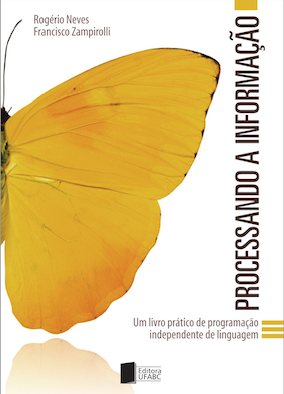
\includegraphics{"figs/Capa_Processando_Informacao.jpg"}

Este caderno (Notebook) é parte complementar \emph{online} do livro
\textbf{\href{https://editora.ufabc.edu.br/matematica-e-ciencias-da-computacao/58-processando-a-informacao}{Processando
a Informação}: um livro prático de programação independente de
linguagem}, que deve ser consultado no caso de dúvidas sobre os temas
apresentados.

\begin{quote}
Este conteúdo pode ser copiado e alterado livremente e foi inspirado
nesse livro.
\end{quote}

    \textbf{Bem vindo ao Google Colab!}

Se você é novo no uso do Colab, assista os vários
\href{https://www.youtube.com/results?search_query=introdu\%C3\%A7\%C3\%A3o+ao+colab}{vídeos
em português} explicando a plataforma. Existem também \textbf{workbooks}
introdutórios para o uso do Python e do Colab na
\href{https://colab.research.google.com/}{página principal} do projeto.

De forma muito resumida, o Colab combina \textbf{células de texto e de
código}. Esse paradigma de juntar documentação e código em um único
documento foi introduzido por Donald Knuth em 1984
{[}\href{https://www-cs-faculty.stanford.edu/~knuth/}{ref1},
\href{http://www.literateprogramming.com}{ref2}{]}.

    \hypertarget{instruuxe7uxf5es}{%
\subsection{Instruções}\label{instruuxe7uxf5es}}

    \begin{itemize}
\tightlist
\item
  É recomendado tirar uma cópia deste notebook clicando em
  \textbf{``Arquivo''}--\textgreater{}\textbf{``Salvar cópia no
  drive''}. Desta forma você poderá editá-lo e executar os campos de
  código sempre que quiser, sem perder os seu progresso ao fechar esta
  página. Essa cópia estará disponível na pasta \textbf{Colab
  Notebooks}, no seu Google Drive.
\item
  Para poder editar uma \textbf{CÉLULA DE TEXTO} (como esta), basta dar
  dois cliques na célula e editar, que pode ser visualizada na aba à
  direita (ou abaixo), ou pressionar Shift+Enter, ou ainda clicando em
  outra célula.
\item
  No Colab também tem a \textbf{CÉLULA DE CÓDIGO}, que pode ser
  executada com essa combinação de teclas, ou clique no botão
  \textbf{``executar''} ou \textbf{``play''} para ver a saída do código
  entrado.
\item
  É recomendado seguir a ordem sugerida dos exercícios, uma vez que
  familiaridade com os conceitos introduzidos são esperados nos
  exercícios seguintes.
\item
  É possível rodar códigos independentes em IDEs e também \emph{online},
  utilizando navegadores, como o Chrome: https://ideone.com/,
  https://www.codechef.com/ide, https://replit.com/,
  https://www.jdoodle.com
\item
  É possível também rodar códigos no seu celular, utilizando navegadores
  acessando esses links.
\item
  Esse arquivo com extensão \texttt{ipynb} pode ser editado também no
  Jupyter Notebook - https://jupyter.org.
\end{itemize}

    \hypertarget{sumuxe1rio}{%
\subsection{Sumário}\label{sumuxe1rio}}

\begin{itemize}
\tightlist
\item
  Introdução à arquitetura de computadores; Hardware e Software
\item
  Algoritmos, fluxogramas e lógica de programação
\item
  Conceitos de linguagens de programação
\item
  Variáveis, tipos de dados e organização da memória
\item
  Operadores e precedência
\item
  Aprendendo a programar
\item
  Revisão deste capítulo
\item
  Exercícios
\end{itemize}

    \hypertarget{introduuxe7uxe3o-uxe0-arquitetura-de-computadores}{%
\subsection{Introdução à Arquitetura de
Computadores}\label{introduuxe7uxe3o-uxe0-arquitetura-de-computadores}}

    A arquitetura (ou organização dos principais componentes) mais conhecida
de computadores foi introduzida por John Von Newmann, em 1936, ver
Figura abaixo.

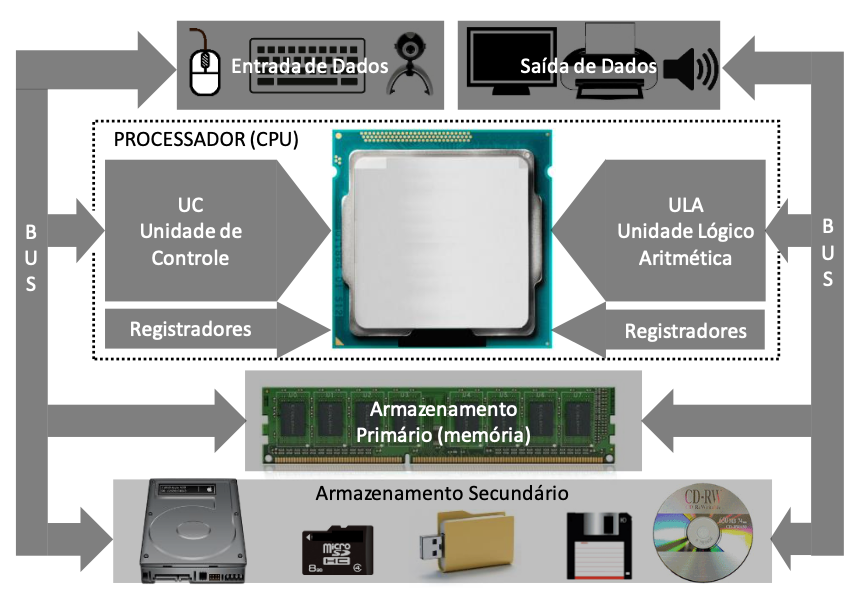
\includegraphics{"figs/image02.png"}

    \begin{figure}
\centering
\caption{Captura de Tela 2021-03-26 às 11.26.59.png}
\end{figure}

    \begin{itemize}
\item
  Um software é um conjunto de linhas de código, armazenado em arquivo
  na memória secundária ou na RAM, que pode ser execudado, instrução por
  instrução na CPU.
\item
  Essas linhas de código são instruções que o computador consegue
  executar, mas que podem ter sido traduzidas de um \textbf{Algoritmo}.
\end{itemize}

    \hypertarget{algoritmos-fluxogramas-e-luxf3gica-de-programauxe7uxe3o}{%
\subsection{Algoritmos, Fluxogramas e Lógica de
Programação}\label{algoritmos-fluxogramas-e-luxf3gica-de-programauxe7uxe3o}}

    \begin{verbatim}
ALGORITMO (algumas definições):
1. Um processo ou conjunto de regras a serem seguidas em cálculo ou outra
operação de solução de problemas, especialmente por um computador.
2. Processo de resolução de um problema constituído por uma sequência 
ordenada e bem definida de passos que, em tempo finito, conduzem à 
solução do problema ou indicam que, para o mesmo, não existem soluções.
\end{verbatim}

    Um exemplo de algoritmo: solução de uma equação do segundo grau no
formato \(ax^2 + bx + c\), dados \(a\), \(b\) e \(c\):

\begin{enumerate}
\def\labelenumi{\arabic{enumi}.}
\tightlist
\item
  Calcule \(\Delta\) com a fórmula \(\Delta = b^2-4ac\);
\item
  Se \(\Delta < 0\), \(x\) não possui raízes reais;
\item
  Se \(\Delta = 0\), \(x\) possui duas raízes reais idênticas;
\item
  Se \(\Delta > 0\), \(x\) possui duas raízes reais e distintas;
\item
  Calcule \(x\) usando a equação.
\end{enumerate}

    \hypertarget{pseudocuxf3digo}{%
\subsubsection{Pseudocódigo}\label{pseudocuxf3digo}}

    \begin{itemize}
\item
  Essa sequência de passos definidas no algoritmo anterior, se incluída
  as instruções \texttt{leia(algo)} e \texttt{escreva(algo)}, poder ser
  definida como um \textbf{pseudocódigo}.
\item
  Esse \textbf{pseudocódigo} é para humanos conseguirem entender os
  passos de um algoritmo, de uma forma ``mais próxima'' de como os
  computadores processam as instruções, utilizando uma linguagem de
  programação, definidas na próxima seção.
\end{itemize}

Veja a seguir um exemplo de pseudocódigo do algoritmo anterior:

    \begin{verbatim}
leia(a,b,c)
calcular delta = b**2-4*a*c
se delta < 0: 
   escreva(x não possui raízes reais)
   fim do programa
se delta = 0:
   escreva(x possui duas raízes reais idênticas)
se delta > 0:
   escreva(x possui duas raízes reais e distintas)
calcule x=a*x*x+b*x+c
escreva(x)
\end{verbatim}

    Observe que em um pseudocódigo existe uma descrição um pouco mais
detalhada das instruções, que em um algoritmo, mas não é uma descrição
muito rígida/formal, como existem nas linguagems de programação.

    \hypertarget{fluxogramas}{%
\subsubsection{Fluxogramas}\label{fluxogramas}}

    \begin{itemize}
\item
  Os algoritmos, além de poderem ser representados por listas de
  instruções, como no último exemplo, podem ser representados
  graficamente para facilitar seu entendimento.
\item
  Os fluxogramas e diagramas de atividades da UML (\emph{Unified
  Modelling Language}) estão entre as representações mais usadas.
\item
  Ambos, bem similares, usam formas e setas para indicar operações e
  seus fluxos.
\item
  A Figura abaixo ilustra um exemplo de fluxograma.
\end{itemize}

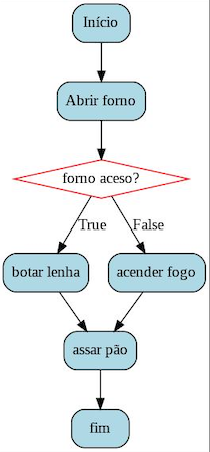
\includegraphics{"figs/flowchart.jpg"}

    \begin{figure}
\centering
\caption{flowchart.jpg}
\end{figure}

    Esse fluxograma foi gerado automaticamente rodando as duas células de
código abaixo.

\textbf{Observação:} apesar do livro texto ser independente de
linguangem, alguns códigos nesta adaptação em Colab serão apresentados
na linguagem de programação Python, pela facilidade didática na
apresentação de conteúdos. Assim, os detalhes desses códigos não serão
apresentados, pois foge o escopo.

    \begin{tcolorbox}[breakable, size=fbox, boxrule=1pt, pad at break*=1mm,colback=cellbackground, colframe=cellborder]
\prompt{In}{incolor}{ }{\boxspacing}
\begin{Verbatim}[commandchars=\\\{\}]
\PY{c+c1}{\PYZsh{} instalando algumas bibliotecas no servidor do Colab (Linux)}
\PY{o}{!}apt\PYZhy{}get install graphviz libgraphviz\PYZhy{}dev pkg\PYZhy{}config
\PY{o}{!}pip install txtoflow
\end{Verbatim}
\end{tcolorbox}

    \begin{tcolorbox}[breakable, size=fbox, boxrule=1pt, pad at break*=1mm,colback=cellbackground, colframe=cellborder]
\prompt{In}{incolor}{ }{\boxspacing}
\begin{Verbatim}[commandchars=\\\{\}]
\PY{c+c1}{\PYZsh{} importando a biblioteca txtflow para gerar fluxograma a partir de código}
\PY{k+kn}{from} \PY{n+nn}{txtoflow} \PY{k+kn}{import} \PY{n}{txtoflow}

\PY{c+c1}{\PYZsh{} definindo o pseudocódigo e passando como entrada de dados para gerar o fluxograma}
\PY{n}{txtoflow}\PY{o}{.}\PY{n}{generate}\PY{p}{(}
    \PY{l+s+sd}{\PYZsq{}\PYZsq{}\PYZsq{}}
\PY{l+s+sd}{    Início;}
\PY{l+s+sd}{    Abrir forno;}
\PY{l+s+sd}{    if (forno aceso?) \PYZob{}}
\PY{l+s+sd}{        botar lenha;}
\PY{l+s+sd}{    \PYZcb{} else \PYZob{}}
\PY{l+s+sd}{        acender fogo;}
\PY{l+s+sd}{    \PYZcb{}}
\PY{l+s+sd}{    assar pão;}
\PY{l+s+sd}{    fim;}
\PY{l+s+sd}{    \PYZsq{}\PYZsq{}\PYZsq{}}
\PY{p}{)}
\end{Verbatim}
\end{tcolorbox}

    \begin{itemize}
\tightlist
\item
  Após rodar a célula de código acima, ver o arquivo
  \texttt{flowchart.jpg} clicando no ícone de pasta à esquerda.
\end{itemize}

    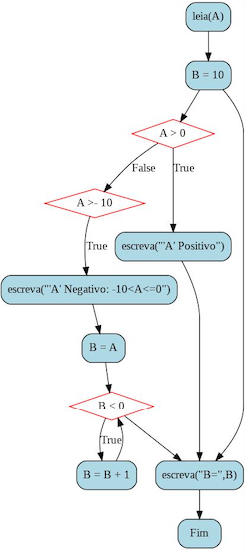
\includegraphics{"figs/flowchart2.jpg"}

\begin{itemize}
\tightlist
\item
  Veja um outro fluxograma gerado a partir da célula abaixo;
  \textgreater{} Apesar deste primeiro fluxograma ser intuitivo, os
  detalhes (principalmente do próximo fluxograma) serão vistos durantes
  este curso!
\end{itemize}

    \begin{tcolorbox}[breakable, size=fbox, boxrule=1pt, pad at break*=1mm,colback=cellbackground, colframe=cellborder]
\prompt{In}{incolor}{ }{\boxspacing}
\begin{Verbatim}[commandchars=\\\{\}]
\PY{c+c1}{\PYZsh{} definindo uma variável do tipo texto (string) para armazenar o pseudocódigo}
\PY{n}{alg2} \PY{o}{=} \PY{l+s+s1}{\PYZsq{}\PYZsq{}\PYZsq{}}
\PY{l+s+s1}{leia(A);}
\PY{l+s+s1}{B = 10;}
\PY{l+s+s1}{if ( A \PYZgt{} 0 ) }\PY{l+s+s1}{\PYZob{}}
\PY{l+s+s1}{  escreva(}\PY{l+s+s1}{\PYZdq{}}\PY{l+s+s1}{\PYZsq{}}\PY{l+s+s1}{A}\PY{l+s+s1}{\PYZsq{}}\PY{l+s+s1}{ Positivo}\PY{l+s+s1}{\PYZdq{}}\PY{l+s+s1}{);}
\PY{l+s+s1}{\PYZcb{} else if ( A \PYZgt{}\PYZhy{} 10 ) }\PY{l+s+s1}{\PYZob{}}
\PY{l+s+s1}{  escreva(}\PY{l+s+s1}{\PYZdq{}}\PY{l+s+s1}{\PYZsq{}}\PY{l+s+s1}{A}\PY{l+s+s1}{\PYZsq{}}\PY{l+s+s1}{ Negativo: \PYZhy{}10\PYZlt{}A\PYZlt{}=0}\PY{l+s+s1}{\PYZdq{}}\PY{l+s+s1}{);}
\PY{l+s+s1}{  B = A;}
\PY{l+s+s1}{  while ( B \PYZlt{} 0 ) }\PY{l+s+s1}{\PYZob{}}
\PY{l+s+s1}{    B = B + 1;}
\PY{l+s+s1}{  \PYZcb{}}
\PY{l+s+s1}{\PYZcb{}}
\PY{l+s+s1}{escreva(}\PY{l+s+s1}{\PYZdq{}}\PY{l+s+s1}{B=}\PY{l+s+s1}{\PYZdq{}}\PY{l+s+s1}{,B);}
\PY{l+s+s1}{Fim;}\PY{l+s+s1}{\PYZsq{}\PYZsq{}\PYZsq{}}

\PY{c+c1}{\PYZsh{} criando o fluxograma}
\PY{n}{txtoflow}\PY{o}{.}\PY{n}{generate}\PY{p}{(}\PY{n}{alg2}\PY{p}{)}
\end{Verbatim}
\end{tcolorbox}

    \begin{figure}
\centering
\caption{flowchart2.jpg}
\end{figure}

    \begin{itemize}
\tightlist
\item
  Qual o valor final de B neste algoritmo, se o valor lido foi
  \texttt{A=-5}?
\item
  Experimente também essa ferramenta \emph{online}:
  \href{https://app.code2flow.com/}{code2flow}
\end{itemize}

    \hypertarget{fluxograma-a-partir-de-cuxf3digo-python}{%
\paragraph{Fluxograma a partir de código
python}\label{fluxograma-a-partir-de-cuxf3digo-python}}

    A sequência de códigos a seguir geram fluxogramas na própria célula de
código, diferente de salvar em arquivo de imagem. Além disso, a entrada
é um código em python, diferente do exemplo anterior que está em
pseudocódigo.

    \begin{tcolorbox}[breakable, size=fbox, boxrule=1pt, pad at break*=1mm,colback=cellbackground, colframe=cellborder]
\prompt{In}{incolor}{ }{\boxspacing}
\begin{Verbatim}[commandchars=\\\{\}]
\PY{o}{!}pip install \PYZhy{}\PYZhy{}upgrade git+https://github.com/innovationOUtside/flowchart\PYZus{}js\PYZus{}jp\PYZus{}proxy\PYZus{}widget.git
\end{Verbatim}
\end{tcolorbox}

    \begin{tcolorbox}[breakable, size=fbox, boxrule=1pt, pad at break*=1mm,colback=cellbackground, colframe=cellborder]
\prompt{In}{incolor}{ }{\boxspacing}
\begin{Verbatim}[commandchars=\\\{\}]
\PY{k+kn}{from} \PY{n+nn}{google}\PY{n+nn}{.}\PY{n+nn}{colab} \PY{k+kn}{import} \PY{n}{output}
\PY{n}{output}\PY{o}{.}\PY{n}{enable\PYZus{}custom\PYZus{}widget\PYZus{}manager}\PY{p}{(}\PY{p}{)}
\end{Verbatim}
\end{tcolorbox}

    \begin{tcolorbox}[breakable, size=fbox, boxrule=1pt, pad at break*=1mm,colback=cellbackground, colframe=cellborder]
\prompt{In}{incolor}{ }{\boxspacing}
\begin{Verbatim}[commandchars=\\\{\}]
\PY{n}{alg3} \PY{o}{=} \PY{l+s+s1}{\PYZsq{}\PYZsq{}\PYZsq{}}
\PY{l+s+s1}{A = int(input())}
\PY{l+s+s1}{B = 10}
\PY{l+s+s1}{if A \PYZgt{} 0:}
\PY{l+s+s1}{  print(}\PY{l+s+s1}{\PYZdq{}}\PY{l+s+s1}{\PYZsq{}}\PY{l+s+s1}{A}\PY{l+s+s1}{\PYZsq{}}\PY{l+s+s1}{ Positivo}\PY{l+s+s1}{\PYZdq{}}\PY{l+s+s1}{)}
\PY{l+s+s1}{elif A \PYZgt{} \PYZhy{}10:}
\PY{l+s+s1}{  print(}\PY{l+s+s1}{\PYZdq{}}\PY{l+s+s1}{\PYZsq{}}\PY{l+s+s1}{A}\PY{l+s+s1}{\PYZsq{}}\PY{l+s+s1}{ Negativo: \PYZhy{}10\PYZlt{}A\PYZlt{}=0}\PY{l+s+s1}{\PYZdq{}}\PY{l+s+s1}{)}
\PY{l+s+s1}{  B = A}
\PY{l+s+s1}{  while B \PYZlt{} 0:}
\PY{l+s+s1}{    B = B + 1}
\PY{l+s+s1}{    print(B)}
\PY{l+s+s1}{print(}\PY{l+s+s1}{\PYZdq{}}\PY{l+s+s1}{B=}\PY{l+s+s1}{\PYZdq{}}\PY{l+s+s1}{,B)}\PY{l+s+s1}{\PYZsq{}\PYZsq{}\PYZsq{}}
\end{Verbatim}
\end{tcolorbox}

    \begin{tcolorbox}[breakable, size=fbox, boxrule=1pt, pad at break*=1mm,colback=cellbackground, colframe=cellborder]
\prompt{In}{incolor}{ }{\boxspacing}
\begin{Verbatim}[commandchars=\\\{\}]
\PY{k+kn}{from} \PY{n+nn}{pyflowchart} \PY{k+kn}{import} \PY{n}{Flowchart}
\PY{n}{fc} \PY{o}{=} \PY{n}{Flowchart}\PY{o}{.}\PY{n}{from\PYZus{}code}\PY{p}{(}\PY{n}{alg3}\PY{p}{)}
\PY{n}{flowchart} \PY{o}{=} \PY{n}{fc}\PY{o}{.}\PY{n}{flowchart}\PY{p}{(}\PY{p}{)}
\end{Verbatim}
\end{tcolorbox}

    \begin{tcolorbox}[breakable, size=fbox, boxrule=1pt, pad at break*=1mm,colback=cellbackground, colframe=cellborder]
\prompt{In}{incolor}{ }{\boxspacing}
\begin{Verbatim}[commandchars=\\\{\}]
\PY{k+kn}{from} \PY{n+nn}{jp\PYZus{}flowchartjs}\PY{n+nn}{.}\PY{n+nn}{jp\PYZus{}flowchartjs} \PY{k+kn}{import} \PY{n}{FlowchartWidget}

\PY{n}{testEmbed} \PY{o}{=} \PY{n}{FlowchartWidget}\PY{p}{(}\PY{p}{)}
\PY{n}{testEmbed}\PY{o}{.}\PY{n}{charter}\PY{p}{(}\PY{n}{flowchart}\PY{p}{)}
\PY{n}{testEmbed}
\end{Verbatim}
\end{tcolorbox}

    \begin{itemize}
\item
  Comparando os dois fluxogramas anteriores é possível notar que é mais
  difícil ler esse último por falta de cor e por ter cruzamentos entre
  retas.
\item
  Achou alguma ferramenta mais interessante para gerar fluxograma neste
  Colab? Compartilhe!

  \begin{itemize}
  \tightlist
  \item
    Por exemplo, seria interessante criar um fluxograma a partir de uma
    célula de código, contendo várias instruções, e não a partir de um
    texto, como ocorre na ferramenta \emph{online} anterior.
  \end{itemize}
\end{itemize}

    \hypertarget{conceitos-de-linguagens-de-programauxe7uxe3o}{%
\subsection{Conceitos de Linguagens de
Programação}\label{conceitos-de-linguagens-de-programauxe7uxe3o}}

    Linguagem é um conjunto de regras usado para se definir uma forma de
comunicação. São conceitos fundamentais de qualquer linguagem, não só em
computação:

\begin{itemize}
\tightlist
\item
  \textbf{sintaxe:} o arranjo de palavras e sua disposição em um
  discurso para criar frases bem formadas e relacionadas de forma lógica
  em uma linguagem;
\item
  \textbf{semântica:} o ramo da linguística preocupado com a lógica e o
  significado das palavras. sub-ramos incluem a semântica formal e a
  semântica lexical.
\end{itemize}

    \hypertarget{nuxedveis-de-liguagens}{%
\subsubsection{Níveis de Liguagens}\label{nuxedveis-de-liguagens}}

    Nível de linguagem diz respeito à proximidade em que ela se encontra da
linguagem natural humana.

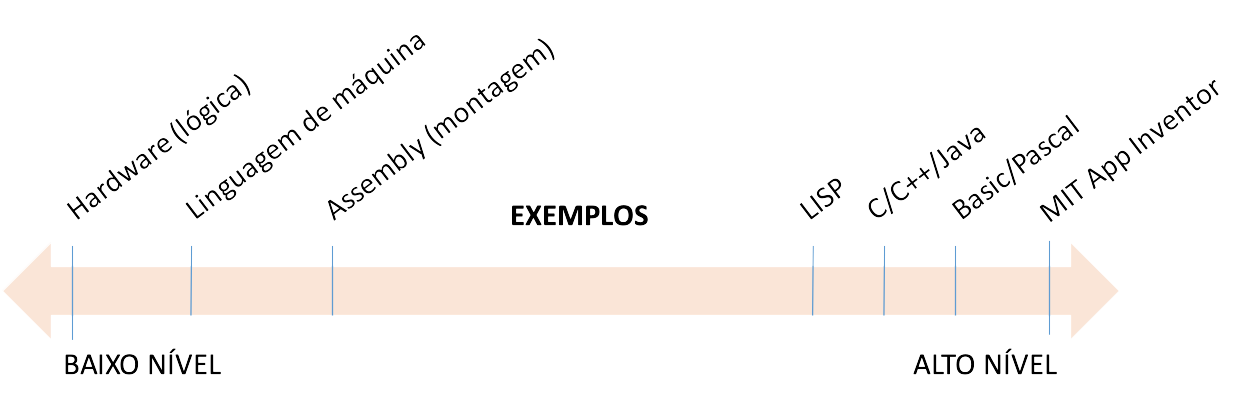
\includegraphics{"figs/image03.png"}

    \begin{figure}
\centering
\caption{image.png}
\end{figure}

    \hypertarget{linguagem-compilada-vs-interpretada}{%
\subsubsection{Linguagem Compilada vs
Interpretada}\label{linguagem-compilada-vs-interpretada}}

    \begin{itemize}
\item
  A \textbf{compilação} é o nome dado ao processo de traduzir um código
  escrito em uma linguagem de mais alto-nível para código de máquina,
  que poderá ser executado na arquitetura apropriada para o qual foi
  compilado.

  \begin{itemize}
  \tightlist
  \item
    Exemplos de linguagens compiladas: C, CPP (ou C++), Pascal e
    Fortran.
  \end{itemize}
\item
  Em \textbf{linguagens interpretadas}, os comandos do programa são
  transformados em código nativo durante a sua execução, geralmente por
  um outro programa, necessário para seu funcionamento.

  \begin{itemize}
  \tightlist
  \item
    Exemplos de linguagens interpretadas: python (nesse Colab), R,
    matlab.
  \end{itemize}
\item
  A exceção é a linguagem \textbf{Java}, que compila um código binário
  em bytes (\textbf{bytecode}), para ser executado não em uma
  arquitetura real específica, mas sim pela \textbf{máquina virtual
  Java} (JVM), que é um \textbf{programa nativo} (isto é, é necessário
  um JVM compilado para cada arquitetura) responsável por transformar
  \emph{bytecode} na linguagem de máquina nativa do processador em tempo
  de execução (\textbf{runtime}).
\item
  A existência de JVM para a maioria das plataformas aumentou em muito a
  portabilidade dos programas. A \textbf{portabilidade} foi uma das
  principais motivações para a criação da linguagem Java.
\end{itemize}

    \hypertarget{estruturas-de-cuxf3digo}{%
\subsubsection{Estruturas de Código}\label{estruturas-de-cuxf3digo}}

    Independente da linguagem escolhida, as estruturas fundamentais de
código que estarão presentes em todas elas são:

\begin{enumerate}
\def\labelenumi{\arabic{enumi}.}
\tightlist
\item
  \textbf{Código sequencial:} os comandos são executados na ordem em que
  aparecem;
\item
  \textbf{Módulos de código (funções ou métodos):} conjuntos de comandos
  agrupados em sub-rotinas ou subprogramas;
\item
  \textbf{Desvios condicionais:} dada uma condição, existem dois
  caminhos possíveis (duas linhas) de execução;
\item
  \textbf{Estruturas de repetição ou laços:} conjuntos de comandos que
  se repetem enquanto uma dada condição for satisfeita.
\end{enumerate}

    \hypertarget{deburauxe7uxe3o-de-cuxf3digo-debug}{%
\subsubsection{Deburação de Código
(DEBUG)}\label{deburauxe7uxe3o-de-cuxf3digo-debug}}

    \begin{itemize}
\item
  É referido como depuração ou ``debugação'' o árduo processo de busca e
  correção dos erros de programação no código escrito em linguagens de
  programação.
\item
  Ferramentas de depuração são de grande valia para auxiliar na busca e
  correção destes erros.
\item
  Alguns dos erros comuns encontrados em código, do menos grave ao mais
  sério, são:
\end{itemize}

    \begin{quote}
\begin{enumerate}
\def\labelenumi{\arabic{enumi}.}
\tightlist
\item
  \textbf{Erro de semântica:} palavras reservadas ou operações escritas
  de forma errada;
\item
  \textbf{Erro de sintaxe:} envolve o uso inapropriado do formato dos
  comandos;
\item
  \textbf{Erro de organização:} blocos de código, aspas ou uso de
  parênteses inconsistentes -- ocorre quando se abre um bloco de código
  ou de operadores (com chaves, colchetes ou parênteses) ou um campo de
  texto (com aspas) sem fechar ou se fecha sem abrir;
\item
  \textbf{Erro de lógica:} também conhecido como \emph{Cerberus} (o cão
  de guarda do inferno), ocorre quando os comandos estão sintaticamente
  corretos, na semântica correta, e escritos consistentemente, porém em
  ordem, forma ou disposição que produz um resultado diferente do
  desejado. Resultado este que, frequentemente, causa travamento da
  execução do programa ou até mesmo do computador.
\end{enumerate}
\end{quote}

    \hypertarget{ambientes-de-desenvolvimento-integrados}{%
\subsubsection{Ambientes de Desenvolvimento
Integrados}\label{ambientes-de-desenvolvimento-integrados}}

    Ambientes de desenvolvimento integrado ou IDE (\emph{Integrated
Developing Environment}), como são conhecidos, oferecem uma combinação
de ferramentas úteis para escrita, execução e depuração do código de
programas.

    Algumas ferramentas de desenvolvimento populares do tipo IDE são: -
\textbf{Eclipse} (C, CPP, Java, PHP, android, etc); - \textbf{NetBeans}
(C, CPP, Java, ruby, HTMl5, PHP, etc); - \textbf{PyCharm} (Python,
JavaScript, CoffeeScript, XML, HTML/XHTML); - \textbf{Xcode} (IDE de
desenvolvimento para dispositivos Apple); - \textbf{Visual studio} (C,
CPP, C\#, visual Basic, entre outros, voltado para o desenvolvimento de
programas na plataforma Windows). -
\textbf{\href{https://vscode.dev}{VSCODE}} (versão \emph{online} de
código aberto do \emph{Visual studio}. Para download e uso local:
https://code.visualstudio.com/download).

    Mais alguns links úteis para programar em várias linguagens
\emph{online}:

\begin{itemize}
\item
  https://colab.research.google.com
\item
  https://replit.com/languages
\item
  http://www.drjava.org
\item
  https://sourceforge.net/projects/nbportable
\item
  https://ideone.com
\item
  https://www.codechef.com/ide

  Python:
\item
  https://www.programiz.com/python-programming/online-compiler/
\item
  https://www.onlinegdb.com/online\_python\_compiler
\item
  https://www.tutorialspoint.com/execute\_python\_online.php
\item
  https://www.python.org/shell/
\item
  http://pythontutor.com
\end{itemize}

Ou para Baixar IDE's: * https://www.anaconda.com/distribution *
https://netbeans.org

Mais links interessantes: * https://learnxinyminutes.com/docs/python3 *
https://learnxinyminutes.com/docs/java *
https://learnxinyminutes.com/docs/c * https://youtu.be/UNSoPa-XQN0

Tem outros links interessantes que não estão nestas listas? Compartilhe!

    \hypertarget{algumas-estatuxedsticas-sobre-linguagens-mais-usadas}{%
\paragraph{Algumas Estatísticas sobre Linguagens Mais
Usadas:}\label{algumas-estatuxedsticas-sobre-linguagens-mais-usadas}}

\begin{itemize}
\tightlist
\item
  https://insights.stackoverflow.com/trends?tags=python\%2Cjava\%2Cjavascript\\
\item
  \href{https://profdanielbrandao.wordpress.com/2019/03/01/o-incrivel-crescimento-da-linguagem-python/}{reportagem}
\item
  https://insights.stackoverflow.com/survey/2020
\item
  https://insights.stackoverflow.com/survey/2020\#most-popular-technologies
\end{itemize}

    \hypertarget{variuxe1veis}{%
\subsection{Variáveis}\label{variuxe1veis}}

    \begin{itemize}
\tightlist
\item
  Uma variável em programação de computadores é um indicador ou
  `apelido' (\emph{alias}) atribuído a um endereço de memória que contém
  um dado guardado.
\item
  Os elementos na memória, representados por variáveis, podem conter
  apenas um ou múltiplos valores, e são codificados na memória de acordo
  com o tipo específico do dado, com formato e número de bits apropriado
  para mantê-los.
\end{itemize}

    \hypertarget{uso-de-variuxe1veis}{%
\subsubsection{Uso de Variáveis}\label{uso-de-variuxe1veis}}

    Em qualquer linguagem, um valor pode ser atribuído a uma variável
através do operador de atribuição, por exemplo: ``\texttt{=}''.

    \hypertarget{exemplos-de-variuxe1veis-do-tipo-inteiro}{%
\paragraph{Exemplos de variáveis do tipo
inteiro:}\label{exemplos-de-variuxe1veis-do-tipo-inteiro}}

    \begin{itemize}
\item
  As próximas células de código em Python podem ser executadas clicando
  em \texttt{{[}\ {]}} ou seta de \emph{play}, na margem esquerda.
\item
  Se o seu objetivo é aprender outras linguagens de programação, essas
  células em Python podem ser utilizadas como comparativos.
\end{itemize}

    \begin{tcolorbox}[breakable, size=fbox, boxrule=1pt, pad at break*=1mm,colback=cellbackground, colframe=cellborder]
\prompt{In}{incolor}{ }{\boxspacing}
\begin{Verbatim}[commandchars=\\\{\}]
\PY{n}{idade} \PY{o}{=} \PY{l+m+mi}{20}\PY{p}{;}     \PY{c+c1}{\PYZsh{} esse é um comentário}
\PY{n}{anoAtual} \PY{o}{=} \PY{l+m+mi}{2021} \PY{c+c1}{\PYZsh{} observer que \PYZsq{};\PYZsq{} é opcional em python e javascript}
\end{Verbatim}
\end{tcolorbox}

    A leitura correta para o código representado acima é \textbf{``a
variável \texttt{idade} recebe o valor 20''}.

    \begin{tcolorbox}[breakable, size=fbox, boxrule=1pt, pad at break*=1mm,colback=cellbackground, colframe=cellborder]
\prompt{In}{incolor}{ }{\boxspacing}
\begin{Verbatim}[commandchars=\\\{\}]
\PY{n}{idade}
\end{Verbatim}
\end{tcolorbox}

    \begin{tcolorbox}[breakable, size=fbox, boxrule=1pt, pad at break*=1mm,colback=cellbackground, colframe=cellborder]
\prompt{In}{incolor}{ }{\boxspacing}
\begin{Verbatim}[commandchars=\\\{\}]
\PY{n}{anoNascimento} \PY{o}{=} \PY{n}{anoAtual} \PY{o}{\PYZhy{}} \PY{n}{idade}
\PY{n}{anoNascimento}
\end{Verbatim}
\end{tcolorbox}

    \hypertarget{exemplo-de-variuxe1vel-do-tipo-texto-string}{%
\paragraph{\texorpdfstring{Exemplo de variável do tipo texto
(\emph{string})}{Exemplo de variável do tipo texto (string)}}\label{exemplo-de-variuxe1vel-do-tipo-texto-string}}

    \begin{tcolorbox}[breakable, size=fbox, boxrule=1pt, pad at break*=1mm,colback=cellbackground, colframe=cellborder]
\prompt{In}{incolor}{ }{\boxspacing}
\begin{Verbatim}[commandchars=\\\{\}]
\PY{n}{nomeAluno} \PY{o}{=} \PY{l+s+s1}{\PYZsq{}}\PY{l+s+s1}{Rafael Morais}\PY{l+s+s1}{\PYZsq{}}
\PY{n}{nomeAluno}
\end{Verbatim}
\end{tcolorbox}

    \begin{tcolorbox}[breakable, size=fbox, boxrule=1pt, pad at break*=1mm,colback=cellbackground, colframe=cellborder]
\prompt{In}{incolor}{ }{\boxspacing}
\begin{Verbatim}[commandchars=\\\{\}]
\PY{n}{nomeAluno} \PY{o}{=} \PY{l+s+s2}{\PYZdq{}}\PY{l+s+s2}{Rafael Morais}\PY{l+s+s2}{\PYZdq{}}
\PY{n}{nomeAluno}
\end{Verbatim}
\end{tcolorbox}

    Observe que o texto deve ficar entre aspas simples ou duplas (dependendo
das linguagem escolhida).

    \hypertarget{exemplo-de-variuxe1vel-do-tipo-real}{%
\paragraph{Exemplo de variável do tipo
real}\label{exemplo-de-variuxe1vel-do-tipo-real}}

    \begin{tcolorbox}[breakable, size=fbox, boxrule=1pt, pad at break*=1mm,colback=cellbackground, colframe=cellborder]
\prompt{In}{incolor}{ }{\boxspacing}
\begin{Verbatim}[commandchars=\\\{\}]
\PY{n}{pi} \PY{o}{=} \PY{l+m+mf}{3.1415926535897932}
\PY{n}{pi}
\end{Verbatim}
\end{tcolorbox}

    Observe que tem que usar `.' para separar as casas decimais.

    \hypertarget{nomenclatura}{%
\paragraph{Nomenclatura}\label{nomenclatura}}

    \begin{itemize}
\item
  Os nomes das variáveis podem conter letras, números e alguns
  caracteres especiais, desde que não sejam empregados pelo lexema da
  linguagem (símbolos dos operadores matemáticos, lógicos e relacionais,
  por exemplo).
\item
  Em geral, o nome da variável deve começar por uma letra ou, dependendo
  da linguagem, algum caractere especial.
\item
  Como regra geral os nomes de variáveis não devem começar com números
  ou conter espaços.
\end{itemize}

    Exemplos de variáveis válidas e inválidas:

\begin{longtable}[]{@{}ll@{}}
\toprule
Válido & Inválido\tabularnewline
\midrule
\endhead
idade4 & 4idade\tabularnewline
Nome\_Completo & Nome Completo\tabularnewline
resta\_um & resta-um\tabularnewline
V8S9F0D7S7D9 & V@R!V\&+\tabularnewline
\bottomrule
\end{longtable}

    \hypertarget{operadores-e-preceduxeancia}{%
\subsection{Operadores e
precedência}\label{operadores-e-preceduxeancia}}

    As linguagens reservam alguns caracteres para uso em operadores ou
indicadores de tipo.

    \hypertarget{operadores-aritmeticos}{%
\subsubsection{Operadores aritmeticos}\label{operadores-aritmeticos}}

    **

Tabela: Operadores aritméticos em Java/C/CPP/JS

**

\begin{longtable}[]{@{}ll@{}}
\toprule
operador & descrição\tabularnewline
\midrule
\endhead
+ & soma com\tabularnewline
- & subtração por\tabularnewline
* & multiplicação por\tabularnewline
/ & divisão por\tabularnewline
\% & resto da divisão por\tabularnewline
++ & incremento\tabularnewline
-- & decremento\tabularnewline
\bottomrule
\end{longtable}

    \hypertarget{operadores-relacionais}{%
\subsubsection{Operadores relacionais}\label{operadores-relacionais}}

    **

Tabela: Operadores relacionais em Java/C/CPP/JS

**

\begin{longtable}[]{@{}ll@{}}
\toprule
operador & descrição\tabularnewline
\midrule
\endhead
== & é igual a\tabularnewline
!= & é diferente de\tabularnewline
\textgreater{} & é maior que\tabularnewline
\textless{} & é menor que\tabularnewline
\textgreater= & é maior ou igual a\tabularnewline
\textless= & é menor ou igual a\tabularnewline
\bottomrule
\end{longtable}

    \hypertarget{operadores-luxf3gicos}{%
\subsubsection{Operadores lógicos}\label{operadores-luxf3gicos}}

    **

Tabela: Operadores lógicos binários em Java/C/CPP/JS

**

\begin{longtable}[]{@{}ll@{}}
\toprule
operador & descrição\tabularnewline
\midrule
\endhead
x \textbf{\&\&} y & True se ambos também forem\tabularnewline
x \textbf{\&} y & True se ambos também forem bit-a-bit\tabularnewline
x \textbf{\textbar\textbar{}} y & False se ambos também
forem\tabularnewline
x \textbf{\textbar{}} y & False se ambos também forem
bit-a-bit\tabularnewline
\textbf{!} x & contrário de x\tabularnewline
\textbf{\textasciitilde{}} x & contrário de x bit-a-bit\tabularnewline
\textbf{\^{}} x & ou exclusivo \texttt{XOR} bit-a-bit\tabularnewline
\textbf{\textless\textless{}}N & \emph{shift-left}, adiciona N zeros à
direita do número binário\tabularnewline
\textbf{\textless\textless{}}N & \emph{shift-right}, elimina N zeros à
direita do número binário\tabularnewline
\bottomrule
\end{longtable}

    \hypertarget{operadores-de-atribuiuxe7uxe3o}{%
\subsubsection{Operadores de
atribuição}\label{operadores-de-atribuiuxe7uxe3o}}

    **

Tabela: Operadores de atribuição em Python/Java/C/CPP/JS

**

\begin{longtable}[]{@{}ll@{}}
\toprule
operador & descrição\tabularnewline
\midrule
\endhead
= & recebe o valor de\tabularnewline
+= & é somado ao valor de\tabularnewline
-= & é subtraído do valor de\tabularnewline
*= & é multiplicado pelo valor de\tabularnewline
/= & é dividido pelo valor de\tabularnewline
\%= & recebe o resto da divisão por\tabularnewline
similarmente & \textgreater\textgreater=, \textless\textless=,
\&=,\tabularnewline
\bottomrule
\end{longtable}

    \begin{center}\rule{0.5\linewidth}{0.5pt}\end{center}

    \hypertarget{preceduxeancia-de-operadores}{%
\subsubsection{Precedência de
Operadores}\label{preceduxeancia-de-operadores}}

    Quando utilizados em uma expressão, os operadores apresentados
anteriormente são executados em ordem de precedência, de forma
semelhante como fazemos em equações matemáticas, com somas, subtrações,
multiplicações, divisões, exponenciais, etc. (testar Tabela abaixo na
linguagem escolhida).

    **

Tabela: Precedência de Operadores

**

\begin{longtable}[]{@{}lll@{}}
\toprule
\begin{minipage}[b]{0.26\columnwidth}\raggedright
Categoria\strut
\end{minipage} & \begin{minipage}[b]{0.44\columnwidth}\raggedright
Operador\strut
\end{minipage} & \begin{minipage}[b]{0.21\columnwidth}\raggedright
Associatividade\strut
\end{minipage}\tabularnewline
\midrule
\endhead
\begin{minipage}[t]{0.26\columnwidth}\raggedright
Pós-fixado\strut
\end{minipage} & \begin{minipage}[t]{0.44\columnwidth}\raggedright
() (parênteses, operador ponto)\strut
\end{minipage} & \begin{minipage}[t]{0.21\columnwidth}\raggedright
\(\rightarrow\) Esquerda para a direita\strut
\end{minipage}\tabularnewline
\begin{minipage}[t]{0.26\columnwidth}\raggedright
Índice\strut
\end{minipage} & \begin{minipage}[t]{0.44\columnwidth}\raggedright
{[}{]}\strut
\end{minipage} & \begin{minipage}[t]{0.21\columnwidth}\raggedright
\(\rightarrow\) Esquerda para a direita\strut
\end{minipage}\tabularnewline
\begin{minipage}[t]{0.26\columnwidth}\raggedright
Unário\strut
\end{minipage} & \begin{minipage}[t]{0.44\columnwidth}\raggedright
++ - - ! \textasciitilde{} (incremento, decremento)\strut
\end{minipage} & \begin{minipage}[t]{0.21\columnwidth}\raggedright
\(\leftarrow\) Direita para a esquerda\strut
\end{minipage}\tabularnewline
\begin{minipage}[t]{0.26\columnwidth}\raggedright
Multiplicativo\strut
\end{minipage} & \begin{minipage}[t]{0.44\columnwidth}\raggedright
* / \% (vezes, dividido, resto)\strut
\end{minipage} & \begin{minipage}[t]{0.21\columnwidth}\raggedright
\(\rightarrow\) Esquerda para a direita\strut
\end{minipage}\tabularnewline
\begin{minipage}[t]{0.26\columnwidth}\raggedright
Aditivo\strut
\end{minipage} & \begin{minipage}[t]{0.44\columnwidth}\raggedright
+ - (soma, subtração)\strut
\end{minipage} & \begin{minipage}[t]{0.21\columnwidth}\raggedright
\(\rightarrow\) Esquerda para a direita\strut
\end{minipage}\tabularnewline
\begin{minipage}[t]{0.26\columnwidth}\raggedright
Shift binário\strut
\end{minipage} & \begin{minipage}[t]{0.44\columnwidth}\raggedright
\textgreater\textgreater{} \textgreater\textgreater\textgreater{}
\textless\textless{}\strut
\end{minipage} & \begin{minipage}[t]{0.21\columnwidth}\raggedright
\(\rightarrow\) Esquerda para a direita\strut
\end{minipage}\tabularnewline
\begin{minipage}[t]{0.26\columnwidth}\raggedright
Relacional\strut
\end{minipage} & \begin{minipage}[t]{0.44\columnwidth}\raggedright
\textgreater{} \textgreater= \textless{} \textless=\strut
\end{minipage} & \begin{minipage}[t]{0.21\columnwidth}\raggedright
\(\rightarrow\) Esquerda para a direita\strut
\end{minipage}\tabularnewline
\begin{minipage}[t]{0.26\columnwidth}\raggedright
Igualdade\strut
\end{minipage} & \begin{minipage}[t]{0.44\columnwidth}\raggedright
== != (é igual a, é diferente de)\strut
\end{minipage} & \begin{minipage}[t]{0.21\columnwidth}\raggedright
\(\rightarrow\) Esquerda para a direita\strut
\end{minipage}\tabularnewline
\begin{minipage}[t]{0.26\columnwidth}\raggedright
E (AND) bit-a-bit\strut
\end{minipage} & \begin{minipage}[t]{0.44\columnwidth}\raggedright
\&\strut
\end{minipage} & \begin{minipage}[t]{0.21\columnwidth}\raggedright
\(\rightarrow\) Esquerda para a direita\strut
\end{minipage}\tabularnewline
\begin{minipage}[t]{0.26\columnwidth}\raggedright
XOR bit-a-bit\strut
\end{minipage} & \begin{minipage}[t]{0.44\columnwidth}\raggedright
\^{}\strut
\end{minipage} & \begin{minipage}[t]{0.21\columnwidth}\raggedright
\(\rightarrow\) Esquerda para a direita\strut
\end{minipage}\tabularnewline
\begin{minipage}[t]{0.26\columnwidth}\raggedright
Ou (OR) bit-a-bit\strut
\end{minipage} & \begin{minipage}[t]{0.44\columnwidth}\raggedright
\textbar{}\strut
\end{minipage} & \begin{minipage}[t]{0.21\columnwidth}\raggedright
\(\rightarrow\) Esquerda para a direita\strut
\end{minipage}\tabularnewline
\begin{minipage}[t]{0.26\columnwidth}\raggedright
E lógico\strut
\end{minipage} & \begin{minipage}[t]{0.44\columnwidth}\raggedright
\&\&\strut
\end{minipage} & \begin{minipage}[t]{0.21\columnwidth}\raggedright
\(\rightarrow\) Esquerda para a direita\strut
\end{minipage}\tabularnewline
\begin{minipage}[t]{0.26\columnwidth}\raggedright
Ou lógico\strut
\end{minipage} & \begin{minipage}[t]{0.44\columnwidth}\raggedright
\textbar\textbar{}\strut
\end{minipage} & \begin{minipage}[t]{0.21\columnwidth}\raggedright
\(\rightarrow\) Esquerda para a direita\strut
\end{minipage}\tabularnewline
\begin{minipage}[t]{0.26\columnwidth}\raggedright
Condicional\strut
\end{minipage} & \begin{minipage}[t]{0.44\columnwidth}\raggedright
?:\strut
\end{minipage} & \begin{minipage}[t]{0.21\columnwidth}\raggedright
\(\leftarrow\) Direita para a esquerda\strut
\end{minipage}\tabularnewline
\begin{minipage}[t]{0.26\columnwidth}\raggedright
Atribuição\strut
\end{minipage} & \begin{minipage}[t]{0.44\columnwidth}\raggedright
= += -= *= /= \%= \textgreater\textgreater= \textless\textless= \&=
\^{}= \textbar=\strut
\end{minipage} & \begin{minipage}[t]{0.21\columnwidth}\raggedright
\(\leftarrow\) Direita para a esquerda\strut
\end{minipage}\tabularnewline
\bottomrule
\end{longtable}

    \hypertarget{tipos-buxe1sicos-de-variuxe1veis}{%
\paragraph{Tipos básicos de
variáveis}\label{tipos-buxe1sicos-de-variuxe1veis}}

    \hypertarget{conversuxf5es-de-tipos-de-variuxe1veis}{%
\paragraph{Conversões de tipos de
variáveis}\label{conversuxf5es-de-tipos-de-variuxe1veis}}

    **

Tabela: Tipos de variáveis em Java/C/CPP/JS

**

\begin{longtable}[]{@{}lllll@{}}
\toprule
\endhead
\textbf{Tipo} & \textbf{Descrição} & \textbf{n.~Bits} & \textbf{Mínimo}
& \textbf{Máximo ( valor )}\tabularnewline
& & & &\tabularnewline
\textbf{Tipos inteiros+sinal} & & & &\tabularnewline
byte & inteiro de 1 byte & \(8\) & \(-128\) & \(127\)\tabularnewline
short & inteiro curto & \(16\) & \(-2^{15}\) &
\(2^{15}-1\)\tabularnewline
int & inteiro & \(32\) & \(-2^{31}\) & \(2^{31}-1\)\tabularnewline
long & inteiro longo & \(64\) & \(-2^{63}\) &
\(2^{63}-1\)\tabularnewline
& & & &\tabularnewline
\textbf{Tipos reais+ponto flut.} & & & &\tabularnewline
float & precisão simples & \(32\) & \(2^{-149}\) &
\((2-2^{-23})2^{127}\)\tabularnewline
double & precisão dupla & \(64\) & \(2^{-1074}\) &
\((2-2^{-52}))2^{1023}\)\tabularnewline
& & & &\tabularnewline
\textbf{Tipos lógicos} & & & &\tabularnewline
boolean & valor booleano & \(1\) & \(false\) & \(true\)\tabularnewline
& & & &\tabularnewline
\textbf{Tipos alfanuméricos} & & & &\tabularnewline
char & caractere unicode & \(16\) & \(0\) & \(2^{16}-1\)\tabularnewline
& & & &\tabularnewline
\textbf{Classecadeia de caract.} & & & &\tabularnewline
String & sequência n chars & \(16*n\) & - & -\tabularnewline
& & & &\tabularnewline
\textbf{Outras} & & & &\tabularnewline
void & variável vazia & \(0\) & - & -\tabularnewline
\bottomrule
\end{longtable}

    **

Tabela: Exemplos de conversão de valores entre tipos de variáveis

**

\begin{longtable}[]{@{}lll@{}}
\toprule
\endhead
\begin{minipage}[t]{0.21\columnwidth}\raggedright
\textbf{Conversão}\strut
\end{minipage} & \begin{minipage}[t]{0.22\columnwidth}\raggedright
\textbf{Método}\strut
\end{minipage} & \begin{minipage}[t]{0.48\columnwidth}\raggedright
\textbf{Exemplo}\strut
\end{minipage}\tabularnewline
\begin{minipage}[t]{0.21\columnwidth}\raggedright
\strut
\end{minipage} & \begin{minipage}[t]{0.22\columnwidth}\raggedright
\strut
\end{minipage} & \begin{minipage}[t]{0.48\columnwidth}\raggedright
\strut
\end{minipage}\tabularnewline
\begin{minipage}[t]{0.21\columnwidth}\raggedright
\strut
\end{minipage} & \begin{minipage}[t]{0.22\columnwidth}\raggedright
\strut
\end{minipage} & \begin{minipage}[t]{0.48\columnwidth}\raggedright
\textbf{C/C++/Java}\strut
\end{minipage}\tabularnewline
\begin{minipage}[t]{0.21\columnwidth}\raggedright
float \(\rightarrow\) int\strut
\end{minipage} & \begin{minipage}[t]{0.22\columnwidth}\raggedright
Type cast\strut
\end{minipage} & \begin{minipage}[t]{0.48\columnwidth}\raggedright
\texttt{int\ i\ =\ (int)\ varFloat;}\strut
\end{minipage}\tabularnewline
\begin{minipage}[t]{0.21\columnwidth}\raggedright
double \(\rightarrow\) float\strut
\end{minipage} & \begin{minipage}[t]{0.22\columnwidth}\raggedright
Type cast\strut
\end{minipage} & \begin{minipage}[t]{0.48\columnwidth}\raggedright
\texttt{float\ f\ =\ (float)\ varDouble;}\strut
\end{minipage}\tabularnewline
\begin{minipage}[t]{0.21\columnwidth}\raggedright
float, int \(\rightarrow\) double\strut
\end{minipage} & \begin{minipage}[t]{0.22\columnwidth}\raggedright
Direto\strut
\end{minipage} & \begin{minipage}[t]{0.48\columnwidth}\raggedright
\texttt{double\ d\ =\ i;\ d\ =\ f;}\strut
\end{minipage}\tabularnewline
\begin{minipage}[t]{0.21\columnwidth}\raggedright
Número \(\rightarrow\) String\strut
\end{minipage} & \begin{minipage}[t]{0.22\columnwidth}\raggedright
(Java) direto (C) stdlib.h\strut
\end{minipage} & \begin{minipage}[t]{0.48\columnwidth}\raggedright
\texttt{String\ str\ =\ ""\ +\ f;\ \ str\ =\ snprintf(num);}\strut
\end{minipage}\tabularnewline
\begin{minipage}[t]{0.21\columnwidth}\raggedright
String \(\rightarrow\) int\strut
\end{minipage} & \begin{minipage}[t]{0.22\columnwidth}\raggedright
(Java) parse (C) stdlib.h\strut
\end{minipage} & \begin{minipage}[t]{0.48\columnwidth}\raggedright
\texttt{i\ =\ Integer.parseInt(str);\ i\ =\ atoi(str);}\strut
\end{minipage}\tabularnewline
\begin{minipage}[t]{0.21\columnwidth}\raggedright
String \(\rightarrow\) float\strut
\end{minipage} & \begin{minipage}[t]{0.22\columnwidth}\raggedright
(Java) parse (C) stdlib.h\strut
\end{minipage} & \begin{minipage}[t]{0.48\columnwidth}\raggedright
\texttt{f\ =\ Float.parseFloat(str);f\ =\ atof(str);}\strut
\end{minipage}\tabularnewline
\begin{minipage}[t]{0.21\columnwidth}\raggedright
String \(\rightarrow\) double\strut
\end{minipage} & \begin{minipage}[t]{0.22\columnwidth}\raggedright
(Java) parse (C) stdlib.h\strut
\end{minipage} & \begin{minipage}[t]{0.48\columnwidth}\raggedright
\texttt{d\ =\ Double.parseDouble(str);d\ =\ strtod(str,\ NULL);}\strut
\end{minipage}\tabularnewline
\begin{minipage}[t]{0.21\columnwidth}\raggedright
\strut
\end{minipage} & \begin{minipage}[t]{0.22\columnwidth}\raggedright
\strut
\end{minipage} & \begin{minipage}[t]{0.48\columnwidth}\raggedright
\strut
\end{minipage}\tabularnewline
\begin{minipage}[t]{0.21\columnwidth}\raggedright
\strut
\end{minipage} & \begin{minipage}[t]{0.22\columnwidth}\raggedright
\strut
\end{minipage} & \begin{minipage}[t]{0.48\columnwidth}\raggedright
\textbf{JavaScript}\strut
\end{minipage}\tabularnewline
\begin{minipage}[t]{0.21\columnwidth}\raggedright
String \(\rightarrow\) int\strut
\end{minipage} & \begin{minipage}[t]{0.22\columnwidth}\raggedright
Parse\strut
\end{minipage} & \begin{minipage}[t]{0.48\columnwidth}\raggedright
\texttt{var\ i\ =\ parseInt(str);}\strut
\end{minipage}\tabularnewline
\begin{minipage}[t]{0.21\columnwidth}\raggedright
String \(\rightarrow\) float\strut
\end{minipage} & \begin{minipage}[t]{0.22\columnwidth}\raggedright
Parse\strut
\end{minipage} & \begin{minipage}[t]{0.48\columnwidth}\raggedright
\texttt{var\ f\ =\ parseFloat(str);}\strut
\end{minipage}\tabularnewline
\begin{minipage}[t]{0.21\columnwidth}\raggedright
Número \(\rightarrow\) String\strut
\end{minipage} & \begin{minipage}[t]{0.22\columnwidth}\raggedright
toString()\strut
\end{minipage} & \begin{minipage}[t]{0.48\columnwidth}\raggedright
\texttt{var\ str\ =\ toString(f);}\strut
\end{minipage}\tabularnewline
\bottomrule
\end{longtable}

    \hypertarget{teste-de-mesa}{%
\subsection{Teste de mesa}\label{teste-de-mesa}}

    \begin{itemize}
\item
  Teste de mesa é o nome dado à simulação manual da execução de um
  programa, acompanhando o estado das variáveis e a mudança temporal de
  seus valores, quando feito no papel ou mesmo mentalmente.
\item
  Geralmente anota-se o nome das variáveis, a medida em que aparecem, e
  seus respectivos valores. Quando as variáveis são modificadas, os
  novos valores vão substituindo os anteriores, que são atualizados
  (riscados) na tabela para cada nova instrução que as modifica.
\item
  Os valores finais das variáveis, ao término do programa, são os
  últimos valores assumidos por cada uma delas.
\end{itemize}

Veja um exemplo de teste de mesa, apresentado a seguir:

\begin{longtable}[]{@{}lllll@{}}
\toprule
código & c & f & ano & idd\tabularnewline
\midrule
\endhead
\texttt{c\ =\ 1} & 1 & & &\tabularnewline
\texttt{f\ =\ 22} & & 22 & &\tabularnewline
\texttt{ano\ =\ 1994} & & & 1994 &\tabularnewline
\texttt{idd\ =\ 0} & & & & 0\tabularnewline
\texttt{ano=ano+idd} & & & 1994 &\tabularnewline
\texttt{idd\ *=\ f} & & & & 0\tabularnewline
\texttt{c\ +=\ 1} & 2 & & &\tabularnewline
\texttt{ano+=f} & & & 2016 &\tabularnewline
\texttt{f\ -=\ 4} & & 18 & &\tabularnewline
\texttt{c\ +=\ 1} & 3 & & &\tabularnewline
\bottomrule
\end{longtable}

    \hypertarget{aprendendo-a-programar}{%
\subsection{Aprendendo a programar}\label{aprendendo-a-programar}}

    \begin{itemize}
\item
  Uma sugestão prática para experimentar algumas linguagens de
  programação é começar escrevendo um programa bem simples.
\item
  Escreve um programa para imprimir a mensagem:
\end{itemize}

\texttt{Alô,\ Mundo!}

    \hypertarget{salvando-um-arquivo}{%
\subparagraph{Salvando um arquivo}\label{salvando-um-arquivo}}

    Para salvar um arquivo contendo os códigos de uma célula de código,
basta colar na primeira linha o comando
\texttt{\%\%writefile\ nomeArquivo.ext}.

    Exemplo 01 - Escreva `Alô Mundo!'

\begin{center}\rule{0.5\linewidth}{0.5pt}\end{center}

    Casos para Teste Moodle+VPL

Para o professor criar uma atividade VPL no Moodle para este Exemplo 01,
basta incluir em \texttt{Casos\ para\ teste}, o seguinte texto:

\begin{verbatim}
case=caso1
output=Alô, Mundo!
\end{verbatim}

    \begin{itemize}
\item
  Então, quando o estudante submeter um código em uma atividade VPL no
  Moodle, o servidor de correções irá comparar entradas e saídas apenas!
\item
  Ou seja, o código submetido pelo estudande deve \textbf{ler as
  entradas (se existirem) e gerar a saída esperada, independente de
  linguagem de programação}.
\end{itemize}

    \begin{tcolorbox}[breakable, size=fbox, boxrule=1pt, pad at break*=1mm,colback=cellbackground, colframe=cellborder]
\prompt{In}{incolor}{ }{\boxspacing}
\begin{Verbatim}[commandchars=\\\{\}]
\PY{o}{\PYZpc{}\PYZpc{}writefile} cap1ex01.c
\PY{c+c1}{\PYZsh{}include \PYZlt{}stdio.h\PYZgt{}}
\PY{n+nb}{int} \PY{n}{main}\PY{p}{(}\PY{n}{void}\PY{p}{)} \PY{p}{\PYZob{}}
  \PY{n}{printf}\PY{p}{(}\PY{l+s+s2}{\PYZdq{}}\PY{l+s+s2}{Alô, Mundo!}\PY{l+s+s2}{\PYZdq{}}\PY{p}{)}\PY{p}{;}
  \PY{k}{return} \PY{l+m+mi}{0}\PY{p}{;}
\PY{p}{\PYZcb{}}
\end{Verbatim}
\end{tcolorbox}

    \begin{tcolorbox}[breakable, size=fbox, boxrule=1pt, pad at break*=1mm,colback=cellbackground, colframe=cellborder]
\prompt{In}{incolor}{ }{\boxspacing}
\begin{Verbatim}[commandchars=\\\{\}]
\PY{o}{!}gcc \PYZhy{}Wall \PYZhy{}std\PY{o}{=}c99 cap1ex01.c \PYZhy{}o output2
\PY{o}{!}./output2
\end{Verbatim}
\end{tcolorbox}

    \begin{itemize}
\tightlist
\item
  O comando \texttt{\%\%writefile} salva o arquivo no servidor
  \emph{colab} (pasta à esquerda).
\item
  O comando após \texttt{!} roda no terminal.
\item
  \texttt{gcc} é o compilador utilizado, com os argumentos:

  \begin{itemize}
  \tightlist
  \item
    \texttt{-Wall} para mostrar \emph{warnings} (programas mal feitos)
  \item
    \texttt{-std=c99} compilador padrão ANSI (ou \texttt{c99}),
    compatível em mais arquiteturas
  \item
    arquivo de entrada \texttt{cap1ex01.c}
  \item
    \texttt{-o} arquivo de saída executável
  \end{itemize}
\end{itemize}

    \begin{center}\rule{0.5\linewidth}{0.5pt}\end{center}

É possível copiar e colar o código acima (sem a primeira linha iniciada
com \texttt{\%\%writefile\ arquivo.ext}) e rodar localmente como no
Terminal (\emph{Shell} ou \emph{Console}), em IDEs, ou online.
Experimente!

    Após rodar a célula de código acima, ver esse arquivo clicando no ícone
de pasta à esquerda.

    Clicar no arquivo, depois nos três pontinhos e fazer download para o seu
computador. É possível editar e executar esse arquivos em IDE's
instaladas no seu computador (apps no seu celular), ou também de
\emph{online}.

    O Colab tem a linguagem Python nativa nas células de código.

    \hypertarget{programauxe7uxe3o-sequencial}{%
\subsubsection{Programação
sequencial}\label{programauxe7uxe3o-sequencial}}

    Programação incorpora conceitos de matemática e de lógica, entre eles,
variáveis e expressões algébricas. Como na matemática, a expressão a
seguir produzirá C = 10.

    \begin{verbatim}
int A = 2, B = 3;
int C = (A+B) * 2;
\end{verbatim}

    \hypertarget{entrada-de-dados}{%
\subsubsection{Entrada de dados}\label{entrada-de-dados}}

    Exemplo(s) 02 - Entrada de Dados

    Casos para Teste Moodle+VPL

Para o professor criar uma atividade VPL no Moodle para este Exemplo 02,
basta incluir em \texttt{Casos\ para\ teste}, o seguinte texto, com 4
casos (pode incluir mais casos):

\begin{verbatim}
case=caso1
input=65
output= 
65 graus Celsius corresponde a 149.0 graus Fahrenheit
case=caso2
input=55
output= 
55 graus Celsius corresponde a 131.0 graus Fahrenheit
case=caso3
input=45
output= 
45 graus Celsius corresponde a 113.0 graus Fahrenheit
case=caso4
input=35
output= 
35 graus Celsius corresponde a 95.0 graus Fahrenheit
\end{verbatim}

    \begin{tcolorbox}[breakable, size=fbox, boxrule=1pt, pad at break*=1mm,colback=cellbackground, colframe=cellborder]
\prompt{In}{incolor}{ }{\boxspacing}
\begin{Verbatim}[commandchars=\\\{\}]
\PY{o}{\PYZpc{}\PYZpc{}writefile} cap1ex02.c
\PY{c+c1}{\PYZsh{}include \PYZlt{}stdio.h\PYZgt{}}
\PY{n+nb}{int} \PY{n}{main}\PY{p}{(}\PY{n}{void}\PY{p}{)} \PY{p}{\PYZob{}}
  \PY{n+nb}{int} \PY{n}{C}\PY{p}{;}
  \PY{n}{scanf}\PY{p}{(}\PY{l+s+s2}{\PYZdq{}}\PY{l+s+si}{\PYZpc{}d}\PY{l+s+s2}{\PYZdq{}}\PY{p}{,} \PY{o}{\PYZam{}}\PY{n}{C}\PY{p}{)}\PY{p}{;}
  \PY{n+nb}{float} \PY{n}{F} \PY{o}{=} \PY{n}{C} \PY{o}{*} \PY{l+m+mi}{9}\PY{o}{/}\PY{l+m+mi}{5} \PY{o}{+} \PY{l+m+mi}{32}\PY{p}{;}
  \PY{n}{printf}\PY{p}{(}\PY{l+s+s2}{\PYZdq{}}\PY{l+s+si}{\PYZpc{}d}\PY{l+s+s2}{ graus Celsius corresponde a }\PY{l+s+si}{\PYZpc{}.1f}\PY{l+s+s2}{ graus Fahrenheit}\PY{l+s+s2}{\PYZdq{}}\PY{p}{,} \PY{n}{C}\PY{p}{,} \PY{n}{F}\PY{p}{)}\PY{p}{;}
  \PY{k}{return} \PY{l+m+mi}{0}\PY{p}{;}
\PY{p}{\PYZcb{}}
\end{Verbatim}
\end{tcolorbox}

    \begin{tcolorbox}[breakable, size=fbox, boxrule=1pt, pad at break*=1mm,colback=cellbackground, colframe=cellborder]
\prompt{In}{incolor}{ }{\boxspacing}
\begin{Verbatim}[commandchars=\\\{\}]
\PY{o}{\PYZpc{}\PYZpc{}}\PY{k}{shell}
gcc \PYZhy{}Wall \PYZhy{}std=c99 cap1ex02.c \PYZhy{}o output2
./output2
\end{Verbatim}
\end{tcolorbox}

    \hypertarget{divisuxe3o-de-um-cuxf3digo-em-truxeas-partes}{%
\subsubsection{Divisão de um código em três
partes}\label{divisuxe3o-de-um-cuxf3digo-em-truxeas-partes}}

    \begin{itemize}
\item
  O uso eficaz de cada linguagem depende apenas da familiaridade do
  programador com a sintaxe, semântica e bibliotecas disponíveis, o que
  só pode ser atingido com a prática.
\item
  Adicionalmente, para se incorporar \emph{inteligência} aos programas
  (ou boas práticas de programação), é necessário:

  \begin{itemize}
  \tightlist
  \item
    conhecimento de lógica de programação para saber como estruturar e
  \item
    organizar os programas de forma a criar um fluxo contínuo de código:

    \begin{itemize}
    \tightlist
    \item
      partindo da \textbf{ENTRADA} (ou coleta) de dados,
    \item
      seguido pelo \textbf{PROCESSAMENTO} da informação,
    \item
      até a \textbf{SAÍDA} de dados, com a exibição dos resultados do
      processamento para o usuário.
    \end{itemize}
  \end{itemize}
\end{itemize}

\begin{quote}
ENTRADA DE DADOS \(\Rightarrow\) PROCESSAMENTO DA INFORMAÇÃO
\(\Rightarrow\) SAÍDA
\end{quote}

    As estruturas fundamentais de lógica de programação, usadas para
orientar o fluxo do processamento, comuns a todas as linguagens de
programação, são apresentadas nos próximos três capítulos.

    \hypertarget{tipos-de-dados-em-c}{%
\subsubsection{Tipos de dados em C}\label{tipos-de-dados-em-c}}

O comando sizeof retorna a quantidade de bytes de cada variável.

    \begin{tcolorbox}[breakable, size=fbox, boxrule=1pt, pad at break*=1mm,colback=cellbackground, colframe=cellborder]
\prompt{In}{incolor}{ }{\boxspacing}
\begin{Verbatim}[commandchars=\\\{\}]
\PY{o}{\PYZpc{}\PYZpc{}writefile} cap1ex03.c
\PY{c+c1}{\PYZsh{}include \PYZlt{}stdio.h\PYZgt{}}
\PY{n+nb}{int} \PY{n}{main}\PY{p}{(}\PY{n}{void}\PY{p}{)} \PY{p}{\PYZob{}}
  \PY{n}{char} \PY{n}{ch}\PY{p}{;}
  \PY{n+nb}{int} \PY{n}{i}\PY{p}{;}
  \PY{n}{long} \PY{n+nb}{int} \PY{n}{li}\PY{p}{;}
  \PY{n}{short} \PY{n}{s}\PY{p}{;}
  \PY{n}{unsigned} \PY{n+nb}{int} \PY{n}{ui}\PY{p}{;}
  \PY{n+nb}{float} \PY{n}{f}\PY{p}{;}
  \PY{n}{double} \PY{n}{d}\PY{p}{;}
  \PY{n}{long} \PY{n}{double} \PY{n}{ld}\PY{p}{;}

  \PY{n}{printf}\PY{p}{(}\PY{l+s+s2}{\PYZdq{}}\PY{l+s+s2}{Numero de bytes por tipo de dados:}\PY{l+s+se}{\PYZbs{}n}\PY{l+s+s2}{\PYZdq{}}\PY{p}{)}\PY{p}{;}
  \PY{n}{printf}\PY{p}{(}\PY{l+s+s2}{\PYZdq{}}\PY{l+s+s2}{char:         }\PY{l+s+si}{\PYZpc{}ld}\PY{l+s+se}{\PYZbs{}n}\PY{l+s+s2}{\PYZdq{}}\PY{p}{,} \PY{n}{sizeof} \PY{p}{(}\PY{n}{ch}\PY{p}{)}\PY{p}{)}\PY{p}{;}
  \PY{n}{printf}\PY{p}{(}\PY{l+s+s2}{\PYZdq{}}\PY{l+s+s2}{int:          }\PY{l+s+si}{\PYZpc{}ld}\PY{l+s+se}{\PYZbs{}n}\PY{l+s+s2}{\PYZdq{}}\PY{p}{,} \PY{n}{sizeof} \PY{p}{(}\PY{n}{i}\PY{p}{)}\PY{p}{)}\PY{p}{;}
  \PY{n}{printf}\PY{p}{(}\PY{l+s+s2}{\PYZdq{}}\PY{l+s+s2}{long int:     }\PY{l+s+si}{\PYZpc{}ld}\PY{l+s+se}{\PYZbs{}n}\PY{l+s+s2}{\PYZdq{}}\PY{p}{,} \PY{n}{sizeof} \PY{p}{(}\PY{n}{li}\PY{p}{)}\PY{p}{)}\PY{p}{;}
  \PY{n}{printf}\PY{p}{(}\PY{l+s+s2}{\PYZdq{}}\PY{l+s+s2}{short:        }\PY{l+s+si}{\PYZpc{}ld}\PY{l+s+se}{\PYZbs{}n}\PY{l+s+s2}{\PYZdq{}}\PY{p}{,} \PY{n}{sizeof} \PY{p}{(}\PY{n}{s}\PY{p}{)}\PY{p}{)}\PY{p}{;}
  \PY{n}{printf}\PY{p}{(}\PY{l+s+s2}{\PYZdq{}}\PY{l+s+s2}{unsigned int: }\PY{l+s+si}{\PYZpc{}ld}\PY{l+s+se}{\PYZbs{}n}\PY{l+s+s2}{\PYZdq{}}\PY{p}{,} \PY{n}{sizeof} \PY{p}{(}\PY{n}{ui}\PY{p}{)}\PY{p}{)}\PY{p}{;}
  \PY{n}{printf}\PY{p}{(}\PY{l+s+s2}{\PYZdq{}}\PY{l+s+s2}{float:        }\PY{l+s+si}{\PYZpc{}ld}\PY{l+s+se}{\PYZbs{}n}\PY{l+s+s2}{\PYZdq{}}\PY{p}{,} \PY{n}{sizeof} \PY{p}{(}\PY{n}{f}\PY{p}{)}\PY{p}{)}\PY{p}{;}
  \PY{n}{printf}\PY{p}{(}\PY{l+s+s2}{\PYZdq{}}\PY{l+s+s2}{double:       }\PY{l+s+si}{\PYZpc{}ld}\PY{l+s+se}{\PYZbs{}n}\PY{l+s+s2}{\PYZdq{}}\PY{p}{,} \PY{n}{sizeof} \PY{p}{(}\PY{n}{d}\PY{p}{)}\PY{p}{)}\PY{p}{;}
  \PY{n}{printf}\PY{p}{(}\PY{l+s+s2}{\PYZdq{}}\PY{l+s+s2}{long double:  }\PY{l+s+si}{\PYZpc{}ld}\PY{l+s+se}{\PYZbs{}n}\PY{l+s+s2}{\PYZdq{}}\PY{p}{,} \PY{n}{sizeof} \PY{p}{(}\PY{n}{ld}\PY{p}{)}\PY{p}{)}\PY{p}{;}
  \PY{k}{return} \PY{l+m+mi}{0}\PY{p}{;}
\PY{p}{\PYZcb{}}
\end{Verbatim}
\end{tcolorbox}

    \begin{tcolorbox}[breakable, size=fbox, boxrule=1pt, pad at break*=1mm,colback=cellbackground, colframe=cellborder]
\prompt{In}{incolor}{ }{\boxspacing}
\begin{Verbatim}[commandchars=\\\{\}]
\PY{o}{\PYZpc{}\PYZpc{}}\PY{k}{shell}
gcc \PYZhy{}Wall \PYZhy{}std=c99 cap1ex03.c \PYZhy{}std=c99 \PYZhy{}Wall \PYZhy{}o output3
./output3
\end{Verbatim}
\end{tcolorbox}

    \hypertarget{casts}{%
\subsubsection{Casts}\label{casts}}

Para alterar um tipo de dados para outro utilizar \emph{cast}.

    \begin{tcolorbox}[breakable, size=fbox, boxrule=1pt, pad at break*=1mm,colback=cellbackground, colframe=cellborder]
\prompt{In}{incolor}{ }{\boxspacing}
\begin{Verbatim}[commandchars=\\\{\}]
\PY{o}{\PYZpc{}\PYZpc{}writefile} cap1ex04.c
\PY{c+c1}{\PYZsh{}include \PYZlt{}stdio.h\PYZgt{}}
\PY{n+nb}{int} \PY{n}{main}\PY{p}{(}\PY{n}{void}\PY{p}{)} \PY{p}{\PYZob{}}
  \PY{n}{double} \PY{n}{d} \PY{o}{=} \PY{l+m+mf}{3.14}\PY{p}{;}
  \PY{n+nb}{int} \PY{n}{i} \PY{o}{=} \PY{p}{(}\PY{n+nb}{int}\PY{p}{)}\PY{n}{d}\PY{p}{;} \PY{o}{/}\PY{o}{/} \PY{n}{AQUI} \PY{n}{ESTA} \PY{n}{O} \PY{n}{CAST}
  \PY{n}{printf}\PY{p}{(}\PY{l+s+s2}{\PYZdq{}}\PY{l+s+s2}{double = }\PY{l+s+si}{\PYZpc{}f}\PY{l+s+se}{\PYZbs{}n}\PY{l+s+s2}{\PYZdq{}}\PY{p}{,} \PY{n}{d}\PY{p}{)}\PY{p}{;}
  \PY{n}{printf}\PY{p}{(}\PY{l+s+s2}{\PYZdq{}}\PY{l+s+s2}{int = }\PY{l+s+si}{\PYZpc{}d}\PY{l+s+se}{\PYZbs{}n}\PY{l+s+s2}{\PYZdq{}}\PY{p}{,} \PY{n}{i}\PY{p}{)}\PY{p}{;}
  \PY{k}{return} \PY{l+m+mi}{0}\PY{p}{;}
\PY{p}{\PYZcb{}}
\end{Verbatim}
\end{tcolorbox}

    \begin{tcolorbox}[breakable, size=fbox, boxrule=1pt, pad at break*=1mm,colback=cellbackground, colframe=cellborder]
\prompt{In}{incolor}{ }{\boxspacing}
\begin{Verbatim}[commandchars=\\\{\}]
\PY{o}{\PYZpc{}\PYZpc{}}\PY{k}{shell}
gcc \PYZhy{}Wall \PYZhy{}std=c99 cap1ex04.c \PYZhy{}std=c99 \PYZhy{}Wall \PYZhy{}o output4
./output4
\end{Verbatim}
\end{tcolorbox}

    \hypertarget{exercuxedcios}{%
\subsection{Exercícios}\label{exercuxedcios}}

    Ver notebook Colab no arquivo \texttt{cap1.part2.lab.*.ipynb}
(\texttt{*} é a extensão da linguagem), utilizando alguma linguagem de
programação de sua preferência, onganizadas em subpastas contidas de
\texttt{"gen"}, na pasta do Google Drive
\href{https://drive.google.com/drive/folders/1YlFwv8XYN7PYYf-HwDMlkxzbmXzJw9cM?usp=sharing}{colabs}.

    \hypertarget{revisuxe3o-deste-capuxedtulo-de-fundamentos}{%
\subsection{Revisão deste capítulo de
Fundamentos}\label{revisuxe3o-deste-capuxedtulo-de-fundamentos}}

\begin{itemize}
\tightlist
\item
  Introdução à arquitetura de computadores; Hardware e Software

  \begin{itemize}
  \tightlist
  \item
    Destaque para a arquitetura de John Von Newmann
  \end{itemize}
\item
  Algoritmos, fluxogramas e lógica de programação

  \begin{itemize}
  \tightlist
  \item
    Algoritmo define um conjunto de passos para o computador executar
  \end{itemize}
\item
  Conceitos de linguagens de programação

  \begin{itemize}
  \tightlist
  \item
    Linguagens Compiladas vs Interpertadas
  \end{itemize}
\item
  Variáveis, tipos de dados e organização da memória

  \begin{itemize}
  \tightlist
  \item
    Utilizar nomes sugestivos para as variáveis e definir corretamente o
    seu tipo
  \end{itemize}
\item
  Operadores e precedência

  \begin{itemize}
  \tightlist
  \item
    Praticar a precedência de operadores em expressões matemáticas na
    linguagem escolhida
  \end{itemize}
\item
  Aprendendo a programar

  \begin{itemize}
  \tightlist
  \item
    \textbf{Pratique! Só se aprende a programar se fizer todos os
    exercícios, sem copiar soluções prontas!}
  \end{itemize}
\item
  Exercícios
\end{itemize}

    \hypertarget{processando-a-informauxe7uxe3o-cap.-1-fundamentos---pruxe1tica-1}{%
\subsection{Processando a Informação: Cap. 1: Fundamentos - Prática
1}\label{processando-a-informauxe7uxe3o-cap.-1-fundamentos---pruxe1tica-1}}

    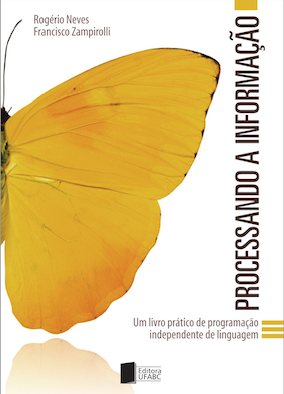
\includegraphics{"figs/Capa_Processando_Informacao.jpg"}

Este caderno (Notebook) é parte complementar \emph{online} do livro
\textbf{\href{https://editora.ufabc.edu.br/matematica-e-ciencias-da-computacao/58-processando-a-informacao}{Processando
a Informação}: um livro prático de programação independente de
linguagem}, que deve ser consultado no caso de dúvidas sobre os temas
apresentados.

\begin{quote}
Este conteúdo pode ser copiado e alterado livremente e foi inspirado
nesse livro.
\end{quote}

    \hypertarget{instruuxe7uxf5es}{%
\subsubsection{Instruções}\label{instruuxe7uxf5es}}

    \begin{itemize}
\tightlist
\item
  A lista de exercícios PODERÁ NÃO SER AVALIADA PELO PROFESSOR, mas
  entre em contato com o monitor ou o professor se tiver alguma dúvida.
\item
  É recomendado tirar uma cópia do notebook clicando na opção
  \textbf{``copiar para o drive''} no menu acima à direita (você precisa
  estar logado na sua conta no Google para fazer isto).
  Alternativamente, selecione
  \textbf{``Arquivo''}--\textgreater{}\textbf{``Salvar cópia no
  drive''}. Desta forma você poderá editá-lo e executar os campos de
  código sempre que quiser, sem perder os seu progresso ao fechar esta
  página.
\item
  Após digitar o código pedido no campo indicado, clique no botão
  \textbf{``executar''} ou \textbf{``play''} para ver a saída do código
  entrado.
\item
  É recomendado seguir a ordem sugerida dos exercícios, uma vez que
  familiaridade com os conceitos introduzidos são esperados nos
  exercícios seguintes.
\item
  O \emph{notebook Colab} tem o Python nativo para rodar as células de
  código. Se desejar outra linguagem de programação, consulte o material
  do Capítulo 1, na pasta do Google Drive
  \href{https://drive.google.com/drive/folders/1YlFwv8XYN7PYYf-HwDMlkxzbmXzJw9cM?usp=sharing}{colabs}
\end{itemize}

    \hypertarget{sugestuxf5es-para-envio-dos-exercuxedcios-com-avaliauxe7uxe3o-automuxe1tica-no-moodlevpl}{%
\subsubsection{Sugestões para envio dos exercícios com avaliação
automática no
Moodle+VPL}\label{sugestuxf5es-para-envio-dos-exercuxedcios-com-avaliauxe7uxe3o-automuxe1tica-no-moodlevpl}}

    \begin{itemize}
\tightlist
\item
  Fique atento as datas de entrega no calendário do Moodle.
\item
  Escolha uma linguagem de programação para submeter os exercícios (ou a
  definida pelo seu professor).
\item
  A atividade no Moodle considera sempre a última submissão, com a nota
  atribuída de forma automática.
\item
  Faça uma cópia do Colab e tente resolver as questões aqui, ou em
  alguma IDE de sua preferência, antes de enviar para avaliação no
  Moodle.
\item
  É possível rodar códigos independentes em IDEs e também \emph{online},
  utilizando navegadores como o chrome: https://ideone.com/,
  https://www.codechef.com/ide, https://replit.com/,
  https://www.jdoodle.com.
\item
  É possível também rodar códigos no seu celular, utilizando navegadores
  acessando esses links.
\end{itemize}

    \hypertarget{exercuxedcios}{%
\subsubsection{Exercícios}\label{exercuxedcios}}

    \begin{center}\rule{0.5\linewidth}{0.5pt}\end{center}

\begin{enumerate}
\def\labelenumi{\arabic{enumi}.}
\tightlist
\item
  No espaço abaixo, escreva um programa para exibir a mensagem ``Alô
  mundo!''. Execute-o e verifique se a saída está correta.
\end{enumerate}

    \begin{center}\rule{0.5\linewidth}{0.5pt}\end{center}

\begin{enumerate}
\def\labelenumi{\arabic{enumi}.}
\setcounter{enumi}{1}
\tightlist
\item
  \textbf{Complete} o processamento do código abaixo com a fórmula
  correta para o delta (\(\Delta = b^2-4ac\)) da equação do segundo
  grau, na forma \(ax^{2}+bx+c=0\). \textbf{Dados}: a operação `elevado'
  em Python é \texttt{**}. Considere alguns valores inteiros e reais
  para \(a\), \(b\) e \(c\). \textbf{Resposta correta:} delta = 49
\end{enumerate}

\begin{verbatim}
a = 2
b = 3
c = -5
\end{verbatim}

    \begin{center}\rule{0.5\linewidth}{0.5pt}\end{center}

\begin{enumerate}
\def\labelenumi{\arabic{enumi}.}
\setcounter{enumi}{2}
\tightlist
\item
  \textbf{Complete o código anterior} no campo abaixo com comandos para
  calcular e exibir as raízes da equação do segundo grau, usando a
  fórmula \(raiz_1=\frac{-b+\sqrt{\Delta}}{2a}\) e
  \(raiz_2=\frac{-b-\sqrt{\Delta}}{2a}\). \textbf{Dados}: raiz de um
  número = número**.5 (elevado a meio). \textbf{Respostas:} (-2.5, 1.0).
\end{enumerate}

    \begin{center}\rule{0.5\linewidth}{0.5pt}\end{center}

\begin{enumerate}
\def\labelenumi{\arabic{enumi}.}
\setcounter{enumi}{3}
\tightlist
\item
  Adicione \texttt{código} na parte indicada para trocar os valores das
  variáveis \texttt{a,\ b\ e\ c} (definidas anteriormente) de forma que
  \texttt{a} contenha o menor valor, \texttt{b} contenha o valor central
  e \texttt{c} contenha o maior valor. A última linha
  \texttt{(a,\ b,\ c)} não deve ser alterada. \textbf{Saída}:
  \texttt{(-5,\ 2,\ 3)}
\end{enumerate}

    \begin{center}\rule{0.5\linewidth}{0.5pt}\end{center}

\begin{enumerate}
\def\labelenumi{\arabic{enumi}.}
\setcounter{enumi}{4}
\tightlist
\item
  Escreva abaixo um programa completo que leia dois números (devem ser
  digitados pelo usuário) e calcule e exiba a média. Quando executado, o
  programa deve gerar a seguinte saída:
\end{enumerate}

\begin{verbatim}
Entre com o primeiro número: 10
Entre com o segundo número: 5
Média: 7.5
\end{verbatim}

    \hypertarget{processando-a-informauxe7uxe3o-cap.-1-fundamentos---pruxe1tica-2}{%
\subsection{Processando a Informação: Cap. 1: Fundamentos - Prática
2}\label{processando-a-informauxe7uxe3o-cap.-1-fundamentos---pruxe1tica-2}}

    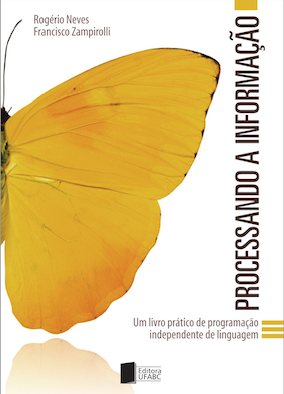
\includegraphics{"figs/Capa_Processando_Informacao.jpg"}

Este caderno (Notebook) é parte complementar \emph{online} do livro
\textbf{\href{https://editora.ufabc.edu.br/matematica-e-ciencias-da-computacao/58-processando-a-informacao}{Processando
a Informação}: um livro prático de programação independente de
linguagem}, que deve ser consultado no caso de dúvidas sobre os temas
apresentados.

\begin{quote}
Este conteúdo pode ser copiado e alterado livremente e foi inspirado
nesse livro.
\end{quote}

    \hypertarget{exercuxedcios}{%
\subsubsection{Exercícios}\label{exercuxedcios}}

{[}Fonte: https://wiki.python.org.br/EstruturaSequencial{]}

    \begin{center}\rule{0.5\linewidth}{0.5pt}\end{center}

\begin{enumerate}
\def\labelenumi{\arabic{enumi}.}
\tightlist
\item
  Faça um programa que peça o raio (\(R\)) de um círculo, calcule e
  mostre sua área (\(\pi R^2\)) e seu perímetro (\(2\pi R\)).
\end{enumerate}

    \begin{center}\rule{0.5\linewidth}{0.5pt}\end{center}

\begin{enumerate}
\def\labelenumi{\arabic{enumi}.}
\setcounter{enumi}{1}
\tightlist
\item
  Faça um programa que peça a Apótema (\(a\), ver figura), o número
  (\(n\)) de lados do polígono regular e o comprimento \(l\) de cada
  lado. Calcule e mostre a sua Área (\(A=nla/2\)). Essa fórmula funciona
  para triângulo equilátero e quadrado?
  {[}\href{https://www.todamateria.com.br/area-dos-poligonos/amp/}{fonte}{]}
\end{enumerate}

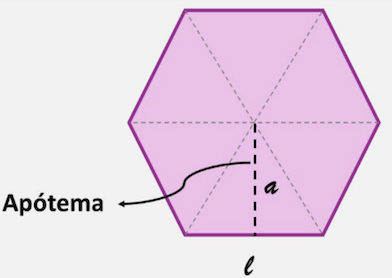
\includegraphics{"figs/poligono.png"}

    \begin{center}\rule{0.5\linewidth}{0.5pt}\end{center}

\begin{enumerate}
\def\labelenumi{\arabic{enumi}.}
\setcounter{enumi}{2}
\tightlist
\item
  Faça um programa que pergunte quanto você ganha por hora e o número de
  horas trabalhadas por dia da semana (sem sábados e domingos). Calcule
  e mostre o total do seu salário semanal.
\end{enumerate}

    \begin{center}\rule{0.5\linewidth}{0.5pt}\end{center}

\begin{enumerate}
\def\labelenumi{\arabic{enumi}.}
\setcounter{enumi}{3}
\tightlist
\item
  Faça um programa que peça a temperatura em graus Fahrenheit,
  transforme e mostre a temperatura em graus Celsius.
\end{enumerate}

    \begin{center}\rule{0.5\linewidth}{0.5pt}\end{center}

\begin{enumerate}
\def\labelenumi{\arabic{enumi}.}
\setcounter{enumi}{4}
\tightlist
\item
  Faça um programa que peça 2 números inteiros e um número real. Calcule
  e mostre:
\end{enumerate}

\begin{itemize}
\tightlist
\item
  o produto do dobro do primeiro com metade do segundo;
\item
  a soma do triplo do primeiro com o terceiro;
\item
  o terceiro elevado ao cubo.
\end{itemize}

    \begin{center}\rule{0.5\linewidth}{0.5pt}\end{center}

\begin{enumerate}
\def\labelenumi{\arabic{enumi}.}
\setcounter{enumi}{5}
\tightlist
\item
  Tendo como dados de entrada a altura (\(h\)) de uma pessoa, construa
  um programa que calcule seu peso ideal, usando a seguinte fórmula:
  \[72.7h - 58\]
\end{enumerate}

    \begin{center}\rule{0.5\linewidth}{0.5pt}\end{center}

\begin{enumerate}
\def\labelenumi{\arabic{enumi}.}
\setcounter{enumi}{6}
\tightlist
\item
  Tendo como dado de entrada a altura (\(h\)) de uma pessoa, construa um
  programa que calcule seu peso ideal, utilizando as seguintes fórmulas:
\end{enumerate}

\begin{itemize}
\tightlist
\item
  homens: \(72.7h - 58\)
\item
  mulheres: \(62.1h - 44.7\)
\end{itemize}

    \begin{center}\rule{0.5\linewidth}{0.5pt}\end{center}

\begin{enumerate}
\def\labelenumi{\arabic{enumi}.}
\setcounter{enumi}{7}
\tightlist
\item
  João Papo-de-Pescador, homem de bem, comprou um microcomputador para
  controlar o rendimento diário de seu trabalho. Considere que ele
  sempre traz um peso de peixes maior que o estabelecido pelo
  regulamento de pesca do estado de São Paulo (50 quilos), neste caso,
  com uma multa de R\$ 4,00 por quilo excedente. João precisa que você
  faça um programa que leia a variável peso (peso de peixes) e calcule o
  excesso. Gravar na variável excesso a quantidade de quilos além do
  limite e na variável multa o valor da multa que João deverá pagar.
  Imprima os dados do programa com as mensagens adequadas.
\end{enumerate}

    \begin{center}\rule{0.5\linewidth}{0.5pt}\end{center}

\begin{enumerate}
\def\labelenumi{\arabic{enumi}.}
\setcounter{enumi}{8}
\tightlist
\item
  Faça um programa que pergunte quanto você ganha por hora e o número de
  horas trabalhadas no mês. Calcule e mostre o total do seu salário no
  referido mês, sabendo-se que são descontados 11\% para o Imposto de
  Renda, 8\% para o INSS e 5\% para o sindicato, faça um programa que
  nos dê:
\end{enumerate}

\begin{itemize}
\tightlist
\item
  salário bruto.
\item
  quanto pagou ao INSS.
\item
  quanto pagou ao sindicato.
\item
  o salário líquido.
\item
  calcule os descontos e o salário líquido, conforme a tabela abaixo:
\end{itemize}

\begin{verbatim}
  + Salário Bruto : R$
  - IR (11%) : R$
  - INSS (8%) : R$
  - Sindicato  (5%) : R$
  = Salário Liquido : R$
\end{verbatim}

Obs.: Salário Bruto - Descontos = Salário Líquido

    \begin{center}\rule{0.5\linewidth}{0.5pt}\end{center}

\begin{enumerate}
\def\labelenumi{\arabic{enumi}.}
\setcounter{enumi}{9}
\tightlist
\item
  Faça um programa para uma loja de tintas. O programa deverá pedir o
  tamanho em metros quadrados da área a ser pintada. Considere que a
  cobertura da tinta é de 1 litro para cada 3 metros quadrados e que a
  tinta é vendida em latas de 18 litros, que custam R\$ 80,00. Informe
  ao usuário a quantidade de latas de tinta a serem compradas e o preço
  total.
\end{enumerate}

    \hypertarget{processando-a-informauxe7uxe3o-cap.-1-fundamentos---pruxe1tica-4-tutorial-vscode}{%
\subsection{Processando a Informação: Cap. 1: Fundamentos - Prática 4:
Tutorial
VSCode}\label{processando-a-informauxe7uxe3o-cap.-1-fundamentos---pruxe1tica-4-tutorial-vscode}}

    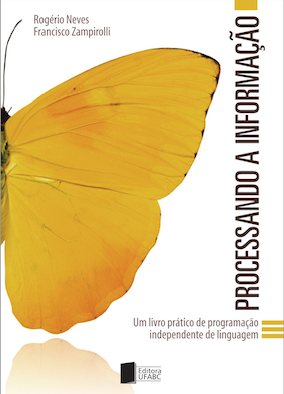
\includegraphics{"figs/Capa_Processando_Informacao.jpg"}

Este caderno (Notebook) é parte complementar \emph{online} do livro
\textbf{\href{https://editora.ufabc.edu.br/matematica-e-ciencias-da-computacao/58-processando-a-informacao}{Processando
a Informação}: um livro prático de programação independente de
linguagem}, que deve ser consultado no caso de dúvidas sobre os temas
apresentados.

\begin{quote}
Este conteúdo pode ser copiado e alterado livremente e foi inspirado
nesse livro.
\end{quote}

    \hypertarget{tuturial-em-construuxe7uxe3o-vscode}{%
\subsubsection{Tuturial (em construção)
VSCode}\label{tuturial-em-construuxe7uxe3o-vscode}}

    \begin{itemize}
\item
  \textbf{\href{https://vscode.dev}{VSCODE}} - versão \emph{online} de
  código aberto do \emph{Visual studio}.
\item
  Para download e uso local: https://code.visualstudio.com/download.
\item
  Ver:

  \begin{itemize}
  \tightlist
  \item
    https://docs.microsoft.com/pt-br/learn/modules/introduction-to-github-visual-studio-code/
  \item
    https://www.digitalocean.com/community/tutorials/how-to-use-git-integration-in-visual-studio-code-pt
  \item
    https://balta.io/blog/git-github-primeiros-passos
  \end{itemize}
\item
  Clonar: https://github.com/fzampirolli/codigosPE
\item
  Alterar \texttt{settings.json} em \texttt{code-runner.executorMap}:

  \begin{itemize}
  \tightlist
  \item
    \texttt{"c":\ "cd\ \$dir\ \&\&\ gcc\ -Wall\ -std=c99\ \$fileName\ -o\ ...}

    \begin{itemize}
    \tightlist
    \item
      \texttt{-Wall} para mostrar \texttt{warning} (programas ruins)
    \item
      \texttt{-std=c99} - padrão ANSI ou
      \href{https://en.m.wikipedia.org/wiki/C99}{C99}, os programas
      seguindo esse padrão são mais portáveis, ou seja, possuem menos
      problemas de compatibilidade entre diferentes arquiteturas.
    \end{itemize}
  \end{itemize}
\end{itemize}

    \hypertarget{processando-a-informauxe7uxe3o-cap.-2-organizauxe7uxe3o-de-cuxf3digo}{%
\section{Processando a Informação: Cap. 2: Organização de
código}\label{processando-a-informauxe7uxe3o-cap.-2-organizauxe7uxe3o-de-cuxf3digo}}

    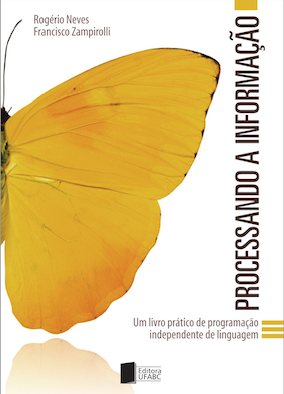
\includegraphics{"figs/Capa_Processando_Informacao.jpg"}

Este caderno (Notebook) é parte complementar \emph{online} do livro
\textbf{\href{https://editora.ufabc.edu.br/matematica-e-ciencias-da-computacao/58-processando-a-informacao}{Processando
a Informação}: um livro prático de programação independente de
linguagem}, que deve ser consultado no caso de dúvidas sobre os temas
apresentados.

\begin{quote}
Este conteúdo pode ser copiado e alterado livremente e foi inspirado
nesse livro.
\end{quote}

    \hypertarget{sumuxe1rio}{%
\subsection{Sumário}\label{sumuxe1rio}}

\begin{itemize}
\tightlist
\item
  Revisão do capítulo anterior
\item
  Programas sequenciais
\item
  Comentários
\item
  Desvios de fluxo
\item
  Programas e Subprogramas
\item
  Funções, métodos e modularização
\item
  Reaproveitamento e manutenção de código
\item
  Revisão deste capítulo
\item
  Exercícios
\end{itemize}

    \hypertarget{revisuxe3o-do-capuxedtulo-anterior-fundamentos}{%
\subsection{Revisão do capítulo anterior
(Fundamentos)}\label{revisuxe3o-do-capuxedtulo-anterior-fundamentos}}

    \begin{itemize}
\item
  No capítulo anterior foram apresentados os fundamentos para se iniciar
  a programar utilizando alguma linguagem de programação, além de alguns
  exemplos de códigos e principalmente de como executar estes códigos em
  ambientes de programação.
\item
  Neste capítulo iremos iniciar a organizar esses códigos, utilizando o
  conceito de sistema de informação em partes:

  \begin{itemize}
  \tightlist
  \item
    \textbf{ENTRADA DE DADOS \(\Rightarrow\) PROCESSAMENTO DA INFORMAÇÃO
    \(\Rightarrow\) SAÍDA}
  \end{itemize}
\end{itemize}

    \hypertarget{programas-sequenciais}{%
\subsection{Programas sequenciais}\label{programas-sequenciais}}

    \begin{itemize}
\item
  Como vimos no capítulo anterior, um programa consiste de uma
  \textbf{sequência lógica de comandos e operações} que, executadas em
  ordem, realizam uma determinada tarefa.
\item
  Em geral, um programa processa dados de entrada de forma a obter o
  resultado desejado ou saída.
\item
  A \textbf{entrada} e a \textbf{saída} de dados são, comumente,
  realizadas utilizando os dispositivos de entrada e saída, como teclado
  e monitor.
\item
  Os dados requeridos para o \textbf{processamento} podem estar também
  contidos no código do programa (no exemplo a seguir, poderia ser
  \texttt{conta\ =\ 100}).
\item
  No exemplo a seguir em \textbf{pseudocódigo} a entrada é lida do
  teclado (comando \texttt{leia()}) e a saída é impressa no monitor
  (comando \texttt{escreva}).
\end{itemize}

    \begin{verbatim}
#1 ENTRADA de dados:
#1.1 Definição das variáveis do programa:
Real: conta, gorjeta;

#1.2 Entrada de dados
conta = leia("Entre o valor da conta: ");

#2 PROCESSAMENTO:
gorjeta = conta * 0.2;

#3 SAÍDA de dados (na tela):
escreva("Valor da gorjeta = " + gorjeta);
\end{verbatim}

    Assim, o procedimento para especificar um programa é definir: 1. Os
dados de \textbf{entrada} necessários (insumos) 2. O
\textbf{processamento} ou transformação dos dados de entrada em saída 3.
A \textbf{saída} desejada do programa

    \hypertarget{comentuxe1rios}{%
\subsection{Comentários}\label{comentuxe1rios}}

    \begin{itemize}
\tightlist
\item
  Comentários são partes do código usados pelo desenvolvedor para deixar
  notas, explicações, exemplos, etc.
\item
  Quando definido um comentário, é dada uma instrução direta ao
  \textbf{compilador/interpretador para ignorar a parte comentada}.
\item
  Isto quer dizer que os comentários não serão considerados quando o
  código for executado.
\item
  Logo, os comentários não são parte da execução.
\item
  Cada linguagem tem sua própria maneira de introduzir comentários no
  código.
\end{itemize}

    \begin{longtable}[]{@{}lll@{}}
\toprule
Tabela. Identificadores de comentário. & &\tabularnewline
\midrule
\endhead
Linguagem & Uma linha & Várias linhas\tabularnewline
Java/JS/C/C++ & //\ldots{} & /*\ldots*/\tabularnewline
Python & \#\ldots{} & ""``\ldots{}''"" ou
'\,'`\ldots{}''\,'\tabularnewline
Matlab & \%\ldots{} & \%\{\ldots\}\%\tabularnewline
Pascal & \{\ldots\} & \{\emph{\ldots{}}\}\tabularnewline
SQL & --\ldots{} & /\emph{\ldots{}}/\tabularnewline
R & \#.. &\tabularnewline
\bottomrule
\end{longtable}

    \hypertarget{desvio-de-fluxo}{%
\subsection{Desvio de Fluxo}\label{desvio-de-fluxo}}

    \begin{itemize}
\item
  Um programa consiste em uma sequência de comandos executados em ordem,
  em uma linha contínua de execução.
\item
  No entanto, esta linha (em inglês: \emph{thread}) pode conter desvios
  ou descontinuidades, processando códigos de bibliotecas ou
  subprogramas.
\end{itemize}

    \hypertarget{programas-e-subprogramas}{%
\subsection{Programas e Subprogramas}\label{programas-e-subprogramas}}

    \begin{itemize}
\item
  Em grande parte das linguagens de programação, \textbf{o código dos
  programas pode ser dividido em um ou mais arquivos ou partes}.
\item
  Cada parte contem uma sequência de comandos com um objetivo,
  realizando uma tarefa dentro do programa.
\item
  Dentro de um mesmo programa podem existir \textbf{subprogramas} (ou
  partes) com funções específicas ou subconjuntos de comandos que só
  serão executados em condições especiais.
\item
  Todas as linguagens vêm acompanhadas de \textbf{bibliotecas}, estas
  contendo funções ou programas de uso comum.
\item
  São exemplos as funções para cálculos matemáticos, para operações de
  entrada e saída, para comunicação e conversão de dados.
\end{itemize}

    \hypertarget{bibliotecas}{%
\subsection{Bibliotecas}\label{bibliotecas}}

    Cada linguagem de programação possui um conjunto de bibliotecas
disponíveis para uso. As bibliotecas podem guardar variáveis ou funções.

    \hypertarget{funuxe7uxf5es-ou-muxe9todos-de-usuuxe1rio}{%
\subsection{Funções ou Métodos de
Usuário}\label{funuxe7uxf5es-ou-muxe9todos-de-usuuxe1rio}}

    \begin{itemize}
\item
  O uso de funções facilita a \textbf{reutilização de código}, dado que
  uma função é um programa autocontido, com \textbf{entrada},
  \textbf{processamento} e \textbf{saída}.
\item
  Uma função pode ser copiada de um programa para outro ou incorporado
  em uma biblioteca escrita pelo usuário, utilizando o comando em Python
  \texttt{import\ myBiblioteca}. Ou também, para C/C++/Java,
  \texttt{\#include\ "myBiblioteca.h"}.
\item
  Uma função é definida por um nome, retorno (opcional), argumento(s)
  (opcional) e um conjunto de instruções.
\item
  A seguir temos um exemplo de função de usuário escrita em
  pseudocódigo:
\end{itemize}

    \begin{verbatim}
# MINHA(S) FUNÇÃO(ÕES)
função delta(recebe: real a, real b, real c) retorna real d {
     d = b2 – 4ac
     retorne d
}

principal {
  # ENTRADAS
  a = 5
  b = -2
  c = 4

  # PROCESSAMENTO
  real valor = delta(a, b, c) # AQUI ESTÁ A CHAMADA DA FUNÇÃO
  
  # SAÍDA
  escreva(“O delta de ax2 +bx + c é ” + valor)
}
\end{verbatim}

    \begin{verbatim}
TERMINOLOGIA: Os métodos podem ser chamados também de 
módulos, funções, subprogramas ou procedimentos. 

Existe uma convenção: quando um método tem argumento(s) 
(parâmetros) e um retorno é chamado de função, caso contrário, 
é chamado procedimento. 

Porém, poucas linguagens fazem distinção na sintaxe entre 
função e procedimento, como a Pascal, tornando confusa 
esta convenção. 
\end{verbatim}

    \hypertarget{exemplo-01---uso-de-funuxe7uxf5es}{%
\paragraph{Exemplo 01 - Uso de
Funções}\label{exemplo-01---uso-de-funuxe7uxf5es}}

    Casos para Teste Moodle+VPL

Para o professor criar uma atividade VPL no Moodle para este Exemplo 01,
basta incluir em \texttt{Casos\ para\ teste}, o seguinte texto (pode
incluir mais casos):

\begin{verbatim}
case=caso1
output= 
O delta de ax^2 + bx + c é -76.0
\end{verbatim}

    \begin{itemize}
\item
  Quando uma função não tem \texttt{return} ela deve retornar o tipo
  \texttt{void} (nada), por exemplo,
  \texttt{void\ escrevaDelta(float\ d)\{...\}}.
\item
  Os argumentos de uma função podem ser passados por \textbf{valor} ou
  por \textbf{referência}.
\item
  Por \textbf{valor}: qualquer alteração do argumento dentro da função
  não será passada para quem chamou a função.
\item
  Por \textbf{referência}: oposto ao anterior, qualquer alteração dentro
  da função será repassada para quem chamou e isso ocorre passando o
  endereço de memória da variável (com \texttt{\&}) ao ser chamado. Por
  exemplo: * \texttt{incrementaUm(\&x)}
\item
  Esse endereço de memória é definido como o tipo de dados
  \textbf{ponteiro} e será estudado em detalhes na parte de alocação
  estática vs dinâmicas.
\item
  Para acessar o conteúdo de uma variável ponteiro, usar o prefixo
  \texttt{*}. Por exemplo:

  \begin{itemize}
  \item
\begin{verbatim}
  void incrementaUm(int *x) {
      *x=*x+1;
  }
\end{verbatim}
  \end{itemize}
\item
  Observe que o \textbf{ESCOPO} da função é definido por \texttt{\{}
  \ldots{} \texttt{\}}.
\end{itemize}

    \begin{tcolorbox}[breakable, size=fbox, boxrule=1pt, pad at break*=1mm,colback=cellbackground, colframe=cellborder]
\prompt{In}{incolor}{9}{\boxspacing}
\begin{Verbatim}[commandchars=\\\{\}]
\PY{o}{\PYZpc{}\PYZpc{}writefile} cap2ex01.c
\PY{c+c1}{\PYZsh{}include \PYZlt{}stdio.h\PYZgt{}}
\PY{o}{/}\PY{o}{/} \PY{n}{MÉTODO}

\PY{n+nb}{float} \PY{n}{delta}\PY{p}{(}\PY{n+nb}{float} \PY{n}{a}\PY{p}{,} \PY{n+nb}{float} \PY{n}{b}\PY{p}{,} \PY{n+nb}{float} \PY{n}{c}\PY{p}{)} \PY{p}{\PYZob{}}
  \PY{n+nb}{float} \PY{n}{d} \PY{o}{=} \PY{n}{b} \PY{o}{*} \PY{n}{b} \PY{o}{\PYZhy{}} \PY{l+m+mi}{4} \PY{o}{*} \PY{n}{a} \PY{o}{*} \PY{n}{c}\PY{p}{;}
  \PY{k}{return} \PY{n}{d}\PY{p}{;}
\PY{p}{\PYZcb{}}
\PY{o}{/}\PY{o}{/} \PY{n}{PROGRAMA} \PY{n}{PRINCIPAL}
\PY{n+nb}{int} \PY{n}{main}\PY{p}{(}\PY{n}{void}\PY{p}{)} \PY{p}{\PYZob{}}
  \PY{n+nb}{float} \PY{n}{a} \PY{o}{=} \PY{l+m+mf}{5.0}\PY{p}{,} \PY{n}{b} \PY{o}{=} \PY{o}{\PYZhy{}}\PY{l+m+mf}{2.0}\PY{p}{,} \PY{n}{c} \PY{o}{=} \PY{l+m+mf}{4.0}\PY{p}{;}
  \PY{n}{printf}\PY{p}{(}\PY{l+s+s2}{\PYZdq{}}\PY{l+s+s2}{O delta de ax\PYZca{}2 + bx + c e }\PY{l+s+si}{\PYZpc{}.1f}\PY{l+s+se}{\PYZbs{}n}\PY{l+s+s2}{\PYZdq{}}\PY{p}{,} \PY{n}{delta}\PY{p}{(}\PY{n}{a}\PY{p}{,} \PY{n}{b}\PY{p}{,} \PY{n}{c}\PY{p}{)}\PY{p}{)}\PY{p}{;}
  \PY{k}{return} \PY{l+m+mi}{0}\PY{p}{;}
\PY{p}{\PYZcb{}}
\end{Verbatim}
\end{tcolorbox}

    \begin{tcolorbox}[breakable, size=fbox, boxrule=1pt, pad at break*=1mm,colback=cellbackground, colframe=cellborder]
\prompt{In}{incolor}{10}{\boxspacing}
\begin{Verbatim}[commandchars=\\\{\}]
\PY{o}{\PYZpc{}\PYZpc{}}\PY{k}{shell}
gcc \PYZhy{}Wall \PYZhy{}std=c99 cap2ex01.c \PYZhy{}o output2
./output2
\end{Verbatim}
\end{tcolorbox}

    \hypertarget{tabulauxe7uxe3o}{%
\subsubsection{Tabulação}\label{tabulauxe7uxe3o}}

    \begin{itemize}
\item
  Um conceito muito importante em programação é a ``endentação''
  (\emph{indentation}) ou tabulação do código.
\item
  Note que sempre que um bloco ou subconjunto de comandos é iniciado com
  \texttt{\{} a tabulação é incrementada, e quando um subconjunto de
  comandos se encerra com \texttt{\}} a tabulação é recuada.
\item
  Isto permite visualizar claramente quando um grupo de comandos define
  um subprograma.
\item
  Alguns editores de programa e a maioria das IDEs já fazem a tabulação
  de forma automática. Pesquise como fazer isso em uma IDE que esteja
  utilizando.
\item
  Códigos sem tabulações corretas são muito difíceis de ler por outra
  pessoa (\textbf{os professores geralmente descontam pontos em códigos
  desorganizados!}).
\end{itemize}

    \hypertarget{escopo}{%
\subsection{Escopo}\label{escopo}}

    \begin{itemize}
\item
  Os subprogramas são programas independentes dentro do programa.
\item
  Logo possuem variáveis próprias para armazenar seus dados.
\item
  Estas \textbf{variáveis locais} só existem no âmbito do subprograma e
  só durante cada execução (chamada) do mesmo, desaparecendo (ou sendo
  apagadas) ao término do subprograma ou ao retornar em qualquer ponto
  com o comando \texttt{return}.
\item
  \textbf{Variáveis globais}, por outro lado, podem ser criadas em um
  escopo hierarquicamente superior a todos os métodos/funções, desta
  forma permeando todos os subprogramas.
\item
  Logo, as \textbf{variáveis globais} têm escopo em todos os métodos.
\end{itemize}

    \hypertarget{reaproveitamento-e-manutenuxe7uxe3o-de-cuxf3digo}{%
\subsection{Reaproveitamento e Manutenção de
Código}\label{reaproveitamento-e-manutenuxe7uxe3o-de-cuxf3digo}}

    \begin{itemize}
\item
  Outra vantagem do uso de funções/métodos, além da capacidade de se
  reaproveitar o código já escrito em novos programas copiando os
  subprogramas desejados, é

  \begin{itemize}
  \tightlist
  \item
    a possibilidade de se atualizar os métodos sem a necessidade de
    alterar o código do programa principal.
  \end{itemize}
\item
  Para tanto, basta que a comunicação do método (entradas e saídas)
  permaneça inalterada.
\item
  Como exemplo, utilizamos um programa com métodos para entrada e saída
  de dados com os métodos/funções \texttt{leia()} e \texttt{escreva()},
  baseado nos exemplos anteriores.
\item
  Para programas muito simples, como poucas linhas de código, pode ter a
  impressão de deixar o código mais complicado, mas a principal vantagem
  é o reaproveitamento de código em outros programas similares.
\item
  Esse recurso de métodos de entrada e saída serão muito úteis nos
  tópicos de Vetores e Matrízes, abordados nos Capítulos 5 e 6,
  respectivamente,

  \begin{itemize}
  \tightlist
  \item
    quando funções para ler e escrever um vetor/matriz poderão ser
    reaproveitados em várias questões.
  \end{itemize}
\end{itemize}

    \hypertarget{exemplo-02---uso-de-funuxe7uxf5es-com-entrada-e-sauxedda-de-dados}{%
\paragraph{Exemplo 02 - Uso de Funções com Entrada e Saída de
Dados}\label{exemplo-02---uso-de-funuxe7uxf5es-com-entrada-e-sauxedda-de-dados}}

    Casos para Teste no Moodle+VPL

Para o professor criar uma atividade VPL no Moodle para este Exemplo 02,
basta incluir em \texttt{Casos\ para\ teste}, o seguinte texto (pode
incluir mais casos):

\begin{verbatim}
case=caso1
input=3
4
5
output= 
-44.0
case=caso2
input=3
4
2
output= 
-8.0
case=caso3
input=3
5
2
output= 
1.0
\end{verbatim}

    \begin{tcolorbox}[breakable, size=fbox, boxrule=1pt, pad at break*=1mm,colback=cellbackground, colframe=cellborder]
\prompt{In}{incolor}{11}{\boxspacing}
\begin{Verbatim}[commandchars=\\\{\}]
\PY{o}{\PYZpc{}\PYZpc{}writefile} cap2ex02.c
\PY{c+c1}{\PYZsh{}include \PYZlt{}stdio.h\PYZgt{}}

\PY{n+nb}{float} \PY{n}{delta}\PY{p}{(}\PY{n+nb}{float} \PY{n}{a}\PY{p}{,} \PY{n+nb}{float} \PY{n}{b}\PY{p}{,} \PY{n+nb}{float} \PY{n}{c}\PY{p}{)} \PY{p}{\PYZob{}}
  \PY{n+nb}{float} \PY{n}{d} \PY{o}{=} \PY{n}{b}\PY{o}{*}\PY{n}{b}\PY{o}{\PYZhy{}}\PY{l+m+mi}{4}\PY{o}{*}\PY{n}{a}\PY{o}{*}\PY{n}{c}\PY{p}{;}
  \PY{k}{return} \PY{n}{d}\PY{p}{;}
\PY{p}{\PYZcb{}}

\PY{n+nb}{float} \PY{n}{leia}\PY{p}{(}\PY{p}{)} \PY{p}{\PYZob{}}
  \PY{n+nb}{float} \PY{n}{valor}\PY{p}{;}
  \PY{n}{printf}\PY{p}{(}\PY{l+s+s2}{\PYZdq{}}\PY{l+s+s2}{Entre com um valor: }\PY{l+s+s2}{\PYZdq{}}\PY{p}{)}\PY{p}{;}
  \PY{n}{scanf}\PY{p}{(}\PY{l+s+s2}{\PYZdq{}}\PY{l+s+si}{\PYZpc{}f}\PY{l+s+s2}{\PYZdq{}}\PY{p}{,} \PY{o}{\PYZam{}}\PY{n}{valor}\PY{p}{)}\PY{p}{;}
  \PY{k}{return} \PY{n}{valor}\PY{p}{;}
\PY{p}{\PYZcb{}}

\PY{n+nb}{int} \PY{n}{main}\PY{p}{(}\PY{n}{void}\PY{p}{)} \PY{p}{\PYZob{}}

  \PY{o}{/}\PY{o}{/} \PY{n}{ENTRADAS}
  \PY{n+nb}{float} \PY{n}{a}\PY{p}{,} \PY{n}{b}\PY{p}{,} \PY{n}{c}\PY{p}{,} \PY{n}{d}\PY{p}{;}
  \PY{n}{a} \PY{o}{=} \PY{n}{leia}\PY{p}{(}\PY{p}{)}\PY{p}{;}
  \PY{n}{b} \PY{o}{=} \PY{n}{leia}\PY{p}{(}\PY{p}{)}\PY{p}{;}
  \PY{n}{c} \PY{o}{=} \PY{n}{leia}\PY{p}{(}\PY{p}{)}\PY{p}{;}
  
  \PY{o}{/}\PY{o}{/} \PY{n}{PROCESSAMENTO}
  \PY{n}{d} \PY{o}{=} \PY{n}{delta}\PY{p}{(}\PY{n}{a}\PY{p}{,} \PY{n}{b}\PY{p}{,} \PY{n}{c}\PY{p}{)}\PY{p}{;}

  \PY{o}{/}\PY{o}{/}\PY{n}{SAÍDA}
  \PY{n}{printf}\PY{p}{(}\PY{l+s+s2}{\PYZdq{}}\PY{l+s+s2}{Delta = }\PY{l+s+si}{\PYZpc{}.1f}\PY{l+s+s2}{\PYZdq{}}\PY{p}{,} \PY{n}{d}\PY{p}{)}\PY{p}{;}
  \PY{k}{return} \PY{l+m+mi}{0}\PY{p}{;}
\PY{p}{\PYZcb{}}
\end{Verbatim}
\end{tcolorbox}

    \begin{tcolorbox}[breakable, size=fbox, boxrule=1pt, pad at break*=1mm,colback=cellbackground, colframe=cellborder]
\prompt{In}{incolor}{12}{\boxspacing}
\begin{Verbatim}[commandchars=\\\{\}]
\PY{o}{\PYZpc{}\PYZpc{}}\PY{k}{shell}
gcc \PYZhy{}Wall \PYZhy{}std=c99 cap2ex02.c \PYZhy{}o output2
./output2
\end{Verbatim}
\end{tcolorbox}

    \hypertarget{exercuxedcios}{%
\subsection{Exercícios}\label{exercuxedcios}}

    Ver notebook Colab no arquivo \texttt{cap2.part2.lab.*.ipynb}
(\texttt{*} é a extensão da linguagem), utilizando alguma linguagem de
programação de sua preferência, organizadas em subpastas contidas de
\texttt{"gen"}, na pasta do Google Drive
\href{https://drive.google.com/drive/folders/1YlFwv8XYN7PYYf-HwDMlkxzbmXzJw9cM?usp=sharing}{colabs}.

    \hypertarget{revisuxe3o-deste-capuxedtulo-de-organizauxe7uxe3o-de-cuxf3digo}{%
\subsection{Revisão deste capítulo de Organização de
Código}\label{revisuxe3o-deste-capuxedtulo-de-organizauxe7uxe3o-de-cuxf3digo}}

\begin{itemize}
\tightlist
\item
  Programas sequenciais

  \begin{itemize}
  \tightlist
  \item
    organize o seu código em três parte: \textgreater{} Entrada
    \(\Rightarrow\) Processamento \(\Rightarrow\) Saída
  \end{itemize}
\item
  Comentários

  \begin{itemize}
  \tightlist
  \item
    São úteis para outros podem ententer o seu código
  \end{itemize}
\item
  Desvios de fluxo
\item
  Programas e subprogramas
\item
  Funções, métodos e modularização
\item
  Reaproveitamento e manutenção de código

  \begin{itemize}
  \tightlist
  \item
    Esses 4 últimos tópicos são muito importantes para organizar o seu
    código em partes
  \item
    Fique atento ao \textbf{escopo} de uma variável \textbf{local} ou
    \textbf{global}
  \end{itemize}
\item
  Exercícios
\end{itemize}

    \hypertarget{processando-a-informauxe7uxe3o-cap.-2-organizauxe7uxe3o-de-cuxf3digo---pruxe1tica-1}{%
\subsection{Processando a Informação: Cap. 2: Organização de Código -
Prática
1}\label{processando-a-informauxe7uxe3o-cap.-2-organizauxe7uxe3o-de-cuxf3digo---pruxe1tica-1}}

    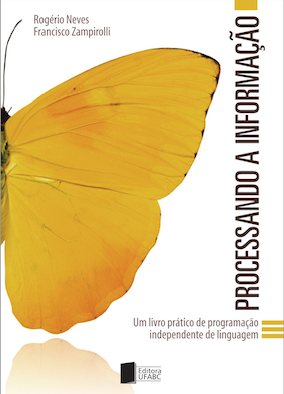
\includegraphics{"figs/Capa_Processando_Informacao.jpg"}

Este caderno (Notebook) é parte complementar \emph{online} do livro
\textbf{\href{https://editora.ufabc.edu.br/matematica-e-ciencias-da-computacao/58-processando-a-informacao}{Processando
a Informação}: um livro prático de programação independente de
linguagem}, que deve ser consultado no caso de dúvidas sobre os temas
apresentados.

\begin{quote}
Este conteúdo pode ser copiado e alterado livremente e foi inspirado
nesse livro.
\end{quote}

    \hypertarget{exercuxedcios}{%
\subsubsection{Exercícios}\label{exercuxedcios}}

    Organizar cada questão em partes:

\begin{itemize}
\tightlist
\item
  \textbf{ENTRADA DE DADOS \(\Rightarrow\) PROCESSAMENTO DA INFORMAÇÃO
  \(\Rightarrow\) SAÍDA}
\end{itemize}

Seguindo o pseudocódigo a seguir:

    \begin{verbatim}
# MINHA(S) FUNÇÃO(ÕES)
função delta(recebe: real a, real b, real c) retorna real d {
     d = b2 – 4ac
     retorne d
}

principal {
  # ENTRADAS
  a = 5
  b = -2
  c = 4

  # PROCESSAMENTO
  real valor = delta(a, b, c) # AQUI ESTÁ A CHAMADA DA FUNÇÃO
  
  # SAÍDA
  escreva(“O delta de ax2 +bx + c é ” + valor)
}
\end{verbatim}

    \begin{center}\rule{0.5\linewidth}{0.5pt}\end{center}

\begin{enumerate}
\def\labelenumi{\arabic{enumi}.}
\tightlist
\item
  Crie um método que receba um valor inteiro qualquer e retorne 0 se
  este valor for par ou 1 se for ímpar (Dica: utilizar o operador resto
  \%). Teste em um programa principal várias chamadas deste método.
\end{enumerate}

    \begin{center}\rule{0.5\linewidth}{0.5pt}\end{center}

\begin{enumerate}
\def\labelenumi{\arabic{enumi}.}
\setcounter{enumi}{1}
\tightlist
\item
  Descreva o procedimento ou função para receber um ponto em coordenadas
  cartesianas (X, Y) e retornar a distância euclidiana até a origem (0,
  0). Teste em um programa principal várias chamadas deste método.
\end{enumerate}

    \begin{center}\rule{0.5\linewidth}{0.5pt}\end{center}

\begin{enumerate}
\def\labelenumi{\arabic{enumi}.}
\setcounter{enumi}{2}
\tightlist
\item
  Crie um método para calcular o ângulo formado entre um par de pontos
  X, Y, e o eixo x no plano cartesiano. Teste em um programa principal
  várias chamadas deste método.
\end{enumerate}

    \begin{center}\rule{0.5\linewidth}{0.5pt}\end{center}

\begin{enumerate}
\def\labelenumi{\arabic{enumi}.}
\setcounter{enumi}{3}
\tightlist
\item
  Crie um método para calcular o ângulo formado entre um par de pontos
  X1, Y1 e X2, Y2 e o eixo x no plano cartesiano. Teste em um programa
  principal várias chamadas deste método.
\end{enumerate}

    \begin{center}\rule{0.5\linewidth}{0.5pt}\end{center}

\begin{enumerate}
\def\labelenumi{\arabic{enumi}.}
\setcounter{enumi}{4}
\tightlist
\item
  Crie um programa com variáveis globais de um retângulo para base,
  altura e área. Crie no mesmo programa funções para calcular cada um
  dos 3 valores a partir dos outros 2: \texttt{calcula\_base()},
  \texttt{calcula\_altura()} e \texttt{calcula\_area()}. Teste em um
  programa principal várias chamadas deste método.
\end{enumerate}

    \hypertarget{processando-a-informauxe7uxe3o-cap.-2-organizauxe7uxe3o-de-cuxf3digo---pruxe1tica-2}{%
\subsection{Processando a Informação: Cap. 2: Organização de Código -
Prática
2}\label{processando-a-informauxe7uxe3o-cap.-2-organizauxe7uxe3o-de-cuxf3digo---pruxe1tica-2}}

    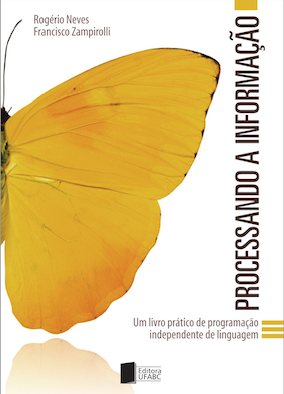
\includegraphics{"figs/Capa_Processando_Informacao.jpg"}

Este caderno (Notebook) é parte complementar \emph{online} do livro
\textbf{\href{https://editora.ufabc.edu.br/matematica-e-ciencias-da-computacao/58-processando-a-informacao}{Processando
a Informação}: um livro prático de programação independente de
linguagem}, que deve ser consultado no caso de dúvidas sobre os temas
apresentados.

\begin{quote}
Este conteúdo pode ser copiado e alterado livremente e foi inspirado
nesse livro.
\end{quote}

    \hypertarget{exercuxedcios}{%
\subsubsection{Exercícios}\label{exercuxedcios}}

    {[}Fonte: https://wiki.python.org.br/ExerciciosFuncoes{]}

Organizar cada questão em partes:

\begin{itemize}
\tightlist
\item
  \textbf{ENTRADA DE DADOS \(\Rightarrow\) PROCESSAMENTO DA INFORMAÇÃO
  \(\Rightarrow\) SAÍDA}
\end{itemize}

Seguindo o pseudocódigo a seguir:

    \begin{verbatim}
# MINHA(S) FUNÇÃO(ÕES)
função delta(recebe: real a, real b, real c) retorna real d {
     d = b2 – 4ac
     retorne d
}

principal {
  # ENTRADAS
  a = 5
  b = -2
  c = 4

  # PROCESSAMENTO
  real valor = delta(a, b, c) # AQUI ESTÁ A CHAMADA DA FUNÇÃO
  
  # SAÍDA
  escreva(“O delta de ax2 +bx + c é ” + valor)
}
\end{verbatim}

    \begin{center}\rule{0.5\linewidth}{0.5pt}\end{center}

\begin{enumerate}
\def\labelenumi{\arabic{enumi}.}
\tightlist
\item
  Fazer uma função que recebe três argumentos e retorne o produto desses
  três argumentos. Teste em um programa principal várias chamadas deste
  método.
\end{enumerate}

    \begin{center}\rule{0.5\linewidth}{0.5pt}\end{center}

\begin{enumerate}
\def\labelenumi{\arabic{enumi}.}
\setcounter{enumi}{1}
\tightlist
\item
  Faça um programa com uma função chamada \texttt{somaImposto}. A função
  possui dois parâmetros formais: taxaImposto, que é a quantia de
  imposto sobre vendas expressa em porcentagem e custo, que é o custo de
  um item antes do imposto. A função ``altera'' o valor de custo para
  incluir o imposto sobre vendas.
\end{enumerate}

    \begin{center}\rule{0.5\linewidth}{0.5pt}\end{center}

\begin{enumerate}
\def\labelenumi{\arabic{enumi}.}
\setcounter{enumi}{2}
\tightlist
\item
  Faça um programa que use a função valorPagamento para determinar o
  valor a ser pago por uma prestação de uma conta. O programa deverá
  solicitar ao usuário o valor da prestação e o número de dias em atraso
  e passar estes valores para a função valorPagamento, que calculará o
  valor a ser pago e devolverá este valor ao programa que a chamou. O
  programa deverá então exibir o valor a ser pago na tela. O cálculo do
  valor a ser pago é feito da seguinte forma. Considere que sempre tem
  atraso. Nestes casos, cobrar 3\% de multa, mais 0,1\% de juros por dia
  de atraso.
\end{enumerate}

    \begin{center}\rule{0.5\linewidth}{0.5pt}\end{center}

\begin{enumerate}
\def\labelenumi{\arabic{enumi}.}
\setcounter{enumi}{3}
\tightlist
\item
  Escreva uma função que recebe dois inteiros, \(n\) e \(p\), como
  parâmetros e retorna a \textbf{combinação} \(\frac{n!}{p!(n-p)!}\).
  Use a função \texttt{math.factorial(x)} para calcular o fatorial de
  \texttt{x}. Conceitos:
\end{enumerate}

\begin{itemize}
\tightlist
\item
  \textbf{Permutação} são agrupamentos de elementos de um conjunto nos
  quais a ordem dos elementos faz diferença. \textgreater{} Exemplo
  \(\{a,b,c\} = abc, acb, bac, bca, cab, cba\). O número de combinações
  de um conjunto com \(n\) elementos é \(n!\) (fatorial de \(n\)), onde
  \(0! = 1\).
\item
  \textbf{Combinação} indica quantas variedades de subconjuntos
  diferentes com \(p\leq n\) elementos existem, onde a ordem dos
  elementos não interfere.
\end{itemize}

    \begin{center}\rule{0.5\linewidth}{0.5pt}\end{center}

\begin{enumerate}
\def\labelenumi{\arabic{enumi}.}
\setcounter{enumi}{4}
\tightlist
\item
  Cria uma função para ler três notas para prova1, prova2, projeto,
  declaradas como variáveis globais. Crie outra função para retornar a
  média ponderada com pesos, prova1 30\%, prova2 40\% e trabalho 30\%.
  Crie uma terceira função para receber como parâmetros o nome de um
  aluno e a média e imprimir nesse formato:
\end{enumerate}

\begin{verbatim}
Aluno: Ana Maria Chavier
Prova1: 7.0
Prova2: 8.0
Trabalho: 10.0
Média: X.0
\end{verbatim}

    \hypertarget{processando-a-informauxe7uxe3o-cap.-3-desvios-condicionais}{%
\section{Processando a Informação: Cap. 3: Desvios
Condicionais}\label{processando-a-informauxe7uxe3o-cap.-3-desvios-condicionais}}

    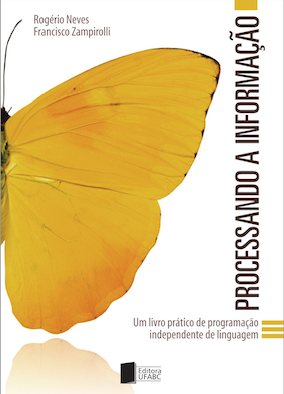
\includegraphics{"figs/Capa_Processando_Informacao.jpg"}

Este caderno (Notebook) é parte complementar \emph{online} do livro
\textbf{\href{https://editora.ufabc.edu.br/matematica-e-ciencias-da-computacao/58-processando-a-informacao}{Processando
a Informação}: um livro prático de programação independente de
linguagem}, que deve ser consultado no caso de dúvidas sobre os temas
apresentados.

\begin{quote}
Este conteúdo pode ser copiado e alterado livremente e foi inspirado
nesse livro.
\end{quote}

    \hypertarget{sumuxe1rio}{%
\subsection{Sumário}\label{sumuxe1rio}}

\begin{itemize}
\tightlist
\item
  Revisão do capítulo anterios
\item
  O que é um desvio condicional?
\item
  Condições com lógica booleana
\item
  Desvios condicionais Simples e Compostos, com Encadeamentos
\item
  Revisão deste capítulo
\item
  Exercícios
\end{itemize}

    \hypertarget{revisuxe3o-do-capuxedtulo-anterior-organizauxe7uxe3o-de-cuxf3digo}{%
\subsection{Revisão do capítulo anterior (Organização de
Código)}\label{revisuxe3o-do-capuxedtulo-anterior-organizauxe7uxe3o-de-cuxf3digo}}

    \begin{itemize}
\item
  No capítulo anterior foram apresentados formas de organização de
  códigos, utilizando comentários, tabulações, escopo de variáveis
  locais e globais, métodos (funções ou procedimentos) e o conceito de
  sistema de informação em partes:

  \begin{itemize}
  \tightlist
  \item
    \textbf{ENTRADA DE DADOS \(\Rightarrow\) PROCESSAMENTO DA INFORMAÇÃO
    \(\Rightarrow\) SAÍDA}
  \end{itemize}
\item
  Neste capítulo serão apresentados códigos com desvios condicionais, da
  forma:

  \begin{itemize}
  \tightlist
  \item
    \texttt{se} algo for verdade, \texttt{então}

    \begin{itemize}
    \tightlist
    \item
      faça algo1,
    \end{itemize}
  \item
    \texttt{senão} \# essa parte é opcional

    \begin{itemize}
    \tightlist
    \item
      faça algo2.
    \end{itemize}
  \end{itemize}
\end{itemize}

    \hypertarget{o-que-uxe9-um-desvio-condional}{%
\subsection{O que é um Desvio
Condional?}\label{o-que-uxe9-um-desvio-condional}}

    \begin{itemize}
\item
  O desvio condicional é a mais simples entre as estruturas lógicas não
  sequenciais em lógica de programação e fundamental para o entendimento
  de fluxo de código.
\item
  A analogia básica com o processo de tomada de decisões ocorre quando
  imaginamos um cenário que proporciona duas possíveis alternativas de
  curso:

  \begin{itemize}
  \tightlist
  \item
    Se {[}condição{]} então faça {[}caminho caso verdadeiro{]} senão
    {[}caminho caso falso{]}
  \end{itemize}
\item
  Exemplos:

  \begin{itemize}
  \tightlist
  \item
    Se {[}está chovendo{]} então {[}resolver palavras cruzadas{]} senão
    {[}andar de bicicleta{]}
  \item
    Se {[}é quarta{]} então {[}comer feijoada{]}
  \end{itemize}
\item
  Ver Fluxograma abaixo (também experimente nessa ferramenta
  \emph{online}: \href{https://app.code2flow.com/}{code2flow}, copiando
  e colando o código em vermelho abaixo):
\end{itemize}

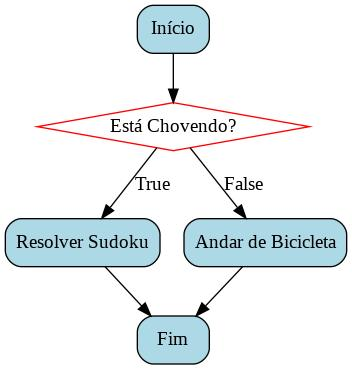
\includegraphics{"figs/flowchartCap3a.jpg"}

    \begin{figure}
\centering
\caption{flowchartCap3a.jpg}
\end{figure}

    \begin{tcolorbox}[breakable, size=fbox, boxrule=1pt, pad at break*=1mm,colback=cellbackground, colframe=cellborder]
\prompt{In}{incolor}{ }{\boxspacing}
\begin{Verbatim}[commandchars=\\\{\}]
\PY{o}{!}apt\PYZhy{}get install graphviz libgraphviz\PYZhy{}dev pkg\PYZhy{}config
\PY{o}{!}pip install txtoflow
\end{Verbatim}
\end{tcolorbox}

    \begin{tcolorbox}[breakable, size=fbox, boxrule=1pt, pad at break*=1mm,colback=cellbackground, colframe=cellborder]
\prompt{In}{incolor}{ }{\boxspacing}
\begin{Verbatim}[commandchars=\\\{\}]
\PY{k+kn}{from} \PY{n+nn}{txtoflow} \PY{k+kn}{import} \PY{n}{txtoflow}

\PY{n}{txtoflow}\PY{o}{.}\PY{n}{generate}\PY{p}{(}
    \PY{l+s+sd}{\PYZsq{}\PYZsq{}\PYZsq{}}
\PY{l+s+sd}{    Início;}
\PY{l+s+sd}{    if (Está Chovendo?) \PYZob{}}
\PY{l+s+sd}{        Resolver Sudoku;}
\PY{l+s+sd}{    \PYZcb{} else \PYZob{}}
\PY{l+s+sd}{        Andar de Bicicleta;}
\PY{l+s+sd}{    \PYZcb{}}
\PY{l+s+sd}{    Fim;}
\PY{l+s+sd}{    \PYZsq{}\PYZsq{}\PYZsq{}}
\PY{p}{)}
\end{Verbatim}
\end{tcolorbox}

    \hypertarget{condiuxe7uxf5es-com-luxf3gica-booleana}{%
\subsection{\texorpdfstring{Condições com Lógica
\emph{Booleana}}{Condições com Lógica Booleana}}\label{condiuxe7uxf5es-com-luxf3gica-booleana}}

    \begin{itemize}
\tightlist
\item
  O resultado de um teste condicional sempre resultará em um valor
  \emph{booleano}, isto é:

  \begin{itemize}
  \tightlist
  \item
    com dois resultados possíveis: \textbf{verdadeiro} ou \textbf{falso}
  \item
    Por convensão: \(True=1\) e \(False=0\)
  \end{itemize}
\item
  Portanto, para condições, sempre usaremos combinações de operadores
  lógicos e relacionais para verificar o estado das variáveis
  verificadas. O seguinte pseudocódigo exemplifica algumas condições:
\end{itemize}

    \begin{verbatim}
se vai chover, então leve um guarda-chuva.

se é feriado, então fique em casa.

se estou atrasado e está chovendo, então chame um taxi.

se minha nota é menor que 5, então fiquei de recuperação.
\end{verbatim}

    \begin{itemize}
\item
  Note que para todas as condições acima, a resposta para a condição é
  sempre: verdadeiro ou falso.
\item
  Caso a condição seja verdadeira, será executada a operação ou
  operações especificadas na sequência.
\item
  Codificando-se, as condições tomam a forma
  \texttt{se\ (condição)\ \{\ comandos\ \}}, como exemplos:
\end{itemize}

    \begin{verbatim}
se (vai_chover) { leve um guarda-chuva }

se (feriado) { fique em casa }

se (atrasado e chovendo) { chame um taxi }

se (nota<5) { escrever “ficou de Recuperação” }
\end{verbatim}

    Esse código anterior \textbf{fica melhor se usar a organização}
apresentada no capítulo anterior:

    \begin{verbatim}
se (vai_chover) 
  leve um guarda-chuva 

se (feriado) 
  fique em casa 

se (atrasado e chovendo)  
  chame um taxi 

se (nota<5) 
  escrever “ficou de Recuperação” 
\end{verbatim}

    \begin{itemize}
\item
  Observe que foram substituídas as chaves \texttt{\{} e \texttt{\}},
  que definem os \textbf{escopos} das condicionais, pela tabulação. Isso
  é possível quando o bloco tem apenas uma instrução.
\item
  Relembrando o Cap. 1 - Fundamentos, podemos usar nas
  \textbf{condicionais}, variáveis \emph{booleanas} e operadores:

  \begin{itemize}
  \tightlist
  \item
    \textbf{relacionais}: ◦ == (é igual a) ◦ != (é diferente de) ◦
    \textgreater{} (é maior que) ◦ \textless{} (é menor que) ◦
    \textgreater= (é maior ou igual a) ◦ \textless= (é menor ou igual a)
  \item
    Além de \textbf{lógicos}: ◦ \&\& (e), \& (e bit-a-bit) ◦
    \textbar\textbar{} (ou), \textbar{} (ou bit a bit) ◦ ! (não lógico
    ou complemento) ◦ \textasciitilde{} (complemento bit-a-bit) ◦ \^{}
    (ou exclusivo `XOR' bit-a-bit) ◦ \textless\textless{} N (shift-left,
    adiciona N zeros à direita do número em binário) ◦
    \textgreater\textgreater{} N (shift-right, elimina N dígitos a
    direita do número em binário)
  \end{itemize}
\end{itemize}

    \begin{itemize}
\item
  Os operadores \textbf{lógicos}, como os \textbf{relacionais}, sempre
  resultarão \textbf{verdadeiro} (V) ou \textbf{falso} (F), porém os
  operandos também são \emph{booleanos}.
\item
  Para as condições contendo AND, OR e XOR (ou exclusivo), as
  \textbf{tabelas verdade} para os dois operandos à esquerda e à
  direita, com valores lógicos representados na primeira linha e
  primeira coluna, são:
\end{itemize}

    \begin{longtable}[]{@{}ccc@{}}
\toprule
\&\& & V & F\tabularnewline
\midrule
\endhead
V & \textbf{V} & F\tabularnewline
F & F & F\tabularnewline
\bottomrule
\end{longtable}

    \begin{longtable}[]{@{}ccc@{}}
\toprule
\textbar\textbar{} & V & F\tabularnewline
\midrule
\endhead
V & V & V\tabularnewline
F & V & \textbf{F}\tabularnewline
\bottomrule
\end{longtable}

    \begin{longtable}[]{@{}ccc@{}}
\toprule
\^{} & V & F\tabularnewline
\midrule
\endhead
V & F & V\tabularnewline
F & V & F\tabularnewline
\bottomrule
\end{longtable}

    \begin{itemize}
\tightlist
\item
  Logo,

  \begin{itemize}
  \tightlist
  \item
    os operandos devem ser ambos verdadeiros para que a operação AND
    retorne verdadeiro,
  \item
    ao menos um deles verdadeiro para que o OR retorne verdadeiro e
  \item
    ambos diferentes para que o XOR (ou exclusivo \texttt{\^{}}) retorne
    verdadeiro.
  \end{itemize}
\end{itemize}

    \begin{itemize}
\item
  Estas expressões, quando combinadas, resultarão sempre em um valor
  \emph{booleano} V ou F, que pode ser então introduzido em um desvio
  condicional visando à realização de um subprograma.
\item
  Por exemplo, usando os valores X=1, Y=2 e Z=4, qual o resultado das
  expressões abaixo?
\end{itemize}

\begin{quote}
\begin{enumerate}
\def\labelenumi{\arabic{enumi}.}
\tightlist
\item
  (X\textgreater0 \&\& Y\textless2)
\item
  (Z\textgreater0 \textbar\textbar{} Z\textless5 \&\& Y==4)
\item
  (X\textgreater\textgreater1 ==0 \textbar\textbar{}
  Y\textless\textless2\textgreater100)
\item
  (X!=0 \&\& Y!=0 \&\& Z\textless0)
\item
  (X=1)
\end{enumerate}
\end{quote}

    \begin{itemize}
\tightlist
\item
  Dada a precedência de operadores estudada anteriormente e a combinação
  apresentada acima, apenas as expressões 2 e 3 resultariam em
  verdadeiro, dado \(Z>0\), assim como \(1>>1\) (\emph{shift} à direita
  uma casa) em binário é 0; são ambas condições suficientes para que o
  resultado seja verdadeiro.
\end{itemize}

    \begin{tcolorbox}[breakable, size=fbox, boxrule=1pt, pad at break*=1mm,colback=cellbackground, colframe=cellborder]
\prompt{In}{incolor}{ }{\boxspacing}
\begin{Verbatim}[commandchars=\\\{\}]
\PY{n}{X}\PY{p}{,} \PY{n}{Y}\PY{p}{,} \PY{n}{Z} \PY{o}{=}\PY{l+m+mi}{1}\PY{p}{,} \PY{l+m+mi}{2}\PY{p}{,} \PY{l+m+mi}{4}
\PY{n}{equacao1} \PY{o}{=} \PY{p}{(}\PY{n}{X}\PY{o}{\PYZgt{}}\PY{l+m+mi}{0} \PY{o+ow}{and} \PY{n}{Y}\PY{o}{\PYZlt{}}\PY{l+m+mi}{2}\PY{p}{)}
\PY{n}{equacao2} \PY{o}{=} \PY{p}{(}\PY{n}{Z}\PY{o}{\PYZgt{}}\PY{l+m+mi}{0} \PY{o+ow}{or} \PY{n}{Z}\PY{o}{\PYZlt{}}\PY{l+m+mi}{5} \PY{o+ow}{and} \PY{n}{Y}\PY{o}{==}\PY{l+m+mi}{4}\PY{p}{)}
\PY{n}{equacao3} \PY{o}{=} \PY{p}{(}\PY{n}{X}\PY{o}{\PYZgt{}\PYZgt{}}\PY{l+m+mi}{1} \PY{o}{==}\PY{l+m+mi}{0} \PY{o+ow}{or} \PY{n}{Y}\PY{o}{\PYZlt{}\PYZlt{}}\PY{l+m+mi}{2}\PY{o}{\PYZgt{}}\PY{l+m+mi}{100}\PY{p}{)}
\PY{n}{equacao4} \PY{o}{=} \PY{p}{(}\PY{n}{X}\PY{o}{!=}\PY{l+m+mi}{0} \PY{o+ow}{and} \PY{n}{Y}\PY{o}{!=}\PY{l+m+mi}{0} \PY{o+ow}{and} \PY{n}{Z}\PY{o}{\PYZlt{}}\PY{l+m+mi}{0}\PY{p}{)}
\PY{c+c1}{\PYZsh{}equacao5 = (X=1) \PYZsh{} ERRO de sintaxe, deveria ser X==1}
\PY{n+nb}{print}\PY{p}{(}\PY{n}{equacao1}\PY{p}{,}\PY{n}{equacao2}\PY{p}{,}\PY{n}{equacao3}\PY{p}{,}\PY{n}{equacao4}\PY{p}{)}
\end{Verbatim}
\end{tcolorbox}

    \begin{tcolorbox}[breakable, size=fbox, boxrule=1pt, pad at break*=1mm,colback=cellbackground, colframe=cellborder]
\prompt{In}{incolor}{ }{\boxspacing}
\begin{Verbatim}[commandchars=\\\{\}]
\PY{c+c1}{\PYZsh{} exemplo de uso de \PYZdq{}\PYZgt{}\PYZgt{}\PYZdq{} }
\PY{c+c1}{\PYZsh{} 6 = 1 1 0 em binário =\PYZgt{} 1*2\PYZca{}2 + 1*2\PYZca{}1 + 0*2\PYZca{}0}
\PY{l+m+mi}{6}\PY{o}{\PYZgt{}\PYZgt{}}\PY{l+m+mi}{1} \PY{c+c1}{\PYZsh{} = 3 = 0 1 1 em binário}
\end{Verbatim}
\end{tcolorbox}

    \begin{itemize}
\tightlist
\item
  É importante ressaltar a diferença entre os operadores de comparação
  \texttt{==}, com leitura \texttt{é\ igual\ à}, e de atribuição
  \texttt{=}, tendo a leitura \texttt{recebe\ o\ valor\ de}. Neste
  aspecto, a expressão 5 está incorreta, já que o operador de atribuição
  não faz sentido quando usado desta forma.
\end{itemize}

    \hypertarget{desvios-condicionais-simples-e-compostos}{%
\subsection{Desvios Condicionais Simples e
Compostos}\label{desvios-condicionais-simples-e-compostos}}

    \begin{verbatim}
se (condição) então faça 
    Comandos

Volta para a parte sequencial
\end{verbatim}

\begin{verbatim}
se (condição) então faça 
    Comandos
senão faça 
    Comandos

Volta para a parte sequencial
\end{verbatim}

    \begin{verbatim}
if (condição) {
    Comandos
}
\end{verbatim}

\begin{verbatim}
if (condição) {
    Comandos
} else {
    Comandos
}
\end{verbatim}

    \hypertarget{exemplo-01---uso-de-condicionais-simples}{%
\paragraph{Exemplo 01 - Uso de Condicionais
Simples}\label{exemplo-01---uso-de-condicionais-simples}}

    \begin{itemize}
\item
  Digamos que, como exemplo, desejamos calcular as raízes da equação de
  segundo grau usando a função \texttt{delta()} introduzida no capítulo
  anterior.
\item
  Sabemos que as raízes dependem do sinal do \(\Delta\).
\item
  Logo, a solução de uma equação do segundo grau se dá resolvendo as
  seguintes condições:
\end{itemize}

\begin{quote}
\begin{enumerate}
\def\labelenumi{\arabic{enumi}.}
\tightlist
\item
  Se \(\Delta<0\), \(x\) não possui raízes reais;
\item
  Se \(\Delta=0\), \(x\) possui duas raízes reais idênticas;
\item
  Se \(\Delta>0\), \(x\) possui duas raízes reais e distintas;
\item
  Calcule as raízes, se existirem, usando as equações:
\end{enumerate}
\end{quote}

\[x1 = -b+\frac{\sqrt{\Delta}}{2a}\]

\[x2 = -b-\frac{\sqrt{\Delta}}{2a}\]

\begin{itemize}
\tightlist
\item
  Veja uma solução em pseudocódigo:
\end{itemize}

    \begin{verbatim}
# a função é definida a seguir
função delta(a, b, c )
  retorne b * b - 4 * a * c
 
# programa principal  
# ENTRADA DE DADOS
escreva("Calcula as raízes de equação de 2º grau: ax2 + bx + c")
real a = leia("Entre com o primeiro termo ‘a’: ")
real b = leia("Entre com o segundo  termo ‘b’: ") 
real c = leia("Entre com o terceiro termo ‘c’: ") 
 
# PROCESSAMENTO E SAÍDA
real d = delta(5, -2, 4)
escreva(“O delta é ” + valor)
se (d < 0)  
  escreva("A equação não possui raízes reais")
se (d == 0) 
  escreva("A raíz é " + (-b + raíz(d)/2*a))
se (d > 0)  
  escreva("As raízes são x1=" + (-b - raíz(d)/2*a)) + " e x2="  + 
  (-b + raíz(d)/2*a))
\end{verbatim}

    Casos para Teste Moodle+VPL

Para o professor criar uma atividade VPL no Moodle para este Exemplo 01,
basta incluir em \texttt{Casos\ para\ teste}, o seguinte texto (pode
incluir mais casos):

\begin{verbatim}
case=caso1
input=3
1
4
output= 
O delta é  -47.0
A equação não possui raízes reais.
case=caso2
input=4
6
2
output= O delta é 4.0
Raízes: -10.0 e -2.0.
\end{verbatim}

    \begin{tcolorbox}[breakable, size=fbox, boxrule=1pt, pad at break*=1mm,colback=cellbackground, colframe=cellborder]
\prompt{In}{incolor}{ }{\boxspacing}
\begin{Verbatim}[commandchars=\\\{\}]
\PY{o}{\PYZpc{}\PYZpc{}writefile} cap3ex01.c
\PY{c+c1}{\PYZsh{}include \PYZlt{}stdio.h\PYZgt{}}
\PY{c+c1}{\PYZsh{}include \PYZlt{}math.h\PYZgt{}}
\PY{n+nb}{float} \PY{n}{delta}\PY{p}{(}\PY{n+nb}{float} \PY{n}{a}\PY{p}{,} \PY{n+nb}{float} \PY{n}{b}\PY{p}{,} \PY{n+nb}{float} \PY{n}{c}\PY{p}{)} \PY{p}{\PYZob{}}
  \PY{n+nb}{float} \PY{n}{d} \PY{o}{=} \PY{n}{b}\PY{o}{*}\PY{n}{b}\PY{o}{\PYZhy{}}\PY{l+m+mi}{4}\PY{o}{*}\PY{n}{a}\PY{o}{*}\PY{n}{c}\PY{p}{;}
  \PY{k}{return} \PY{n}{d}\PY{p}{;}
\PY{p}{\PYZcb{}}

\PY{n+nb}{float} \PY{n}{leia}\PY{p}{(}\PY{p}{)} \PY{p}{\PYZob{}}
  \PY{n+nb}{float} \PY{n}{valor}\PY{p}{;}
  \PY{n}{printf}\PY{p}{(}\PY{l+s+s2}{\PYZdq{}}\PY{l+s+s2}{Entre com um valor: }\PY{l+s+s2}{\PYZdq{}}\PY{p}{)}\PY{p}{;}
  \PY{n}{scanf}\PY{p}{(}\PY{l+s+s2}{\PYZdq{}}\PY{l+s+si}{\PYZpc{}f}\PY{l+s+s2}{\PYZdq{}}\PY{p}{,} \PY{o}{\PYZam{}}\PY{n}{valor}\PY{p}{)}\PY{p}{;}
  \PY{k}{return} \PY{n}{valor}\PY{p}{;}
\PY{p}{\PYZcb{}}

\PY{n+nb}{int} \PY{n}{main}\PY{p}{(}\PY{n}{void}\PY{p}{)} \PY{p}{\PYZob{}}

  \PY{o}{/}\PY{o}{/} \PY{n}{ENTRADAS}
  \PY{n+nb}{float} \PY{n}{a}\PY{p}{,} \PY{n}{b}\PY{p}{,} \PY{n}{c}\PY{p}{;}
  \PY{n}{a} \PY{o}{=} \PY{n}{leia}\PY{p}{(}\PY{p}{)}\PY{p}{;}
  \PY{n}{b} \PY{o}{=} \PY{n}{leia}\PY{p}{(}\PY{p}{)}\PY{p}{;}
  \PY{n}{c} \PY{o}{=} \PY{n}{leia}\PY{p}{(}\PY{p}{)}\PY{p}{;}
  
  \PY{o}{/}\PY{o}{/} \PY{n}{PROCESSAMENTO} \PY{n}{e} \PY{n}{SAÍDA}
  \PY{n}{double} \PY{n}{d} \PY{o}{=} \PY{p}{(}\PY{n}{double}\PY{p}{)} \PY{n}{delta}\PY{p}{(}\PY{n}{a}\PY{p}{,} \PY{n}{b}\PY{p}{,} \PY{n}{c}\PY{p}{)}\PY{p}{;}
  \PY{n}{printf}\PY{p}{(}\PY{l+s+s2}{\PYZdq{}}\PY{l+s+s2}{Delta = }\PY{l+s+si}{\PYZpc{}.1f}\PY{l+s+se}{\PYZbs{}n}\PY{l+s+s2}{\PYZdq{}}\PY{p}{,} \PY{n}{d}\PY{p}{)}\PY{p}{;}
  \PY{k}{if} \PY{p}{(}\PY{n}{d} \PY{o}{\PYZlt{}} \PY{l+m+mi}{0}\PY{p}{)} \PY{p}{\PYZob{}}
      \PY{n}{printf}\PY{p}{(}\PY{l+s+s2}{\PYZdq{}}\PY{l+s+s2}{A equação não possui raízes reais}\PY{l+s+s2}{\PYZdq{}}\PY{p}{)}\PY{p}{;}
  \PY{p}{\PYZcb{}}
  \PY{k}{if} \PY{p}{(}\PY{n}{d} \PY{o}{==} \PY{l+m+mi}{0}\PY{p}{)} \PY{p}{\PYZob{}}
      \PY{n}{printf}\PY{p}{(}\PY{l+s+s2}{\PYZdq{}}\PY{l+s+s2}{Raíz: }\PY{l+s+si}{\PYZpc{}.1f}\PY{l+s+s2}{\PYZdq{}}\PY{p}{,}\PY{p}{(}\PY{o}{\PYZhy{}}\PY{n}{b} \PY{o}{+} \PY{n}{sqrt}\PY{p}{(}\PY{n}{d}\PY{p}{)} \PY{o}{/} \PY{l+m+mi}{2} \PY{o}{*} \PY{n}{a}\PY{p}{)}\PY{p}{)}\PY{p}{;}
  \PY{p}{\PYZcb{}}
  \PY{k}{if} \PY{p}{(}\PY{n}{d} \PY{o}{\PYZgt{}} \PY{l+m+mi}{0}\PY{p}{)} \PY{p}{\PYZob{}}
      \PY{n}{printf}\PY{p}{(}\PY{l+s+s2}{\PYZdq{}}\PY{l+s+s2}{Raíz: }\PY{l+s+si}{\PYZpc{}.1f}\PY{l+s+s2}{ e }\PY{l+s+si}{\PYZpc{}.1f}\PY{l+s+s2}{ }\PY{l+s+s2}{\PYZdq{}}\PY{p}{,}\PY{p}{(}\PY{o}{\PYZhy{}}\PY{n}{b} \PY{o}{\PYZhy{}} \PY{n}{sqrt}\PY{p}{(}\PY{n}{d}\PY{p}{)} \PY{o}{/} \PY{l+m+mi}{2} \PY{o}{*} \PY{n}{a}\PY{p}{)}\PY{p}{,} \PY{p}{(}\PY{o}{\PYZhy{}}\PY{n}{b} \PY{o}{+} \PY{n}{sqrt}\PY{p}{(}\PY{n}{d}\PY{p}{)} \PY{o}{/} \PY{l+m+mi}{2} \PY{o}{*} \PY{n}{a}\PY{p}{)}\PY{p}{)}\PY{p}{;}
  \PY{p}{\PYZcb{}}
  \PY{k}{return} \PY{l+m+mi}{0}\PY{p}{;}
\PY{p}{\PYZcb{}}
\end{Verbatim}
\end{tcolorbox}

    \begin{tcolorbox}[breakable, size=fbox, boxrule=1pt, pad at break*=1mm,colback=cellbackground, colframe=cellborder]
\prompt{In}{incolor}{ }{\boxspacing}
\begin{Verbatim}[commandchars=\\\{\}]
\PY{o}{\PYZpc{}\PYZpc{}}\PY{k}{shell}
gcc \PYZhy{}Wall \PYZhy{}std=c99 cap3ex01.c \PYZhy{}o output2 \PYZhy{}lm
./output2
\PYZsh{} A biblioteca matemática deve ser vinculada ao construir o executável. 
\PYZsh{} Como fazer isso varia de acordo com o ambiente, 
\PYZsh{} mas no Linux / Unix, basta adicionar \PYZhy{}lm ao comando
\end{Verbatim}
\end{tcolorbox}

    \hypertarget{exemplo-02---uso-de-condicionais-compostas-e-encadeadas}{%
\paragraph{Exemplo 02 - Uso de Condicionais Compostas e
Encadeadas}\label{exemplo-02---uso-de-condicionais-compostas-e-encadeadas}}

    \begin{itemize}
\tightlist
\item
  Considere o seguinte pseudocódigo para ler duas notas reais, calcular
  a média das duas notas e atribui um conceito:
\end{itemize}

    \begin{verbatim}
nota1 = leia("Digite a 1a nota:");
nota2 = leia("Digite a 2a nota:");
media = (nota1 + nota2)/2;
se media >= 9 então  
    escreva("Conceito A"); 
senão se media >= 7.5  
    escreva("Conceito B"); 
senão se media >= 6 
    escreva("Conceito C"); 
senão se media >= 5| 
    escreva("Conceito D"); 
senão 
    escreva("Reprovado! Conceito F"); 
\end{verbatim}

    \begin{itemize}
\tightlist
\item
  Ver Fluxograma abaixo (também experimente nessa ferramenta
  \emph{online}: \href{https://app.code2flow.com/}{code2flow}, copiando
  e colando o código em vermelho abaixo):
\end{itemize}

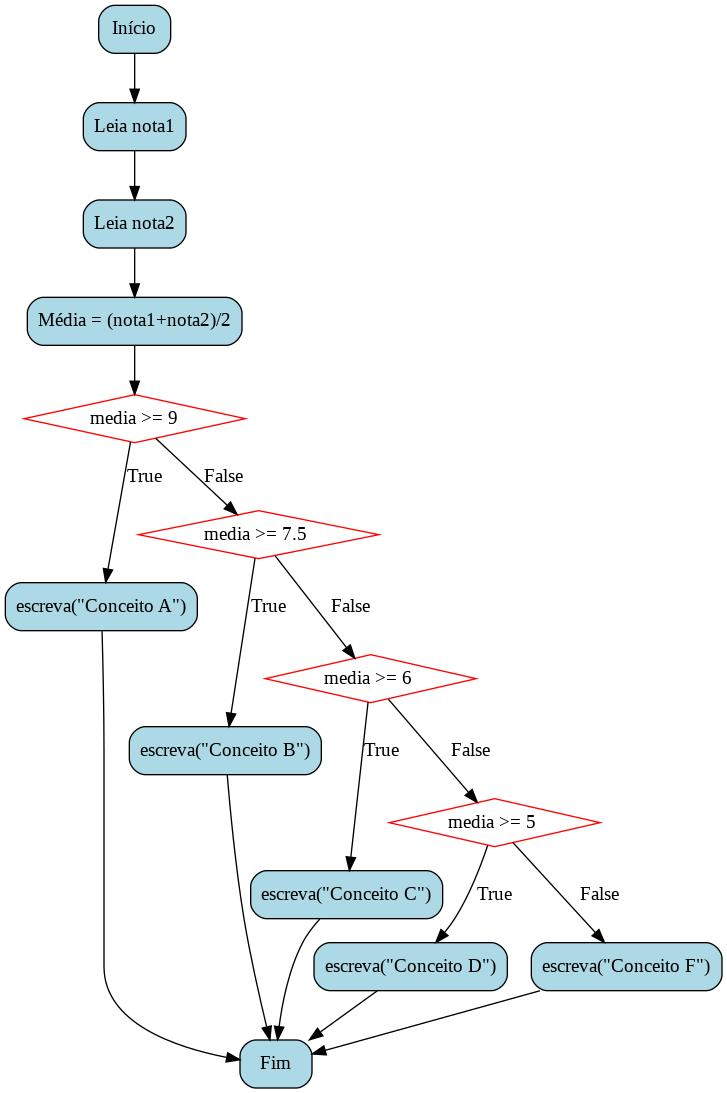
\includegraphics{"figs/flowchartCap3b.jpg"}

    \begin{figure}
\centering
\caption{flowchartCap3b.jpg}
\end{figure}

    \begin{tcolorbox}[breakable, size=fbox, boxrule=1pt, pad at break*=1mm,colback=cellbackground, colframe=cellborder]
\prompt{In}{incolor}{ }{\boxspacing}
\begin{Verbatim}[commandchars=\\\{\}]
\PY{k+kn}{from} \PY{n+nn}{txtoflow} \PY{k+kn}{import} \PY{n}{txtoflow}

\PY{n}{txtoflow}\PY{o}{.}\PY{n}{generate}\PY{p}{(}
    \PY{l+s+sd}{\PYZsq{}\PYZsq{}\PYZsq{}}
\PY{l+s+sd}{    Início;}
\PY{l+s+sd}{    Leia nota1;}
\PY{l+s+sd}{    Leia nota2;}
\PY{l+s+sd}{    Média = (nota1+nota2)/2;}
\PY{l+s+sd}{    if ( media \PYZgt{}= 9 ) \PYZob{}}
\PY{l+s+sd}{        escreva(\PYZdq{}Conceito A\PYZdq{}); }
\PY{l+s+sd}{    \PYZcb{} else if (media \PYZgt{}= 7.5 ) \PYZob{}}
\PY{l+s+sd}{        escreva(\PYZdq{}Conceito B\PYZdq{}); }
\PY{l+s+sd}{    \PYZcb{} else if (media \PYZgt{}= 6 ) \PYZob{}}
\PY{l+s+sd}{        escreva(\PYZdq{}Conceito C\PYZdq{}); }
\PY{l+s+sd}{    \PYZcb{} else if (media \PYZgt{}= 5 ) \PYZob{}}
\PY{l+s+sd}{        escreva(\PYZdq{}Conceito D\PYZdq{}); }
\PY{l+s+sd}{    \PYZcb{} else \PYZob{}}
\PY{l+s+sd}{        escreva(\PYZdq{}Conceito F\PYZdq{}); }
\PY{l+s+sd}{    \PYZcb{}}
\PY{l+s+sd}{    Fim;}
\PY{l+s+sd}{    \PYZsq{}\PYZsq{}\PYZsq{}}
\PY{p}{)}
\end{Verbatim}
\end{tcolorbox}

    Casos para Teste Moodle+VPL

Para o professor criar uma atividade VPL no Moodle para este Exemplo 02,
basta incluir em \texttt{Casos\ para\ teste}, o seguinte texto (pode
incluir mais casos):

\begin{verbatim}
case=caso1
input=4.0
6.0
output= 
Conceito D
case=caso2
input=4.0
5.0
output= 
Conceito F
case=caso2
input=5.0
7.0
output= 
Conceito C
case=caso3
input=6.0
9.0
output= 
Conceito B
case=caso4
input=9.0
10.0
output= 
Conceito A
\end{verbatim}

    \begin{tcolorbox}[breakable, size=fbox, boxrule=1pt, pad at break*=1mm,colback=cellbackground, colframe=cellborder]
\prompt{In}{incolor}{ }{\boxspacing}
\begin{Verbatim}[commandchars=\\\{\}]
\PY{o}{\PYZpc{}\PYZpc{}writefile} cap3ex02.c
\PY{c+c1}{\PYZsh{}include \PYZlt{}stdio.h\PYZgt{}}
\PY{n+nb}{float} \PY{n}{leia}\PY{p}{(}\PY{p}{)} \PY{p}{\PYZob{}}
  \PY{n+nb}{float} \PY{n}{valor}\PY{p}{;}
  \PY{n}{printf}\PY{p}{(}\PY{l+s+s2}{\PYZdq{}}\PY{l+s+s2}{Entre com um valor: }\PY{l+s+s2}{\PYZdq{}}\PY{p}{)}\PY{p}{;}
  \PY{n}{scanf}\PY{p}{(}\PY{l+s+s2}{\PYZdq{}}\PY{l+s+si}{\PYZpc{}f}\PY{l+s+s2}{\PYZdq{}}\PY{p}{,} \PY{o}{\PYZam{}}\PY{n}{valor}\PY{p}{)}\PY{p}{;}
  \PY{k}{return} \PY{n}{valor}\PY{p}{;}
\PY{p}{\PYZcb{}}

\PY{n+nb}{int} \PY{n}{main}\PY{p}{(}\PY{n}{void}\PY{p}{)} \PY{p}{\PYZob{}}

  \PY{o}{/}\PY{o}{/} \PY{n}{ENTRADAS}
  \PY{n+nb}{float} \PY{n}{nota1} \PY{o}{=} \PY{n}{leia}\PY{p}{(}\PY{p}{)}\PY{p}{;}
  \PY{n+nb}{float} \PY{n}{nota2} \PY{o}{=} \PY{n}{leia}\PY{p}{(}\PY{p}{)}\PY{p}{;}

  \PY{o}{/}\PY{o}{/} \PY{n}{PROCESSAMENTO} \PY{n}{E} \PY{n}{SAÍDA}
  \PY{n+nb}{float} \PY{n}{media} \PY{o}{=} \PY{p}{(}\PY{n}{nota1} \PY{o}{+} \PY{n}{nota2}\PY{p}{)}\PY{o}{/}\PY{l+m+mi}{2}\PY{p}{;}
  \PY{k}{if} \PY{p}{(}\PY{n}{media} \PY{o}{\PYZgt{}}\PY{o}{=} \PY{l+m+mf}{9.0}\PY{p}{)}      
    \PY{n}{printf}\PY{p}{(}\PY{l+s+s2}{\PYZdq{}}\PY{l+s+s2}{Conceito A}\PY{l+s+s2}{\PYZdq{}}\PY{p}{)}\PY{p}{;} 
  \PY{k}{else} \PY{k}{if} \PY{p}{(}\PY{n}{media} \PY{o}{\PYZgt{}}\PY{o}{=} \PY{l+m+mf}{7.5}\PY{p}{)} 
    \PY{n}{printf}\PY{p}{(}\PY{l+s+s2}{\PYZdq{}}\PY{l+s+s2}{Conceito B}\PY{l+s+s2}{\PYZdq{}}\PY{p}{)}\PY{p}{;}
  \PY{k}{else} \PY{k}{if} \PY{p}{(}\PY{n}{media} \PY{o}{\PYZgt{}}\PY{o}{=} \PY{l+m+mf}{6.0}\PY{p}{)} 
    \PY{n}{printf}\PY{p}{(}\PY{l+s+s2}{\PYZdq{}}\PY{l+s+s2}{Conceito C}\PY{l+s+s2}{\PYZdq{}}\PY{p}{)}\PY{p}{;}
  \PY{k}{else} \PY{k}{if} \PY{p}{(}\PY{n}{media} \PY{o}{\PYZgt{}}\PY{o}{=} \PY{l+m+mf}{5.0}\PY{p}{)} 
    \PY{n}{printf}\PY{p}{(}\PY{l+s+s2}{\PYZdq{}}\PY{l+s+s2}{Conceito D}\PY{l+s+s2}{\PYZdq{}}\PY{p}{)}\PY{p}{;}
  \PY{k}{else}        
    \PY{n}{printf}\PY{p}{(}\PY{l+s+s2}{\PYZdq{}}\PY{l+s+s2}{Reprovado! Conceito F.}\PY{l+s+s2}{\PYZdq{}}\PY{p}{)}\PY{p}{;}
  \PY{k}{return} \PY{l+m+mi}{0}\PY{p}{;}
\PY{p}{\PYZcb{}}
\end{Verbatim}
\end{tcolorbox}

    \begin{tcolorbox}[breakable, size=fbox, boxrule=1pt, pad at break*=1mm,colback=cellbackground, colframe=cellborder]
\prompt{In}{incolor}{ }{\boxspacing}
\begin{Verbatim}[commandchars=\\\{\}]
\PY{o}{\PYZpc{}\PYZpc{}}\PY{k}{shell}
gcc \PYZhy{}Wall \PYZhy{}std=c99 cap3ex02.c \PYZhy{}o output2
./output2
\end{Verbatim}
\end{tcolorbox}

    \hypertarget{comando-switch}{%
\subsection{\texorpdfstring{Comando
\texttt{switch}}{Comando switch}}\label{comando-switch}}

    O \texttt{switch} verifica se uma variável (do tipo \texttt{int} ou
\texttt{char}) é ou não igual a certo valor constante (valor1, valor2,
\ldots, valorN na sintaxe a seguir):

\begin{verbatim}
switch (variável) {
  case valor1:
    Comandos;
    break;
  case valor2:
    Comandos;
    break;
  case valorN:
    Comandos;
    break;
  default: // opcional, caso não ocorram os casos anteriores
    Comandos;
}
\end{verbatim}

Esse comanto \texttt{switch} é útil quando se tem um menu de opções a
ser executado.

    \hypertarget{exemplo-03---exemplo-de-switch-com-menu-de-opuxe7uxf5es}{%
\paragraph{\texorpdfstring{Exemplo 03 - Exemplo de \texttt{switch} com
menu de
opções}{Exemplo 03 - Exemplo de switch com menu de opções}}\label{exemplo-03---exemplo-de-switch-com-menu-de-opuxe7uxf5es}}

    \begin{tcolorbox}[breakable, size=fbox, boxrule=1pt, pad at break*=1mm,colback=cellbackground, colframe=cellborder]
\prompt{In}{incolor}{1}{\boxspacing}
\begin{Verbatim}[commandchars=\\\{\}]
\PY{o}{\PYZpc{}\PYZpc{}writefile} cap3ex03.c
\PY{c+c1}{\PYZsh{}include \PYZlt{}stdio.h\PYZgt{}}
\PY{n+nb}{int} \PY{n}{main}\PY{p}{(}\PY{p}{)} \PY{p}{\PYZob{}}
  \PY{n+nb}{float} \PY{n}{area}\PY{p}{;}
  \PY{n+nb}{int} \PY{n}{num}\PY{p}{;}
  \PY{n}{char} \PY{n}{escolha}\PY{p}{;}
  \PY{n}{printf}\PY{p}{(}\PY{l+s+s2}{\PYZdq{}}\PY{l+s+s2}{1. Circulo}\PY{l+s+se}{\PYZbs{}n}\PY{l+s+s2}{\PYZdq{}}\PY{p}{)}\PY{p}{;}
  \PY{n}{printf}\PY{p}{(}\PY{l+s+s2}{\PYZdq{}}\PY{l+s+s2}{2. Quadrado}\PY{l+s+se}{\PYZbs{}n}\PY{l+s+s2}{\PYZdq{}}\PY{p}{)}\PY{p}{;}
  \PY{n}{printf}\PY{p}{(}\PY{l+s+s2}{\PYZdq{}}\PY{l+s+s2}{Escolha:}\PY{l+s+se}{\PYZbs{}n}\PY{l+s+s2}{\PYZdq{}}\PY{p}{)}\PY{p}{;}

  \PY{n}{scanf}\PY{p}{(}\PY{l+s+s2}{\PYZdq{}}\PY{l+s+si}{\PYZpc{}c}\PY{l+s+s2}{\PYZdq{}}\PY{p}{,} \PY{o}{\PYZam{}}\PY{n}{escolha}\PY{p}{)}\PY{p}{;}

  \PY{n}{switch} \PY{p}{(}\PY{n}{escolha}\PY{p}{)} \PY{p}{\PYZob{}}
  \PY{k}{case} \PY{l+s+s1}{\PYZsq{}}\PY{l+s+s1}{1}\PY{l+s+s1}{\PYZsq{}}\PY{p}{:}
    \PY{n}{printf}\PY{p}{(}\PY{l+s+s2}{\PYZdq{}}\PY{l+s+s2}{Raio:}\PY{l+s+se}{\PYZbs{}n}\PY{l+s+s2}{\PYZdq{}}\PY{p}{)}\PY{p}{;}
    \PY{n}{scanf}\PY{p}{(}\PY{l+s+s2}{\PYZdq{}}\PY{l+s+si}{\PYZpc{}d}\PY{l+s+s2}{\PYZdq{}}\PY{p}{,} \PY{o}{\PYZam{}}\PY{n}{num}\PY{p}{)}\PY{p}{;}
    \PY{n}{area} \PY{o}{=} \PY{l+m+mf}{3.14} \PY{o}{*} \PY{n}{num} \PY{o}{*} \PY{n}{num}\PY{p}{;}
    \PY{n}{printf}\PY{p}{(}\PY{l+s+s2}{\PYZdq{}}\PY{l+s+s2}{Area do circulo: }\PY{l+s+s2}{\PYZdq{}}\PY{p}{)}\PY{p}{;}
    \PY{n}{printf}\PY{p}{(}\PY{l+s+s2}{\PYZdq{}}\PY{l+s+si}{\PYZpc{}.2f}\PY{l+s+se}{\PYZbs{}n}\PY{l+s+s2}{\PYZdq{}}\PY{p}{,} \PY{n}{area}\PY{p}{)}\PY{p}{;}
    \PY{k}{break}\PY{p}{;}

  \PY{k}{case} \PY{l+s+s1}{\PYZsq{}}\PY{l+s+s1}{2}\PY{l+s+s1}{\PYZsq{}}\PY{p}{:}
    \PY{n}{printf}\PY{p}{(}\PY{l+s+s2}{\PYZdq{}}\PY{l+s+s2}{Lado:}\PY{l+s+se}{\PYZbs{}n}\PY{l+s+s2}{\PYZdq{}}\PY{p}{)}\PY{p}{;}
    \PY{n}{scanf}\PY{p}{(}\PY{l+s+s2}{\PYZdq{}}\PY{l+s+si}{\PYZpc{}d}\PY{l+s+s2}{\PYZdq{}}\PY{p}{,} \PY{o}{\PYZam{}}\PY{n}{num}\PY{p}{)}\PY{p}{;}
    \PY{n}{area} \PY{o}{=} \PY{n}{num} \PY{o}{*} \PY{n}{num}\PY{p}{;}
    \PY{n}{printf}\PY{p}{(}\PY{l+s+s2}{\PYZdq{}}\PY{l+s+s2}{Area do quadrado: }\PY{l+s+s2}{\PYZdq{}}\PY{p}{)}\PY{p}{;}
    \PY{n}{printf}\PY{p}{(}\PY{l+s+s2}{\PYZdq{}}\PY{l+s+si}{\PYZpc{}.2f}\PY{l+s+se}{\PYZbs{}n}\PY{l+s+s2}{\PYZdq{}}\PY{p}{,} \PY{n}{area}\PY{p}{)}\PY{p}{;}
    \PY{k}{break}\PY{p}{;}

  \PY{n}{default}\PY{p}{:}
    \PY{n}{printf}\PY{p}{(}\PY{l+s+s2}{\PYZdq{}}\PY{l+s+s2}{Escolha Incorreta!}\PY{l+s+se}{\PYZbs{}n}\PY{l+s+s2}{\PYZdq{}}\PY{p}{)}\PY{p}{;}
  \PY{p}{\PYZcb{}}
  \PY{k}{return} \PY{l+m+mi}{0}\PY{p}{;}
\PY{p}{\PYZcb{}}
\end{Verbatim}
\end{tcolorbox}

    \begin{tcolorbox}[breakable, size=fbox, boxrule=1pt, pad at break*=1mm,colback=cellbackground, colframe=cellborder]
\prompt{In}{incolor}{3}{\boxspacing}
\begin{Verbatim}[commandchars=\\\{\}]
\PY{o}{\PYZpc{}\PYZpc{}}\PY{k}{shell}
gcc \PYZhy{}Wall \PYZhy{}std=c99 cap3ex03.c \PYZhy{}o output3
./output3
\end{Verbatim}
\end{tcolorbox}

    \hypertarget{exercuxedcios}{%
\subsection{Exercícios}\label{exercuxedcios}}

    Ver notebook Colab no arquivo \texttt{cap3.part2.lab.*.ipynb}
(\texttt{*} é a extensão da linguagem), utilizando aluma linguagem de
programação de sua preferência, onganizadas em subpastas contidas de
\texttt{"gen"}, na pasta do Google Drive
\href{https://drive.google.com/drive/folders/1YlFwv8XYN7PYYf-HwDMlkxzbmXzJw9cM?usp=sharing}{colabs}.

    \hypertarget{revisuxe3o-deste-capuxedtulo-de-desvios-condicionais}{%
\subsection{Revisão deste capítulo de Desvios
Condicionais}\label{revisuxe3o-deste-capuxedtulo-de-desvios-condicionais}}

\begin{itemize}
\tightlist
\item
  O que é um desvio condicional?
\item
  Condições com lógica booleana
\item
  Desvios condicionais Simples e Compostos, com Encadeamentos
\item
  Exercícios
\item
  Revisão deste capítulo de Desvios Condicionais
\end{itemize}

    \hypertarget{processando-a-informauxe7uxe3o-cap.-3-desvios-condicionais---pruxe1tica-1}{%
\subsection{Processando a Informação: Cap. 3: Desvios Condicionais -
Prática
1}\label{processando-a-informauxe7uxe3o-cap.-3-desvios-condicionais---pruxe1tica-1}}

    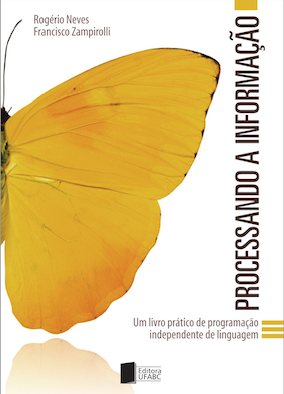
\includegraphics{"figs/Capa_Processando_Informacao.jpg"}

Este caderno (Notebook) é parte complementar \emph{online} do livro
\textbf{\href{https://editora.ufabc.edu.br/matematica-e-ciencias-da-computacao/58-processando-a-informacao}{Processando
a Informação}: um livro prático de programação independente de
linguagem}, que deve ser consultado no caso de dúvidas sobre os temas
apresentados.

\begin{quote}
Este conteúdo pode ser copiado e alterado livremente e foi inspirado
nesse livro.
\end{quote}

    \hypertarget{exercuxedcios}{%
\subsubsection{Exercícios}\label{exercuxedcios}}

    \begin{center}\rule{0.5\linewidth}{0.5pt}\end{center}

\begin{enumerate}
\def\labelenumi{\arabic{enumi}.}
\tightlist
\item
  Crie um método com apenas condicionais e o operador resto (\%) para:
\end{enumerate}

\begin{itemize}
\tightlist
\item
  Determinar se um número entrado pelo teclado é par ou ímpar, exibindo
  a mensagem apropriada na tela;\\
\item
  Modifique o método anterior para verificar se o número entrado é
  múltiplo de 3.
\end{itemize}

Teste em um programa principal várias chamadas destes métodos.

    \begin{center}\rule{0.5\linewidth}{0.5pt}\end{center}

\begin{enumerate}
\def\labelenumi{\arabic{enumi}.}
\setcounter{enumi}{1}
\tightlist
\item
  Faça um programa que leia (peça para o usuário digitar) três números
  inteiros quaisquer, armazenando nas variáveis A, B e C e imprima os
  números em ordem do menor para o maior.
\end{enumerate}

    \begin{center}\rule{0.5\linewidth}{0.5pt}\end{center}

\begin{enumerate}
\def\labelenumi{\arabic{enumi}.}
\setcounter{enumi}{2}
\tightlist
\item
  Faça um programa que receba três valores inteiros nas variáveis A, B e
  C e ordene os valores nas próprias variáveis, de forma que, no final
  da execução, a variável A contenha o menor valor e C o maior valor. O
  programa deve usar apenas 4 variáveis: A, B, C e T.
\end{enumerate}

    \begin{center}\rule{0.5\linewidth}{0.5pt}\end{center}

\begin{enumerate}
\def\labelenumi{\arabic{enumi}.}
\setcounter{enumi}{3}
\tightlist
\item
  Faça um programa em qualquer linguagem para determinar a classificação
  do peso de um indivíduo, de acordo com a tabela:
\end{enumerate}

    \begin{longtable}[]{@{}cc@{}}
\toprule
Tabela: IMC = peso / altura2 &\tabularnewline
\midrule
\endhead
Magro & IMC até 18,5\tabularnewline
Saudável & IMC até 25,0\tabularnewline
Acima do peso & IMC até 30,0\tabularnewline
Obeso & IMC até 35,0\tabularnewline
Morbidez & IMC 35 mais\tabularnewline
\bottomrule
\end{longtable}

    \begin{center}\rule{0.5\linewidth}{0.5pt}\end{center}

\begin{enumerate}
\def\labelenumi{\arabic{enumi}.}
\setcounter{enumi}{4}
\tightlist
\item
  Faça um programa para ler três notas (nota1, nota2 e nota3, com pesos
  3, 3 e 4, respectivamente), calcular a média ponderada, fazer a
  conversão para conceito, conforme critérios definidos no Cap. 3.
\end{enumerate}

    \hypertarget{processando-a-informauxe7uxe3o-cap.-3-desvios-condicionais---pruxe1tica-2}{%
\subsection{Processando a Informação: Cap. 3: Desvios Condicionais -
Prática
2}\label{processando-a-informauxe7uxe3o-cap.-3-desvios-condicionais---pruxe1tica-2}}

    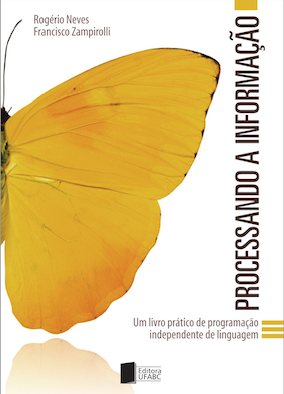
\includegraphics{"figs/Capa_Processando_Informacao.jpg"}

Este caderno (Notebook) é parte complementar \emph{online} do livro
\textbf{\href{https://editora.ufabc.edu.br/matematica-e-ciencias-da-computacao/58-processando-a-informacao}{Processando
a Informação}: um livro prático de programação independente de
linguagem}, que deve ser consultado no caso de dúvidas sobre os temas
apresentados.

\begin{quote}
Este conteúdo pode ser copiado e alterado livremente e foi inspirado
nesse livro.
\end{quote}

    \hypertarget{exercuxedcios}{%
\subsubsection{Exercícios}\label{exercuxedcios}}

{[}Fonte:
\href{https://www.studocu.com/pt-br/document/universidade-estadual-da-paraiba/algoritmos/tarefas-obrigatorias/lista-de-exercicio-respondido-em-python-estrutura-condicional/4958982/view}{link}{]}

    \begin{center}\rule{0.5\linewidth}{0.5pt}\end{center}

\begin{enumerate}
\def\labelenumi{\arabic{enumi}.}
\tightlist
\item
  Fazer um programa que leia a capacidade de um elevador e o peso de 5
  pessoas. Informar se o elevador está liberado para subir ou se excedeu
  a carga máxima.
\end{enumerate}

    \begin{center}\rule{0.5\linewidth}{0.5pt}\end{center}

\begin{enumerate}
\def\labelenumi{\arabic{enumi}.}
\setcounter{enumi}{1}
\tightlist
\item
  Faça um programa que leia 4 variáveis A, B, C e D. A seguir, se B for
  maior do que C e se D for maior do que A e a soma de C com D for maior
  que a soma de A e B e se C e D, ambos, forem positivos e se a variável
  A for par, escrever a mensagem ``valores aceitos'', senão escrever
  ``valores não aceitos''
\end{enumerate}

    \begin{center}\rule{0.5\linewidth}{0.5pt}\end{center}

\begin{enumerate}
\def\labelenumi{\arabic{enumi}.}
\setcounter{enumi}{2}
\tightlist
\item
  Escreva um programa que informe se um dado ano é ou não é bissexto. Um
  ano é bissexto se ele for divisível por 400 ou se ele for divisível
  por 4 e não por 100.
\end{enumerate}

    \begin{center}\rule{0.5\linewidth}{0.5pt}\end{center}

\begin{enumerate}
\def\labelenumi{\arabic{enumi}.}
\setcounter{enumi}{3}
\tightlist
\item
  Construa um programa que leia um número inteiro e imprima a quantidade
  de centenas, dezenas e unidades desse número. Considere o seguinte
  exemplo: o número 345 possui 3 centenas, 4 dezenas e 5 unidades.
\end{enumerate}

    \begin{center}\rule{0.5\linewidth}{0.5pt}\end{center}

\begin{enumerate}
\def\labelenumi{\arabic{enumi}.}
\setcounter{enumi}{4}
\tightlist
\item
  Faça um programa que pergunte o nome do aluno, a quantidade de dias na
  semana e o tipo de curso (B para básico, I para intermediário e A para
  avançado). Mostre o nome do aluno e o valor a ser pago. O valor total
  é calculado com base nas informações abaixo:
\end{enumerate}

\begin{itemize}
\tightlist
\item
  Caso a opção escolhida for Básico, deverá fazer a seguinte conta:
  \textgreater{} Valor Total = (Quantidade de dias na semana * 7 ) * 15
\item
  Caso a opção escolhida for Intermediário, deverá fazer a seguinte
  conta: \textgreater{} Valor Total = (Quantidade de dias na semana *
  8,5 ) * 20
\item
  Caso a opção escolhida for Avançado, deverá fazer a seguinte conta:
  \textgreater{} Valor Total = (Quantidade de dias na semana * 10 ) * 25
\end{itemize}

    \hypertarget{processando-a-informauxe7uxe3o-cap.-3-desvios-condicionais---pruxe1tica-3}{%
\subsection{Processando a Informação: Cap. 3: Desvios Condicionais -
Prática
3}\label{processando-a-informauxe7uxe3o-cap.-3-desvios-condicionais---pruxe1tica-3}}

    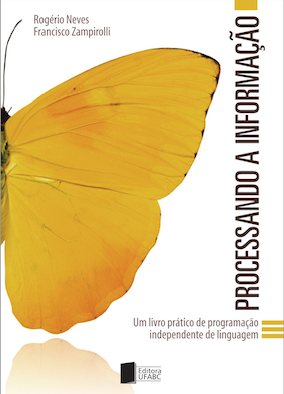
\includegraphics{"figs/Capa_Processando_Informacao.jpg"}

Este caderno (Notebook) é parte complementar \emph{online} do livro
\textbf{\href{https://editora.ufabc.edu.br/matematica-e-ciencias-da-computacao/58-processando-a-informacao}{Processando
a Informação}: um livro prático de programação independente de
linguagem}, que deve ser consultado no caso de dúvidas sobre os temas
apresentados.

\begin{quote}
Este conteúdo pode ser copiado e alterado livremente e foi inspirado
nesse livro.
\end{quote}

    \hypertarget{exercuxedcios}{%
\subsubsection{Exercícios}\label{exercuxedcios}}

{[}Fonte:
\href{http://www.facom.ufu.br/~backes/gbt017/ListaPython02.pdf}{link}{]}

    \begin{center}\rule{0.5\linewidth}{0.5pt}\end{center}

\begin{enumerate}
\def\labelenumi{\arabic{enumi}.}
\tightlist
\item
  Faça um programa que leia 2 notas de um aluno, verifique se as notas
  sao válidas e exiba na tela a média destas notas. Uma nota válida deve
  ser, obrigatoriamente, um valor entre 0.0 e 10.0, onde caso a nota não
  possua um valor válido, este fato deve ser informado ao usuário e o
  programa termina.
\end{enumerate}

    \begin{center}\rule{0.5\linewidth}{0.5pt}\end{center}

\begin{enumerate}
\def\labelenumi{\arabic{enumi}.}
\setcounter{enumi}{1}
\tightlist
\item
  Escreva um programa que leia um número inteiro maior do que zero e
  devolva, na tela, a soma de todos os seus algarismos. Por exemplo, ao
  numero 251 corresponder ao valor 8 (2 + 5 + 1). Se o numero lido não
  for maior do que zero, o programa terminará com a mensagem ``Numero
  inválido''.
\end{enumerate}

    \begin{center}\rule{0.5\linewidth}{0.5pt}\end{center}

\begin{enumerate}
\def\labelenumi{\arabic{enumi}.}
\setcounter{enumi}{2}
\tightlist
\item
  Escreva um programa que leia um inteiro entre 1 e 12 e imprima o mês
  correspondente a este número. Isto é, janeiro se 1, fevereiro se 2, e
  assim por diante.
\end{enumerate}

    \begin{center}\rule{0.5\linewidth}{0.5pt}\end{center}

\begin{enumerate}
\def\labelenumi{\arabic{enumi}.}
\setcounter{enumi}{3}
\tightlist
\item
  Faça uma função que calcule e retorne a área de um trapézio (A).
  Lembre-se que a base maior e a base menor devem ser números maiores
  que zero.
\end{enumerate}

\[ A = \frac{altura*(basemaior + basemenor)}{2}\]

    \begin{center}\rule{0.5\linewidth}{0.5pt}\end{center}

\begin{enumerate}
\def\labelenumi{\arabic{enumi}.}
\setcounter{enumi}{4}
\tightlist
\item
  Faça um programa para verificar se um determinado número inteiro e
  divisível por 3 ou 5, mas nao simultaneamente pelos dois.
\end{enumerate}

    \begin{center}\rule{0.5\linewidth}{0.5pt}\end{center}

\begin{enumerate}
\def\labelenumi{\arabic{enumi}.}
\setcounter{enumi}{5}
\tightlist
\item
  Escreva o menu de opções abaixo. Leia a opção do usuário e execute a
  operação escolhida. Escreva uma mensagem de erro se a opção for
  inválida.
\end{enumerate}

\begin{verbatim}
Escolha a opção:
1- Soma de 2 números.
2- Diferença entre 2 números (maior pelo menor).
3- Produto entre 2 números.
4- Divisão entre 2 números (o denominador não pode ser zero).
Opção
\end{verbatim}

    \begin{center}\rule{0.5\linewidth}{0.5pt}\end{center}

\begin{enumerate}
\def\labelenumi{\arabic{enumi}.}
\setcounter{enumi}{6}
\tightlist
\item
  Leia a idade e o tempo de serviço de um trabalhador e escreva se ele
  pode ou não se aposentar. As condições para aposentadoria são:
\end{enumerate}

\begin{itemize}
\tightlist
\item
  Ter pelo menos 65 anos,
\item
  Ou ter trabalhado pelo menos 30 anos,
\item
  Ou ter pelo menos 60 anos e trabalhado pelo menos 25 anos.
\end{itemize}

    \begin{center}\rule{0.5\linewidth}{0.5pt}\end{center}

\begin{enumerate}
\def\labelenumi{\arabic{enumi}.}
\setcounter{enumi}{7}
\tightlist
\item
  Uma empresa vende o mesmo produto para quatro diferentes estados. Cada
  estado possui uma taxa diferente de imposto sobre o produto (MG 7\%;
  SP 12\%; RJ 15\%; MS 8\%). Faça um programa em que o usuario entre com
  o valor e o estado destino do produto e o programa retorne o preço
  final do produto acrescido do imposto do estado em que ele será
  vendido. Se o estado digitado não for válido, mostrar uma mensagem de
  erro.
\end{enumerate}

    \begin{center}\rule{0.5\linewidth}{0.5pt}\end{center}

\begin{enumerate}
\def\labelenumi{\arabic{enumi}.}
\setcounter{enumi}{8}
\tightlist
\item
  Leia a distância em Km e a quantidade de litros de gasolina consumidos
  por um carro em um percurso, calcule o consumo em Km/l e escreva uma
  mensagem de acordo com a tabela abaixo:
\end{enumerate}

\begin{longtable}[]{@{}lll@{}}
\toprule
Consumo & Km/l & Mensagem\tabularnewline
\midrule
\endhead
menor que & 8 & venda o carro!\tabularnewline
entre & 8 e 14 & econômico!\tabularnewline
maior que & 14 & super econômico!\tabularnewline
\bottomrule
\end{longtable}

    \begin{center}\rule{0.5\linewidth}{0.5pt}\end{center}

\begin{enumerate}
\def\labelenumi{\arabic{enumi}.}
\setcounter{enumi}{9}
\tightlist
\item
  Escreva um programa que, dada a idade de um nadador, classifique-o em
  uma das seguintes categorias:
\end{enumerate}

\begin{longtable}[]{@{}ll@{}}
\toprule
Categora & Idade\tabularnewline
\midrule
\endhead
Infantil A & 5 a 7\tabularnewline
Infantil B & 8 a 10\tabularnewline
Juvenil A & 11 a 13\tabularnewline
Juvenil B & 14 a 17\tabularnewline
Sênior & maior que 17\tabularnewline
\bottomrule
\end{longtable}

    \begin{center}\rule{0.5\linewidth}{0.5pt}\end{center}

\begin{enumerate}
\def\labelenumi{\arabic{enumi}.}
\setcounter{enumi}{10}
\tightlist
\item
  Escrever um programa que leia o codigo do produto escolhido do
  cardápio de uma lanchonete e a quantidade. O programa deve calcular o
  valor a será pago por aquele lanche. Considere que a cada execução
  somente será calculado um pedido. O cardápio da lanchonete segue o
  padrao abaixo:
\end{enumerate}

\begin{longtable}[]{@{}lll@{}}
\toprule
Especificação & Código & Preço\tabularnewline
\midrule
\endhead
Cachorro quente & 100 & 12.0\tabularnewline
Bauru Simples & 101 & 13.0\tabularnewline
Bauru Simples & 102 & 13.0\tabularnewline
Hamburguer & 103 & 12.0\tabularnewline
Cheeseburguer & 104 & 17.0\tabularnewline
Suco & 105 & 6.0\tabularnewline
Refrigerante & 106 & 4.0\tabularnewline
\bottomrule
\end{longtable}

    \hypertarget{processando-a-informauxe7uxe3o-cap.-4-estruturas-de-repetiuxe7uxe3o-lauxe7os}{%
\section{Processando a Informação: Cap. 4: Estruturas de Repetição
(Laços)}\label{processando-a-informauxe7uxe3o-cap.-4-estruturas-de-repetiuxe7uxe3o-lauxe7os}}

    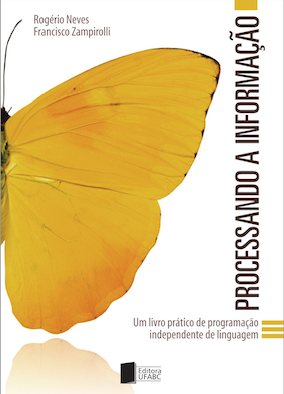
\includegraphics{"figs/Capa_Processando_Informacao.jpg"}

Este caderno (Notebook) é parte complementar \emph{online} do livro
\textbf{\href{https://editora.ufabc.edu.br/matematica-e-ciencias-da-computacao/58-processando-a-informacao}{Processando
a Informação}: um livro prático de programação independente de
linguagem}, que deve ser consultado no caso de dúvidas sobre os temas
apresentados.

\begin{quote}
Este conteúdo pode ser copiado e alterado livremente e foi inspirado
nesse livro.
\end{quote}

    \hypertarget{sumuxe1rio}{%
\subsection{Sumário}\label{sumuxe1rio}}

\begin{itemize}
\tightlist
\item
  Revisão do capítulo anterios
\item
  Quando usar repetições?
\item
  Tipos de estruturas de repetição
\item
  Laços aninhados
\item
  Validação de dados com laços
\item
  Interrupção da execução dos laços
\item
  Recursão
\item
  Revisão deste capítulo
\item
  Exercícios
\end{itemize}

    \hypertarget{revisuxe3o-do-capuxedtulo-anterior-desvios-condicionais}{%
\subsection{Revisão do capítulo anterior (Desvios
Condicionais)}\label{revisuxe3o-do-capuxedtulo-anterior-desvios-condicionais}}

    \begin{itemize}
\item
  No capítulo anterior foram apresentadas formas de construir código
  contendo estruturas condicionais simples ou compostas. Ou seja,
  desvios condicionais, da forma:

  \begin{itemize}
  \tightlist
  \item
    \texttt{se} algo for verdade, \texttt{então}

    \begin{itemize}
    \tightlist
    \item
      faça algo1,
    \end{itemize}
  \item
    \texttt{senão} \# essa parte é opcional

    \begin{itemize}
    \tightlist
    \item
      faça algo2.
    \end{itemize}
  \end{itemize}
\item
  Neste capítulo iremos abordar as \textbf{Estruturas de Repetição},
  conhecidas também como \textbf{Laços} ou \textbf{\emph{Loops}}.
\end{itemize}

    \hypertarget{quando-usar-repetiuxe7uxf5es}{%
\subsection{Quando usar
repetições?}\label{quando-usar-repetiuxe7uxf5es}}

    \begin{itemize}
\item
  As estruturas de repetição são recomendadas para quando um padrão de
  código é repetido várias vezes sequencialmente, apenas alterando-se o
  valor de uma ou mais variáveis entre os comandos repetidos.
\item
  Veja no exemplo a seguir um pseudocodigo, para imprimir a tabuada de
  um número \texttt{t} entrado pelo usuário no formato:
\end{itemize}

Tabuada x (número de 1 a 10) = valor

    \begin{verbatim}
Inteiro: t, n = 1;
t = leia("Qual a tabuada? "); 
escreva(t + " x " + n + " = " + t * n);        n = n + 1; 
escreva(t + " x " + n + " = " + t * n);        n = n + 1; 
escreva(t + " x " + n + " = " + t * n);        n = n + 1; 
escreva(t + " x " + n + " = " + t * n);        n = n + 1; 
escreva(t + " x " + n + " = " + t * n);        n = n + 1; 
escreva(t + " x " + n + " = " + t * n);        n = n + 1; 
escreva(t + " x " + n + " = " + t * n);        n = n + 1; 
escreva(t + " x " + n + " = " + t * n);        n = n + 1; 
escreva(t + " x " + n + " = " + t * n);        n = n + 1; 
escreva(t + " x " + n + " = " + t * n);        n = n + 1; 
\end{verbatim}

    \begin{itemize}
\tightlist
\item
  Embora o código não pareça extenso, é fácil imaginar uma situação onde
  tenhamos que repetir 100, 500, 1000 vezes um mesmo bloco de
  instruções.
\end{itemize}

    \hypertarget{tipos-de-estruturas-de-repetiuxe7uxe3o}{%
\subsection{Tipos de estruturas de
repetição}\label{tipos-de-estruturas-de-repetiuxe7uxe3o}}

    \hypertarget{pseudocuxf3digo}{%
\subsubsection{Pseudocódigo}\label{pseudocuxf3digo}}

    \hypertarget{fauxe7a-enquanto}{%
\paragraph{faça-enquanto}\label{fauxe7a-enquanto}}

\begin{verbatim}
faça { 
  comandos 
} enquanto (condição);
\end{verbatim}

    \hypertarget{enquanto-fauxe7a}{%
\paragraph{enquanto-faça}\label{enquanto-fauxe7a}}

\begin{verbatim}
enquanto (condição) faça { 
  comandos 
}
\end{verbatim}

    \hypertarget{para}{%
\paragraph{para}\label{para}}

\begin{verbatim}
para variável = valor_inicial até valor_final, variável++, faça { 
  comandos 
}
\end{verbatim}

    \hypertarget{para-reverso}{%
\paragraph{para reverso}\label{para-reverso}}

\begin{verbatim}
para variável = valor_final até valor_inicial, variável--, faça { 
  comandos 
}
\end{verbatim}

    \begin{itemize}
\item
  Note que no caso do \texttt{enquanto-faça} é necessário que a condição
  seja verdadeira para que os comandos presentes no bloco de execução
  sejam processados.
\item
  Neste caso, se ao entrar no comando enquanto (\emph{while}) a condição
  do teste for falsa, oposto ao \texttt{faça-enquanto}, o subprograma
  não será executado.
\item
  Isto é, todo o código dentro do bloco do laço será pulado já na
  verificação inicial da condição no \texttt{enquanto-faça}, seguindo
  diretamente para a parte sequencial subsequente, similar ao que ocorre
  no se-então.
\item
  A forma \texttt{faça-enquanto} é recomendada quando queremos que os
  comandos contidos no laço sejam executados ao menos uma vez, mesmo que
  a condição seja inicialmente falsa.
\item
  O laço \texttt{para} é recomendado quando se sabe o número de
  iterações existes (quantas vezes o bloco dentro do laço será
  executado). Por exempo, no caso anterior do problema da Tabuada.
\end{itemize}

    \hypertarget{ccppjavajavascript}{%
\subsubsection{C/CPP/Java/JavaScript}\label{ccppjavajavascript}}

    \hypertarget{do-while}{%
\paragraph{do-while}\label{do-while}}

    \begin{verbatim}
do { 
  comandos;
} while (condição);
\end{verbatim}

    \hypertarget{while}{%
\paragraph{while}\label{while}}

    \begin{verbatim}
while (condição) { 
  comandos;
}
\end{verbatim}

    \hypertarget{for}{%
\paragraph{for}\label{for}}

    \begin{verbatim}
for(v=0; v<10; v++) {
  comandos;
}
\end{verbatim}

Em algumas linguagens de programação é possível omitir um ou todos os
parâmetros, por exemplo: \texttt{for(;;)\ \{...\}}.

    \hypertarget{pseudocuxf3digo-exemplo-lauxe7o-fauxe7a-enquanto.}{%
\subsubsection{Pseudocódigo: Exemplo laço
faça-enquanto.}\label{pseudocuxf3digo-exemplo-lauxe7o-fauxe7a-enquanto.}}

\begin{verbatim}
Real: nota, média, acumulador=0, contador=0;
Caractere: resposta='lixo';

faça {
   nota = leia("Entre com uma nota: ");
   acumulador = acumulador + nota;
   contador = contador + 1;
   resposta = leia("Deseja continuar? (s/n): ");
} enquanto (resposta == 's');

média = acumulador / contador;
imprima ("A média das " + contador + " notas é " + média);
\end{verbatim}

    \begin{itemize}
\item
  Além do \texttt{contador}, o programa usa um \texttt{acumulador}
  (variável que acumula as notas digitadas).
\item
  Repare que a condição
  \texttt{resposta\ ==\ \textquotesingle{}s\textquotesingle{}} no
  \texttt{faça-enquanto} é falsa até que seja efetuada a leitura da
  variável resposta dentro do laço, em:
  \texttt{resposta\ =\ leia("Deseja\ continuar?\ (s/n):\ ");}
\item
  Apenas do caso de o usuário entrar com o caractere
  \texttt{\textquotesingle{}s\textquotesingle{}}, o laço será repetido
  novamente.
\item
  Isto quer dizer que o estado da condição é falso na primeira execução
  do código do laço.
\end{itemize}

    \hypertarget{pseudocuxf3digo-exemplo-lauxe7o-enquanto-fauxe7a.}{%
\subsubsection{Pseudocódigo: Exemplo laço
enquanto-faça.}\label{pseudocuxf3digo-exemplo-lauxe7o-enquanto-fauxe7a.}}

\begin{verbatim}
Real: nota, média, acumulador=0, contador=0;
Caractere: resposta='s';

enquanto (resposta == 's') faça {
   nota = leia("Entre com uma nota: ");
   acumulador = acumulador + nota;
   contador = contador + 1;
   resposta = leia("Deseja continuar? (s/n): ");
} 

média = acumulador / contador;
imprima ("A média das " + contador + " notas é " + média);
\end{verbatim}

    \begin{itemize}
\tightlist
\item
  Observe que no pseudocódigo anterior do \texttt{enquanto-faça} temos o
  mesmo resultado do \texttt{faça-enquanto}, pois a variável
  \texttt{resposta} é inicializada com \texttt{s}, satisfazendo a
  condição lógica e entrando no laço.
\end{itemize}

    \begin{itemize}
\tightlist
\item
  Ver Fluxograma abaixo (também experimente nessa ferramenta
  \emph{online}: \href{https://app.code2flow.com/}{code2flow}, copiando
  e colando o código em vermelho abaixo):
\end{itemize}

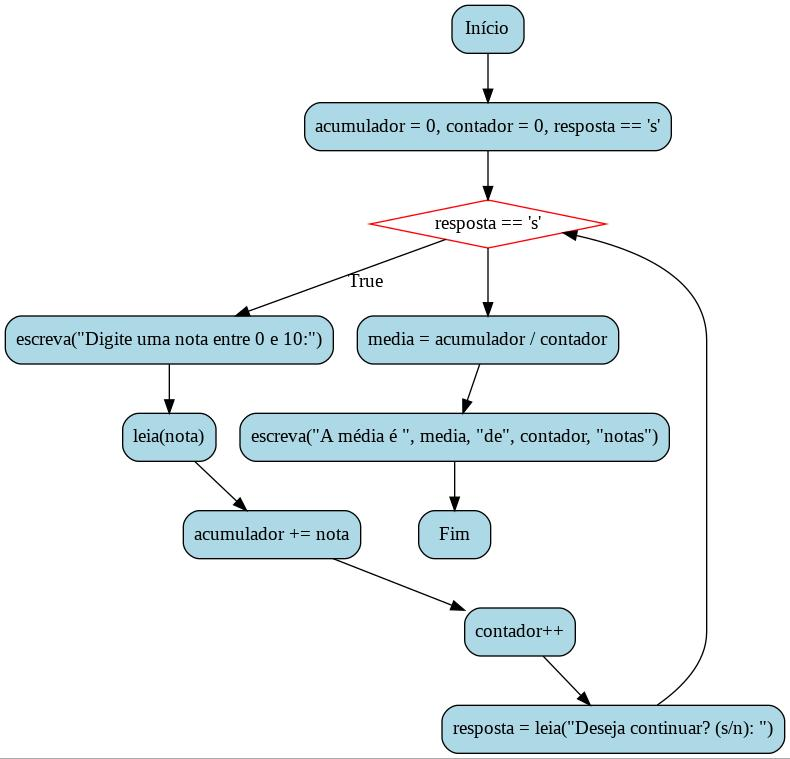
\includegraphics{"figs/flowchartCap4a.png"}

    \begin{figure}
\centering
\caption{flowchartCap4a.png}
\end{figure}

    \begin{tcolorbox}[breakable, size=fbox, boxrule=1pt, pad at break*=1mm,colback=cellbackground, colframe=cellborder]
\prompt{In}{incolor}{ }{\boxspacing}
\begin{Verbatim}[commandchars=\\\{\}]
\PY{o}{!}apt\PYZhy{}get install graphviz libgraphviz\PYZhy{}dev pkg\PYZhy{}config
\PY{o}{!}pip install txtoflow
\end{Verbatim}
\end{tcolorbox}

    \begin{tcolorbox}[breakable, size=fbox, boxrule=1pt, pad at break*=1mm,colback=cellbackground, colframe=cellborder]
\prompt{In}{incolor}{ }{\boxspacing}
\begin{Verbatim}[commandchars=\\\{\}]
\PY{k+kn}{from} \PY{n+nn}{txtoflow} \PY{k+kn}{import} \PY{n}{txtoflow}

\PY{n}{txtoflow}\PY{o}{.}\PY{n}{generate}\PY{p}{(}
    \PY{l+s+sd}{\PYZsq{}\PYZsq{}\PYZsq{}}
\PY{l+s+sd}{    Início;}
\PY{l+s+sd}{    acumulador = 0, contador = 0, resposta == \PYZsq{}s\PYZsq{};}
\PY{l+s+sd}{    while (resposta == \PYZsq{}s\PYZsq{}) \PYZob{}}
\PY{l+s+sd}{      escreva(\PYZdq{}Digite uma nota entre 0 e 10:\PYZdq{});}
\PY{l+s+sd}{      leia(nota);}
\PY{l+s+sd}{      acumulador += nota;}
\PY{l+s+sd}{      contador++;}
\PY{l+s+sd}{      resposta = leia(\PYZdq{}Deseja continuar? (s/n): \PYZdq{});}
\PY{l+s+sd}{    \PYZcb{}}
\PY{l+s+sd}{    media = acumulador / contador;}
\PY{l+s+sd}{    escreva(\PYZdq{}A média é \PYZdq{}, media, \PYZdq{}de\PYZdq{}, contador, \PYZdq{}notas\PYZdq{});}
\PY{l+s+sd}{    Fim;}
\PY{l+s+sd}{    \PYZsq{}\PYZsq{}\PYZsq{}}
\PY{p}{)}
\end{Verbatim}
\end{tcolorbox}

    \hypertarget{pseudocuxf3digo-exemplo-lauxe7o-enquanto-fauxe7a-infinito.}{%
\subsubsection{Pseudocódigo: Exemplo laço enquanto-faça
INFINITO.}\label{pseudocuxf3digo-exemplo-lauxe7o-enquanto-fauxe7a-infinito.}}

Considere uma alteração no código anterior para não fazer mais a
pergunta \texttt{Deseja\ continuar?\ (s/n)}, mas entrando num laço
\texttt{enquanto-faça} para ler e acumular 100 notas:

\begin{verbatim}
Real: nota, média, acumulador=0,contador=0;

enquanto (contador < 100) faça {
   nota = leia("Entre com uma nota: ");
   acumulador = acumulador + nota;
   # contador = contador + 1;
} 

média = acumulador / contador;
imprima ("A média das " + contador + " notas é " + média);
\end{verbatim}

    \begin{itemize}
\tightlist
\item
  O que vai ocorrer ao escrever e rodar esse código em alguma linguagem
  de programação?
\item
  Onde está o erro?
\item
  \textbf{MUITO CUIDADO COM LAÇOS INFINITOS EM ATIVIDADES NO
  MOODLE+VPL!} Se a execução demorar mais que 1 minuto, provavelmente
  entrou em um laço infinito e terá que recarregar a página.
\item
  Esta condição, onde a execução fica ``presa'' dentro do laço, é
  conhecida como \textbf{\emph{DEADLOCK}}.
\item
  \emph{Deadlocks} geram erro de finalização de programa, que executará
  eternamente, podendo travar o programa, o teclado e o mouse ou até
  mesmo o computador, neste caso, sendo necessário um
  \textbf{\emph{RESET}} para sair do laço.
\end{itemize}

    \hypertarget{validauxe7uxe3o-de-dados}{%
\subsection{Validação de Dados}\label{validauxe7uxe3o-de-dados}}

    \begin{itemize}
\item
  Uma possível aplicação de laços é garantir que os dados entrados sejam
  válidos.
\item
  \textbf{Validação de dados} é o nome dado à verificação dos valores de
  entrada, se os mesmos se encontram dentro dos limites previstos ou no
  formato adequado, notificando o usuário no caso de valores inválidos.
\item
  O exemplo a seguir é o pseudocódigo apresentado anteriormente,
  incorporando a validação de dados de entrada (nota entre 0 e 10),
  indicando o erro e pedindo para o usuário entrar novamente o dado até
  que seja válido.
\end{itemize}

    \hypertarget{pseudocuxf3digo-exemplo-lauxe7o-fauxe7a-enquanto-com-validauxe7uxe3o}{%
\subsubsection{Pseudocódigo: Exemplo laço faça-enquanto, com
validação}\label{pseudocuxf3digo-exemplo-lauxe7o-fauxe7a-enquanto-com-validauxe7uxe3o}}

\begin{verbatim}
Real: nota, média, acumulador=0, contador=0;
Caractere: resposta='lixo';

faça {
  faça {
    nota = leia("Entre com uma nota entre 0 e 10: ");
    se (nota < 0 || nota > 10) então 
      escreva("ERRO, nota inválida. Digital nota entre 0 e 10!")
  } enquanto (nota < 0 || nota > 10); 
  acumulador = acumulador + nota;
  contador = contador + 1;
  resposta = leia("Deseja continuar? (s/n): ");
} enquanto (resposta == 's');

média = acumulador / contador;
imprima ("A média das " + contador + " notas é " + média);
\end{verbatim}

    \begin{itemize}
\tightlist
\item
  No pseudocódigo anterior, o segundo \texttt{faça-enquanto} aceita
  apenas notas entre 0 e 10. Caso contrário, escreve uma mensagem de
  erro e solicita nova nota.
\end{itemize}

    \begin{itemize}
\item
  Ver Fluxograma abaixo (também experimente nessa ferramenta
  \emph{online}: \href{https://app.code2flow.com/}{code2flow}, copiando
  e colando o código em vermelho abaixo).
\item
  Observar que essa biblioteca \texttt{txtoflow} não aceita
  \texttt{faça-enquanto}, assim como o Python.
\end{itemize}

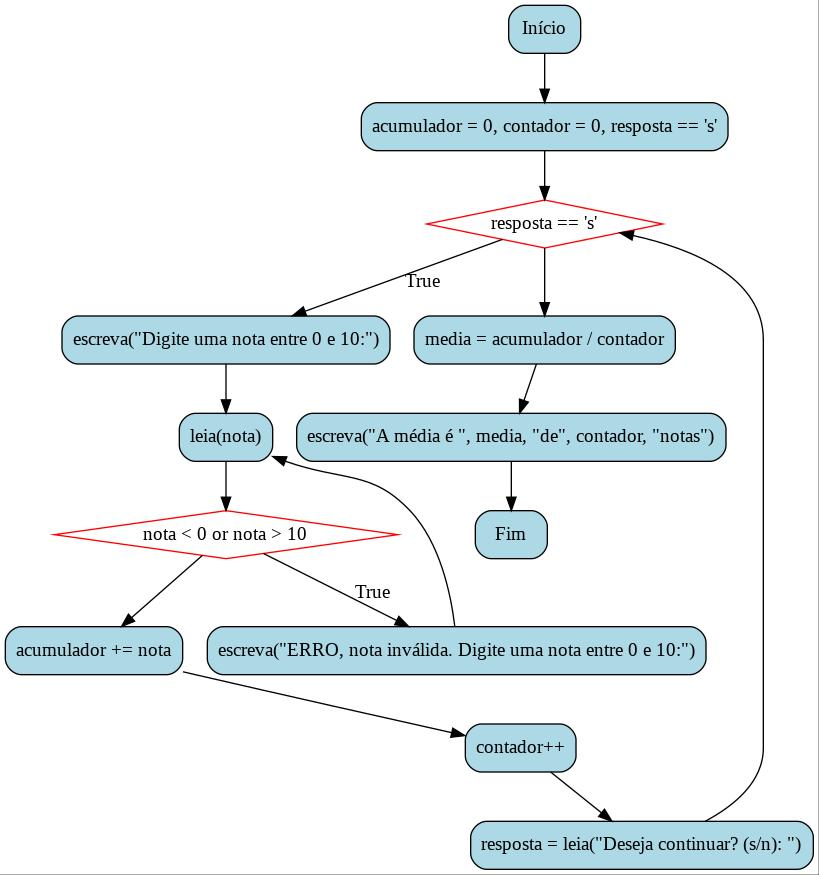
\includegraphics{"figs/flowchartCap4b.png"}

    \begin{figure}
\centering
\caption{flowchartCap4b.png}
\end{figure}

    \begin{tcolorbox}[breakable, size=fbox, boxrule=1pt, pad at break*=1mm,colback=cellbackground, colframe=cellborder]
\prompt{In}{incolor}{ }{\boxspacing}
\begin{Verbatim}[commandchars=\\\{\}]
\PY{o}{!}apt\PYZhy{}get install graphviz libgraphviz\PYZhy{}dev pkg\PYZhy{}config
\PY{o}{!}pip install txtoflow
\end{Verbatim}
\end{tcolorbox}

    \begin{tcolorbox}[breakable, size=fbox, boxrule=1pt, pad at break*=1mm,colback=cellbackground, colframe=cellborder]
\prompt{In}{incolor}{ }{\boxspacing}
\begin{Verbatim}[commandchars=\\\{\}]
\PY{k+kn}{from} \PY{n+nn}{txtoflow} \PY{k+kn}{import} \PY{n}{txtoflow}

\PY{n}{txtoflow}\PY{o}{.}\PY{n}{generate}\PY{p}{(}
    \PY{l+s+sd}{\PYZsq{}\PYZsq{}\PYZsq{}}
\PY{l+s+sd}{    Início;}
\PY{l+s+sd}{    acumulador = 0, contador = 0, resposta == \PYZsq{}s\PYZsq{};}
\PY{l+s+sd}{    while (resposta == \PYZsq{}s\PYZsq{}) \PYZob{}}
\PY{l+s+sd}{      escreva(\PYZdq{}Digite uma nota entre 0 e 10:\PYZdq{});}
\PY{l+s+sd}{      leia(nota);}
\PY{l+s+sd}{      while (nota \PYZlt{} 0 or nota \PYZgt{} 10) \PYZob{}}
\PY{l+s+sd}{        escreva(\PYZdq{}ERRO, nota inválida. Digite uma nota entre 0 e 10:\PYZdq{});}
\PY{l+s+sd}{        leia(nota);}
\PY{l+s+sd}{      \PYZcb{}}
\PY{l+s+sd}{      acumulador += nota;}
\PY{l+s+sd}{      contador++;}
\PY{l+s+sd}{      resposta = leia(\PYZdq{}Deseja continuar? (s/n): \PYZdq{});}
\PY{l+s+sd}{    \PYZcb{}}
\PY{l+s+sd}{    media = acumulador / contador;}
\PY{l+s+sd}{    escreva(\PYZdq{}A média é \PYZdq{}, media, \PYZdq{}de\PYZdq{}, contador, \PYZdq{}notas\PYZdq{});}
\PY{l+s+sd}{    Fim;}
\PY{l+s+sd}{    \PYZsq{}\PYZsq{}\PYZsq{}}
\PY{p}{)}
\end{Verbatim}
\end{tcolorbox}

    \hypertarget{interrupuxe7uxe3o-dos-lauxe7os}{%
\subsection{Interrupção dos
laços}\label{interrupuxe7uxe3o-dos-lauxe7os}}

    \begin{itemize}
\item
  Algumas linguagens permitem interromper a execução do laço através do
  comando `interromper' ou `quebrar' (\textbf{break}).
\item
  Isto pode ser útil caso se queira interromper o laço em algum evento
  específico.
\end{itemize}

    \hypertarget{exemplo-01---ler-10-notas-com-validauxe7uxe3o}{%
\subsection{Exemplo 01 - Ler 10 notas com
validação}\label{exemplo-01---ler-10-notas-com-validauxe7uxe3o}}

Considere um algoritmo para ler 10 notas válidas, entre 0 e 10,
escrevendo no final a média nas notas válidas lidas.

    Pseudocódigo

\begin{verbatim}
Real: nota, média, acumulador=0,contador=0;

escreva("Entre com 10 notas válidas")
faça {
  faça {
    nota = leia();
  } enquanto (nota < 0 || nota > 10); 
  acumulador = acumulador + nota;
  contador = contador + 1;
} enquanto (contador < 10);

média = acumulador / contador;
escreva("A média das " + contador + " notas é " + média);
\end{verbatim}

    \begin{itemize}
\tightlist
\item
  Ver Fluxograma abaixo (também experimente nessa ferramenta
  \emph{online}: \href{https://app.code2flow.com/}{code2flow}, copiando
  e colando o código em vermelho abaixo):
\end{itemize}

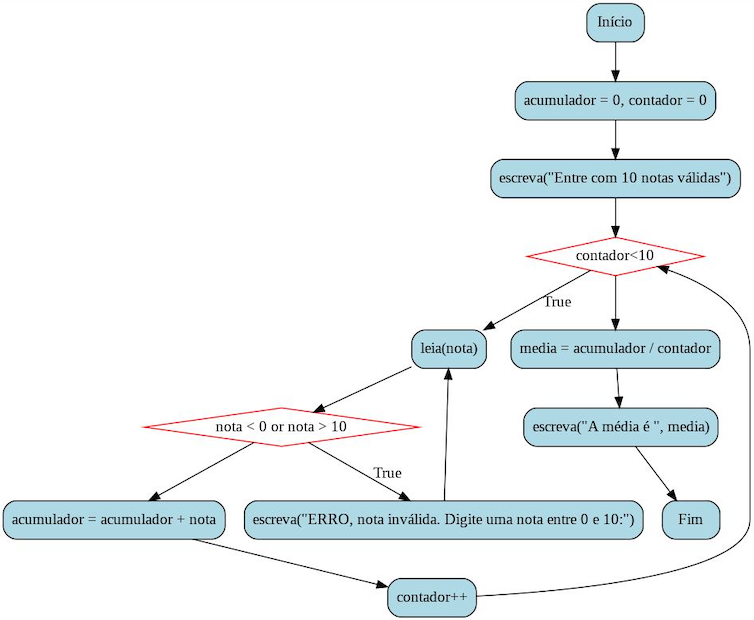
\includegraphics{"figs/flowchartCap4c.png"}

    \begin{figure}
\centering
\caption{flowchartCap4c.jpg}
\end{figure}

    \begin{tcolorbox}[breakable, size=fbox, boxrule=1pt, pad at break*=1mm,colback=cellbackground, colframe=cellborder]
\prompt{In}{incolor}{ }{\boxspacing}
\begin{Verbatim}[commandchars=\\\{\}]
\PY{o}{!}apt\PYZhy{}get install graphviz libgraphviz\PYZhy{}dev pkg\PYZhy{}config
\PY{o}{!}pip install txtoflow
\end{Verbatim}
\end{tcolorbox}

    \begin{tcolorbox}[breakable, size=fbox, boxrule=1pt, pad at break*=1mm,colback=cellbackground, colframe=cellborder]
\prompt{In}{incolor}{ }{\boxspacing}
\begin{Verbatim}[commandchars=\\\{\}]
\PY{k+kn}{from} \PY{n+nn}{txtoflow} \PY{k+kn}{import} \PY{n}{txtoflow}

\PY{n}{txtoflow}\PY{o}{.}\PY{n}{generate}\PY{p}{(}
    \PY{l+s+sd}{\PYZsq{}\PYZsq{}\PYZsq{}}
\PY{l+s+sd}{    Início;}
\PY{l+s+sd}{    acumulador = 0, contador = 0;}
\PY{l+s+sd}{    escreva(\PYZdq{}Entre com 10 notas válidas\PYZdq{});}
\PY{l+s+sd}{    while (contador\PYZlt{}10) \PYZob{}}
\PY{l+s+sd}{      leia(nota);}
\PY{l+s+sd}{      while (nota \PYZlt{} 0 or nota \PYZgt{} 10) \PYZob{}}
\PY{l+s+sd}{        escreva(\PYZdq{}ERRO, nota inválida. Digite uma nota entre 0 e 10:\PYZdq{});}
\PY{l+s+sd}{        leia(nota);}
\PY{l+s+sd}{      \PYZcb{}}
\PY{l+s+sd}{      acumulador = acumulador + nota;}
\PY{l+s+sd}{      contador++;}
\PY{l+s+sd}{    \PYZcb{}}
\PY{l+s+sd}{    media = acumulador / contador;}
\PY{l+s+sd}{    escreva(\PYZdq{}A média é \PYZdq{}, media);}
\PY{l+s+sd}{    Fim;}
\PY{l+s+sd}{    \PYZsq{}\PYZsq{}\PYZsq{}}
\PY{p}{)}
\end{Verbatim}
\end{tcolorbox}

    Casos para Teste Moodle+VPL

Para o professor criar uma atividade VPL no Moodle para este Exemplo 01,
basta incluir em \texttt{Casos\ para\ teste}, o seguinte texto (pode
incluir mais casos):

\begin{verbatim}
case=caso1
input=9.0
78.0
6.0
9
8
7
6
5
7
8
6
output= 
A média das 10 notas é 7.1
case=caso2
input=9.0
78.0
-9.0
9876.0
9876.0
7.0
9
8
4
6
6
8
9
7
output= 
A média das 10 notas é 7.3
\end{verbatim}

    \begin{tcolorbox}[breakable, size=fbox, boxrule=1pt, pad at break*=1mm,colback=cellbackground, colframe=cellborder]
\prompt{In}{incolor}{1}{\boxspacing}
\begin{Verbatim}[commandchars=\\\{\}]
\PY{o}{\PYZpc{}\PYZpc{}writefile} cap4ex01.c
\PY{c+c1}{\PYZsh{}include \PYZlt{}stdio.h\PYZgt{}}

\PY{n+nb}{int} \PY{n}{main}\PY{p}{(}\PY{n}{void}\PY{p}{)} \PY{p}{\PYZob{}}

  \PY{o}{/}\PY{o}{/} \PY{n}{ENTRADA} \PY{n}{DE} \PY{n}{DADOS} \PY{n}{e} \PY{n}{PROCESSAMENTO}
  \PY{n+nb}{float} \PY{n}{acumulador} \PY{o}{=} \PY{l+m+mi}{0}\PY{p}{,} \PY{n}{nota}\PY{p}{,} \PY{n}{media}\PY{p}{;}
  \PY{n+nb}{int} \PY{n}{contador} \PY{o}{=} \PY{l+m+mi}{0}\PY{p}{;}
  
  \PY{n}{printf}\PY{p}{(}\PY{l+s+s2}{\PYZdq{}}\PY{l+s+s2}{Entre com 10 notas válidas}\PY{l+s+se}{\PYZbs{}n}\PY{l+s+s2}{\PYZdq{}}\PY{p}{)}\PY{p}{;}
  \PY{k}{while} \PY{p}{(}\PY{n}{contador}\PY{o}{\PYZlt{}}\PY{l+m+mi}{10}\PY{p}{)} \PY{p}{\PYZob{}}
    \PY{n}{do} \PY{p}{\PYZob{}}
        \PY{n}{scanf}\PY{p}{(}\PY{l+s+s2}{\PYZdq{}}\PY{l+s+si}{\PYZpc{}f}\PY{l+s+s2}{\PYZdq{}}\PY{p}{,} \PY{o}{\PYZam{}}\PY{n}{nota}\PY{p}{)}\PY{p}{;}
    \PY{p}{\PYZcb{}} \PY{k}{while} \PY{p}{(}\PY{n}{nota} \PY{o}{\PYZlt{}} \PY{l+m+mf}{0.0} \PY{o}{|}\PY{o}{|} \PY{n}{nota} \PY{o}{\PYZgt{}} \PY{l+m+mf}{10.0} \PY{p}{)}\PY{p}{;}
    \PY{n}{acumulador} \PY{o}{=} \PY{n}{acumulador} \PY{o}{+} \PY{n}{nota}\PY{p}{;}
    \PY{n}{contador}\PY{o}{+}\PY{o}{+}\PY{p}{;}
  \PY{p}{\PYZcb{}}
  \PY{n}{media} \PY{o}{=} \PY{n}{acumulador}\PY{o}{/}\PY{n}{contador}\PY{p}{;}

  \PY{o}{/}\PY{o}{/} \PY{n}{SAÍDA}
  \PY{n}{printf}\PY{p}{(}\PY{l+s+s2}{\PYZdq{}}\PY{l+s+s2}{A média das }\PY{l+s+si}{\PYZpc{}d}\PY{l+s+s2}{ notas é }\PY{l+s+si}{\PYZpc{}.1f}\PY{l+s+se}{\PYZbs{}n}\PY{l+s+s2}{\PYZdq{}}\PY{p}{,} \PY{n}{contador}\PY{p}{,} \PY{n}{media}\PY{p}{)}\PY{p}{;}

  \PY{k}{return} \PY{l+m+mi}{0}\PY{p}{;}
\PY{p}{\PYZcb{}}
\end{Verbatim}
\end{tcolorbox}

    \begin{tcolorbox}[breakable, size=fbox, boxrule=1pt, pad at break*=1mm,colback=cellbackground, colframe=cellborder]
\prompt{In}{incolor}{2}{\boxspacing}
\begin{Verbatim}[commandchars=\\\{\}]
\PY{o}{\PYZpc{}\PYZpc{}}\PY{k}{shell}
gcc \PYZhy{}Wall \PYZhy{}std=c99 cap4ex01.c \PYZhy{}o output2
./output2
\end{Verbatim}
\end{tcolorbox}

    \hypertarget{recursuxe3o}{%
\subsection{Recursão}\label{recursuxe3o}}

    Este tópico de recursão (ou recursividade) é complementar ao livro, eu
sua primeira edição.

Como nos laços de repetição, a recursão tem como objetivo rodar trechos
de códigos (agora encapsulados em métodos) várias vezes.

Além disso, análogo ao laço, \textbf{muito cuidado com o critério de
parada, senão o código irá fazer infinitas chamadas recursivas, podendo
travar o seu computador!}

Ou seja, o método recursivo teve ter pelo menos uma condicional e
argumentos que variam nas chamadas recursivas. Veja um exemplo a seguir.

    \hypertarget{exemplo-02---ler-10-notas-com-recursuxe3o}{%
\subsection{Exemplo 02 - Ler 10 notas, com
recursão}\label{exemplo-02---ler-10-notas-com-recursuxe3o}}

Considere um algoritmo para ler 10 notas válidas utilizando recursão e
calcular a média.

    Pseudocódigo

\begin{verbatim}
# MINHA FUNÇÃO RECURSIVA
função lerNota(recebe: real acumulador, inteiro n) retorna real acumulador {
  Real: nota;
  se (n > 0) faça { # CRITÉRIO DE PARADA
    faça {
      nota = leia();
    } enquanto (nota < 0 || nota > 10); 
    acumulador = lerNota(acumulador, n - 1); # CHAMADA RECURSIVA, 
    # COM ALTERAÇÃO DO VALOR DO ARGUMENTO !!!
  }
  retorne acumulador + nota;
}

Real: média, acumulador=0, contador=10;

escreva("Entre com " + contador + " notas válidas")
acumulador = lerNota(acumulador, contador); # CHAMDADA RECURSIVA!!!

média = acumulador / contador;
escreva("A média das " + contador + " notas é " + média);
\end{verbatim}

    \begin{tcolorbox}[breakable, size=fbox, boxrule=1pt, pad at break*=1mm,colback=cellbackground, colframe=cellborder]
\prompt{In}{incolor}{5}{\boxspacing}
\begin{Verbatim}[commandchars=\\\{\}]
\PY{o}{\PYZpc{}\PYZpc{}writefile} cap4ex02.c
\PY{c+c1}{\PYZsh{}include \PYZlt{}stdio.h\PYZgt{}}

\PY{n+nb}{float} \PY{n}{lerNota}\PY{p}{(}\PY{n+nb}{float} \PY{n}{acumulador}\PY{p}{,} \PY{n+nb}{int} \PY{n}{n}\PY{p}{)} \PY{p}{\PYZob{}}
  \PY{n+nb}{float} \PY{n}{nota}\PY{p}{;}
  \PY{k}{if} \PY{p}{(}\PY{n}{n} \PY{o}{\PYZgt{}} \PY{l+m+mi}{0}\PY{p}{)} \PY{p}{\PYZob{}} \PY{o}{/}\PY{o}{/} \PY{n}{CRITÉRIO} \PY{n}{DE} \PY{n}{PARADA}
    \PY{n}{do} \PY{p}{\PYZob{}}
      \PY{n}{scanf}\PY{p}{(}\PY{l+s+s2}{\PYZdq{}}\PY{l+s+si}{\PYZpc{}f}\PY{l+s+s2}{\PYZdq{}}\PY{p}{,} \PY{o}{\PYZam{}}\PY{n}{nota}\PY{p}{)}\PY{p}{;}
    \PY{p}{\PYZcb{}} \PY{k}{while} \PY{p}{(}\PY{n}{nota} \PY{o}{\PYZlt{}} \PY{l+m+mf}{0.0} \PY{o}{|}\PY{o}{|} \PY{n}{nota} \PY{o}{\PYZgt{}} \PY{l+m+mf}{10.0}\PY{p}{)}\PY{p}{;}
    \PY{n}{acumulador} \PY{o}{=} \PY{n}{lerNota}\PY{p}{(}\PY{n}{acumulador}\PY{p}{,} \PY{n}{n} \PY{o}{\PYZhy{}} \PY{l+m+mi}{1}\PY{p}{)}\PY{p}{;} \PY{o}{/}\PY{o}{/} \PY{n}{CHAMADA} \PY{n}{RECURSIVA}\PY{p}{,} 
    \PY{o}{/}\PY{o}{/} \PY{n}{COM} \PY{n}{ALTERAÇÃO} \PY{n}{DO} \PY{n}{VALOR} \PY{n}{DO} \PY{n}{ARGUMENTO} \PY{err}{!}\PY{err}{!}\PY{err}{!}
  \PY{p}{\PYZcb{}}
  \PY{k}{return} \PY{n}{acumulador} \PY{o}{+} \PY{n}{nota}\PY{p}{;}
\PY{p}{\PYZcb{}}

\PY{n+nb}{int} \PY{n}{main}\PY{p}{(}\PY{n}{void}\PY{p}{)} \PY{p}{\PYZob{}}

  \PY{o}{/}\PY{o}{/} \PY{n}{ENTRADA} \PY{n}{DE} \PY{n}{DADOS} \PY{n}{e} \PY{n}{PROCESSAMENTO}
  \PY{n+nb}{float} \PY{n}{acumulador} \PY{o}{=} \PY{l+m+mi}{0}\PY{p}{,} \PY{n}{media}\PY{p}{;}
  \PY{n+nb}{int} \PY{n}{contador} \PY{o}{=} \PY{l+m+mi}{10}\PY{p}{;}

  \PY{n}{printf}\PY{p}{(}\PY{l+s+s2}{\PYZdq{}}\PY{l+s+s2}{Entre com }\PY{l+s+si}{\PYZpc{}d}\PY{l+s+s2}{ notas válidas}\PY{l+s+se}{\PYZbs{}n}\PY{l+s+s2}{\PYZdq{}}\PY{p}{,} \PY{n}{contador}\PY{p}{)}\PY{p}{;}
  \PY{n}{acumulador} \PY{o}{=} \PY{n}{lerNota}\PY{p}{(}\PY{n}{acumulador}\PY{p}{,} \PY{n}{contador}\PY{p}{)}\PY{p}{;}
  \PY{n}{media} \PY{o}{=} \PY{n}{acumulador} \PY{o}{/} \PY{n}{contador}\PY{p}{;}

  \PY{o}{/}\PY{o}{/} \PY{n}{SAÍDA}
  \PY{n}{printf}\PY{p}{(}\PY{l+s+s2}{\PYZdq{}}\PY{l+s+s2}{A média das }\PY{l+s+si}{\PYZpc{}d}\PY{l+s+s2}{ notas é }\PY{l+s+si}{\PYZpc{}.1f}\PY{l+s+se}{\PYZbs{}n}\PY{l+s+s2}{\PYZdq{}}\PY{p}{,} \PY{n}{contador}\PY{p}{,} \PY{n}{media}\PY{p}{)}\PY{p}{;}

  \PY{k}{return} \PY{l+m+mi}{0}\PY{p}{;}
\PY{p}{\PYZcb{}}
\end{Verbatim}
\end{tcolorbox}

    \begin{tcolorbox}[breakable, size=fbox, boxrule=1pt, pad at break*=1mm,colback=cellbackground, colframe=cellborder]
\prompt{In}{incolor}{6}{\boxspacing}
\begin{Verbatim}[commandchars=\\\{\}]
\PY{o}{\PYZpc{}\PYZpc{}}\PY{k}{shell}
gcc \PYZhy{}Wall \PYZhy{}std=c99 cap4ex02.c \PYZhy{}o output2
./output2
\end{Verbatim}
\end{tcolorbox}

    \hypertarget{exercuxedcios}{%
\subsection{Exercícios}\label{exercuxedcios}}

    Ver notebook Colab no arquivo \texttt{cap4.part2.lab.*.ipynb}
(\texttt{*} é a extensão da linguagem), utilizando alguma linguagem de
programação de sua preferência, onganizadas em subpastas contidas de
\texttt{"gen"}, na pasta do Google Drive
\href{https://drive.google.com/drive/folders/1YlFwv8XYN7PYYf-HwDMlkxzbmXzJw9cM?usp=sharing}{colabs}.

    \hypertarget{revisuxe3o-deste-capuxedtulo-de-estruturas-de-repetiuxe7uxe3o-lauxe7os}{%
\subsection{Revisão deste capítulo de Estruturas de Repetição
(Laços)}\label{revisuxe3o-deste-capuxedtulo-de-estruturas-de-repetiuxe7uxe3o-lauxe7os}}

\begin{itemize}
\tightlist
\item
  Quando usar repetições? \textgreater{} Quando existem instruções que
  se repentem.
\item
  Tipos de estruturas de repetição:

  \begin{itemize}
  \tightlist
  \item
    Depende da linguagem. Algumas possibilidades:

    \begin{itemize}
    \tightlist
    \item
      \texttt{do-while} (não aceita em Python)
    \item
      \texttt{while} (todas)
    \item
      \texttt{for} (todas)
    \item
      \texttt{repeat} (R)
    \end{itemize}
  \item
    Qual usar?

    \begin{itemize}
    \tightlist
    \item
      Depende da lógica ser implementada e da linguagem utilizada.
    \item
      Se tiver um número fixo de iterações, geralmente se usa
      \texttt{for}.
    \end{itemize}
  \end{itemize}
\item
  Laços aninhados
\item
  Validação de dados com laços

  \begin{itemize}
  \tightlist
  \item
    Incluir um laço para verificar o valor lido.
  \end{itemize}
\item
  Interrupção da execução dos laços

  \begin{itemize}
  \tightlist
  \item
    Depende da linguagem, algumas possibilidades:

    \begin{itemize}
    \tightlist
    \item
      \texttt{break} - interrompe o laço
    \item
      \texttt{continue} - não executa o final do laço
    \item
      \texttt{exit} - aborta o laço e o programa!
    \end{itemize}
  \end{itemize}
\item
  Outra forma de executar trechos de códigos várias vezes é encapsular
  em métodos recursivos.

  \begin{itemize}
  \tightlist
  \item
    Atenção com o critério de parada!
  \item
    Atenção com os argumentos do método recursivo!
  \end{itemize}
\item
  Exercícios
\item
  Revisão deste capítulo de Estruturas de Repetição (Laços)
\end{itemize}

    \hypertarget{processando-a-informauxe7uxe3o-cap.-4-estruturas-de-repetiuxe7uxe3o-lauxe7os---pruxe1tica-1}{%
\subsection{Processando a Informação: Cap. 4: Estruturas de Repetição
(Laços) - Prática
1}\label{processando-a-informauxe7uxe3o-cap.-4-estruturas-de-repetiuxe7uxe3o-lauxe7os---pruxe1tica-1}}

    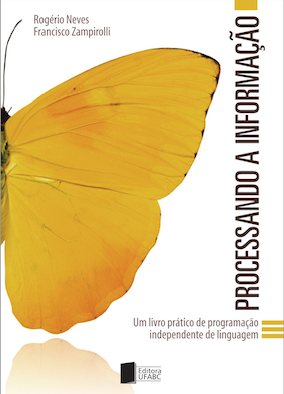
\includegraphics{"figs/Capa_Processando_Informacao.jpg"}

Este caderno (Notebook) é parte complementar \emph{online} do livro
\textbf{\href{https://editora.ufabc.edu.br/matematica-e-ciencias-da-computacao/58-processando-a-informacao}{Processando
a Informação}: um livro prático de programação independente de
linguagem}, que deve ser consultado no caso de dúvidas sobre os temas
apresentados.

\begin{quote}
Este conteúdo pode ser copiado e alterado livremente e foi inspirado
nesse livro.
\end{quote}

    \hypertarget{exercuxedcios}{%
\subsubsection{Exercícios}\label{exercuxedcios}}

    \begin{center}\rule{0.5\linewidth}{0.5pt}\end{center}

\begin{enumerate}
\def\labelenumi{\arabic{enumi}.}
\tightlist
\item
  Demonstre o uso de laços imprimindo os 50 primeiros múltiplos de 3.
\end{enumerate}

    \begin{center}\rule{0.5\linewidth}{0.5pt}\end{center}

\begin{enumerate}
\def\labelenumi{\arabic{enumi}.}
\setcounter{enumi}{1}
\tightlist
\item
  Faça um método \texttt{fibonacci(n)} ou \texttt{F(n)} para retornar o
  Fibonacci \(F(n)\), definido por \(F(0)=0\), \(F(1)=1\), e
  \(\forall n>1\):
\end{enumerate}

\[F(n) = 0, 1, 1, 2, 3, 5, \cdots, F(n-2), F(n-1), F(n-1) + F(n-2) \]

\begin{quote}
Teste em um programa principal várias chamadas destes métodos.
\end{quote}

    \begin{center}\rule{0.5\linewidth}{0.5pt}\end{center}

\begin{enumerate}
\def\labelenumi{\arabic{enumi}.}
\setcounter{enumi}{2}
\tightlist
\item
  Faça um método \texttt{primo(n)} para retornar o valor \texttt{1}
  (número um) se um número \(n\) entrado pelo teclado é primo, caso
  contrário, retornar o valor \texttt{0} (número zero). Isto pode ser
  feito dividindo sucessivamente o número entrado por valores \(i\),
  onde \(i\) varia de \(2\) até \(n-1\), e verificando o resto da
  divisão. Se \(n\%i\) (resto da divisão de \(n\) por \(i\)) for zero
  para qualquer \(i\), o método dever retornar o valor \texttt{0}. Caso
  a condição anterior não ocorra, o método dever retornar o valor
  \texttt{1}.
\end{enumerate}

\begin{quote}
Teste em um programa principal várias chamadas destes métodos, exibindo
a mensagem \texttt{"Não\ é\ primo!"} ou \texttt{"é\ primo"}.
\end{quote}

    \begin{center}\rule{0.5\linewidth}{0.5pt}\end{center}

\begin{enumerate}
\def\labelenumi{\arabic{enumi}.}
\setcounter{enumi}{3}
\tightlist
\item
  Escreva um programa que
\end{enumerate}

\begin{itemize}
\tightlist
\item
  leia três dados: Investimento inicial (I), Taxa de juros (J) e Número
  de meses (N);
\item
  em seguida calcule e exiba uma tabela de juros compostos, com o valor
  total do investimento corrigido do mês zero até o mês selecionado.
\end{itemize}

\begin{quote}
Dica: procure saber mais sobre ``saída formatada'' na linguagem
escolhida. Veja o exemplo de saída produzida usando o comando de
impressão formatada \texttt{print} (python) ou \texttt{printf} (em
diferentes linguagens):
\end{quote}

    \begin{verbatim}
printf("%5d %,20.2f %,20.2f %,20.2f\n", n, Jn, Jt, I );
\end{verbatim}

    \begin{verbatim}
Mês juros no mês    juros total  Investimento
  0      0.00          0.00     100.00
  1      1.00          1.00     101.00
  2     1.51           2.51         102.51
  3     2.02           4.53     104.53
\end{verbatim}

    \begin{center}\rule{0.5\linewidth}{0.5pt}\end{center}

\begin{enumerate}
\def\labelenumi{\arabic{enumi}.}
\setcounter{enumi}{4}
\item
  \begin{enumerate}
  \def\labelenumii{\alph{enumii})}
  \tightlist
  \item
    Utilize laços para calcular o Mínimo Múltiplo Comum (MMC) de dois
    números entrados pelo usuário; b) Faça uma função que receba dois
    números como parâmetros e retorne o MMC ao ponto de chamada.
  \end{enumerate}
\end{enumerate}

    \hypertarget{processando-a-informauxe7uxe3o-cap.-4-estruturas-de-repetiuxe7uxe3o-lauxe7os---pruxe1tica-2}{%
\subsection{Processando a Informação: Cap. 4: Estruturas de Repetição
(Laços) - Prática
2}\label{processando-a-informauxe7uxe3o-cap.-4-estruturas-de-repetiuxe7uxe3o-lauxe7os---pruxe1tica-2}}

    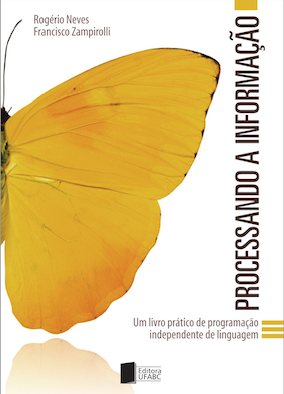
\includegraphics{"figs/Capa_Processando_Informacao.jpg"}

Este caderno (Notebook) é parte complementar \emph{online} do livro
\textbf{\href{https://editora.ufabc.edu.br/matematica-e-ciencias-da-computacao/58-processando-a-informacao}{Processando
a Informação}: um livro prático de programação independente de
linguagem}, que deve ser consultado no caso de dúvidas sobre os temas
apresentados.

\begin{quote}
Este conteúdo pode ser copiado e alterado livremente e foi inspirado
nesse livro.
\end{quote}

    \hypertarget{exercuxedcios}{%
\subsubsection{Exercícios}\label{exercuxedcios}}

Fontes:
\href{https://docente.ifrn.edu.br/jonathanpereira/disciplinas/algoritmos/lista-de-exercicios-estruturas-de-repeticao-1/view}{ref1};
\href{https://www.inf.pucrs.br/flash/cbp/exwhile.html}{ref2};
\href{https://www.inf.pucrs.br/~pinho/LaproI/Exercicios/Repeticao/Lista1.htm}{ref3};
\href{https://pessoal.dainf.ct.utfpr.edu.br/leoneloalmeida/cursos/if71a-s83-2016-01/algoritmos_3_exerc.pdf}{ref4}

    \begin{center}\rule{0.5\linewidth}{0.5pt}\end{center}

\begin{enumerate}
\def\labelenumi{\arabic{enumi}.}
\tightlist
\item
  Desenvolver um algoritmo que leia a altura de 15 pessoas. Este
  programa deverá calcular e mostrar :
\end{enumerate}

\begin{enumerate}
\def\labelenumi{\alph{enumi}.}
\item
  A menor altura do grupo;
\item
  A maior altura do grupo;
\end{enumerate}

    \begin{center}\rule{0.5\linewidth}{0.5pt}\end{center}

\begin{enumerate}
\def\labelenumi{\arabic{enumi}.}
\setcounter{enumi}{1}
\tightlist
\item
  Escrever um algoritmo que leia uma quantidade desconhecida de números
  e conte quantos deles estão em cada um dos seguintes intervalos:
  {[}0-25{]}, {[}26-50{]}, {[}51-75{]} e {[}76-100{]}. A entrada de
  dados deve terminar quando for lido um número negativo.
\end{enumerate}

    \begin{center}\rule{0.5\linewidth}{0.5pt}\end{center}

\begin{enumerate}
\def\labelenumi{\arabic{enumi}.}
\setcounter{enumi}{2}
\tightlist
\item
  Escrever um algoritmo que gera e escreve os números ímpares entre 100
  e 200. Utilizar o método definido da lista anterior (Prática 1).
\end{enumerate}

    \begin{center}\rule{0.5\linewidth}{0.5pt}\end{center}

\begin{enumerate}
\def\labelenumi{\arabic{enumi}.}
\setcounter{enumi}{3}
\tightlist
\item
  Escreva um algoritmo que leia um valor inicial \(a_1\) e uma razão
  \(r\) e imprima uma sequência em P.A. contendo 10 valores.
  Relembrando:
\end{enumerate}

\[a_n = a_1 + (n-1)r\]

    \begin{center}\rule{0.5\linewidth}{0.5pt}\end{center}

\begin{enumerate}
\def\labelenumi{\arabic{enumi}.}
\setcounter{enumi}{4}
\tightlist
\item
  Escreva um algoritmo que leia um valor inicial \(a_1\) e uma razão
  \(q\) e imprima uma sequência em P.G. contendo 10 valores.
  Relembrando:
\end{enumerate}

\[a_n = a_1q^{n-1}\]

    \begin{center}\rule{0.5\linewidth}{0.5pt}\end{center}

\begin{enumerate}
\def\labelenumi{\arabic{enumi}.}
\setcounter{enumi}{5}
\tightlist
\item
  Escreva um algoritmo que leia um valor inicial A e imprima a sequência
  de valores do cálculo de A! e o seu resultado. Formatar a saída
  exatamente como no exemplo:
\end{enumerate}

\[5! = 5 X 4 X 3 X 2 X 1 = 120\]

    \begin{center}\rule{0.5\linewidth}{0.5pt}\end{center}

\begin{enumerate}
\def\labelenumi{\arabic{enumi}.}
\setcounter{enumi}{6}
\tightlist
\item
  Foi feita uma pesquisa entre os habitantes de uma região e coletados
  os dados de altura e sexo (0=masc, 1=fem) das pessoas. Faça um
  programa que leia 50 dados diferentes e informe:
\end{enumerate}

\begin{itemize}
\tightlist
\item
  a maior e a menor altura encontradas
\item
  a média de altura das mulheres
\item
  a média de altura da população
\item
  o percentual de homens na população
\end{itemize}

    \begin{center}\rule{0.5\linewidth}{0.5pt}\end{center}

\begin{enumerate}
\def\labelenumi{\arabic{enumi}.}
\setcounter{enumi}{7}
\tightlist
\item
  Rafa tem 1,50 metro e cresce 2 centímetros por ano, enquanto Zé tem
  1,10 metro e cresce 3 centímetros por ano. Construa um algoritmo que
  calcule e imprima quantos anos serão necessários para que Zé seja
  maior que Rafa.
\end{enumerate}

    \begin{center}\rule{0.5\linewidth}{0.5pt}\end{center}

\begin{enumerate}
\def\labelenumi{\arabic{enumi}.}
\setcounter{enumi}{8}
\tightlist
\item
  Em uma eleição presidencial existem quatro candidatos. Os votos são
  informados através de códigos. Os dados utilizados para a contagem dos
  votos obedecem à seguinte codificação:
\end{enumerate}

\begin{itemize}
\item
  1,2,3,4 = voto para os respectivos candidatos;
\item
  5 = voto nulo;
\item
  6 = voto em branco;
\end{itemize}

Elabore um algoritmo que leia o código do candidado em um voto. Calcule
e escreva:

\begin{itemize}
\item
  total de votos para cada candidato;
\item
  total de votos nulos;
\item
  total de votos em branco;
\end{itemize}

Como finalizador do conjunto de votos, tem-se o valor 0.

    \begin{center}\rule{0.5\linewidth}{0.5pt}\end{center}

\begin{enumerate}
\def\labelenumi{\arabic{enumi}.}
\setcounter{enumi}{9}
\tightlist
\item
  Em uma eleição presidencial existem quatro candidatos. Os votos são
  informados através de códigos. Os dados utilizados para a contagem dos
  votos obedecem à seguinte codificação:
\end{enumerate}

\begin{itemize}
\item
  1,2,3,4 = voto para os respectivos candidatos;
\item
  5 = voto nulo;
\item
  6 = voto em branco;
\end{itemize}

Elabore um algoritmo que leia o código do candidado em um voto. Calcule
e escreva:

\begin{itemize}
\item
  total de votos para cada candidato;
\item
  total de votos nulos;
\item
  total de votos em branco;
\end{itemize}

Como finalizador do conjunto de votos, tem-se o valor 0.

    \begin{center}\rule{0.5\linewidth}{0.5pt}\end{center}

\begin{enumerate}
\def\labelenumi{\arabic{enumi}.}
\setcounter{enumi}{10}
\tightlist
\item
  Faça um programa que desenhe na tela losangos ou triângulos utilizando
  somente o caractere ``\%'' (veja exemplos abaixo). O usuário é quem
  escolhe o que deve ser impresso. O usuário também deve ter a opção de
  escolher o tamanho (em linhas) da figura a ser desenhada.
\end{enumerate}

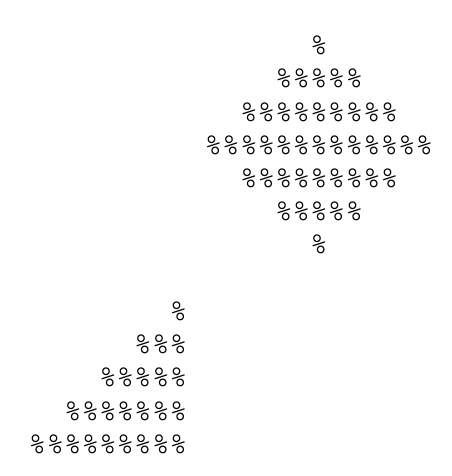
\includegraphics{"figs/cap4ex1.png"}

    \begin{figure}
\centering
\caption{Captura de Tela 2021-06-16 às 14.40.30.png}
\end{figure}

    \begin{center}\rule{0.5\linewidth}{0.5pt}\end{center}

\begin{enumerate}
\def\labelenumi{\arabic{enumi}.}
\setcounter{enumi}{11}
\tightlist
\item
  Construa um algoritmo para o jogo da velha. Esse jogo consiste em um
  tabuleiro de dimensão 3x3 de valores O ou X. Os usuários devem
  informar a linha e a coluna que desejam preencher. A partir da
  terceira jogada de cada jogador é necessário verificar se houve algum
  ganhador. Também é possível que o resultado do jogo seja empate
  (nenhum jogador preencheu uma coluna, uma linha ou uma diagonal).
\end{enumerate}

    \begin{center}\rule{0.5\linewidth}{0.5pt}\end{center}

\begin{enumerate}
\def\labelenumi{\arabic{enumi}.}
\setcounter{enumi}{12}
\tightlist
\item
  Faça um programa que calcule e mostre o maior divisor comum de dois
  números a e b, usando o algoritmo básico de Euclides (temp é uma
  variável inteira, temporária):
\end{enumerate}

\begin{verbatim}
        enquanto b for diferente de 0:
          temp = a
          a = b
          b = temp % b
\end{verbatim}

Esse algoritmo deixará o resultado (MDC) em a, no final.

    \hypertarget{processando-a-informauxe7uxe3o-cap.-4-estruturas-de-repetiuxe7uxe3o-lauxe7os---pruxe1tica-3}{%
\subsection{Processando a Informação: Cap. 4: Estruturas de Repetição
(Laços) - Prática
3}\label{processando-a-informauxe7uxe3o-cap.-4-estruturas-de-repetiuxe7uxe3o-lauxe7os---pruxe1tica-3}}

    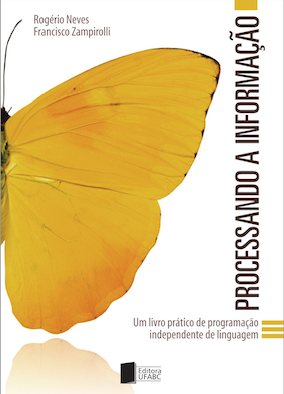
\includegraphics{"figs/Capa_Processando_Informacao.jpg"}

Este caderno (Notebook) é parte complementar \emph{online} do livro
\textbf{\href{https://editora.ufabc.edu.br/matematica-e-ciencias-da-computacao/58-processando-a-informacao}{Processando
a Informação}: um livro prático de programação independente de
linguagem}, que deve ser consultado no caso de dúvidas sobre os temas
apresentados.

\begin{quote}
Este conteúdo pode ser copiado e alterado livremente e foi inspirado
nesse livro.
\end{quote}

    \hypertarget{exercuxedcios}{%
\subsubsection{Exercícios}\label{exercuxedcios}}

Fontes:
\href{https://docente.ifrn.edu.br/jonathanpereira/disciplinas/algoritmos/estruturas-de-repeticao/view}{ref1};
\href{https://www.inf.pucrs.br/~pinho/LaproI/Exercicios/Repeticao/Lista1.htm}{ref2}

    \begin{center}\rule{0.5\linewidth}{0.5pt}\end{center}

\begin{enumerate}
\def\labelenumi{\arabic{enumi}.}
\tightlist
\item
  Escreva um algoritmo que solicite que o usuário entre com valores
  inteiros positivos quaisquer. A condição de parada é digitar um número
  negativo (\(<0\)). Ao final imprima a quantidade de números digitados,
  o somatório dos valores digitados, e a média aritmética do somatório.
\end{enumerate}

    \begin{center}\rule{0.5\linewidth}{0.5pt}\end{center}

\begin{enumerate}
\def\labelenumi{\arabic{enumi}.}
\setcounter{enumi}{1}
\tightlist
\item
  Elabore um algoritmo para fazer cálculo de potenciação. Ou seja,
  \(x^y\). Exemplo: 3\^{}4 = 3 x 3 x 3 x 3. Seu algoritmo deverá
  solicitar que o usuário entre com o valor da base (x) e do expoente
  (y) e apresentar o resultado do cálculo sem utilizar os operadores **
  ou \^{}. Para resolver o problema utilize estrutura de repetição.
\end{enumerate}

    \begin{center}\rule{0.5\linewidth}{0.5pt}\end{center}

\begin{enumerate}
\def\labelenumi{\arabic{enumi}.}
\setcounter{enumi}{2}
\tightlist
\item
  Escreva um algoritmo que calcule a média da seguinte seqüência
  numérica a seguir: \(1/2 + 1/3 + 1/4 + 1/5 + 1/6 + \cdots + 1/50\).
  Feito isto, o algoritmo deverá apresentar uma lista contendo todos os
  números da seqüencia que estão acima da média calculada.
\end{enumerate}

    \begin{center}\rule{0.5\linewidth}{0.5pt}\end{center}

\begin{enumerate}
\def\labelenumi{\arabic{enumi}.}
\setcounter{enumi}{3}
\tightlist
\item
  Apresente o que será impresso na tela do computador pelos algoritmos a
  seguir:
\end{enumerate}

\begin{enumerate}
\def\labelenumi{\alph{enumi})}
\tightlist
\item
  EXEMPLO
\end{enumerate}

\begin{verbatim}
início
 declare J, I, X : inteiro
 J ← 100
 X ← 3
 J ← J + 40
 I ← 5 ^ X * 4
 enquanto (X >= 5) então
  J ← J – 15
  X ← X + 1
  I ← I + X - J
 fim enquanto
 escreva J, I, X
fim 
\end{verbatim}

    \hypertarget{resposta}{%
\paragraph{Resposta:}\label{resposta}}

\begin{longtable}[]{@{}ccc@{}}
\toprule
J & X & I\tabularnewline
\midrule
\endhead
100 & &\tabularnewline
& 3 &\tabularnewline
140 & &\tabularnewline
& & 500\tabularnewline
\bottomrule
\end{longtable}

saída: 140, 500, 3

    \begin{enumerate}
\def\labelenumi{\alph{enumi})}
\setcounter{enumi}{1}
\tightlist
\item
\end{enumerate}

\begin{verbatim}
início
 declare J, I, X : inteiro
 J ← 100
 X ← 3
 J ← J + 40
 I ← 5 ^ X * 4
 repita
  J ← J – 15
  X ← X + 1
  I ← I + X - J
 enquanto (X >= 5)
 escreva J, I, X
fim
\end{verbatim}

    \hypertarget{sua-resposta}{%
\paragraph{Sua Resposta:}\label{sua-resposta}}

\begin{longtable}[]{@{}ccc@{}}
\toprule
J & X & I\tabularnewline
\midrule
\endhead
& &\tabularnewline
\bottomrule
\end{longtable}

    \begin{enumerate}
\def\labelenumi{\alph{enumi})}
\setcounter{enumi}{2}
\tightlist
\item
\end{enumerate}

\begin{verbatim}
início
 declare J, I, X : inteiro
 J ← 100
 X ← 3
 J ← J + 40
 I ← 5 ^ X * 4
 enquanto (X <= 5) faça
  J ← J – 15
  X ← X + 1
  I ← I + X - J
 fim enquanto
 escreva J, I, X
fim 
\end{verbatim}

    \hypertarget{sua-resposta}{%
\paragraph{Sua Resposta:}\label{sua-resposta}}

\begin{longtable}[]{@{}ccc@{}}
\toprule
J & X & I\tabularnewline
\midrule
\endhead
& &\tabularnewline
\bottomrule
\end{longtable}

    \begin{enumerate}
\def\labelenumi{\alph{enumi})}
\setcounter{enumi}{3}
\tightlist
\item
\end{enumerate}

\begin{verbatim}
início
 declare M, N, Y : inteiro
 M ← 10
 Y ← 1
 para N ← 1 até 3 passo 1 faça
  M ← M – 8
  Y ← Y * 3
 fim para
 escreva M, Y, N
fim 
\end{verbatim}

    \hypertarget{sua-resposta}{%
\paragraph{Sua Resposta:}\label{sua-resposta}}

\begin{longtable}[]{@{}ccc@{}}
\toprule
M & N & Y\tabularnewline
\midrule
\endhead
& &\tabularnewline
\bottomrule
\end{longtable}

    \begin{enumerate}
\def\labelenumi{\alph{enumi})}
\setcounter{enumi}{4}
\tightlist
\item
\end{enumerate}

\begin{verbatim}
início
 declare P, Q : inteiro
 declare VALOR : real
 P ← 5
 Q ← P - 8
 VALOR ← 18
 repita
  VALOR ← VALOR + (VALOR * P + Q)
  P ← P + 2
  Q ← Q + 1
 enquanto (Q < 0)
 escreva VALOR
fim 
\end{verbatim}

    \hypertarget{sua-resposta}{%
\paragraph{Sua Resposta:}\label{sua-resposta}}

\begin{longtable}[]{@{}ccc@{}}
\toprule
P & Q & Valor\tabularnewline
\midrule
\endhead
& &\tabularnewline
\bottomrule
\end{longtable}

    \begin{enumerate}
\def\labelenumi{\alph{enumi})}
\setcounter{enumi}{5}
\tightlist
\item
\end{enumerate}

\begin{verbatim}
início
 declare CONT : inteiro
 declare VALOR : real
 declare RESP : caracter
 CONT ← 0
 VALOR ← 0
 RESP ← ‘s’
 enquanto (RESP = ‘s’) faça
  VALOR ← VALOR + 139
  CONT ← CONT + 1
  se (CONT > 3) então
   RESP ← ‘n’
  fim se
 fim enquanto
 escreva VALOR
fim
\end{verbatim}

    \hypertarget{sua-resposta}{%
\paragraph{Sua Resposta:}\label{sua-resposta}}

\begin{longtable}[]{@{}ccc@{}}
\toprule
X & X & X\tabularnewline
\midrule
\endhead
& &\tabularnewline
\bottomrule
\end{longtable}

    \begin{enumerate}
\def\labelenumi{\alph{enumi})}
\setcounter{enumi}{6}
\tightlist
\item
\end{enumerate}

\begin{verbatim}
início
 declare N : inteiro
 declare SOMA : real
 SOMA ← 0
 para N ← 1 até 5 passo 1 faça
  SOMA ← SOMA + 1 / N
 fim para
 escreva SOMA
fim 
\end{verbatim}

    \hypertarget{sua-resposta}{%
\paragraph{Sua Resposta:}\label{sua-resposta}}

\begin{longtable}[]{@{}ccc@{}}
\toprule
X & X & X\tabularnewline
\midrule
\endhead
& &\tabularnewline
\bottomrule
\end{longtable}

    \begin{enumerate}
\def\labelenumi{\alph{enumi})}
\setcounter{enumi}{7}
\tightlist
\item
\end{enumerate}

\begin{verbatim}
início
 declare N : inteiro
 N ← 0
 enquanto (N < 5) faça
  se (N = 0) então
   escreva “Esse número não existe: 1/0”
  senão
  escreva 1 / N
  fim se
  N ← N + 1
 fim enquanto
fim 
\end{verbatim}

    \hypertarget{sua-resposta}{%
\paragraph{Sua Resposta:}\label{sua-resposta}}

\begin{longtable}[]{@{}ccc@{}}
\toprule
X & X & X\tabularnewline
\midrule
\endhead
& &\tabularnewline
\bottomrule
\end{longtable}

    \begin{center}\rule{0.5\linewidth}{0.5pt}\end{center}

\begin{enumerate}
\def\labelenumi{\arabic{enumi}.}
\setcounter{enumi}{4}
\tightlist
\item
  A prefeitura de uma cidade fez uma pesquisa entre seus habitantes,
  coletando dados sobre o salário e número de filhos. A prefeitura
  deseja saber:
\end{enumerate}

\begin{quote}
\begin{enumerate}
\def\labelenumi{\alph{enumi})}
\tightlist
\item
  média do salário da população;
\end{enumerate}
\end{quote}

\begin{quote}
\begin{enumerate}
\def\labelenumi{\alph{enumi})}
\setcounter{enumi}{1}
\tightlist
\item
  média do número de filhos;
\end{enumerate}
\end{quote}

\begin{quote}
\begin{enumerate}
\def\labelenumi{\alph{enumi})}
\setcounter{enumi}{2}
\tightlist
\item
  maior salário;
\end{enumerate}
\end{quote}

\begin{quote}
\begin{enumerate}
\def\labelenumi{\alph{enumi})}
\setcounter{enumi}{3}
\tightlist
\item
  percentual de pessoas com salário até R\$10000,00.
\end{enumerate}
\end{quote}

O final da leitura de dados se dará com a entrada de um salário
negativo. (Use o comando ENQUANTO-FAÇA)

    \begin{center}\rule{0.5\linewidth}{0.5pt}\end{center}

\begin{enumerate}
\def\labelenumi{\arabic{enumi}.}
\setcounter{enumi}{5}
\tightlist
\item
  Escreva um algoritmo que leia o código de um aluno e suas três notas.
  Calcule a média ponderada do aluno, considerando que o peso para a
  maior nota seja 4 e para as duas restantes, 3. Mostre o código do
  aluno, suas três notas, a média calculada e uma mensagem ``APROVADO''
  se a média for maior ou igual a 5 e ``REPROVADO'' se a média for menor
  que 5. Repita a operação até que o código lido seja negativo.
\end{enumerate}

    \begin{center}\rule{0.5\linewidth}{0.5pt}\end{center}

\begin{enumerate}
\def\labelenumi{\arabic{enumi}.}
\setcounter{enumi}{6}
\tightlist
\item
  Escrever um algoritmo que lê um conjunto não determinado de valores,
  um de cada vez, e escreve uma tabela com cabeçalho, que deve ser
  repetido a cada 20 linhas. A tabela conterá o valor lido, seu
  quadrado, seu cubo e sua raiz quadrada.
\end{enumerate}

    \begin{center}\rule{0.5\linewidth}{0.5pt}\end{center}

\begin{enumerate}
\def\labelenumi{\arabic{enumi}.}
\setcounter{enumi}{7}
\tightlist
\item
  Escrever um algoritmo que lê um número não determinado de pares de
  valores m, n, todos inteiros e positivos, um par de cada vez, e
  calcula e escreve a soma dos n inteiros consecutivos a partir de m
  inclusive.
\end{enumerate}

    \begin{center}\rule{0.5\linewidth}{0.5pt}\end{center}

\begin{enumerate}
\def\labelenumi{\arabic{enumi}.}
\setcounter{enumi}{8}
\tightlist
\item
  Escrever um algoritmo que lê um número não determinado de valores para
  m, todos inteiros e positivos, um de cada vez. Se m for par, verificar
  quantos divisores possui e escrever esta informação. Se m for ímpar e
  menor do que 10 calcular e escrever o fatorial de m. Se m for ímpar e
  maior ou igual a 10 calcular e escrever a soma dos inteiros de 1 até
  m.
\end{enumerate}

    \begin{center}\rule{0.5\linewidth}{0.5pt}\end{center}

\begin{enumerate}
\def\labelenumi{\arabic{enumi}.}
\setcounter{enumi}{9}
\tightlist
\item
  Faça um algoritmo que leia uma quantidade não determinada de números
  positivos. Calcule a quantidade de números pares e ímpares, a média de
  valores pares e a média geral dos números lidos. O número que
  encerrará a leitura será zero.
\end{enumerate}

    \begin{center}\rule{0.5\linewidth}{0.5pt}\end{center}

\begin{enumerate}
\def\labelenumi{\arabic{enumi}.}
\setcounter{enumi}{10}
\tightlist
\item
  Foi realizada uma pesquisa de algumas características físicas da
  população de um certa região. Foram entrevistadas 500 pessoas e
  coletados os seguintes dados:
\end{enumerate}

\begin{enumerate}
\def\labelenumi{\alph{enumi})}
\item
  sexo: M (masculino) e F (feminino)
\item
  cor dos olhos: A (azuis), V (verdes) e C (castanhos)
\item
  cor dos cabelos: L (louros), C (castanhos) e P (pretos)
\item
  idade
\end{enumerate}

Deseja-se saber:

a maior idade do grupo a quantidade de indivíduos do sexo feminino, cuja
idade está entre 18 e 35 anos e que tenham olhos verdes e cabelos
louros.

    \begin{center}\rule{0.5\linewidth}{0.5pt}\end{center}

\begin{enumerate}
\def\labelenumi{\arabic{enumi}.}
\setcounter{enumi}{11}
\tightlist
\item
  Foi feita uma estatística nas 200 principais cidades brasileiras para
  coletar dados sobre acidentes de trânsito. Foram obtidos os seguintes
  dados:
\end{enumerate}

\begin{itemize}
\item
  código da cidade
\item
  estado (RS, SC, PR, SP, RJ, \ldots)
\item
  número de veículos de passeio (em 1992)
\item
  número de acidentes de trânsito com vítimas (em 1992)
\end{itemize}

Deseja-se saber:

\begin{enumerate}
\def\labelenumi{\alph{enumi})}
\item
  qual o maior e o menor índice de acidentes de trânsito e a que cidades
  pertencem
\item
  qual a média de veículos nas cidades brasileiras
\item
  qual a média de acidentes com vítimas entre as cidades do Rio Grande
  do Sul.
\end{enumerate}

    \begin{center}\rule{0.5\linewidth}{0.5pt}\end{center}

\begin{enumerate}
\def\labelenumi{\arabic{enumi}.}
\setcounter{enumi}{12}
\tightlist
\item
  Uma loja tem 150 clientes cadastrados e deseja mandar uma
  correspondência a cada um deles anunciando um bônus especial. Escreva
  um algoritmo que leia o nome do cliente e o valor das suas compras no
  ano passado e calcule um bônus de 10\% se o valor das compras for
  menor que 500.000 e de15 \%, caso contrário.
\end{enumerate}

    \begin{center}\rule{0.5\linewidth}{0.5pt}\end{center}

\begin{enumerate}
\def\labelenumi{\arabic{enumi}.}
\setcounter{enumi}{13}
\tightlist
\item
  Faça um algoritmo que mostre os conceitos finais dos alunos de uma
  classe de 75 alunos, considerando (use o comando CASO):
\end{enumerate}

\begin{enumerate}
\def\labelenumi{\alph{enumi})}
\item
  os dados de cada aluno (número de matrícula e nota numérica final)
  serão fornecidos pelo usuário
\item
  a tabela de conceitos segue abaixo:
\end{enumerate}

\begin{longtable}[]{@{}cc@{}}
\toprule
Nota & Conceito\tabularnewline
\midrule
\endhead
de 0,0 a 4,9 & D\tabularnewline
de 5,0 a 6,9 & C\tabularnewline
de 7,0 a 8,9 & B\tabularnewline
de 9,0 a 10,0 & A\tabularnewline
\bottomrule
\end{longtable}

    \hypertarget{processando-a-informauxe7uxe3o-cap.-5-vetores}{%
\section{Processando a Informação: Cap. 5:
Vetores}\label{processando-a-informauxe7uxe3o-cap.-5-vetores}}

    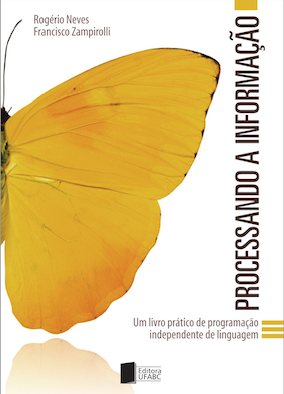
\includegraphics{"figs/Capa_Processando_Informacao.jpg"}

Este caderno (Notebook) é parte complementar \emph{online} do livro
\textbf{\href{https://editora.ufabc.edu.br/matematica-e-ciencias-da-computacao/58-processando-a-informacao}{Processando
a Informação}: um livro prático de programação independente de
linguagem}, que deve ser consultado no caso de dúvidas sobre os temas
apresentados.

\begin{quote}
Este conteúdo pode ser copiado e alterado livremente e foi inspirado
nesse livro.
\end{quote}

    \hypertarget{sumuxe1rio}{%
\subsection{Sumário}\label{sumuxe1rio}}

\begin{itemize}
\tightlist
\item
  Revisão do capítulo anterior
\item
  Introdução
\item
  Trabalhando com vetores
\item
  Acessando elementos de um vetor
\item
  Formas de percorrer um vetor
\item
  Modularização e vetores
\item
  Revisão deste capítulo
\item
  Exercícios
\end{itemize}

    \hypertarget{revisuxe3o-do-capuxedtulo-anterior-estruturas-de-repetiuxe7uxe3o---lauxe7os}{%
\subsection{Revisão do capítulo anterior (Estruturas de Repetição -
Laços)}\label{revisuxe3o-do-capuxedtulo-anterior-estruturas-de-repetiuxe7uxe3o---lauxe7os}}

    \begin{itemize}
\tightlist
\item
  Estruturas de repetição (laços) devem ser utilizadas quando existem
  instruções que se repentem e podem ser de vários tipos, dependendo da
  linguagem utilizada, por exemplo:

  \begin{itemize}
  \tightlist
  \item
    \texttt{do-while} (não aceita em Python)
  \item
    \texttt{while} (a maioria)
  \item
    \texttt{for} (a maioria)
  \item
    \texttt{repeat} (R)
  \end{itemize}
\item
  O uso de laços depende da lógica a ser implementada e da linguagem
  utilizada. Mas, se tiver um número fixo de iterações, geralmente se
  usa \texttt{for}.
\item
  Validação de dados utilizando laços:

  \begin{itemize}
  \tightlist
  \item
    Incluir um laço para verificar o valor lido.
  \end{itemize}
\item
  Interrupção da execução em laços:

  \begin{itemize}
  \tightlist
  \item
    Depende da linguagem, algumas possibilidades:

    \begin{itemize}
    \tightlist
    \item
      \texttt{break} - interrompe o laço
    \item
      \texttt{continue} - não executa o final do laço
    \item
      \texttt{exit} - aborta o laço e o programa!
    \end{itemize}
  \end{itemize}
\item
  Neste capítulo iremos abordar a estrutura de \textbf{Vetor}, incluindo
  os conceitos apresentados nos capítulos anteriores.
\end{itemize}

    \hypertarget{introduuxe7uxe3o}{%
\subsection{Introdução}\label{introduuxe7uxe3o}}

    \begin{itemize}
\tightlist
\item
  Um \textbf{vetor} em programação é formado por um \textbf{conjunto de
  \(n\) variáveis de um mesmo tipo} de dado (em geral), sendo \(n\)
  obrigatoriamente maior que zero.
\item
  Essas variáveis (ou elementos) são identificadas e acessadas por um
  \textbf{nome} e um \textbf{índice}.
\item
  Na maioria das linguagens de programação, o \textbf{índice} recebe
  valores de \(0\) (\textbf{primeiro elemento}) até \(n-1\)
  (\textbf{último elemento}).\\
\item
  As variáveis de um vetor são armazenadas em posições consecutivas de
  memória.
\end{itemize}

    \hypertarget{trabalhando-com-vetores}{%
\subsection{Trabalhando com vetores}\label{trabalhando-com-vetores}}

    \begin{itemize}
\tightlist
\item
  Quando um vetor é criado, é instanciada uma variável do tipo vetor (em
  algumas linguagens de programação, sendo necessário se definir um
  nome, o tipo de dado e o tamanho do vetor).
\item
  Na linguagem C, por exemplo, a definição do tamanho de um vetor ocorre
  antes de compilar o programa.

  \begin{itemize}
  \tightlist
  \item
    Ou seja, o programador deverá informar no código a quantidade de
    memória a ser reservada para o vetor, através de um número inteiro
    positivo ou constante que o contenha, especificando o número de
    elementos do mesmo tipo que a memória reservada irá comportar.
  \item
    Neste caso, uma variável não pode ser usada.
  \end{itemize}
\item
  Já na linguagem Java, é possível alocar memória em tempo de execução
  do programa.

  \begin{itemize}
  \tightlist
  \item
    Por exemplo, é possível criar um vetor para armazenar as notas de
    uma turma de alunos, onde o número de alunos é uma variável a ser
    lida durante a execução do programa.
  \end{itemize}
\end{itemize}

    \begin{itemize}
\tightlist
\item
  Em muitas linguagens, como Java e C, o processo de criar um vetor
  ocorre em dois passos distintos:

  \begin{enumerate}
  \def\labelenumi{\arabic{enumi}.}
  \tightlist
  \item
    primeiro se cria uma variável de referência para o vetor;
  \item
    em seguida se reserva a memória para um dado número de elementos do
    mesmo tipo.
  \end{enumerate}
\item
  No exemplo da figura abaixo,

  \begin{itemize}
  \tightlist
  \item
    a criação da variável de referência de um vetor \texttt{v} define
    apenas a posição de memória em hexadecimal \texttt{0A}, onde será
    armazenado o seu primeiro elemento.

    \begin{itemize}
    \tightlist
    \item
      neste exemplo, \texttt{V{[}0{]}\ =\ -128} é o primeiro elemento do
      vetor.
    \item
      a quantidade de \texttt{bytes} por elemento vai depender to tipo
      de dado armazenado. Neste exemplo cada elemento ocupa um
      \texttt{byte}.
    \end{itemize}
  \item
    o segundo passo da criação de um vetor é reservar (ou alocar)
    memória para todos os seus elementos (dependendo da linguagem).
    \textgreater{} essa alocação de memória pode ocorrer em tempo de
    execução, como ocorre em Python!
  \end{itemize}
\end{itemize}

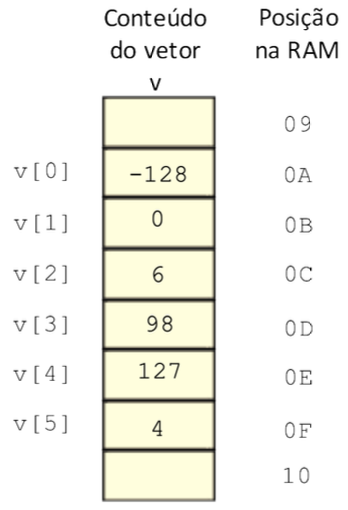
\includegraphics{"figs/image33.png"}

    \begin{figure}
\centering
\caption{image.png}
\end{figure}

    \begin{itemize}
\tightlist
\item
  Note que a variável \texttt{v} acima agora se refere a uma posição de
  memória e não a um elemento de dado.
\item
  Os elementos devem ser acessados através do índice, um por vez.
\item
  Isso pode requerer uso de laços para leitura e impressão dos seus
  elementos, dependendo da linguagem de programação utilizada.

  \begin{itemize}
  \tightlist
  \item
    O índice de vetor é sempre um número inteiro.
  \end{itemize}
\end{itemize}

    \hypertarget{exemplo-01---lerescrever-vetor}{%
\subsection{Exemplo 01 - Ler/Escrever
vetor}\label{exemplo-01---lerescrever-vetor}}

    \hypertarget{pseudocuxf3digo}{%
\paragraph{Pseudocódigo}\label{pseudocuxf3digo}}

    \begin{verbatim}
Instanciar o vetor v1 de inteiro com tamanho 5 // ou
vetor v2 = vetor de inteiros com 100 elementos // ou ainda
vetor v3 = inteiro(10)
v1 = {4,1,10,2,3} // atribuindo valores a v1
\end{verbatim}

    \textbf{Exemplo 01:} Ler uma lista com \texttt{n} alunos com \texttt{RA}
e \texttt{Nome} e escrever formatando a saída como no exemplo:

    \begin{verbatim}
LISTA DE ALUNOS
Número RA     Nome
1      2134   Maria Campos
2      346    João Silva
\end{verbatim}

    \hypertarget{casos-para-teste-moodlevpl}{%
\paragraph{Casos para Teste
Moodle+VPL}\label{casos-para-teste-moodlevpl}}

Para o professor criar uma atividade VPL no Moodle para este Exemplo 01,
basta incluir em \texttt{Casos\ para\ teste}, o seguinte texto (pode
incluir mais casos):

\begin{verbatim}
case=caso1
input=2
2345
9870
Maria Campos
João Silva
output= 
LISTA DE ALUNOS
Número RA     Nota
1      2345   Maria Campos
2      9870   João Silva
\end{verbatim}

    \begin{tcolorbox}[breakable, size=fbox, boxrule=1pt, pad at break*=1mm,colback=cellbackground, colframe=cellborder]
\prompt{In}{incolor}{ }{\boxspacing}
\begin{Verbatim}[commandchars=\\\{\}]
\PY{o}{\PYZpc{}\PYZpc{}writefile} cap5ex01.c
\PY{c+c1}{\PYZsh{}include \PYZlt{}stdio.h\PYZgt{}}

\PY{n+nb}{int} \PY{n}{main}\PY{p}{(}\PY{n}{void}\PY{p}{)} \PY{p}{\PYZob{}}

  \PY{o}{/}\PY{o}{/} \PY{n}{ENTRADA} \PY{n}{DE} \PY{n}{DADOS}
  \PY{n+nb}{int} \PY{n+nb}{max} \PY{o}{=} \PY{l+m+mi}{100}\PY{p}{;} \PY{o}{/}\PY{o}{/} \PY{n}{considerar} \PY{n}{sempre} \PY{n}{um} \PY{n}{número} \PY{n}{grande}
  \PY{n+nb}{int} \PY{n}{n}\PY{p}{,} \PY{n}{ra}\PY{p}{[}\PY{n+nb}{max}\PY{p}{]}\PY{p}{;}     \PY{o}{/}\PY{o}{/} \PY{n}{aloca} \PY{l+m+mi}{100} \PY{n}{ra}\PY{l+s+s1}{\PYZsq{}}\PY{l+s+s1}{s}
  \PY{n}{char} \PY{n}{nome}\PY{p}{[}\PY{n+nb}{max}\PY{p}{]}\PY{p}{[}\PY{l+m+mi}{40}\PY{p}{]}\PY{p}{;} \PY{o}{/}\PY{o}{/} \PY{n}{aloca} \PY{l+m+mi}{100} \PY{n}{nomes} \PY{n}{de} \PY{n}{até} \PY{l+m+mi}{40} \PY{n}{caracteres} \PY{n}{cada}

  \PY{n}{printf}\PY{p}{(}\PY{l+s+s2}{\PYZdq{}}\PY{l+s+s2}{Digite o numero de alunos: }\PY{l+s+s2}{\PYZdq{}}\PY{p}{)}\PY{p}{;}
  \PY{n}{scanf}\PY{p}{(}\PY{l+s+s2}{\PYZdq{}}\PY{l+s+si}{\PYZpc{}d}\PY{l+s+s2}{\PYZdq{}}\PY{p}{,} \PY{o}{\PYZam{}}\PY{n}{n}\PY{p}{)}\PY{p}{;}
  \PY{k}{for} \PY{p}{(}\PY{n+nb}{int} \PY{n}{i} \PY{o}{=} \PY{l+m+mi}{0}\PY{p}{;} \PY{n}{i} \PY{o}{\PYZlt{}} \PY{n}{n}\PY{p}{;} \PY{n}{i}\PY{o}{+}\PY{o}{+}\PY{p}{)} \PY{p}{\PYZob{}}
    \PY{n}{printf}\PY{p}{(}\PY{l+s+s2}{\PYZdq{}}\PY{l+s+s2}{RA: }\PY{l+s+s2}{\PYZdq{}}\PY{p}{)}\PY{p}{;}
    \PY{n}{scanf}\PY{p}{(}\PY{l+s+s2}{\PYZdq{}}\PY{l+s+si}{\PYZpc{}d}\PY{l+s+s2}{\PYZdq{}}\PY{p}{,} \PY{o}{\PYZam{}}\PY{n}{ra}\PY{p}{[}\PY{n}{i}\PY{p}{]}\PY{p}{)}\PY{p}{;}
    \PY{n}{printf}\PY{p}{(}\PY{l+s+s2}{\PYZdq{}}\PY{l+s+s2}{Nome: }\PY{l+s+s2}{\PYZdq{}}\PY{p}{)}\PY{p}{;}
    \PY{n}{scanf}\PY{p}{(}\PY{l+s+s2}{\PYZdq{}}\PY{l+s+si}{\PYZpc{}s}\PY{l+s+s2}{\PYZdq{}}\PY{p}{,} \PY{n}{nome}\PY{p}{[}\PY{n}{i}\PY{p}{]}\PY{p}{)}\PY{p}{;} \PY{o}{/}\PY{o}{/} \PY{n}{ATENÇÃO}\PY{p}{:} \PY{n}{NÃO} \PY{n}{ACEITA} \PY{n}{NOME} \PY{n}{COM} \PY{n}{ESPAÇOS} \PY{n}{e} \PY{n}{NÃO} \PY{n}{USA} \PY{o}{\PYZam{}}
  \PY{p}{\PYZcb{}}
  \PY{o}{/}\PY{o}{/} \PY{n}{PROCESSAMENTO} \PY{err}{?}
  \PY{o}{/}\PY{o}{/} \PY{n}{SAÍDA}
  \PY{n}{printf}\PY{p}{(}\PY{l+s+s2}{\PYZdq{}}\PY{l+s+s2}{LISTA DE ALUNOS}\PY{l+s+se}{\PYZbs{}n}\PY{l+s+s2}{Número}\PY{l+s+se}{\PYZbs{}t}\PY{l+s+s2}{ RA}\PY{l+s+se}{\PYZbs{}t}\PY{l+s+s2}{ Nome}\PY{l+s+se}{\PYZbs{}n}\PY{l+s+s2}{\PYZdq{}}\PY{p}{)}\PY{p}{;}
  \PY{k}{for} \PY{p}{(}\PY{n+nb}{int} \PY{n}{i} \PY{o}{=} \PY{l+m+mi}{0}\PY{p}{;} \PY{n}{i} \PY{o}{\PYZlt{}} \PY{n}{n}\PY{p}{;} \PY{n}{i}\PY{o}{+}\PY{o}{+}\PY{p}{)} \PY{p}{\PYZob{}}
    \PY{n}{printf}\PY{p}{(}\PY{l+s+s2}{\PYZdq{}}\PY{l+s+si}{\PYZpc{}d}\PY{l+s+se}{\PYZbs{}t}\PY{l+s+s2}{ }\PY{l+s+si}{\PYZpc{}d}\PY{l+s+se}{\PYZbs{}t}\PY{l+s+s2}{ }\PY{l+s+si}{\PYZpc{}s}\PY{l+s+se}{\PYZbs{}n}\PY{l+s+s2}{\PYZdq{}}\PY{p}{,} \PY{n}{i} \PY{o}{+} \PY{l+m+mi}{1}\PY{p}{,} \PY{n}{ra}\PY{p}{[}\PY{n}{i}\PY{p}{]}\PY{p}{,} \PY{n}{nome}\PY{p}{[}\PY{n}{i}\PY{p}{]}\PY{p}{)}\PY{p}{;}
  \PY{p}{\PYZcb{}}
  \PY{k}{return} \PY{l+m+mi}{0}\PY{p}{;}
\PY{p}{\PYZcb{}}
\end{Verbatim}
\end{tcolorbox}

    \begin{tcolorbox}[breakable, size=fbox, boxrule=1pt, pad at break*=1mm,colback=cellbackground, colframe=cellborder]
\prompt{In}{incolor}{ }{\boxspacing}
\begin{Verbatim}[commandchars=\\\{\}]
\PY{o}{\PYZpc{}\PYZpc{}}\PY{k}{shell}
gcc \PYZhy{}Wall \PYZhy{}std=c99 cap5ex01.c \PYZhy{}o output2
./output2
\end{Verbatim}
\end{tcolorbox}

    \begin{itemize}
\tightlist
\item
  As \emph{strings} em C têm um último caracter
  \texttt{\textquotesingle{}\textbackslash{}0\textquotesingle{}}. Assim,
  \texttt{s1=s2} e tem três carateres cada:

  \begin{itemize}
  \tightlist
  \item
    \texttt{char\ s1{[}{]}\ =\ "oi";} ou
  \item
    \texttt{char\ s2{[}{]}\ =\ \{\textquotesingle{}o\textquotesingle{},\textquotesingle{}i\textquotesingle{},\textquotesingle{}\textbackslash{}0\textquotesingle{}\};}
  \end{itemize}
\item
  Para ler uma \emph{string} com espaços
  {[}\href{https://www.geeksforgeeks.org/gets-is-risky-to-use}{ref}{]}:
\end{itemize}

    \begin{tcolorbox}[breakable, size=fbox, boxrule=1pt, pad at break*=1mm,colback=cellbackground, colframe=cellborder]
\prompt{In}{incolor}{ }{\boxspacing}
\begin{Verbatim}[commandchars=\\\{\}]
\PY{o}{\PYZpc{}\PYZpc{}writefile} cap5ex01teste.c
\PY{c+c1}{\PYZsh{}include \PYZlt{}stdio.h\PYZgt{}}
\PY{c+c1}{\PYZsh{}include \PYZlt{}string.h\PYZgt{}}

\PY{n+nb}{int} \PY{n}{main}\PY{p}{(}\PY{p}{)} \PY{p}{\PYZob{}}
   \PY{n}{char} \PY{n}{s}\PY{p}{[}\PY{l+m+mi}{40}\PY{p}{]}\PY{p}{;}
   \PY{n}{printf}\PY{p}{(}\PY{l+s+s2}{\PYZdq{}}\PY{l+s+s2}{digite algo:}\PY{l+s+se}{\PYZbs{}n}\PY{l+s+s2}{\PYZdq{}}\PY{p}{)}\PY{p}{;}
   \PY{n}{fgets}\PY{p}{(}\PY{n}{s}\PY{p}{,} \PY{l+m+mi}{40}\PY{p}{,} \PY{n}{stdin}\PY{p}{)}\PY{p}{;}
   \PY{n}{printf}\PY{p}{(}\PY{l+s+s2}{\PYZdq{}}\PY{l+s+s2}{saida: }\PY{l+s+se}{\PYZbs{}\PYZdq{}}\PY{l+s+si}{\PYZpc{}s}\PY{l+s+se}{\PYZbs{}\PYZdq{}}\PY{l+s+s2}{ tamanho: }\PY{l+s+si}{\PYZpc{}ld}\PY{l+s+se}{\PYZbs{}n}\PY{l+s+s2}{\PYZdq{}}\PY{p}{,} \PY{n}{s}\PY{p}{,} \PY{n}{strlen}\PY{p}{(}\PY{n}{s}\PY{p}{)}\PY{p}{)}\PY{p}{;}
   \PY{n}{s}\PY{p}{[}\PY{n}{strlen}\PY{p}{(}\PY{n}{s}\PY{p}{)}\PY{o}{\PYZhy{}}\PY{l+m+mi}{1}\PY{p}{]} \PY{o}{=} \PY{l+s+s1}{\PYZsq{}}\PY{l+s+se}{\PYZbs{}0}\PY{l+s+s1}{\PYZsq{}}\PY{p}{;} \PY{o}{/}\PY{o}{/} \PY{n}{substituir} \PYZbs{}\PY{n}{n} \PY{n}{por} \PYZbs{}\PY{l+m+mi}{0}
   \PY{n}{printf}\PY{p}{(}\PY{l+s+s2}{\PYZdq{}}\PY{l+s+s2}{saida: }\PY{l+s+se}{\PYZbs{}\PYZdq{}}\PY{l+s+si}{\PYZpc{}s}\PY{l+s+se}{\PYZbs{}\PYZdq{}}\PY{l+s+s2}{ tamanho: }\PY{l+s+si}{\PYZpc{}ld}\PY{l+s+se}{\PYZbs{}n}\PY{l+s+s2}{\PYZdq{}}\PY{p}{,} \PY{n}{s}\PY{p}{,} \PY{n}{strlen}\PY{p}{(}\PY{n}{s}\PY{p}{)}\PY{p}{)}\PY{p}{;}
   \PY{k}{return} \PY{l+m+mi}{0}\PY{p}{;}
\PY{p}{\PYZcb{}}
\end{Verbatim}
\end{tcolorbox}

    \begin{tcolorbox}[breakable, size=fbox, boxrule=1pt, pad at break*=1mm,colback=cellbackground, colframe=cellborder]
\prompt{In}{incolor}{ }{\boxspacing}
\begin{Verbatim}[commandchars=\\\{\}]
\PY{o}{\PYZpc{}\PYZpc{}}\PY{k}{shell}
gcc \PYZhy{}Wall \PYZhy{}std=c99 cap5ex01teste.c \PYZhy{}o cap5ex01teste
./cap5ex01teste
\end{Verbatim}
\end{tcolorbox}

    Algumas funções da biblioteca padrão \textbf{string.h}:

\begin{longtable}[]{@{}ll@{}}
\toprule
função & descrição\tabularnewline
\midrule
\endhead
strcopy(s1,s2) & copia s1 em s2\tabularnewline
strcat(s1,s2) & copia s2 no final de s1\tabularnewline
strlen(s) & tamanho de s\tabularnewline
strcmp(s1,s2) & 0 se s1=s2; negativo se s1\textless s2; positivo se
s1\textgreater s2\tabularnewline
strchr(s,ch) & ponteiro para a primeira ocorrência de ch em
s\tabularnewline
strstr(s1,s2) & ponteiro para a primeira ocorrência de s2 em
s1\tabularnewline
\bottomrule
\end{longtable}

    \hypertarget{formas-de-percorrer-um-vetor}{%
\subsection{Formas de Percorrer um
Vetor}\label{formas-de-percorrer-um-vetor}}

    \hypertarget{percorrer-um-vetor-com-o-lauxe7o-para}{%
\subsubsection{\texorpdfstring{Percorrer um vetor com o laço
\texttt{para}}{Percorrer um vetor com o laço para}}\label{percorrer-um-vetor-com-o-lauxe7o-para}}

    \begin{itemize}
\tightlist
\item
  Como um vetor, após criado (alocado e com elementos), tem tamanho fixo
  (sempre com número de elementos \texttt{n\textgreater{}0}), geralmente
  é indicado usar estruturas de repetição do tipo \texttt{para}
  (\texttt{for}), de forma a percorrer todos os elementos do vetor

  \begin{itemize}
  \tightlist
  \item
    assim tornando o código genérico para um vetor de qualquer tamanho
    \texttt{n}.
  \end{itemize}
\item
  Além disso, é natural percorrer (ou varrer) o vetor da posição
  \texttt{i=0} até a posição \texttt{i\textless{}n}

  \begin{itemize}
  \tightlist
  \item
    O índice \texttt{i} assume automaticamente os valores \texttt{0},
    \texttt{1}, \texttt{2}, até \texttt{n-1}, em cada iteração do
    laço.\\
  \item
    Em algumas linguagens, como Matlab e R, o índice assume valores
    entre \texttt{1} até \texttt{n}.
  \end{itemize}
\end{itemize}

    \begin{itemize}
\tightlist
\item
  No exemplo a seguir em pseudocódigo, um vetor \texttt{v} é criado com
  6 posições e o laço \texttt{para} inicializa todos os seus elementos
  com o valor 0.
\item
  A forma natural de percorrer os elementos de um vertou (ou
  \textbf{varrendo} o vetor) é na ordem \textbf{raster}, do primeiro até
  o último elemento.
\item
  A vantagem de se usar a estrutura \texttt{para} para varrer um vertor
  é permitir embutir na própria sintaxe (linha) da instrução:

  \begin{itemize}
  \tightlist
  \item
    declaração e inicialização do índice,
  \item
    incremento e
  \item
    condição de saída do laço.
  \end{itemize}
\end{itemize}

    \hypertarget{pseudocuxf3digo}{%
\paragraph{Pseudocódigo}\label{pseudocuxf3digo}}

    \begin{verbatim}
Instanciar um vetor v de inteiro com 6 elementos (n=6)
para cada indice i, de i=0; até i<n; passo i=i+1 faça
    v[i] = 0
\end{verbatim}

    \hypertarget{percorrer-um-vetor-com-o-lauxe7o-enquanto}{%
\subsubsection{\texorpdfstring{Percorrer um vetor com o laço
\texttt{enquanto}}{Percorrer um vetor com o laço enquanto}}\label{percorrer-um-vetor-com-o-lauxe7o-enquanto}}

    \begin{itemize}
\tightlist
\item
  Se o programador preferir, ou o problema a ser resolvido exigir, o
  vetor pode alternativamente ser percorrido utilizando-se uma estrutura
  de repetição do tipo \texttt{enquanto}:
\end{itemize}

    \hypertarget{pseudocuxf3digo}{%
\paragraph{Pseudocódigo}\label{pseudocuxf3digo}}

    \begin{verbatim}
n=6
vetor v de inteiros com n elementos 
inteiro i=0
enquanto i<n faça {
    v[i] = 0
    i=i+1
}
\end{verbatim}

    \begin{itemize}
\tightlist
\item
  O código usando a estrutura de repetição \texttt{enquanto} produz o
  mesmo resultado que usando com \texttt{para}, porém, usando mais
  instruções:

  \begin{itemize}
  \tightlist
  \item
    a criação do contador \texttt{i}
  \item
    o incremento \texttt{i=i+1}.
  \end{itemize}
\item
  Essas duas instruções ficam encapsuladas na própria instrução
  \texttt{para}.
\end{itemize}

    \hypertarget{outras-formas-de-percorrer-um-vetor}{%
\subsubsection{Outras formas de percorrer um
vetor}\label{outras-formas-de-percorrer-um-vetor}}

    \begin{itemize}
\tightlist
\item
  Dependendo do problema a ser tratado, existem várias formas de se
  varrer um vetor usando estruturas de repetição para acessar cada
  elemento.
\item
  Por exemplo, é possível percorrer o vetor do último elemento para o
  primeiro (essa varradora é chamada de \textbf{anti-raster}):
\end{itemize}

    \hypertarget{pseudocuxf3digo-percorrer-um-vetor-usando-para-na-ordem-inversa-anti-raster.}{%
\paragraph{\texorpdfstring{Pseudocódigo: percorrer um vetor usando para
na ordem inversa
(\textbf{anti-raster}).}{Pseudocódigo: percorrer um vetor usando para na ordem inversa (anti-raster).}}\label{pseudocuxf3digo-percorrer-um-vetor-usando-para-na-ordem-inversa-anti-raster.}}

    \begin{verbatim}
Instanciar um vetor v de inteiro com 6 elementos (n=6)
para cada indice i, de i=n-1; até i<=0; passo i=i-1 faça
    v[i] = 0
\end{verbatim}

    \begin{itemize}
\tightlist
\item
  Também, é possível percorrer somente alguns elementos do vetor, como
  para acessar os elementos que estão nos índices pares ou ímpares,
  diferenciadamente:
\end{itemize}

    \hypertarget{pseudocuxf3digo-percorrer-um-vetor-usando-para-com-passo-2.}{%
\paragraph{\texorpdfstring{Pseudocódigo: percorrer um vetor usando
\texttt{para}, com passo
2.}{Pseudocódigo: percorrer um vetor usando para, com passo 2.}}\label{pseudocuxf3digo-percorrer-um-vetor-usando-para-com-passo-2.}}

    \begin{verbatim}
vetor v de inteiro com 6 elementos
n=6
para cada indice i, de i=0; até i<n-1; passo i=i+2 faça {
    v[i] = 0
    v[i+1] = 1
}
\end{verbatim}

    \hypertarget{modularizauxe7uxe3o-e-vetores}{%
\subsection{Modularização e
Vetores}\label{modularizauxe7uxe3o-e-vetores}}

    \begin{itemize}
\tightlist
\item
  Como uma boa prática de programação, além de comentar os códigos e
  organizar com tabulação, como apresentado nos exemplos deste livro,

  \begin{itemize}
  \tightlist
  \item
    também é recomendável modularizar o código usando métodos, como
    apresentado no Capítulo 2.
  \end{itemize}
\item
  Todo sistema computadorizado de informação possui três partes bem
  definidas, agrupadas em

  \begin{itemize}
  \tightlist
  \item
    módulo(s) de entrada,
  \item
    módulo(s) de processamento e
  \item
    módulo(s) de saída.
  \end{itemize}
\item
  Ao manipular informações armazenadas em vetores, é natural criar
  também pelo menos três módulos ou métodos:

  \begin{itemize}
  \tightlist
  \item
    \texttt{leiaVetor},
  \item
    \texttt{processaVetor} e
  \item
    \texttt{escrevaVetor},
  \end{itemize}

  satisfazendo essa definição de sistema de informação.
\end{itemize}

\begin{quote}
Para a reutilização de código, os módulos \texttt{leiaVetor} e
\texttt{escrevaVetor} poderão ser muito reutilizados para resolver
outros problemas de manipulação de vetores.
\end{quote}

    \hypertarget{pseudocuxf3digo-muxe9todo-para-ler-um-vetor-de-inteiro-tamanho-n.}{%
\paragraph{Pseudocódigo: método para ler um vetor de inteiro tamanho
n.}\label{pseudocuxf3digo-muxe9todo-para-ler-um-vetor-de-inteiro-tamanho-n.}}

    \begin{verbatim}
método leiaVetor(inteiro n): retorna vetor de inteiro v[]
    vetor v de inteiros com n elementos
    para cada índice i, de i=0; até i<n; passo i=i+1 faça
        v[i] = leia("Entre com o elemento " + i + ":");
    retorne v
\end{verbatim}

    \hypertarget{pseudocuxf3digo-muxe9todo-para-escrever-um-vetor-de-inteiro-tamanho-n.}{%
\paragraph{Pseudocódigo: método para escrever um vetor de inteiro
tamanho
n.}\label{pseudocuxf3digo-muxe9todo-para-escrever-um-vetor-de-inteiro-tamanho-n.}}

    \begin{verbatim}
método escrevaVetor(inteiro v[], inteiro n):
    para cada índice i, de i=0; até i<n; passo i=i+1 faça
        escreva(" " + v[i]);
\end{verbatim}

    \hypertarget{pseudocuxf3digo-aplicauxe7uxe3o-de-vetor-usando-muxf3dulos.}{%
\paragraph{Pseudocódigo: aplicação de vetor usando
módulos.}\label{pseudocuxf3digo-aplicauxe7uxe3o-de-vetor-usando-muxf3dulos.}}

    \begin{verbatim}
// Instâncias e Atribuições
inteiro n = leia("Digite o tamanho do vetor:");

// ENTRADA
inteiro v1[] = leiaVetor(n)

// PROCESSAMENTO
// ?

// SAÍDA
escrevaVetor(v2, n)
\end{verbatim}

    \hypertarget{exemplo-02---aplicauxe7uxe3o-simples-1-usando-vetor}{%
\subsection{Exemplo 02 - Aplicação simples 1 usando
vetor}\label{exemplo-02---aplicauxe7uxe3o-simples-1-usando-vetor}}

Considere um algoritmo para ler a quantidade \texttt{n} de alunos de uma
turma. Ler uma lista com \texttt{n} RA's de alunos. Em seguida, ler
também uma lista com \texttt{n} notas de alunos. Como saída do
algoritmo, escrever a seguinte saída.

\begin{verbatim}
LISTA DE ALUNOS
Número RA     Nota
1      2134   9
2      346    7
\end{verbatim}

Utilizar os métodos \texttt{leiaVetor} e \texttt{escrevaVetor}, se
necessários.

    Pseudocódigo

\begin{verbatim}
// ENTRADAS:
// instâncias e atribuições
real media, somador = 0
inteiro contador = 0

// leitura do número de alunos = tamanho do vetor
inteiro n = leia("Digite o número de alunos:");

inteiro ras[] = leiaVetor(n)
inteiro notas[] = leiaVetor(n)
 
// PROCESSAMENTO
// ?

// SAÍDAS:
escreva("LISTA DE ALUNOS")
escreva("Número RA     Nota")
para cada indice i, de i=0; até i<n; passo i=i+1 faça 
    escreva(i+1,"\t",ras[i],"\t",notas[i]
\end{verbatim}

    \hypertarget{casos-para-teste-moodlevpl}{%
\paragraph{Casos para Teste
Moodle+VPL}\label{casos-para-teste-moodlevpl}}

Para o professor criar uma atividade VPL no Moodle para este Exemplo 02,
basta incluir em \texttt{Casos\ para\ teste}, o seguinte texto (pode
incluir mais casos):

\begin{verbatim}
case=caso1
input=2
3456
2345
5
2
output= 
LISTA DE ALUNOS
Número   RA Nota
1    3456    5
2    2345    2
\end{verbatim}

    \begin{tcolorbox}[breakable, size=fbox, boxrule=1pt, pad at break*=1mm,colback=cellbackground, colframe=cellborder]
\prompt{In}{incolor}{ }{\boxspacing}
\begin{Verbatim}[commandchars=\\\{\}]
\PY{o}{\PYZpc{}\PYZpc{}writefile} cap5ex02.c
\PY{c+c1}{\PYZsh{}include \PYZlt{}stdio.h\PYZgt{}}

\PY{n+nb}{int} \PY{n}{main}\PY{p}{(}\PY{n}{void}\PY{p}{)} \PY{p}{\PYZob{}}

  \PY{o}{/}\PY{o}{/} \PY{n}{ENTRADA} \PY{n}{DE} \PY{n}{DADOS}
  \PY{n+nb}{int} \PY{n+nb}{max} \PY{o}{=} \PY{l+m+mi}{100}\PY{p}{;} \PY{o}{/}\PY{o}{/} \PY{n}{número} \PY{n}{máximo} \PY{n}{de} \PY{n}{alunos}
  \PY{n+nb}{int} \PY{n}{n}\PY{p}{,} \PY{n}{ras}\PY{p}{[}\PY{n+nb}{max}\PY{p}{]}\PY{p}{,} \PY{n}{notas}\PY{p}{[}\PY{n+nb}{max}\PY{p}{]}\PY{p}{;}   \PY{o}{/}\PY{o}{/} \PY{n}{variaveis} \PY{n}{de} \PY{n}{referência} \PY{n}{ras} \PY{n}{e} \PY{n}{notas}

  \PY{n}{printf}\PY{p}{(}\PY{l+s+s2}{\PYZdq{}}\PY{l+s+s2}{Digite o numero de alunos: }\PY{l+s+se}{\PYZbs{}n}\PY{l+s+s2}{\PYZdq{}}\PY{p}{)}\PY{p}{;}
  \PY{n}{scanf}\PY{p}{(}\PY{l+s+s2}{\PYZdq{}}\PY{l+s+si}{\PYZpc{}d}\PY{l+s+s2}{\PYZdq{}}\PY{p}{,} \PY{o}{\PYZam{}}\PY{n}{n}\PY{p}{)}\PY{p}{;}

  \PY{n}{printf}\PY{p}{(}\PY{l+s+s2}{\PYZdq{}}\PY{l+s+s2}{RAs: }\PY{l+s+se}{\PYZbs{}n}\PY{l+s+s2}{\PYZdq{}}\PY{p}{)}\PY{p}{;}
  \PY{k}{for} \PY{p}{(}\PY{n+nb}{int} \PY{n}{i} \PY{o}{=} \PY{l+m+mi}{0}\PY{p}{;} \PY{n}{i} \PY{o}{\PYZlt{}} \PY{n}{n}\PY{p}{;} \PY{n}{i}\PY{o}{+}\PY{o}{+}\PY{p}{)} \PY{p}{\PYZob{}}
    \PY{n}{printf}\PY{p}{(}\PY{l+s+s2}{\PYZdq{}}\PY{l+s+s2}{RA }\PY{l+s+si}{\PYZpc{}d}\PY{l+s+s2}{: }\PY{l+s+se}{\PYZbs{}n}\PY{l+s+s2}{\PYZdq{}}\PY{p}{,} \PY{n}{i} \PY{o}{+} \PY{l+m+mi}{1}\PY{p}{)}\PY{p}{;}
    \PY{n}{scanf}\PY{p}{(}\PY{l+s+s2}{\PYZdq{}}\PY{l+s+si}{\PYZpc{}d}\PY{l+s+s2}{\PYZdq{}}\PY{p}{,} \PY{o}{\PYZam{}}\PY{n}{ras}\PY{p}{[}\PY{n}{i}\PY{p}{]}\PY{p}{)}\PY{p}{;}
  \PY{p}{\PYZcb{}}

  \PY{n}{printf}\PY{p}{(}\PY{l+s+s2}{\PYZdq{}}\PY{l+s+s2}{Notas: }\PY{l+s+se}{\PYZbs{}n}\PY{l+s+s2}{\PYZdq{}}\PY{p}{)}\PY{p}{;}
  \PY{k}{for} \PY{p}{(}\PY{n+nb}{int} \PY{n}{i} \PY{o}{=} \PY{l+m+mi}{0}\PY{p}{;} \PY{n}{i} \PY{o}{\PYZlt{}} \PY{n}{n}\PY{p}{;} \PY{n}{i}\PY{o}{+}\PY{o}{+}\PY{p}{)} \PY{p}{\PYZob{}}
    \PY{n}{printf}\PY{p}{(}\PY{l+s+s2}{\PYZdq{}}\PY{l+s+s2}{Nota }\PY{l+s+si}{\PYZpc{}d}\PY{l+s+s2}{: }\PY{l+s+se}{\PYZbs{}n}\PY{l+s+s2}{\PYZdq{}}\PY{p}{,} \PY{n}{i} \PY{o}{+} \PY{l+m+mi}{1}\PY{p}{)}\PY{p}{;}
    \PY{n}{scanf}\PY{p}{(}\PY{l+s+s2}{\PYZdq{}}\PY{l+s+si}{\PYZpc{}d}\PY{l+s+s2}{\PYZdq{}}\PY{p}{,} \PY{o}{\PYZam{}}\PY{n}{notas}\PY{p}{[}\PY{n}{i}\PY{p}{]}\PY{p}{)}\PY{p}{;}
  \PY{p}{\PYZcb{}}

  \PY{o}{/}\PY{o}{/} \PY{n}{PROCESSAMENTO} \PY{err}{?}
  \PY{o}{/}\PY{o}{/} \PY{n}{SAÍDA}
  \PY{n}{printf}\PY{p}{(}\PY{l+s+s2}{\PYZdq{}}\PY{l+s+s2}{LISTA DE ALUNOS}\PY{l+s+se}{\PYZbs{}n}\PY{l+s+s2}{Número}\PY{l+s+se}{\PYZbs{}t}\PY{l+s+s2}{ RA}\PY{l+s+se}{\PYZbs{}t}\PY{l+s+s2}{ Nota}\PY{l+s+se}{\PYZbs{}n}\PY{l+s+s2}{\PYZdq{}}\PY{p}{)}\PY{p}{;}
  \PY{k}{for} \PY{p}{(}\PY{n+nb}{int} \PY{n}{i} \PY{o}{=} \PY{l+m+mi}{0}\PY{p}{;} \PY{n}{i} \PY{o}{\PYZlt{}} \PY{n}{n}\PY{p}{;} \PY{n}{i}\PY{o}{+}\PY{o}{+}\PY{p}{)} \PY{p}{\PYZob{}}
    \PY{n}{printf}\PY{p}{(}\PY{l+s+s2}{\PYZdq{}}\PY{l+s+si}{\PYZpc{}d}\PY{l+s+se}{\PYZbs{}t}\PY{l+s+s2}{ }\PY{l+s+si}{\PYZpc{}d}\PY{l+s+se}{\PYZbs{}t}\PY{l+s+s2}{ }\PY{l+s+si}{\PYZpc{}d}\PY{l+s+se}{\PYZbs{}n}\PY{l+s+s2}{\PYZdq{}}\PY{p}{,} \PY{n}{i} \PY{o}{+} \PY{l+m+mi}{1}\PY{p}{,} \PY{n}{ras}\PY{p}{[}\PY{n}{i}\PY{p}{]}\PY{p}{,} \PY{n}{notas}\PY{p}{[}\PY{n}{i}\PY{p}{]}\PY{p}{)}\PY{p}{;}
  \PY{p}{\PYZcb{}}
  \PY{k}{return} \PY{l+m+mi}{0}\PY{p}{;}
\PY{p}{\PYZcb{}}
\end{Verbatim}
\end{tcolorbox}

    \begin{tcolorbox}[breakable, size=fbox, boxrule=1pt, pad at break*=1mm,colback=cellbackground, colframe=cellborder]
\prompt{In}{incolor}{ }{\boxspacing}
\begin{Verbatim}[commandchars=\\\{\}]
\PY{o}{\PYZpc{}\PYZpc{}}\PY{k}{shell}
gcc \PYZhy{}Wall \PYZhy{}std=c99 cap5ex02.c \PYZhy{}o output2
./output2
\end{Verbatim}
\end{tcolorbox}

    Existem várias formas de usar vetor em métodos:

\begin{itemize}
\tightlist
\item
  como argumento:

  \begin{itemize}
  \tightlist
  \item
    \texttt{void\ metodo\ (int\ *v,\ int\ n)\ \{...\}}
  \item
    \texttt{void\ metodo\ (int\ v{[}{]},\ int\ n)\ \{...\}}
  \item
    \texttt{void\ metodo\ (int\ v{[}max{]},\ int\ n)\ \{...\}}
  \end{itemize}
\item
  como retorno:

  \begin{itemize}
  \tightlist
  \item
    \texttt{int\ *\ metodo\ (int\ n)\ \{...\}} - alocar vetor dentro do
    método, alocação dinâmica de memória.
  \end{itemize}
\end{itemize}

    \begin{tcolorbox}[breakable, size=fbox, boxrule=1pt, pad at break*=1mm,colback=cellbackground, colframe=cellborder]
\prompt{In}{incolor}{ }{\boxspacing}
\begin{Verbatim}[commandchars=\\\{\}]
\PY{o}{\PYZpc{}\PYZpc{}writefile} cap5ex02teste1.c
\PY{c+c1}{\PYZsh{}include \PYZlt{}stdio.h\PYZgt{}}

\PY{c+c1}{\PYZsh{}define MAX\PYZus{}ALUNOS 20 // número máximo de alunos}

\PY{n}{void} \PY{n}{leiaVetor}\PY{p}{(}\PY{n+nb}{int} \PY{o}{*}\PY{n}{v}\PY{p}{,} \PY{n+nb}{int} \PY{n}{n}\PY{p}{)} \PY{p}{\PYZob{}}
  \PY{k}{for} \PY{p}{(}\PY{n+nb}{int} \PY{n}{i} \PY{o}{=} \PY{l+m+mi}{0}\PY{p}{;} \PY{n}{i} \PY{o}{\PYZlt{}} \PY{n}{n}\PY{p}{;} \PY{n}{i}\PY{o}{+}\PY{o}{+}\PY{p}{)} 
    \PY{n}{scanf}\PY{p}{(}\PY{l+s+s2}{\PYZdq{}}\PY{l+s+si}{\PYZpc{}d}\PY{l+s+s2}{\PYZdq{}}\PY{p}{,} \PY{o}{\PYZam{}}\PY{n}{v}\PY{p}{[}\PY{n}{i}\PY{p}{]}\PY{p}{)}\PY{p}{;}
\PY{p}{\PYZcb{}}

\PY{n+nb}{int} \PY{n}{main}\PY{p}{(}\PY{n}{void}\PY{p}{)} \PY{p}{\PYZob{}}

  \PY{o}{/}\PY{o}{/} \PY{n}{ENTRADA} \PY{n}{DE} \PY{n}{DADOS}
  \PY{n+nb}{int} \PY{n}{n}\PY{p}{,} \PY{n}{ras}\PY{p}{[}\PY{n}{MAX\PYZus{}ALUNOS}\PY{p}{]}\PY{p}{,} \PY{n}{notas}\PY{p}{[}\PY{n}{MAX\PYZus{}ALUNOS}\PY{p}{]}\PY{p}{;}   \PY{o}{/}\PY{o}{/} \PY{n}{variaveis} \PY{n}{de} \PY{n}{referência} \PY{n}{ras} \PY{n}{e} \PY{n}{notas}

  \PY{n}{printf}\PY{p}{(}\PY{l+s+s2}{\PYZdq{}}\PY{l+s+s2}{Digite o numero de alunos: }\PY{l+s+se}{\PYZbs{}n}\PY{l+s+s2}{\PYZdq{}}\PY{p}{)}\PY{p}{;}
  \PY{n}{scanf}\PY{p}{(}\PY{l+s+s2}{\PYZdq{}}\PY{l+s+si}{\PYZpc{}d}\PY{l+s+s2}{\PYZdq{}}\PY{p}{,} \PY{o}{\PYZam{}}\PY{n}{n}\PY{p}{)}\PY{p}{;}

  \PY{n}{printf}\PY{p}{(}\PY{l+s+s2}{\PYZdq{}}\PY{l+s+s2}{RAs: }\PY{l+s+se}{\PYZbs{}n}\PY{l+s+s2}{\PYZdq{}}\PY{p}{)}\PY{p}{;}
  \PY{n}{leiaVetor}\PY{p}{(}\PY{n}{ras}\PY{p}{,} \PY{n}{n}\PY{p}{)}\PY{p}{;}

  \PY{n}{printf}\PY{p}{(}\PY{l+s+s2}{\PYZdq{}}\PY{l+s+s2}{Notas: }\PY{l+s+se}{\PYZbs{}n}\PY{l+s+s2}{\PYZdq{}}\PY{p}{)}\PY{p}{;}
  \PY{n}{leiaVetor}\PY{p}{(}\PY{n}{notas}\PY{p}{,} \PY{n}{n}\PY{p}{)}\PY{p}{;}

  \PY{o}{/}\PY{o}{/} \PY{n}{PROCESSAMENTO} \PY{err}{?}
  \PY{o}{/}\PY{o}{/} \PY{n}{SAÍDA}
  \PY{n}{printf}\PY{p}{(}\PY{l+s+s2}{\PYZdq{}}\PY{l+s+s2}{LISTA DE ALUNOS}\PY{l+s+se}{\PYZbs{}n}\PY{l+s+s2}{Número}\PY{l+s+se}{\PYZbs{}t}\PY{l+s+s2}{ RA}\PY{l+s+se}{\PYZbs{}t}\PY{l+s+s2}{ Nota}\PY{l+s+se}{\PYZbs{}n}\PY{l+s+s2}{\PYZdq{}}\PY{p}{)}\PY{p}{;}
  \PY{k}{for} \PY{p}{(}\PY{n+nb}{int} \PY{n}{i} \PY{o}{=} \PY{l+m+mi}{0}\PY{p}{;} \PY{n}{i} \PY{o}{\PYZlt{}} \PY{n}{n}\PY{p}{;} \PY{n}{i}\PY{o}{+}\PY{o}{+}\PY{p}{)} 
    \PY{n}{printf}\PY{p}{(}\PY{l+s+s2}{\PYZdq{}}\PY{l+s+si}{\PYZpc{}d}\PY{l+s+se}{\PYZbs{}t}\PY{l+s+s2}{ }\PY{l+s+si}{\PYZpc{}d}\PY{l+s+se}{\PYZbs{}t}\PY{l+s+s2}{ }\PY{l+s+si}{\PYZpc{}d}\PY{l+s+se}{\PYZbs{}n}\PY{l+s+s2}{\PYZdq{}}\PY{p}{,} \PY{n}{i} \PY{o}{+} \PY{l+m+mi}{1}\PY{p}{,} \PY{n}{ras}\PY{p}{[}\PY{n}{i}\PY{p}{]}\PY{p}{,} \PY{n}{notas}\PY{p}{[}\PY{n}{i}\PY{p}{]}\PY{p}{)}\PY{p}{;}
  
  \PY{k}{return} \PY{l+m+mi}{0}\PY{p}{;}
\PY{p}{\PYZcb{}}
\end{Verbatim}
\end{tcolorbox}

    \begin{tcolorbox}[breakable, size=fbox, boxrule=1pt, pad at break*=1mm,colback=cellbackground, colframe=cellborder]
\prompt{In}{incolor}{ }{\boxspacing}
\begin{Verbatim}[commandchars=\\\{\}]
\PY{o}{\PYZpc{}\PYZpc{}}\PY{k}{shell}
gcc \PYZhy{}Wall \PYZhy{}std=c99 cap5ex02teste1.c \PYZhy{}o output2
./output2
\end{Verbatim}
\end{tcolorbox}

    \begin{tcolorbox}[breakable, size=fbox, boxrule=1pt, pad at break*=1mm,colback=cellbackground, colframe=cellborder]
\prompt{In}{incolor}{ }{\boxspacing}
\begin{Verbatim}[commandchars=\\\{\}]
\PY{o}{\PYZpc{}\PYZpc{}writefile} cap5ex02teste2.c
\PY{c+c1}{\PYZsh{}include \PYZlt{}stdio.h\PYZgt{}}
\PY{c+c1}{\PYZsh{}include \PYZlt{}stdlib.h\PYZgt{}  // malloc e free}

\PY{n+nb}{int} \PY{o}{*} \PY{n}{leiaVetor}\PY{p}{(}\PY{n+nb}{int} \PY{n}{n}\PY{p}{)} \PY{p}{\PYZob{}}
  \PY{n+nb}{int} \PY{o}{*}\PY{n}{v}\PY{o}{=} \PY{n}{malloc}\PY{p}{(}\PY{n}{sizeof}\PY{p}{(}\PY{n}{n}\PY{p}{)}\PY{p}{)}\PY{p}{;}  \PY{o}{/}\PY{o}{/} \PY{n}{ALOCAÇÃO} \PY{n}{DINÂMICA}
  \PY{k}{for} \PY{p}{(}\PY{n+nb}{int} \PY{n}{i} \PY{o}{=} \PY{l+m+mi}{0}\PY{p}{;} \PY{n}{i} \PY{o}{\PYZlt{}} \PY{n}{n}\PY{p}{;} \PY{n}{i}\PY{o}{+}\PY{o}{+}\PY{p}{)} \PY{p}{\PYZob{}}
    \PY{n}{scanf}\PY{p}{(}\PY{l+s+s2}{\PYZdq{}}\PY{l+s+si}{\PYZpc{}d}\PY{l+s+s2}{\PYZdq{}}\PY{p}{,} \PY{o}{\PYZam{}}\PY{n}{v}\PY{p}{[}\PY{n}{i}\PY{p}{]}\PY{p}{)}\PY{p}{;} 
  \PY{p}{\PYZcb{}}
  \PY{k}{return} \PY{n}{v}\PY{p}{;}
\PY{p}{\PYZcb{}}

\PY{n+nb}{int} \PY{n}{main}\PY{p}{(}\PY{n}{void}\PY{p}{)} \PY{p}{\PYZob{}}

  \PY{o}{/}\PY{o}{/} \PY{n}{ENTRADA} \PY{n}{DE} \PY{n}{DADOS}
  \PY{n+nb}{int} \PY{n}{n}\PY{p}{,} \PY{o}{*}\PY{n}{ras}\PY{p}{,} \PY{o}{*}\PY{n}{notas}\PY{p}{;}   \PY{o}{/}\PY{o}{/} \PY{n}{variaveis} \PY{n}{de} \PY{n}{referência} \PY{n}{ras} \PY{n}{e} \PY{n}{notas}

  \PY{n}{printf}\PY{p}{(}\PY{l+s+s2}{\PYZdq{}}\PY{l+s+s2}{Digite o numero de alunos: }\PY{l+s+s2}{\PYZdq{}}\PY{p}{)}\PY{p}{;}
  \PY{n}{scanf}\PY{p}{(}\PY{l+s+s2}{\PYZdq{}}\PY{l+s+si}{\PYZpc{}d}\PY{l+s+s2}{\PYZdq{}}\PY{p}{,} \PY{o}{\PYZam{}}\PY{n}{n}\PY{p}{)}\PY{p}{;}

  \PY{n}{printf}\PY{p}{(}\PY{l+s+s2}{\PYZdq{}}\PY{l+s+s2}{RAs: }\PY{l+s+s2}{\PYZdq{}}\PY{p}{)}\PY{p}{;}
  \PY{n}{ras} \PY{o}{=} \PY{n}{leiaVetor}\PY{p}{(}\PY{n}{n}\PY{p}{)}\PY{p}{;}

  \PY{n}{printf}\PY{p}{(}\PY{l+s+s2}{\PYZdq{}}\PY{l+s+s2}{Notas: }\PY{l+s+s2}{\PYZdq{}}\PY{p}{)}\PY{p}{;}
  \PY{n}{notas} \PY{o}{=} \PY{n}{leiaVetor}\PY{p}{(}\PY{n}{n}\PY{p}{)}\PY{p}{;}

  \PY{o}{/}\PY{o}{/} \PY{n}{PROCESSAMENTO} \PY{err}{?}
  \PY{o}{/}\PY{o}{/} \PY{n}{SAÍDA}
  \PY{n}{printf}\PY{p}{(}\PY{l+s+s2}{\PYZdq{}}\PY{l+s+s2}{LISTA DE ALUNOS}\PY{l+s+se}{\PYZbs{}n}\PY{l+s+s2}{Número}\PY{l+s+se}{\PYZbs{}t}\PY{l+s+s2}{ RA}\PY{l+s+se}{\PYZbs{}t}\PY{l+s+s2}{ Nota}\PY{l+s+se}{\PYZbs{}n}\PY{l+s+s2}{\PYZdq{}}\PY{p}{)}\PY{p}{;}
  \PY{k}{for} \PY{p}{(}\PY{n+nb}{int} \PY{n}{i} \PY{o}{=} \PY{l+m+mi}{0}\PY{p}{;} \PY{n}{i} \PY{o}{\PYZlt{}} \PY{n}{n}\PY{p}{;} \PY{n}{i}\PY{o}{+}\PY{o}{+}\PY{p}{)} \PY{p}{\PYZob{}}
      \PY{n}{printf}\PY{p}{(}\PY{l+s+s2}{\PYZdq{}}\PY{l+s+si}{\PYZpc{}d}\PY{l+s+se}{\PYZbs{}t}\PY{l+s+s2}{ }\PY{l+s+si}{\PYZpc{}d}\PY{l+s+se}{\PYZbs{}t}\PY{l+s+s2}{ }\PY{l+s+si}{\PYZpc{}d}\PY{l+s+se}{\PYZbs{}n}\PY{l+s+s2}{\PYZdq{}}\PY{p}{,}\PY{n}{i}\PY{o}{+}\PY{l+m+mi}{1}\PY{p}{,} \PY{n}{ras}\PY{p}{[}\PY{n}{i}\PY{p}{]}\PY{p}{,}\PY{n}{notas}\PY{p}{[}\PY{n}{i}\PY{p}{]}\PY{p}{)}\PY{p}{;}
  \PY{p}{\PYZcb{}}
  \PY{n}{free}\PY{p}{(}\PY{n}{ras}\PY{p}{)}\PY{p}{;}   \PY{o}{/}\PY{o}{/} \PY{n}{LIBERAR} \PY{n}{MEMÓRIA} \PY{n}{ALOCADA} \PY{n}{COM} \PY{n}{malloc}
  \PY{n}{free}\PY{p}{(}\PY{n}{notas}\PY{p}{)}\PY{p}{;}
  \PY{k}{return} \PY{l+m+mi}{0}\PY{p}{;}
\PY{p}{\PYZcb{}}
\end{Verbatim}
\end{tcolorbox}

    \begin{tcolorbox}[breakable, size=fbox, boxrule=1pt, pad at break*=1mm,colback=cellbackground, colframe=cellborder]
\prompt{In}{incolor}{ }{\boxspacing}
\begin{Verbatim}[commandchars=\\\{\}]
\PY{o}{\PYZpc{}\PYZpc{}}\PY{k}{shell}
gcc \PYZhy{}Wall \PYZhy{}std=c99 cap5ex02teste2.c \PYZhy{}o output2
./output2
\end{Verbatim}
\end{tcolorbox}

    \hypertarget{exemplo-03---aplicauxe7uxe3o-simples-2-usando-vetor}{%
\subsection{Exemplo 03 - Aplicação simples 2 usando
vetor}\label{exemplo-03---aplicauxe7uxe3o-simples-2-usando-vetor}}

Considere um algoritmo para ler a quantidade \texttt{n} de alunos de uma
turma. Ler também uma lista com \texttt{n} notas de alunos. Como saída
do algoritmo, escrever a média da turma e quantos alunos ficaram acima
da média.

    Pseudocódigo

\begin{verbatim}
// ENTRADAS:
// instâncias e atribuições
real media, somador = 0
inteiro contador = 0

// leitura do número de alunos = tamanho do vetor
inteiro n = leia("Digite o número de alunos:");

inteiro ras[] = leiaVetor(n)
real notas[] = leiaVetor(n)

// PROCESSAMENTO: soma, média e contador
para cada indice i, de i=0; até i<n; passo i=i+1 faça 
    somador = somador + notas[i] // soma
media = somador / n   // média
para cada indice i, de i=0; até i<n; passo i=i+1 faça    
    se ( notas[i] >= media ) // conta alunos>=media
        contador = contador + 1

// SAÍDAS:
escreva("Média da turma=" + media) // Saída
escreva("Alunos acima da média: " + contador)
escreva("LISTA DE ALUNOS ACIMA DA MÉDIA")
escreva("RA\t Nota")
para cada indice i, de i=0; até i<n; passo i=i+1 faça 
  se (nota[i] >= media)
    escreva(ras[i],"\t",notas[i]
\end{verbatim}

    \hypertarget{casos-para-teste-moodlevpl}{%
\paragraph{Casos para Teste
Moodle+VPL}\label{casos-para-teste-moodlevpl}}

Para o professor criar uma atividade VPL no Moodle para este Exemplo 03,
basta incluir em \texttt{Casos\ para\ teste}, o seguinte texto (pode
incluir mais casos):

\begin{verbatim}
case=caso1
input=2
233245
234534
9
4
output= 
Média da turma = 6.5
Número de alunos acima da média = 1
LISTA DE ALUNOS ACIMA DA MÉDIA
RA      Nota
233245  9
\end{verbatim}

    \begin{tcolorbox}[breakable, size=fbox, boxrule=1pt, pad at break*=1mm,colback=cellbackground, colframe=cellborder]
\prompt{In}{incolor}{ }{\boxspacing}
\begin{Verbatim}[commandchars=\\\{\}]
\PY{o}{\PYZpc{}\PYZpc{}writefile} cap5ex03.c
\PY{c+c1}{\PYZsh{}include \PYZlt{}stdio.h\PYZgt{}}
\PY{c+c1}{\PYZsh{}include \PYZlt{}stdlib.h\PYZgt{}  }

\PY{n+nb}{int} \PY{o}{*} \PY{n}{leiaVetor}\PY{p}{(}\PY{n+nb}{int} \PY{n}{n}\PY{p}{)} \PY{p}{\PYZob{}}
  \PY{n+nb}{int} \PY{o}{*}\PY{n}{v}\PY{o}{=} \PY{n}{malloc}\PY{p}{(}\PY{n}{sizeof}\PY{p}{(}\PY{n}{n}\PY{p}{)}\PY{p}{)}\PY{p}{;}  
  \PY{k}{for} \PY{p}{(}\PY{n+nb}{int} \PY{n}{i} \PY{o}{=} \PY{l+m+mi}{0}\PY{p}{;} \PY{n}{i} \PY{o}{\PYZlt{}} \PY{n}{n}\PY{p}{;} \PY{n}{i}\PY{o}{+}\PY{o}{+}\PY{p}{)} \PY{p}{\PYZob{}}
    \PY{n}{scanf}\PY{p}{(}\PY{l+s+s2}{\PYZdq{}}\PY{l+s+si}{\PYZpc{}d}\PY{l+s+s2}{\PYZdq{}}\PY{p}{,} \PY{o}{\PYZam{}}\PY{n}{v}\PY{p}{[}\PY{n}{i}\PY{p}{]}\PY{p}{)}\PY{p}{;} 
  \PY{p}{\PYZcb{}}
  \PY{k}{return} \PY{n}{v}\PY{p}{;}
\PY{p}{\PYZcb{}}

\PY{n+nb}{int} \PY{n}{main}\PY{p}{(}\PY{n}{void}\PY{p}{)} \PY{p}{\PYZob{}}

  \PY{o}{/}\PY{o}{/} \PY{n}{ENTRADA} \PY{n}{DE} \PY{n}{DADOS}
  \PY{n+nb}{int} \PY{n}{n}\PY{p}{,} \PY{o}{*}\PY{n}{ras}\PY{p}{,} \PY{o}{*}\PY{n}{notas}\PY{p}{;}   \PY{o}{/}\PY{o}{/} \PY{n}{variaveis} \PY{n}{de} \PY{n}{referência} \PY{n}{ras} \PY{n}{e} \PY{n}{notas}
  \PY{n+nb}{float} \PY{n}{media}\PY{p}{,}\PY{n}{somador} \PY{o}{=} \PY{l+m+mf}{0.0}\PY{p}{;}
  \PY{n+nb}{int} \PY{n}{contador} \PY{o}{=} \PY{l+m+mi}{0}\PY{p}{;}

  \PY{n}{printf}\PY{p}{(}\PY{l+s+s2}{\PYZdq{}}\PY{l+s+s2}{Digite o numero de alunos: }\PY{l+s+s2}{\PYZdq{}}\PY{p}{)}\PY{p}{;}
  \PY{n}{scanf}\PY{p}{(}\PY{l+s+s2}{\PYZdq{}}\PY{l+s+si}{\PYZpc{}d}\PY{l+s+s2}{\PYZdq{}}\PY{p}{,} \PY{o}{\PYZam{}}\PY{n}{n}\PY{p}{)}\PY{p}{;}

  \PY{n}{printf}\PY{p}{(}\PY{l+s+s2}{\PYZdq{}}\PY{l+s+s2}{RAs: }\PY{l+s+s2}{\PYZdq{}}\PY{p}{)}\PY{p}{;}
  \PY{n}{ras} \PY{o}{=} \PY{n}{leiaVetor}\PY{p}{(}\PY{n}{n}\PY{p}{)}\PY{p}{;}

  \PY{n}{printf}\PY{p}{(}\PY{l+s+s2}{\PYZdq{}}\PY{l+s+s2}{Notas: }\PY{l+s+s2}{\PYZdq{}}\PY{p}{)}\PY{p}{;}
  \PY{n}{notas} \PY{o}{=} \PY{n}{leiaVetor}\PY{p}{(}\PY{n}{n}\PY{p}{)}\PY{p}{;}

  \PY{o}{/}\PY{o}{/} \PY{n}{PROCESSAMENTO}\PY{p}{:} \PY{n}{soma}\PY{p}{,} \PY{n}{média} \PY{n}{e} \PY{n}{contador}
  \PY{k}{for} \PY{p}{(}\PY{n+nb}{int} \PY{n}{i} \PY{o}{=} \PY{l+m+mi}{0}\PY{p}{;} \PY{n}{i} \PY{o}{\PYZlt{}} \PY{n}{n}\PY{p}{;} \PY{n}{i}\PY{o}{+}\PY{o}{+}\PY{p}{)} \PY{p}{\PYZob{}}
      \PY{n}{somador} \PY{o}{=} \PY{n}{somador} \PY{o}{+} \PY{n}{notas}\PY{p}{[}\PY{n}{i}\PY{p}{]}\PY{p}{;}   \PY{o}{/}\PY{o}{/} \PY{n}{soma}
  \PY{p}{\PYZcb{}}
  \PY{n}{media} \PY{o}{=} \PY{p}{(}\PY{n+nb}{float}\PY{p}{)} \PY{n}{somador} \PY{o}{/} \PY{n}{n}\PY{p}{;}            \PY{o}{/}\PY{o}{/} \PY{n}{média}

  \PY{k}{for} \PY{p}{(}\PY{n+nb}{int} \PY{n}{i} \PY{o}{=} \PY{l+m+mi}{0}\PY{p}{;} \PY{n}{i} \PY{o}{\PYZlt{}} \PY{n}{n}\PY{p}{;} \PY{n}{i}\PY{o}{+}\PY{o}{+}\PY{p}{)} \PY{p}{\PYZob{}}
      \PY{k}{if} \PY{p}{(}\PY{n}{notas}\PY{p}{[}\PY{n}{i}\PY{p}{]} \PY{o}{\PYZgt{}}\PY{o}{=} \PY{n}{media}\PY{p}{)} \PY{p}{\PYZob{}}        \PY{o}{/}\PY{o}{/} \PY{n}{conta} \PY{n}{alunos}\PY{o}{\PYZgt{}}\PY{o}{=}\PY{n}{media}
          \PY{n}{contador} \PY{o}{=} \PY{n}{contador} \PY{o}{+} \PY{l+m+mi}{1}\PY{p}{;}
      \PY{p}{\PYZcb{}}
  \PY{p}{\PYZcb{}}
  \PY{o}{/}\PY{o}{/} \PY{n}{SAÍDA} \PY{n}{DE} \PY{n}{DADOS}
  \PY{n}{printf}\PY{p}{(}\PY{l+s+s2}{\PYZdq{}}\PY{l+s+s2}{Média da turma = }\PY{l+s+si}{\PYZpc{}.1f}\PY{l+s+se}{\PYZbs{}n}\PY{l+s+s2}{\PYZdq{}}\PY{p}{,}\PY{n}{media}\PY{p}{)}\PY{p}{;}
  \PY{n}{printf}\PY{p}{(}\PY{l+s+s2}{\PYZdq{}}\PY{l+s+s2}{Número de alunos acima da média = }\PY{l+s+si}{\PYZpc{}d}\PY{l+s+se}{\PYZbs{}n}\PY{l+s+s2}{\PYZdq{}}\PY{p}{,}\PY{n}{contador}\PY{p}{)}\PY{p}{;}
  \PY{n}{printf}\PY{p}{(}\PY{l+s+s2}{\PYZdq{}}\PY{l+s+s2}{LISTA DE ALUNOS ACIMA DA MÉDIA}\PY{l+s+se}{\PYZbs{}n}\PY{l+s+s2}{RA}\PY{l+s+se}{\PYZbs{}t}\PY{l+s+s2}{ Nota}\PY{l+s+se}{\PYZbs{}n}\PY{l+s+s2}{\PYZdq{}}\PY{p}{)}\PY{p}{;}
  \PY{k}{for} \PY{p}{(}\PY{n+nb}{int} \PY{n}{i} \PY{o}{=} \PY{l+m+mi}{0}\PY{p}{;} \PY{n}{i} \PY{o}{\PYZlt{}} \PY{n}{n}\PY{p}{;} \PY{n}{i}\PY{o}{+}\PY{o}{+}\PY{p}{)} \PY{p}{\PYZob{}}
    \PY{k}{if} \PY{p}{(}\PY{n}{notas}\PY{p}{[}\PY{n}{i}\PY{p}{]} \PY{o}{\PYZgt{}}\PY{o}{=} \PY{n}{media}\PY{p}{)} \PY{p}{\PYZob{}}        \PY{o}{/}\PY{o}{/} \PY{n}{conta} \PY{n}{alunos}\PY{o}{\PYZgt{}}\PY{o}{=}\PY{n}{media}
      \PY{n}{printf}\PY{p}{(}\PY{l+s+s2}{\PYZdq{}}\PY{l+s+si}{\PYZpc{}d}\PY{l+s+se}{\PYZbs{}t}\PY{l+s+s2}{ }\PY{l+s+si}{\PYZpc{}d}\PY{l+s+se}{\PYZbs{}n}\PY{l+s+s2}{\PYZdq{}}\PY{p}{,}\PY{n}{ras}\PY{p}{[}\PY{n}{i}\PY{p}{]}\PY{p}{,}\PY{n}{notas}\PY{p}{[}\PY{n}{i}\PY{p}{]}\PY{p}{)}\PY{p}{;}
    \PY{p}{\PYZcb{}}
  \PY{p}{\PYZcb{}}
  \PY{n}{free}\PY{p}{(}\PY{n}{ras}\PY{p}{)}\PY{p}{;}  \PY{o}{/}\PY{o}{/} \PY{n}{liberar} \PY{n}{memória} \PY{n}{alocado} \PY{n}{com} \PY{n}{malloc}
  \PY{n}{free}\PY{p}{(}\PY{n}{notas}\PY{p}{)}\PY{p}{;}
  \PY{k}{return} \PY{l+m+mi}{0}\PY{p}{;}
\PY{p}{\PYZcb{}}
\end{Verbatim}
\end{tcolorbox}

    \begin{tcolorbox}[breakable, size=fbox, boxrule=1pt, pad at break*=1mm,colback=cellbackground, colframe=cellborder]
\prompt{In}{incolor}{ }{\boxspacing}
\begin{Verbatim}[commandchars=\\\{\}]
\PY{o}{\PYZpc{}\PYZpc{}}\PY{k}{shell}
gcc \PYZhy{}Wall \PYZhy{}std=c99 cap5ex03.c \PYZhy{}o output2
./output2
\end{Verbatim}
\end{tcolorbox}

    \hypertarget{exemplo-04---aplicauxe7uxe3o-dilata-vetor}{%
\subsection{Exemplo 04 - Aplicação ``dilata''
vetor}\label{exemplo-04---aplicauxe7uxe3o-dilata-vetor}}

\begin{itemize}
\item
  O programador deve tomar cuidado ao acessar os elementos de um vetor
  para \textbf{não ultrapassar os seus limites alocados previamente}, ou
  seja,

  \begin{itemize}
  \tightlist
  \item
    para um vetor \texttt{v} de tamanho \texttt{n}, índices \texttt{i}
    com \texttt{i\textless{}0} ou \texttt{i\textgreater{}=n} não
    existem.
  \end{itemize}
\item
  O exemplo a seguir ilustra este problema.
\item
  Considere o problema de ``\textbf{dilatar}'' um vetor.

  \begin{itemize}
  \tightlist
  \item
    O objetivo é criar um vetor \texttt{v1} de inteiros com \texttt{n}
    posições e um outro vetor \texttt{v2} de inteiros também com
    \texttt{n} posições.
  \item
    Cada posição \texttt{i} de \texttt{v2} armazena o cálculo do
    \textbf{máximo} entre cada elemento \texttt{i} em \texttt{v1} e seus
    vizinhos:

    \begin{enumerate}
    \def\labelenumi{\arabic{enumi}.}
    \tightlist
    \item
      à esquerda \texttt{v1{[}i-1{]}},
    \item
      do próprio elemento \texttt{v1{[}i{]}} e
    \item
      do seu vizinho à direita \texttt{v1{[}i+1{]}}.
    \end{enumerate}
  \end{itemize}
\item
  Veja uma ilustração da operação de dilatação na Figura abaixo, onde
  \texttt{v1} é o vetor de entrada e \texttt{v2} é o vetor de saída,
  contendo a ``dilatação'' de \texttt{v1}, seguido do código para
  resolver este problema proposto.
\end{itemize}

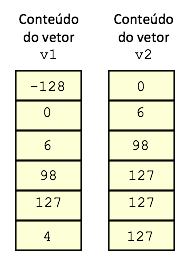
\includegraphics{"figs/image35.png"}

    \begin{figure}
\centering
\caption{image.png}
\end{figure}

    Pseudocódigo

\begin{verbatim}
método escrevaVetor(inteiro v[], inteiro n):
    para cada índice i, de i=0; até i<n; passo i=i+1 faça
        escreva(" " + v[i]);

método leiaVetor(inteiro n): retorna vetor de inteiro v[]
    vetor v de inteiros com n elementos
    para cada índice i, de i=0; até i<n; passo i=i+1 faça
        v[i] = leia("Entre com o elemento " + i + ":");
    retorne v

// Inicializações
inteiro max=0
// ENTRADA
inteiro n = leia("Digite o tamanho do vetor:");
vetores v1 e v2 de inteiros com n elementos

inteiro v1[] = leiaVetor(n)

// PROCESSAMENTO
para cada índice i, de i=0; até i<n; passo i=i+1 faça
    max = v[i]
    se i-1 >= 0 e max < v1[i-1] faça
        max = v1[i-1]
    se i+1 < n e max < v1[i+1] faça
        max = v1[i+1]
    v2[i] = max

// SAÍDA
escrevaVetor(v2)
\end{verbatim}

    \hypertarget{casos-para-teste-moodlevpl}{%
\paragraph{Casos para Teste
Moodle+VPL}\label{casos-para-teste-moodlevpl}}

Para o professor criar uma atividade VPL no Moodle para este Exemplo 04,
basta incluir em \texttt{Casos\ para\ teste}, o seguinte texto (pode
incluir mais casos):

\begin{verbatim}
case=caso1
input=6
-128
0
6
98
127
4
output=v2:
0
6
98
127
127
127
\end{verbatim}

    \begin{tcolorbox}[breakable, size=fbox, boxrule=1pt, pad at break*=1mm,colback=cellbackground, colframe=cellborder]
\prompt{In}{incolor}{ }{\boxspacing}
\begin{Verbatim}[commandchars=\\\{\}]
\PY{o}{\PYZpc{}\PYZpc{}writefile} cap5ex04.c
\PY{c+c1}{\PYZsh{}include \PYZlt{}stdio.h\PYZgt{}}
\PY{c+c1}{\PYZsh{}include \PYZlt{}stdlib.h\PYZgt{}  // malloc e free}

\PY{n+nb}{int} \PY{o}{*} \PY{n}{leiaVetor}\PY{p}{(}\PY{n+nb}{int} \PY{n}{n}\PY{p}{)} \PY{p}{\PYZob{}}
  \PY{n+nb}{int} \PY{o}{*}\PY{n}{v} \PY{o}{=} \PY{n}{malloc}\PY{p}{(}\PY{n}{n}\PY{o}{*}\PY{n}{sizeof}\PY{p}{(}\PY{n+nb}{int}\PY{p}{)}\PY{p}{)}\PY{p}{;} 
  \PY{k}{for} \PY{p}{(}\PY{n+nb}{int} \PY{n}{i} \PY{o}{=} \PY{l+m+mi}{0}\PY{p}{;} \PY{n}{i} \PY{o}{\PYZlt{}} \PY{n}{n}\PY{p}{;} \PY{n}{i}\PY{o}{+}\PY{o}{+}\PY{p}{)} \PY{p}{\PYZob{}}
    \PY{n}{scanf}\PY{p}{(}\PY{l+s+s2}{\PYZdq{}}\PY{l+s+si}{\PYZpc{}d}\PY{l+s+s2}{\PYZdq{}}\PY{p}{,} \PY{o}{\PYZam{}}\PY{n}{v}\PY{p}{[}\PY{n}{i}\PY{p}{]}\PY{p}{)}\PY{p}{;} 
  \PY{p}{\PYZcb{}}
  \PY{k}{return} \PY{n}{v}\PY{p}{;}
\PY{p}{\PYZcb{}}
\PY{n}{void} \PY{n}{escrevaVetor}\PY{p}{(}\PY{n+nb}{int} \PY{o}{*}\PY{n}{v}\PY{p}{,} \PY{n+nb}{int} \PY{n}{n}\PY{p}{)} \PY{p}{\PYZob{}}
  \PY{k}{for} \PY{p}{(}\PY{n+nb}{int} \PY{n}{i} \PY{o}{=} \PY{l+m+mi}{0}\PY{p}{;} \PY{n}{i} \PY{o}{\PYZlt{}} \PY{n}{n}\PY{p}{;} \PY{n}{i}\PY{o}{+}\PY{o}{+}\PY{p}{)} \PY{p}{\PYZob{}}
    \PY{n}{printf}\PY{p}{(}\PY{l+s+s2}{\PYZdq{}}\PY{l+s+si}{\PYZpc{}d}\PY{l+s+se}{\PYZbs{}n}\PY{l+s+s2}{\PYZdq{}}\PY{p}{,} \PY{n}{v}\PY{p}{[}\PY{n}{i}\PY{p}{]}\PY{p}{)}\PY{p}{;} 
  \PY{p}{\PYZcb{}}
\PY{p}{\PYZcb{}}
\PY{n+nb}{int} \PY{n}{main}\PY{p}{(}\PY{n}{void}\PY{p}{)} \PY{p}{\PYZob{}}
  \PY{o}{/}\PY{o}{/} \PY{n}{ENTRADA} \PY{n}{DE} \PY{n}{DADOS}
  \PY{n+nb}{int} \PY{n}{n}\PY{p}{,} \PY{o}{*}\PY{n}{v1}\PY{p}{;}   \PY{o}{/}\PY{o}{/} \PY{n}{variaveis} \PY{n}{de} \PY{n}{referência} \PY{n}{v1}
  \PY{n}{printf}\PY{p}{(}\PY{l+s+s2}{\PYZdq{}}\PY{l+s+s2}{Digite o tamanho do vetor: }\PY{l+s+s2}{\PYZdq{}}\PY{p}{)}\PY{p}{;}
  \PY{n}{scanf}\PY{p}{(}\PY{l+s+s2}{\PYZdq{}}\PY{l+s+si}{\PYZpc{}d}\PY{l+s+s2}{\PYZdq{}}\PY{p}{,} \PY{o}{\PYZam{}}\PY{n}{n}\PY{p}{)}\PY{p}{;}
  \PY{n+nb}{int} \PY{o}{*}\PY{n}{v2} \PY{o}{=} \PY{n}{malloc}\PY{p}{(}\PY{l+m+mi}{100}\PY{o}{*}\PY{n}{sizeof}\PY{p}{(}\PY{n+nb}{int}\PY{p}{)}\PY{p}{)}\PY{p}{;}
  \PY{n}{printf}\PY{p}{(}\PY{l+s+s2}{\PYZdq{}}\PY{l+s+s2}{Digite os elementos: }\PY{l+s+s2}{\PYZdq{}}\PY{p}{)}\PY{p}{;}
  \PY{n}{v1} \PY{o}{=} \PY{n}{leiaVetor}\PY{p}{(}\PY{n}{n}\PY{p}{)}\PY{p}{;}
  \PY{o}{/}\PY{o}{/} \PY{n}{PROCESSAMENTO}
  \PY{k}{for} \PY{p}{(}\PY{n+nb}{int} \PY{n}{i} \PY{o}{=} \PY{l+m+mi}{0}\PY{p}{;} \PY{n}{i} \PY{o}{\PYZlt{}} \PY{n}{n}\PY{p}{;} \PY{n}{i}\PY{o}{+}\PY{o}{+}\PY{p}{)} \PY{p}{\PYZob{}}
    \PY{n+nb}{int} \PY{n+nb}{max} \PY{o}{=} \PY{n}{v1}\PY{p}{[}\PY{n}{i}\PY{p}{]}\PY{p}{;}
    \PY{k}{if} \PY{p}{(}\PY{n}{i}\PY{o}{\PYZhy{}}\PY{l+m+mi}{1} \PY{o}{\PYZgt{}}\PY{o}{=} \PY{l+m+mi}{0} \PY{o}{\PYZam{}}\PY{o}{\PYZam{}} \PY{n+nb}{max} \PY{o}{\PYZlt{}} \PY{n}{v1}\PY{p}{[}\PY{n}{i}\PY{o}{\PYZhy{}}\PY{l+m+mi}{1}\PY{p}{]}\PY{p}{)}
        \PY{n+nb}{max} \PY{o}{=} \PY{n}{v1}\PY{p}{[}\PY{n}{i}\PY{o}{\PYZhy{}}\PY{l+m+mi}{1}\PY{p}{]}\PY{p}{;}
    \PY{k}{if} \PY{p}{(}\PY{n}{i}\PY{o}{+}\PY{l+m+mi}{1} \PY{o}{\PYZlt{}} \PY{n}{n} \PY{o}{\PYZam{}}\PY{o}{\PYZam{}} \PY{n+nb}{max} \PY{o}{\PYZlt{}} \PY{n}{v1}\PY{p}{[}\PY{n}{i}\PY{o}{+}\PY{l+m+mi}{1}\PY{p}{]}\PY{p}{)}
        \PY{n+nb}{max} \PY{o}{=} \PY{n}{v1}\PY{p}{[}\PY{n}{i}\PY{o}{+}\PY{l+m+mi}{1}\PY{p}{]}\PY{p}{;}
    \PY{n}{v2}\PY{p}{[}\PY{n}{i}\PY{p}{]} \PY{o}{=} \PY{n+nb}{max}\PY{p}{;}
  \PY{p}{\PYZcb{}}
  \PY{o}{/}\PY{o}{/} \PY{n}{SAÍDA}\PY{p}{:}
  \PY{n}{printf}\PY{p}{(}\PY{l+s+s2}{\PYZdq{}}\PY{l+s+se}{\PYZbs{}n}\PY{l+s+s2}{v2:}\PY{l+s+se}{\PYZbs{}n}\PY{l+s+s2}{\PYZdq{}}\PY{p}{)}\PY{p}{;}
  \PY{n}{escrevaVetor}\PY{p}{(}\PY{n}{v2}\PY{p}{,}\PY{n}{n}\PY{p}{)}\PY{p}{;}
  \PY{n}{free}\PY{p}{(}\PY{n}{v1}\PY{p}{)}\PY{p}{;} \PY{o}{/}\PY{o}{/} \PY{n}{liberar} \PY{n}{memória} \PY{n}{alocado} \PY{n}{com} \PY{n}{malloc}
  \PY{n}{free}\PY{p}{(}\PY{n}{v2}\PY{p}{)}\PY{p}{;}
  \PY{k}{return} \PY{l+m+mi}{0}\PY{p}{;}
\PY{p}{\PYZcb{}}
\end{Verbatim}
\end{tcolorbox}

    \begin{tcolorbox}[breakable, size=fbox, boxrule=1pt, pad at break*=1mm,colback=cellbackground, colframe=cellborder]
\prompt{In}{incolor}{ }{\boxspacing}
\begin{Verbatim}[commandchars=\\\{\}]
\PY{o}{\PYZpc{}\PYZpc{}}\PY{k}{shell}
gcc \PYZhy{}Wall \PYZhy{}std=c99 cap5ex04.c \PYZhy{}o output2
./output2
\end{Verbatim}
\end{tcolorbox}

    \hypertarget{exercuxedcios}{%
\subsection{Exercícios}\label{exercuxedcios}}

    Ver notebook Colab nos arquivos \texttt{cap5.partX.lab.*.ipynb}
(\texttt{X} \(\in\) \texttt{{[}2,3{]}} e \texttt{*} é a extensão da
linguagem), utilizando alguma linguagem de programação de sua
preferência, organizadas em subpastas contidas de \texttt{"gen"}, na
pasta do Google Drive
\href{https://drive.google.com/drive/folders/1YlFwv8XYN7PYYf-HwDMlkxzbmXzJw9cM?usp=sharing}{colabs}.

    \hypertarget{atividades-no-moodlevpl}{%
\subsection{Atividades no Moodle+VPL}\label{atividades-no-moodlevpl}}

Algumas atividades no Moodle+VPL pedem como entradas vetores de inteiros
(ou reais), \textbf{armazenados em uma única linha}. Exemplo de entrada
a ser lida:

\hypertarget{entrada-de-dados-cada-linha-contem-um-texto-ou-string-incluindo-os-elementos-do-vetor-e-vuxe1rios-espauxe7os}{%
\subsubsection{\texorpdfstring{Entrada de Dados (cada linha contem um
texto ou \emph{string} incluindo os elementos do vetor e vários espaços
``\texttt{}''):}{Entrada de Dados (cada linha contem um texto ou string incluindo os elementos do vetor e vários espaços ``\,''):}}\label{entrada-de-dados-cada-linha-contem-um-texto-ou-string-incluindo-os-elementos-do-vetor-e-vuxe1rios-espauxe7os}}

\begin{verbatim}
7 3 7 9 7 7 0 9 8 4 8 9 0 1 7 8 4 1 1 0 
2 1 9 4 3 6 0 9 8 4 2 8 0 6 7 3 2 4 5 9
\end{verbatim}

Para não ter que incluir várias entradas inteiras, a melhor solução é
fazer um método de leitura, passando como argumento um texto
(\emph{string}) referente a cada linha. Esse método deve retornar o
vetor.

    \begin{tcolorbox}[breakable, size=fbox, boxrule=1pt, pad at break*=1mm,colback=cellbackground, colframe=cellborder]
\prompt{In}{incolor}{ }{\boxspacing}
\begin{Verbatim}[commandchars=\\\{\}]
\PY{o}{\PYZpc{}\PYZpc{}writefile} str2int.c
\PY{c+c1}{\PYZsh{}include \PYZlt{}stdio.h\PYZgt{}}
\PY{c+c1}{\PYZsh{}include \PYZlt{}string.h\PYZgt{}}
\PY{c+c1}{\PYZsh{}include \PYZlt{}stdlib.h\PYZgt{}}

\PY{n+nb}{int} \PY{n}{main}\PY{p}{(}\PY{p}{)} \PY{p}{\PYZob{}}
   \PY{n}{char} \PY{n}{string}\PY{p}{[}\PY{p}{]} \PY{o}{=} \PY{l+s+s2}{\PYZdq{}}\PY{l+s+s2}{7 3 7 9 7 7 0 9 8 4 8 9 0 1     7 8 4 1 1 0     }\PY{l+s+s2}{\PYZdq{}}\PY{p}{;}
   \PY{n}{char} \PY{o}{*} \PY{n}{token} \PY{o}{=} \PY{n}{strtok}\PY{p}{(}\PY{n}{string}\PY{p}{,} \PY{l+s+s2}{\PYZdq{}}\PY{l+s+s2}{ }\PY{l+s+s2}{\PYZdq{}}\PY{p}{)}\PY{p}{;}
   \PY{n+nb}{int} \PY{n}{v}\PY{p}{[}\PY{l+m+mi}{100}\PY{p}{]}\PY{p}{;}
   \PY{n+nb}{int} \PY{n}{i} \PY{o}{=} \PY{l+m+mi}{0}\PY{p}{;}
   \PY{k}{while}\PY{p}{(} \PY{n}{token} \PY{o}{!=} \PY{n}{NULL} \PY{p}{)} \PY{p}{\PYZob{}}
      \PY{n}{v}\PY{p}{[}\PY{n}{i}\PY{o}{+}\PY{o}{+}\PY{p}{]} \PY{o}{=} \PY{n}{atoi}\PY{p}{(}\PY{n}{token}\PY{p}{)}\PY{p}{;} \PY{o}{/}\PY{o}{/} \PY{n}{converte} \PY{n}{texto} \PY{n}{para} \PY{n}{inteiro}
      \PY{n}{token} \PY{o}{=} \PY{n}{strtok}\PY{p}{(}\PY{n}{NULL}\PY{p}{,} \PY{l+s+s2}{\PYZdq{}}\PY{l+s+s2}{ }\PY{l+s+s2}{\PYZdq{}}\PY{p}{)}\PY{p}{;}
   \PY{p}{\PYZcb{}}
   \PY{n+nb}{int} \PY{n}{n}\PY{o}{=}\PY{n}{i}\PY{p}{;}
   \PY{k}{for} \PY{p}{(}\PY{n}{i}\PY{o}{=}\PY{l+m+mi}{0}\PY{p}{;}\PY{n}{i}\PY{o}{\PYZlt{}}\PY{n}{n}\PY{p}{;}\PY{n}{i}\PY{o}{+}\PY{o}{+} \PY{p}{)}\PY{p}{\PYZob{}}
     \PY{n}{printf}\PY{p}{(}\PY{l+s+s2}{\PYZdq{}}\PY{l+s+si}{\PYZpc{}d}\PY{l+s+s2}{ }\PY{l+s+s2}{\PYZdq{}}\PY{p}{,}\PY{n}{v}\PY{p}{[}\PY{n}{i}\PY{p}{]}\PY{p}{)}\PY{p}{;}
   \PY{p}{\PYZcb{}}
   \PY{k}{return} \PY{l+m+mi}{0}\PY{p}{;}
\PY{p}{\PYZcb{}}
\end{Verbatim}
\end{tcolorbox}

    \begin{tcolorbox}[breakable, size=fbox, boxrule=1pt, pad at break*=1mm,colback=cellbackground, colframe=cellborder]
\prompt{In}{incolor}{ }{\boxspacing}
\begin{Verbatim}[commandchars=\\\{\}]
\PY{o}{\PYZpc{}\PYZpc{}}\PY{k}{shell}
gcc \PYZhy{}Wall \PYZhy{}std=c99 str2int.c \PYZhy{}o output2
./output2
\end{Verbatim}
\end{tcolorbox}

    \hypertarget{entrada-de-dados-a-linha-contem-um-texto-ou-string}{%
\subsubsection{\texorpdfstring{Entrada de Dados (a linha contem um texto
ou
\emph{string}):}{Entrada de Dados (a linha contem um texto ou string):}}\label{entrada-de-dados-a-linha-contem-um-texto-ou-string}}

\begin{verbatim}
A UFABC completou 15 anos!
\end{verbatim}

Como contar as vogais de um texto?

    \hypertarget{revisuxe3o-deste-capuxedtulo-de-vetores}{%
\subsection{Revisão deste capítulo de
Vetores}\label{revisuxe3o-deste-capuxedtulo-de-vetores}}

\begin{itemize}
\tightlist
\item
  Introdução \textgreater{} Vetores são estruturas para armazenar vários
  elementos de um mesmo tipo de dados em uma única variável.
\item
  Trabalhando com vetores \textgreater{} Cada linguagem possui uma
  sintaxe própria para declarar e alocar vetores.
\item
  Acessando elementos de um vetor \textgreater{} ATENÇÃO para não
  acessar uma posição do vetor não reservada/alocada, geralmente
  \texttt{\textless{}0} e \texttt{\textgreater{}=n}.
\item
  Formas de percorrer um vetor \textgreater{} É possível varrer um vetor
  na forma \textbf{\emph{raster}} e \textbf{\emph{anti-raster}}, também
  usando diferentes passos, mas geralmente é passo=1.
\item
  Modularização e vetores \textgreater{} Muito útil usar principalmente
  os módulos de \texttt{leiaVetor} e \texttt{escrevaVetor}, podendo ser
  reaproveitados em vários códigos.
\item
  Exercícios
\item
  Revisão deste capítulo de Vetores
\end{itemize}

    \hypertarget{processando-a-informauxe7uxe3o-cap.-5-vetores---pruxe1tica-1}{%
\subsection{Processando a Informação: Cap. 5: Vetores - Prática
1}\label{processando-a-informauxe7uxe3o-cap.-5-vetores---pruxe1tica-1}}

    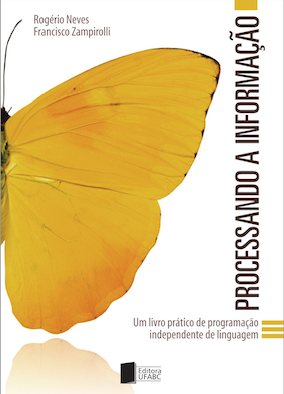
\includegraphics{"figs/Capa_Processando_Informacao.jpg"}

Este caderno (Notebook) é parte complementar \emph{online} do livro
\textbf{\href{https://editora.ufabc.edu.br/matematica-e-ciencias-da-computacao/58-processando-a-informacao}{Processando
a Informação}: um livro prático de programação independente de
linguagem}, que deve ser consultado no caso de dúvidas sobre os temas
apresentados.

\begin{quote}
Este conteúdo pode ser copiado e alterado livremente e foi inspirado
nesse livro.
\end{quote}

    \hypertarget{exercuxedcios}{%
\subsubsection{Exercícios}\label{exercuxedcios}}

{[}ref.: http://tiagodemelo.info/livros/logica/node4.html{]}

    \begin{center}\rule{0.5\linewidth}{0.5pt}\end{center}

\begin{enumerate}
\def\labelenumi{\arabic{enumi}.}
\tightlist
\item
  Criar um vetor para armazenar as notas de uma turma com n alunos e
  imprimir a maior e a menor nota da turma.
\end{enumerate}

    \begin{center}\rule{0.5\linewidth}{0.5pt}\end{center}

\begin{enumerate}
\def\labelenumi{\arabic{enumi}.}
\setcounter{enumi}{1}
\tightlist
\item
  Criar um vetor de inteiros com n elementos. Achar o menor valor e
  mostrar, junto com o número de vezes ele ocorre no vetor.
\end{enumerate}

    \begin{center}\rule{0.5\linewidth}{0.5pt}\end{center}

\begin{enumerate}
\def\labelenumi{\arabic{enumi}.}
\setcounter{enumi}{2}
\tightlist
\item
  Criar um vetor \texttt{v1} de inteiros com \texttt{n} elementos com
  valores de \texttt{0} até \texttt{9}. Criar um outro vetor
  \texttt{v2}, onde os elementos recebam a quantidade de ocorrências dos
  valores de \texttt{0} a \texttt{10}, armazenando nas posições
  \texttt{0} a \texttt{10} de \texttt{v2}.
\end{enumerate}

    \begin{center}\rule{0.5\linewidth}{0.5pt}\end{center}

\begin{enumerate}
\def\labelenumi{\arabic{enumi}.}
\setcounter{enumi}{3}
\tightlist
\item
  Criar um vetor de inteiros com n elementos e uma função que receba um
  vetor e duas posições \texttt{i} e \texttt{j}, efetuando a troca dos
  valores das posições \texttt{i} e \texttt{j} no vetor. Verificar na
  função se \texttt{0\textless{}=i\textless{}n} e
  \texttt{0\textless{}=j\textless{}n} antes de realizar a troca.
\end{enumerate}

    \begin{center}\rule{0.5\linewidth}{0.5pt}\end{center}

\begin{enumerate}
\def\labelenumi{\arabic{enumi}.}
\setcounter{enumi}{4}
\tightlist
\item
  Criar um vetor de inteiros com n elementos e ordenar os seus valores.
\end{enumerate}

Ver simulações de vários algoritmos de ordenação:
\href{https://www.toptal.com/developers/sorting-algorithms}{link}

    \hypertarget{processando-a-informauxe7uxe3o-cap.-5-vetores---pruxe1tica-2}{%
\subsection{Processando a Informação: Cap. 5: Vetores - Prática
2}\label{processando-a-informauxe7uxe3o-cap.-5-vetores---pruxe1tica-2}}

    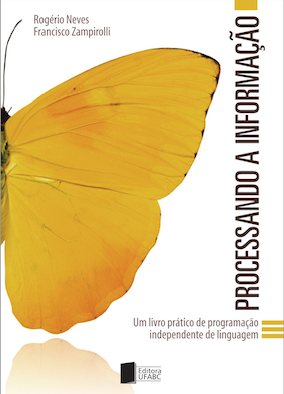
\includegraphics{"figs/Capa_Processando_Informacao.jpg"}

Este caderno (Notebook) é parte complementar \emph{online} do livro
\textbf{\href{https://editora.ufabc.edu.br/matematica-e-ciencias-da-computacao/58-processando-a-informacao}{Processando
a Informação}: um livro prático de programação independente de
linguagem}, que deve ser consultado no caso de dúvidas sobre os temas
apresentados.

\begin{quote}
Este conteúdo pode ser copiado e alterado livremente e foi inspirado
nesse livro.
\end{quote}

    \hypertarget{exercuxedcios}{%
\subsubsection{Exercícios}\label{exercuxedcios}}

    \begin{center}\rule{0.5\linewidth}{0.5pt}\end{center}

\begin{enumerate}
\def\labelenumi{\arabic{enumi}.}
\tightlist
\item
  Criar um vetor de entrada com \texttt{n} posições com valores inteiros
  positivos e como saída criar um outro vetor também com \texttt{n}
  posições, onde a cada posição \texttt{i} seja atribuído a cálculo do
  mínimo do seu vizinho de \texttt{v1} à esquerda \texttt{i-1}, do
  próprio elemento \texttt{i} e do seu vizinho à direita \texttt{i+1}.
\end{enumerate}

    \begin{center}\rule{0.5\linewidth}{0.5pt}\end{center}

\begin{enumerate}
\def\labelenumi{\arabic{enumi}.}
\setcounter{enumi}{1}
\tightlist
\item
  Criar um vetor com \texttt{n} posições com valores inteiros positivos
  e, como saída, criar um outro vetor também com \texttt{n} posições,
  onde em cada posição \texttt{i} seja atribuído a cálculo dos mínimos
  dos seus vizinhos de \texttt{v1} à esquerda \texttt{i-2} e
  \texttt{i-1}, do próprio elemento \texttt{i} e dos seus vizinhos à
  direita \texttt{i+1} e \texttt{i+2}. Generalize este código para os
  \texttt{m} vizinhos à esquerda e à direita.
\end{enumerate}

    \begin{center}\rule{0.5\linewidth}{0.5pt}\end{center}

\begin{enumerate}
\def\labelenumi{\arabic{enumi}.}
\setcounter{enumi}{2}
\tightlist
\item
  O MMC (Mínimo Múltiplo Comum) de dois ou mais números inteiros é o
  menor múltiplo inteiro positivo comum a todos eles. Fazer uma função
  chamada MMC que recebe um vetor de números inteiros e retorna o MMC de
  todos. Veja um exemplo abaixo para calcular o MMC de 12 e 15:
\end{enumerate}

    \begin{longtable}[]{@{}lll@{}}
\toprule
a & b & /\tabularnewline
\midrule
\endhead
12 & 15 & 2\tabularnewline
6 & 15 & 2\tabularnewline
3 & 15 & 3\tabularnewline
1 & 5 & 5\tabularnewline
1 & 1 & 60\tabularnewline
\bottomrule
\end{longtable}

\[MMC = 60 = 2*2*3*5\]

    \begin{center}\rule{0.5\linewidth}{0.5pt}\end{center}

\begin{enumerate}
\def\labelenumi{\arabic{enumi}.}
\setcounter{enumi}{3}
\tightlist
\item
  Criar um vetor de inteiros com n elementos. Inverter este vetor sem
  usar vetor auxiliar.
\end{enumerate}

    \begin{center}\rule{0.5\linewidth}{0.5pt}\end{center}

\begin{enumerate}
\def\labelenumi{\arabic{enumi}.}
\setcounter{enumi}{4}
\tightlist
\item
  Criar dois vetores de inteiros com n elementos cada. Calcular o
  produto escalar entre eles.
\end{enumerate}

    \hypertarget{processando-a-informauxe7uxe3o-cap.-5-vetores---pruxe1tica-3}{%
\subsection{Processando a Informação: Cap. 5: Vetores - Prática
3}\label{processando-a-informauxe7uxe3o-cap.-5-vetores---pruxe1tica-3}}

    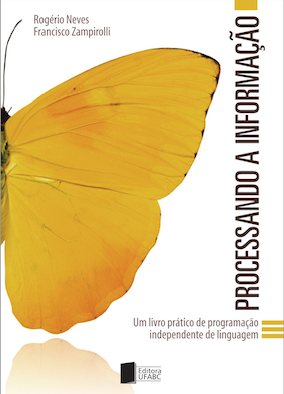
\includegraphics{"figs/Capa_Processando_Informacao.jpg"}

Este caderno (Notebook) é parte complementar \emph{online} do livro
\textbf{\href{https://editora.ufabc.edu.br/matematica-e-ciencias-da-computacao/58-processando-a-informacao}{Processando
a Informação}: um livro prático de programação independente de
linguagem}, que deve ser consultado no caso de dúvidas sobre os temas
apresentados.

\begin{quote}
Este conteúdo pode ser copiado e alterado livremente e foi inspirado
nesse livro.
\end{quote}

    \hypertarget{exercuxedcios}{%
\subsubsection{Exercícios}\label{exercuxedcios}}

Fontes:
\href{http://www.deinf.ufma.br/~csalles/prog/prog_lista2.pdf}{ref1},
\href{http://www.sistemas24horas.com.br/aulas/files_dic1/lista-exercicios-vetores-1.pdf}{ref2},
\href{https://fit.faccat.br/~fpereira/apostilas/exerc_resp_alg_mar2007.pdf}{ref3},
\href{https://docplayer.com.br/54457072-Laboratorio-de-programacao-a-exercicios-sobre-vetores-e-matrizes.html}{ref4},
\href{https://docplayer.com.br/21195395-Exercicios-vetores-e-matrizes.html}{ref5}

    \begin{center}\rule{0.5\linewidth}{0.5pt}\end{center}

\begin{enumerate}
\def\labelenumi{\arabic{enumi}.}
\tightlist
\item
  Dado um vetor qualquer com \(n\) números inteiros entre 0 e 9, faça um
  módulo que retorna o número que mais se repete.
\end{enumerate}

    \begin{center}\rule{0.5\linewidth}{0.5pt}\end{center}

\begin{enumerate}
\def\labelenumi{\arabic{enumi}.}
\setcounter{enumi}{1}
\tightlist
\item
  Escreva um módulo que retira todos os números repetidos das primeiras
  N posições de um vetor em ordem crescente, colocando-os em ordem
  crescente no final do vetor. Exemplo: Para o vetor \{1,2,2,3,3,4\}, a
  solução é \{1,2,3,4,2,3\}.
\end{enumerate}

    \begin{center}\rule{0.5\linewidth}{0.5pt}\end{center}

\begin{enumerate}
\def\labelenumi{\arabic{enumi}.}
\setcounter{enumi}{2}
\tightlist
\item
  Escreva um módulo que recebe um vetor lógico de 10 posições e oferece
  como resultado o produto da operação (((vet{[}0{]} E vet{[}1{]}) OU
  vet{[}2{]}) E vet{[}3{]}) \ldots{} e assim por diante.
\end{enumerate}

    \begin{center}\rule{0.5\linewidth}{0.5pt}\end{center}

\begin{enumerate}
\def\labelenumi{\arabic{enumi}.}
\setcounter{enumi}{3}
\tightlist
\item
  Faça um programa que leia 30 valores do tipo inteiro e armazene-os em
  um vetor. A seguir, o programa deverá informar (1) todos os números
  pares que existem no vetor; (2) o menor e o maior valor existente no
  vetor; (3) quantos dos valores do vetor são maiores que a média desses
  valores.
\end{enumerate}

    \begin{center}\rule{0.5\linewidth}{0.5pt}\end{center}

\begin{enumerate}
\def\labelenumi{\arabic{enumi}.}
\setcounter{enumi}{4}
\tightlist
\item
  Escreva um algoritmo que permita a leitura dos nomes de 10 pessoas e
  armaze os nomes lidos em um vetor. Após isto, o algoritmo deve
  permitir a leitura de mais 1 nome qualquer de pessoa e depois escrever
  a mensagem ACHEI, se o nome estiver entre os 10 nomes lidos
  anteriormente (guardados no vetor), ou NÃO ACHEI caso contrário.
\end{enumerate}

    \begin{center}\rule{0.5\linewidth}{0.5pt}\end{center}

\begin{enumerate}
\def\labelenumi{\arabic{enumi}.}
\setcounter{enumi}{5}
\tightlist
\item
  Escreva um algoritmo que permita a leitura das notas de uma turma de
  20 alunos. Calcular a média da turma e contar quantos alunos obtiveram
  nota acima desta média calculada. Escrever a média da turma e o
  resultado da contagem.
\end{enumerate}

    \begin{center}\rule{0.5\linewidth}{0.5pt}\end{center}

\begin{enumerate}
\def\labelenumi{\arabic{enumi}.}
\setcounter{enumi}{6}
\tightlist
\item
  Ler um vetor Q de 20 posições (aceitar somente números positivos).
  Escrever a seguir o valor do maior (e menor) elemento de Q e a
  respectiva posição que ele ocupa no vetor.
\end{enumerate}

    \begin{center}\rule{0.5\linewidth}{0.5pt}\end{center}

\begin{enumerate}
\def\labelenumi{\arabic{enumi}.}
\setcounter{enumi}{7}
\tightlist
\item
  Faça um algoritmo para ler um valor N qualquer (que será o tamanho dos
  vetores). Após, ler dois vetores A e B (de tamanho N cada um) e depois
  armazenar em um terceiro vetor Soma a soma dos elementos do vetor A
  com os do vetor B (respeitando as mesmas posições) e escrever o vetor
  Soma.
\end{enumerate}

    \begin{center}\rule{0.5\linewidth}{0.5pt}\end{center}

\begin{enumerate}
\def\labelenumi{\arabic{enumi}.}
\setcounter{enumi}{8}
\tightlist
\item
  Faça um algoritmo para ler e armazenar em um vetor a temperatura média
  de todos os dias do ano. Calcular e escrever:
\end{enumerate}

\begin{itemize}
\tightlist
\item
  Menor temperatura do ano
\item
  Maior temperatura do ano
\item
  Temperatura média anual
\item
  O número de dias no ano em que a temperatura foi inferior a média
  anual
\end{itemize}

    \begin{center}\rule{0.5\linewidth}{0.5pt}\end{center}

\begin{enumerate}
\def\labelenumi{\arabic{enumi}.}
\setcounter{enumi}{9}
\tightlist
\item
  Faça um algoritmo para ler 10 números e armazenar em um vetor. Após
  isto, o algoritmo deve ordenar os números no vetor em ordem crescente.
  Depois de ordenar os elementos do vetor em ordem crescente, deve ser
  lido mais um número qualquer e inserir esse novo número na posição
  correta, ou seja, mantendo a ordem crescente do vetor.
\end{enumerate}

    \begin{center}\rule{0.5\linewidth}{0.5pt}\end{center}

\begin{enumerate}
\def\labelenumi{\arabic{enumi}.}
\setcounter{enumi}{10}
\tightlist
\item
  Faça um algoritmo para ler um vetor de 20 números. Após isto, deverá
  ser lido mais um número qualquer e verificar se esse número existe no
  vetor ou não. Se existir, o algoritmo deve gerar um novo vetor sem
  esse número. (Considere que não haverão números repetidos no vetor).
\end{enumerate}

    \begin{center}\rule{0.5\linewidth}{0.5pt}\end{center}

\begin{enumerate}
\def\labelenumi{\arabic{enumi}.}
\setcounter{enumi}{11}
\tightlist
\item
  Faça um algoritmo para ler dois vetores V1 e V2 de 15 números cada.
  Calcular e escrever a quantidade de vezes que V1 e V2 possuem os
  mesmos números e nas mesmas posições (também, alterar para não ter
  essa última restrição).
\end{enumerate}

    \begin{center}\rule{0.5\linewidth}{0.5pt}\end{center}

\begin{enumerate}
\def\labelenumi{\arabic{enumi}.}
\setcounter{enumi}{12}
\tightlist
\item
  Faça um programa que leia 2 vetores com 10 elementos cada.
  Considerando cada vetor como sendo um conjunto, crie um terceiro
  vetor, que seja a união dos dois primeiros, e um quarto, que seja a
  intersecção entre os dois primeiros.
\end{enumerate}

    \begin{center}\rule{0.5\linewidth}{0.5pt}\end{center}

\begin{enumerate}
\def\labelenumi{\arabic{enumi}.}
\setcounter{enumi}{13}
\tightlist
\item
  Dado um vetor com números ordenados de forma não decrescente, faça uma
  função que imprime somente os números que não sejam repetidos.
\end{enumerate}

    \begin{center}\rule{0.5\linewidth}{0.5pt}\end{center}

\begin{enumerate}
\def\labelenumi{\arabic{enumi}.}
\setcounter{enumi}{14}
\tightlist
\item
  Faça uma função que recebe dois vetores de inteiros, com qualquer
  número de elementos cada. Ela deve imprimir todos os valores presentes
  nos dois vetores. Ex: se v1=\{19, 5, 2, 6\} e v2=\{5, 0, 9, 4, 18,
  56\} deverá ser impresso somente o valor 5.
\end{enumerate}

    \begin{center}\rule{0.5\linewidth}{0.5pt}\end{center}

\begin{enumerate}
\def\labelenumi{\arabic{enumi}.}
\setcounter{enumi}{15}
\tightlist
\item
  Faça um programa que dado o vetor unidimensional {[}2; 4; 35; 50; 23;
  17; 9; 12; 27; 5{]} retorne:\\
\end{enumerate}

\begin{itemize}
\tightlist
\item
  maior valor
\item
  média dos valores
\item
  os valores dispostos em ordem crescente
\item
  sub conjunto de valores primos que está contido no vetor
\end{itemize}

    \begin{center}\rule{0.5\linewidth}{0.5pt}\end{center}

\begin{enumerate}
\def\labelenumi{\arabic{enumi}.}
\setcounter{enumi}{16}
\tightlist
\item
  Faça um programa que:
\end{enumerate}

\begin{itemize}
\tightlist
\item
  leia 7 valores inteiros e os armazene em um vetor. Listar o vetor com
  as referidasposições de armazenamento de cada valor.
\item
  ofereça uma função de pesquisa onde dado um valor inteiro qualquer de
  entrada retornar a posição deste valor dentro do vetor, e caso este
  valor não esteja presente no vetor retornar --1.
\item
  ofereça uma função que troque os valores contido no vetor pela
  seguinte política: cada elemento i dentro do vetor será substituído
  pela soma de todos os (i-1) elementos mais o elemento i. Por exemplo,
  dado um vetor {[}1; 2; 3; 4; 5{]} após a aplicação da função teríamos
  esse vetor preenchido com os seguintes valores {[}1;3; 6; 10; 15{]}.
\end{itemize}

    \begin{center}\rule{0.5\linewidth}{0.5pt}\end{center}

\begin{enumerate}
\def\labelenumi{\arabic{enumi}.}
\setcounter{enumi}{17}
\tightlist
\item
  Escrever um programa para ler um vetor de 25 elementos do tipo inteiro
  e que, apósos valores serem lidos, verifique se existem números
  repetidos dentro do vetor. Caso exista, deverão ser informados quais
  são estes números e quantas vezes eles foram repetidos.
\end{enumerate}

    \begin{center}\rule{0.5\linewidth}{0.5pt}\end{center}

\begin{enumerate}
\def\labelenumi{\arabic{enumi}.}
\setcounter{enumi}{18}
\tightlist
\item
  Escreva um programa em C para ler um vetor de 10 elementos inteiros.
  Excluir o1 o elemento do vetor deslocando os elementos subsequentes de
  uma posição parao inicio. Imprimir o vetor após a retirada do primeiro
  elemento.
\end{enumerate}

    \begin{center}\rule{0.5\linewidth}{0.5pt}\end{center}

\begin{enumerate}
\def\labelenumi{\arabic{enumi}.}
\setcounter{enumi}{19}
\tightlist
\item
  Escreva um programa em C para ler um vetor X de 10 elementos e um
  valor P(aceitar apenas valores entre 0 e 9) que representa a posição
  de um elemento dentrodo vetor X. Imprimir o valor do elemento que
  ocupa a posição informada. Logo após excluir esse elemento do vetor
  fazendo com que os elementos subseqüentes (sehouverem) sejam
  deslocados de 1 posição para o inicio. Imprimir o vetor X após a
  exclusão ter sido executada.
\end{enumerate}

    \begin{center}\rule{0.5\linewidth}{0.5pt}\end{center}

\begin{enumerate}
\def\labelenumi{\arabic{enumi}.}
\setcounter{enumi}{20}
\tightlist
\item
  Faça um programa que receba uma lista com nomes de alunos, as notas de
  cada aluno e a nota mínima para aprovação na disciplina. O aluno é
  considerado aprovadose a média de suas notas forma maior ou igual a
  nota mínima para aprovação. O programa deve informar uma lista de
  alunos aprovados e outra de alunos reprovados.
\end{enumerate}

    \begin{center}\rule{0.5\linewidth}{0.5pt}\end{center}

\begin{enumerate}
\def\labelenumi{\arabic{enumi}.}
\setcounter{enumi}{21}
\tightlist
\item
  Escreva um programa para ler \(n\) palavras. A seguir imprimir as
  palavras em ordem alfabética.
\end{enumerate}

    \begin{center}\rule{0.5\linewidth}{0.5pt}\end{center}

\begin{enumerate}
\def\labelenumi{\arabic{enumi}.}
\setcounter{enumi}{22}
\tightlist
\item
  Escreva um programa para ler uma frase e contar o número de
  ocorrências de cada uma das 15 primeiras letras do alfabeto. Imprimir
  as contagens.
\end{enumerate}

    \begin{center}\rule{0.5\linewidth}{0.5pt}\end{center}

\begin{enumerate}
\def\labelenumi{\arabic{enumi}.}
\setcounter{enumi}{23}
\tightlist
\item
  Escreva um programa para ler uma frase e uma letra. A seguir retirar
  da frase, todas as letras iguais a informada. Imprimir a frase
  modificada.
\end{enumerate}

    \begin{center}\rule{0.5\linewidth}{0.5pt}\end{center}

\begin{enumerate}
\def\labelenumi{\arabic{enumi}.}
\setcounter{enumi}{24}
\tightlist
\item
  Escreva um programa para ler uma frase e contar o número de palavras
  existentes na frase. Considere palavra um conjunto qualquer de
  caracteres separados por um conjunto qualquer de espaços em branco.
\end{enumerate}

    \begin{center}\rule{0.5\linewidth}{0.5pt}\end{center}

\begin{enumerate}
\def\labelenumi{\arabic{enumi}.}
\setcounter{enumi}{25}
\tightlist
\item
  Escreva um programa que leia n números inteiros no intervalo
  {[}0,50{]} e os armazeneem um vetor estaticamente alocado com 100
  posições. Preencha um segundo vetor, também alocado estaticamente,
  apenas com os números ímpares do primeiro vetor. Imprima os dois
  vetores, 10 elementos por linha.
\end{enumerate}

    \begin{center}\rule{0.5\linewidth}{0.5pt}\end{center}

\begin{enumerate}
\def\labelenumi{\arabic{enumi}.}
\setcounter{enumi}{26}
\tightlist
\item
  Leia 10 números inteiros e armazene em um vetor v. Crie dois novos
  vetores v1 e v2. Copie os valores ímpares de v para v1, e os valores
  pares de v para v2. Note que cada um dos vetores v1 e v2 têm no máximo
  10 elementos, mas nem todos os elementos são utilizados. No final
  escreva os elementos UTILIZADOS de v1 e v2.
\end{enumerate}

    \begin{center}\rule{0.5\linewidth}{0.5pt}\end{center}

\begin{enumerate}
\def\labelenumi{\arabic{enumi}.}
\setcounter{enumi}{27}
\tightlist
\item
  Faça um programa para ler 10 números DIFERENTES a serem armazenados em
  um vetor. Os dados deverão ser armazenados no vetor na ordem que forem
  sendo lidos, sendo que caso o usuário digite um número que já foi
  digitado anteriormente, o programadeverá pedir para ele digitar outro
  número. Note que cada valor digitado pelo usuário deve ser pesquisado
  no vetor, verificando se ele existe entre os números que já foram
  fornecidos. Exibir na tela o vetor final que foi digitado.
\end{enumerate}

    \begin{center}\rule{0.5\linewidth}{0.5pt}\end{center}

\begin{enumerate}
\def\labelenumi{\arabic{enumi}.}
\setcounter{enumi}{28}
\tightlist
\item
  Faça um programa que leia dez conjuntos de dois valores, o primeiro
  representando o número do aluno e o segundo representando a sua altura
  em metros. Encontre o aluno mais baixo e o mais alto. Mostre o número
  do aluno mais baixo e do mais alto, juntamente com suas alturas.
\end{enumerate}

    \begin{center}\rule{0.5\linewidth}{0.5pt}\end{center}

\begin{enumerate}
\def\labelenumi{\arabic{enumi}.}
\setcounter{enumi}{29}
\tightlist
\item
  Faça um programa que leia dois números a e b (positivos menores que
  10000) e:Crie um vetor onde cada posição é um algarismo do número. A
  primeira posição é o algarismo menos significativo;Crie um vetor que
  seja a soma de a e b, mas faça-o usando apenas os vetores construídos
  anteriormente. Dica: some as posições correspondentes. Se a soma
  ultrapassar 10, subtraia 10 do resultado e some 1 à próxima posição.
\end{enumerate}

    \begin{center}\rule{0.5\linewidth}{0.5pt}\end{center}

\begin{enumerate}
\def\labelenumi{\arabic{enumi}.}
\setcounter{enumi}{30}
\tightlist
\item
  Faça um programa que leia dois números n e m e:Crie e leia um vetor
  de inteiros de n posições;Crie e leia um vetor de inteiros de m
  posições;Crie e construa um vetor de inteiros que seja a interseção
  entre os dois vetores anteriores, ou seja, que contém apenas os
  números que estão em ambos os vetores.Crie e construa um quarto vetor
  de inteiros que seja a uniãoo entre os dois vetores anteriores lidos,
  ou seja, que contém os elementos dos dois vetores.
\end{enumerate}

    \begin{center}\rule{0.5\linewidth}{0.5pt}\end{center}

\begin{enumerate}
\def\labelenumi{\arabic{enumi}.}
\setcounter{enumi}{31}
\tightlist
\item
  Faça um programa que receba o nome de \(n\) clientes e armazene-os em
  um vetor. Em um segundo vetor, armazene a quantidade de DVDs locados
  em 2009 por cada um dos clientes. Sabe-se que, para cada dez locações,
  o cliente tem direito a uma locação grátis. Faça um programa que
  mostre o nome de todos os clientes, com a quantidade de locações
  grátis a que ele tem direito.
\end{enumerate}

    \begin{center}\rule{0.5\linewidth}{0.5pt}\end{center}

\begin{enumerate}
\def\labelenumi{\arabic{enumi}.}
\setcounter{enumi}{32}
\tightlist
\item
  Faça um programa que preencha três vetores com \(n\) posições cada um:
  o primeiro vetor, com os nomes dos produtos; o segundo vetor, com os
  códigos dos produtos; e o terceiro vetor; com os preços dos produtos.
  Mostre um relatório apenas com o nome, o código, o preço e o novo
  preço dos produtos que sofrerão aumento. Sabe-se que os produtos que
  sofrerão aumento são aqueles que possuem código par ou preço superiora
  R\$ 1.000,00. Sabe-se ainda que, para os produtos que satisfizerem às
  duas condições anteriores, código e preço, o aumento será de 20\%;
  para aqueles que satisfazerem apenas a condição de código, o aumento
  será de 15\%; e aqueles que satisfazerem apenas a condição de preço, o
  aumento será de 10\%.
\end{enumerate}

    \begin{center}\rule{0.5\linewidth}{0.5pt}\end{center}

\begin{enumerate}
\def\labelenumi{\arabic{enumi}.}
\setcounter{enumi}{33}
\tightlist
\item
  Faça um vetor de tamanho 50 preenchido com o seguinte valor:
  \((i+5i)\%i\), sendo \(i\) aposição do elemento no vetor, em seguida
  imprima o vetor na tela.
\end{enumerate}

    \begin{center}\rule{0.5\linewidth}{0.5pt}\end{center}

\begin{enumerate}
\def\labelenumi{\arabic{enumi}.}
\setcounter{enumi}{34}
\tightlist
\item
  Faça um programa que calcule o desvio padrão (STD) de um vetor \(v\)
  contendo \(n\) números, ondem \(m\) a média do vetor.
\end{enumerate}

\[ STD = \sqrt{\frac{1}{n-1} \sum_{i=0}^{n-1}(v[i]-m)^2} \]

    \hypertarget{processando-a-informauxe7uxe3o-cap.-6-matrizes}{%
\section{Processando a Informação: Cap. 6:
Matrizes}\label{processando-a-informauxe7uxe3o-cap.-6-matrizes}}

    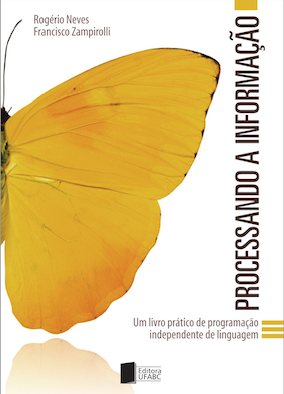
\includegraphics{"figs/Capa_Processando_Informacao.jpg"}

Este caderno (Notebook) é parte complementar \emph{online} do livro
\textbf{\href{https://editora.ufabc.edu.br/matematica-e-ciencias-da-computacao/58-processando-a-informacao}{Processando
a Informação}: um livro prático de programação independente de
linguagem}, que deve ser consultado no caso de dúvidas sobre os temas
apresentados.

\begin{quote}
Este conteúdo pode ser copiado e alterado livremente e foi inspirado
nesse livro.
\end{quote}

    \hypertarget{sumuxe1rio}{%
\subsection{Sumário}\label{sumuxe1rio}}

\begin{itemize}
\tightlist
\item
  Revisão do capítulo anterior
\item
  Introdução
\item
  Instanciando matrizes
\item
  Acessando elementos de uma matriz
\item
  Formas de percorrer uma matriz
\item
  Aplicações usando matrizes
\item
  Revisão deste capítulo
\item
  Exercícios
\end{itemize}

    \hypertarget{revisuxe3o-do-capuxedtulo-anterior-vetores}{%
\subsection{Revisão do capítulo anterior
(Vetores)}\label{revisuxe3o-do-capuxedtulo-anterior-vetores}}

    \begin{itemize}
\item
  Introdução \textgreater{} Vetores são estruturas para armazenar vários
  elementos de um mesmo tipo de dados em uma única variável.
\item
  Trabalhando com vetores \textgreater{} Cada linguagem possui uma
  sintaxe própria para declarar e alocar vetores.
\item
  Acessando elementos de um vetor \textgreater{} \textbf{ATENÇÃO} para
  não acessar uma posição do vetor não reservada/alocada, geralmente
  \texttt{\textless{}0} e \texttt{\textgreater{}=n}.
\item
  Formas de percorrer um vetor \textgreater{} É possível varrer um vetor
  na forma \textbf{\emph{raster}} e \textbf{\emph{anti-raster}}, também
  usando diferentes passos, mas geralmente é passo=1.
\item
  Modularização e vetores \textgreater{} Muito útil usar principalmente
  os módulos de \texttt{leiaVetor} e \texttt{escrevaVetor}, podendo ser
  reaproveitados em vários códigos.
\item
  Tudo que foi visto no capítulo anterior de \textbf{Vetores} (ou
  estruturas \textbf{unidimensional} ou \textbf{1D}) se estende a
  estrutura de \textbf{Matrizes} (ou estruturas \textbf{bidimensional}
  ou \textbf{2D)}).
\end{itemize}

    \hypertarget{introduuxe7uxe3o}{%
\subsection{Introdução}\label{introduuxe7uxe3o}}

    \begin{itemize}
\item
  Existem situações onde é necessário estender a definição de vetor para
  mais de uma dimensão de dados.
\item
  Por exemplo, uma forma muito utilizada de manipulação de dados é em
  tabelas.
\item
  Como exemplo, para listar todos os alunos de uma turma e suas notas em
  uma disciplina,

  \begin{itemize}
  \tightlist
  \item
    as linhas da tabela podem armazenar a identificação dos alunos na
    primeira coluna,
  \item
    nas colunas seguintes podem armazenar as notas da prova1, prova2,
    projeto e, numa última coluna, podem armazenar a nota final do
    aluno.
  \end{itemize}
\item
  Analogamente a um vetor, em uma matriz cada elemento possui apenas um
  dado.
\item
  Além disso, na maioria das linguagens de programação, todos os
  elementos de uma matriz são de um mesmo tipo de dado.
\end{itemize}

    \begin{itemize}
\item
  Um outro exemplo de matrizes muito usado, especialmente com a
  popularização dos dispositivos móveis como celulares e \emph{tablets},
  que comumente trazem câmeras digitais acopladas, ocorre no
  armazenamento e processamento digital de imagens.
\item
  Mas antes das câmeras digitais, já havia \emph{scanners} e
  digitalizadores, e uma imagem pode ser representada por uma
  \textbf{matriz} em um computador.
\item
  Veja o conteúdo no \textbf{\emph{QRCode}} (imagem=matriz) abaixo
  usando um aplicativo leitor de QRCode, disponível para
  \emph{Smartphones} (teste nesta imagem).
\item
  O conteúdo do \textbf{\emph{QRCode}} direciona para uma página
  \emph{web} mostrando uma imagem colorida.
\item
  As imagens coloridas podem ser armazenada em uma estrutura de matriz
  \textbf{tridimensional}, onde cada dimensão armazena uma matriz para
  uma cor primária (RGB - \emph{Red-Green-Blue} ou vermelhor, verde e
  azul).
\end{itemize}


\includegraphics{"figs/image38.png"}

    \begin{figure}
\centering
\caption{image.png}
\end{figure}

    \hypertarget{instanciando-matrizes}{%
\subsection{Instanciando Matrizes}\label{instanciando-matrizes}}

    \begin{itemize}
\item
  Nas linguagens MatLab e R, uma matriz é definida com elementos da
  posição \texttt{(1,1)} até a posição \texttt{(L,\ C)}, onde \texttt{L}
  representa o número de linhas e \texttt{C} representa o número de
  colunas de uma matriz.
\item
  Na maioria das linhagens de programação, no entanto, o índice começa
  no zero, sendo os elementos de uma matriz armazenados da posição
  \texttt{(0,0)} até \texttt{(L-1,C-1)}.
\item
  Nos exemplos a seguir são apresentados alguns exemplos de instanciação
  de matrizes em diferentes linguagens de programação.
\end{itemize}

    \hypertarget{acessando-elementos-de-uma-matriz}{%
\subsection{Acessando elementos de uma
matriz}\label{acessando-elementos-de-uma-matriz}}

    \begin{itemize}
\tightlist
\item
  Uma matriz está pronta para se inserir elementos ou se alterar seus
  dados após instanciada e alocada na memória, em todas as suas
  dimensões.
\item
  Veja uma forma de visualizar uma matriz 2D na Figura abaixo.
\end{itemize}

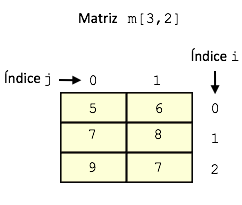
\includegraphics{"figs/image40.png"}

    \begin{figure}
\centering
\caption{image.png}
\end{figure}

    \begin{itemize}
\tightlist
\item
  Essa figura ilustra uma matriz com \texttt{3} linhas e \texttt{2}
  colunas.
\item
  Para visualizar seus elementos podemos usar os índices \texttt{i} e
  \texttt{j},

  \begin{itemize}
  \tightlist
  \item
    com valores para as linhas \texttt{0\textless{}=i\textless{}3} e
  \item
    para as colunas \texttt{0\textless{}=j\textless{}2}.
  \end{itemize}
\item
  Analogamente ao vetor, mas com uma dimensão a mais, a matriz recebe
  valores para os seus elementos, conforme a seguinte estrutura em
  pseudocódigo:
\end{itemize}

    \begin{verbatim}
Instanciar uma matriz m com 3 linhas e 2 colunas
m[0,0] = 5 # linha i=0
m[0,1] = 6
m[1,0] = 7 # linha i=1
m[1,1] = 8
m[2,0] = 9 # linha i=2
m[2,1] = 7
\end{verbatim}

    \hypertarget{formas-de-se-percorrer-uma-matriz}{%
\subsection{Formas de se percorrer uma
matriz}\label{formas-de-se-percorrer-uma-matriz}}

    \begin{itemize}
\tightlist
\item
  Analogamente ao vetor, uma matriz, após criada, possui tamanho fixo.
\item
  Geralmente, para cada dimensão da matriz, é recomendado usar uma
  estrutura de repetição \texttt{para}, \textgreater{} com o objetivo de
  tornar o código mais compacto e genérico para matrizes de quaisquer
  dimensões.
\item
  Além disso, é natural percorrer (ou varrer) a matriz

  \begin{itemize}
  \tightlist
  \item
    da linha \texttt{i=0} até a linha \texttt{i\textless{}L}, onde L
    representa o número de linhas de uma matriz.
  \item
    e da coluna \texttt{j=0} até a coluna \texttt{j\textless{}C}.
  \end{itemize}
\item
  No exemplo a seguir em pseudocódigo, uma matriz \texttt{m} é criada
  com \texttt{6} elementos, sendo três linhas e \texttt{2} colunas, e os
  dois laços \texttt{para} inicializam todos os seus elementos com o
  valor 0.
\end{itemize}

    \begin{verbatim}
Instanciar uma matriz m com 3 linhas e 2 colunas 
inteiros L=3, C=2
Para cada i, de i=0; até i<L; passo i=i+1 faça
    Para cada j, de j=0; até j<C; passo j=j+1 faça
        m[i,j] = 0
\end{verbatim}

    \begin{itemize}
\item
  Existem várias formas de percorrer (ou varrer) uma matriz usando uma
  estrutura de repetição.
\item
  Por exemplo, é possível percorrer uma matriz

  \begin{itemize}
  \tightlist
  \item
    do primeiro elemento \texttt{m{[}0,0{]}} \textgreater{}
    (convencionando como canto superior esquerdo)
  \item
    até o último elemento \texttt{m{[}L-1,C-1{]}} \textgreater{}
    (convencionando como canto inferior direito da matriz),
  \item
    linha por linha, ou coluna por coluna.
  \end{itemize}
\item
  Esse tipo de varredura é chamada \textbf{\emph{raster}}.
\item
  A varredura inversa é chamada \textbf{\emph{anti-raster}}, do último
  elemento inferior direito, até o primeiro elemento superior esquerdo.
\end{itemize}

    \hypertarget{exemplo-01---lerescrever-matriz}{%
\subsection{Exemplo 01 - Ler/Escrever
matriz}\label{exemplo-01---lerescrever-matriz}}

    \begin{itemize}
\item
  Analogamente ao que foi feito no capítulo anterior sobre vetores, onde
  alocamos os vetores em tempo de execução através de métodos, é
  possível usar modularização para melhorar a organização, manutenção e
  reaproveitamento de código.
\item
  Aqui é apresentado um método \texttt{leiaMatriz} e
  \texttt{escrevaMatriz} genéricos
\item
  Para entrada de dados, ou seja, inserir valores nos elementos alocados
  na memória para uma matriz.
\item
  Além de saída de dados, para escrever a matriz, linha por linha.
\end{itemize}

    \hypertarget{pseudocuxf3digo}{%
\paragraph{Pseudocódigo}\label{pseudocuxf3digo}}

    \textbf{Exemplo 01:} Considere um algoritmo para: * Ler um inteiro
\texttt{L} (linhas) representando o número de alunos, * Ler um inteiro
\texttt{C} representando o número de avaliações. * Considere a primeira
coluna o \texttt{RA} do aluno, assim \texttt{C=C+1}. * Criar uma matriz
\texttt{m} com dimensões \texttt{LxC}. * Ler todos os elementos da
matriz. * Escrever todos os elementos da matriz, formando a saída, linha
por linha, por exemplo, para uma matriz com \texttt{2} alunos e
\texttt{3} avaliações, escreva:

\begin{verbatim}
LISTA DE ALUNOS vs Avaliações:
1234 4 3 9
3456 6 4 8
\end{verbatim}

    \begin{verbatim}
Função inteiro m[][] leiaMatriz(inteiro L, inteiro C):
    Instanciar e alocar uma matriz m de Reais com L x C
    Para cada i, de i=0; até i<L; passo i=i+1 faça
        Para cada j, de j=0; até j<C; passo j=j+1 faça
            m[i,j] = leia("Digite um número inteiro:");

Função escrevaMatriz(inteiro m[][], inteiro L, inteiro C): 
    Instanciar e alocar uma matriz m de Reais com L x C
    Para cada i, de i=0; até i<L; passo i=i+1 faça
        Para cada j, de j=0; até j<C; passo j=j+1 faça
            escreva(" ", m[i,j]);
        escreva("\n"); // pula linha

// PROGRAMA PRINCIPAL
// ENTRADAS
inteiro L = leia("Digite o numero de alunos:")
inteiro C = leia("Digite o numero de avaliações:")
C = C + 1  // a primeira coluna é o RA
Instanciar uma matriz m com L linhas e C colunas 

m = leiaMatriz(L,C)
// PROCESSAMENTO: ?

// SAÍDA
escrevaMatriz(m)
\end{verbatim}

    \hypertarget{casos-para-teste-moodlevpl}{%
\paragraph{Casos para Teste
Moodle+VPL}\label{casos-para-teste-moodlevpl}}

Para o professor criar uma atividade VPL no Moodle para este Exemplo 01,
basta incluir em \texttt{Casos\ para\ teste}, o seguinte texto (pode
incluir mais casos):

\begin{verbatim}
case=caso1
input=2
3
1234 
4 
3 
9
3456
6
4
8
output=
LISTA DE ALUNOS vs Avaliações:
1234 4 3 9
3456 6 4 8
\end{verbatim}

    \begin{tcolorbox}[breakable, size=fbox, boxrule=1pt, pad at break*=1mm,colback=cellbackground, colframe=cellborder]
\prompt{In}{incolor}{1}{\boxspacing}
\begin{Verbatim}[commandchars=\\\{\}]
\PY{o}{\PYZpc{}\PYZpc{}writefile} cap6ex01.c
\PY{c+c1}{\PYZsh{}include \PYZlt{}stdio.h\PYZgt{}}
\PY{c+c1}{\PYZsh{}include\PYZlt{}malloc.h\PYZgt{}  }

\PY{n+nb}{int} \PY{o}{*}\PY{o}{*} \PY{n}{leiaMatriz}\PY{p}{(}\PY{n+nb}{int} \PY{n}{L}\PY{p}{,} \PY{n+nb}{int} \PY{n}{C}\PY{p}{)} \PY{p}{\PYZob{}}
  \PY{n+nb}{int} \PY{o}{*}\PY{o}{*}\PY{n}{m} \PY{o}{=} \PY{p}{(}\PY{n+nb}{int} \PY{o}{*}\PY{o}{*}\PY{p}{)}\PY{n}{malloc}\PY{p}{(}\PY{n}{L}\PY{o}{*}\PY{n}{sizeof}\PY{p}{(}\PY{n+nb}{int}\PY{o}{*}\PY{p}{)}\PY{p}{)}\PY{p}{;} 
  \PY{k}{for} \PY{p}{(}\PY{n+nb}{int} \PY{n}{i} \PY{o}{=} \PY{l+m+mi}{0}\PY{p}{;} \PY{n}{i} \PY{o}{\PYZlt{}} \PY{n}{L}\PY{p}{;} \PY{n}{i}\PY{o}{+}\PY{o}{+}\PY{p}{)} \PY{p}{\PYZob{}}
    \PY{n}{m}\PY{p}{[}\PY{n}{i}\PY{p}{]} \PY{o}{=} \PY{p}{(}\PY{n+nb}{int} \PY{o}{*}\PY{p}{)}\PY{n}{malloc}\PY{p}{(}\PY{n}{C} \PY{o}{*} \PY{n}{sizeof}\PY{p}{(}\PY{n+nb}{int}\PY{p}{)}\PY{p}{)}\PY{p}{;} \PY{o}{/}\PY{o}{/} \PY{k}{for} \PY{n}{each} \PY{n}{row} \PY{n}{allocate} \PY{n}{C} \PY{n}{ints}
    \PY{k}{for} \PY{p}{(}\PY{n+nb}{int} \PY{n}{j} \PY{o}{=} \PY{l+m+mi}{0}\PY{p}{;} \PY{n}{j} \PY{o}{\PYZlt{}} \PY{n}{C}\PY{p}{;} \PY{n}{j}\PY{o}{+}\PY{o}{+}\PY{p}{)} \PY{p}{\PYZob{}}
      \PY{n}{scanf}\PY{p}{(}\PY{l+s+s2}{\PYZdq{}}\PY{l+s+si}{\PYZpc{}d}\PY{l+s+s2}{\PYZdq{}}\PY{p}{,} \PY{o}{\PYZam{}}\PY{n}{m}\PY{p}{[}\PY{n}{i}\PY{p}{]}\PY{p}{[}\PY{n}{j}\PY{p}{]}\PY{p}{)}\PY{p}{;} 
    \PY{p}{\PYZcb{}}
  \PY{p}{\PYZcb{}}
  \PY{k}{return} \PY{n}{m}\PY{p}{;}
\PY{p}{\PYZcb{}}

\PY{o}{/}\PY{o}{/} \PY{n}{you} \PY{n}{must} \PY{n}{supply} \PY{n}{the} \PY{n}{number} \PY{n}{of} \PY{n}{rows}
\PY{n}{void} \PY{n}{free\PYZus{}matrix}\PY{p}{(}\PY{n+nb}{int} \PY{o}{*}\PY{o}{*}\PY{n}{m}\PY{p}{,} \PY{n+nb}{int} \PY{n}{L}\PY{p}{)} 
\PY{p}{\PYZob{}}
    \PY{o}{/}\PY{o}{/} \PY{n}{first} \PY{n}{free} \PY{n}{each} \PY{n}{row}
    \PY{k}{for} \PY{p}{(}\PY{n+nb}{int} \PY{n}{i} \PY{o}{=} \PY{l+m+mi}{0}\PY{p}{;} \PY{n}{i} \PY{o}{\PYZlt{}} \PY{n}{L}\PY{p}{;} \PY{n}{i}\PY{o}{+}\PY{o}{+}\PY{p}{)} \PY{p}{\PYZob{}}
         \PY{n}{free}\PY{p}{(}\PY{n}{m}\PY{p}{[}\PY{n}{i}\PY{p}{]}\PY{p}{)}\PY{p}{;}
    \PY{p}{\PYZcb{}}

    \PY{o}{/}\PY{o}{/} \PY{n}{Eventually} \PY{n}{free} \PY{n}{the} \PY{n}{memory} \PY{n}{of} \PY{n}{the} \PY{n}{pointers} \PY{n}{to} \PY{n}{the} \PY{n}{rows}
    \PY{n}{free}\PY{p}{(}\PY{n}{m}\PY{p}{)}\PY{p}{;}
 \PY{p}{\PYZcb{}}

\PY{n}{void} \PY{n}{escrevaMatriz}\PY{p}{(}\PY{n+nb}{int} \PY{o}{*}\PY{o}{*}\PY{n}{m}\PY{p}{,} \PY{n+nb}{int} \PY{n}{L}\PY{p}{,} \PY{n+nb}{int} \PY{n}{C}\PY{p}{)} \PY{p}{\PYZob{}}
  \PY{k}{for} \PY{p}{(}\PY{n+nb}{int} \PY{n}{i} \PY{o}{=} \PY{l+m+mi}{0}\PY{p}{;} \PY{n}{i} \PY{o}{\PYZlt{}} \PY{n}{L}\PY{p}{;} \PY{n}{i}\PY{o}{+}\PY{o}{+}\PY{p}{)} \PY{p}{\PYZob{}}
   \PY{k}{for} \PY{p}{(}\PY{n+nb}{int} \PY{n}{j} \PY{o}{=} \PY{l+m+mi}{0}\PY{p}{;} \PY{n}{j} \PY{o}{\PYZlt{}} \PY{n}{C}\PY{p}{;} \PY{n}{j}\PY{o}{+}\PY{o}{+}\PY{p}{)} \PY{p}{\PYZob{}}
      \PY{n}{printf}\PY{p}{(}\PY{l+s+s2}{\PYZdq{}}\PY{l+s+si}{\PYZpc{}d}\PY{l+s+se}{\PYZbs{}t}\PY{l+s+s2}{\PYZdq{}}\PY{p}{,} \PY{n}{m}\PY{p}{[}\PY{n}{i}\PY{p}{]}\PY{p}{[}\PY{n}{j}\PY{p}{]}\PY{p}{)}\PY{p}{;} 
   \PY{p}{\PYZcb{}}
   \PY{n}{printf}\PY{p}{(}\PY{l+s+s2}{\PYZdq{}}\PY{l+s+se}{\PYZbs{}n}\PY{l+s+s2}{\PYZdq{}}\PY{p}{)}\PY{p}{;}
  \PY{p}{\PYZcb{}}
\PY{p}{\PYZcb{}}
\PY{n+nb}{int} \PY{n}{main}\PY{p}{(}\PY{n}{void}\PY{p}{)} \PY{p}{\PYZob{}}
  \PY{o}{/}\PY{o}{/} \PY{n}{ENTRADA} \PY{n}{DE} \PY{n}{DADOS}
  \PY{n+nb}{int} \PY{n}{L}\PY{p}{,} \PY{n}{C}\PY{p}{,} \PY{o}{*}\PY{o}{*}\PY{n}{m}\PY{p}{;}   \PY{o}{/}\PY{o}{/} \PY{n}{variaveis} \PY{n}{de} \PY{n}{referência} \PY{n}{m}
  \PY{n}{printf}\PY{p}{(}\PY{l+s+s2}{\PYZdq{}}\PY{l+s+s2}{Digite o número de alunos: }\PY{l+s+s2}{\PYZdq{}}\PY{p}{)}\PY{p}{;}
  \PY{n}{scanf}\PY{p}{(}\PY{l+s+s2}{\PYZdq{}}\PY{l+s+si}{\PYZpc{}d}\PY{l+s+s2}{\PYZdq{}}\PY{p}{,} \PY{o}{\PYZam{}}\PY{n}{L}\PY{p}{)}\PY{p}{;}

  \PY{n}{printf}\PY{p}{(}\PY{l+s+s2}{\PYZdq{}}\PY{l+s+s2}{Digite o número de avaliações: }\PY{l+s+s2}{\PYZdq{}}\PY{p}{)}\PY{p}{;}
  \PY{n}{scanf}\PY{p}{(}\PY{l+s+s2}{\PYZdq{}}\PY{l+s+si}{\PYZpc{}d}\PY{l+s+s2}{\PYZdq{}}\PY{p}{,} \PY{o}{\PYZam{}}\PY{n}{C}\PY{p}{)}\PY{p}{;}

  \PY{n}{C} \PY{o}{=} \PY{n}{C} \PY{o}{+} \PY{l+m+mi}{1}\PY{p}{;} \PY{o}{/}\PY{o}{/} \PY{n}{a} \PY{n}{primeira} \PY{n}{coluna} \PY{n}{é} \PY{n}{o} \PY{n}{RA} \PY{n}{do} \PY{n}{aluno}

  \PY{n}{printf}\PY{p}{(}\PY{l+s+s2}{\PYZdq{}}\PY{l+s+s2}{Digite os elementos da matriz}\PY{l+s+s2}{\PYZdq{}}\PY{p}{)}\PY{p}{;}
  \PY{n}{m} \PY{o}{=} \PY{n}{leiaMatriz}\PY{p}{(}\PY{n}{L}\PY{p}{,}\PY{n}{C}\PY{p}{)}\PY{p}{;}

  \PY{o}{/}\PY{o}{/} \PY{n}{PROCESSAMENTO} \PY{err}{?}

  \PY{o}{/}\PY{o}{/} \PY{n}{SAÍDA} \PY{n}{DE} \PY{n}{DADOS}
  \PY{n}{printf}\PY{p}{(}\PY{l+s+s2}{\PYZdq{}}\PY{l+s+se}{\PYZbs{}n}\PY{l+s+s2}{LISTA DE ALUNOS vs Avaliações:}\PY{l+s+se}{\PYZbs{}n}\PY{l+s+s2}{\PYZdq{}}\PY{p}{)}\PY{p}{;}
  \PY{n}{printf}\PY{p}{(}\PY{l+s+s2}{\PYZdq{}}\PY{l+s+s2}{RA }\PY{l+s+s2}{\PYZdq{}}\PY{p}{)}\PY{p}{;}
  \PY{k}{for} \PY{p}{(}\PY{n+nb}{int} \PY{n}{i} \PY{o}{=} \PY{l+m+mi}{0}\PY{p}{;} \PY{n}{i} \PY{o}{\PYZlt{}} \PY{n}{C}\PY{o}{\PYZhy{}}\PY{l+m+mi}{1}\PY{p}{;} \PY{n}{i}\PY{o}{+}\PY{o}{+}\PY{p}{)} \PY{p}{\PYZob{}}
    \PY{n}{printf}\PY{p}{(}\PY{l+s+s2}{\PYZdq{}}\PY{l+s+se}{\PYZbs{}t}\PY{l+s+si}{\PYZpc{}d}\PY{l+s+s2}{\PYZdq{}}\PY{p}{,}\PY{p}{(}\PY{n}{i}\PY{o}{+}\PY{l+m+mi}{1}\PY{p}{)}\PY{p}{)}\PY{p}{;} 
  \PY{p}{\PYZcb{}}
  \PY{n}{printf}\PY{p}{(}\PY{l+s+s2}{\PYZdq{}}\PY{l+s+se}{\PYZbs{}n}\PY{l+s+s2}{\PYZdq{}}\PY{p}{)}\PY{p}{;}
  \PY{n}{escrevaMatriz}\PY{p}{(}\PY{n}{m}\PY{p}{,}\PY{n}{L}\PY{p}{,}\PY{n}{C}\PY{p}{)}\PY{p}{;}
  \PY{n}{free\PYZus{}matrix}\PY{p}{(}\PY{n}{m}\PY{p}{,}\PY{n}{L}\PY{p}{)}\PY{p}{;} \PY{o}{/}\PY{o}{/} \PY{n}{liberar} \PY{n}{memória} \PY{n}{alocado} \PY{n}{com} \PY{n}{malloc}
  \PY{k}{return} \PY{l+m+mi}{0}\PY{p}{;}
\PY{p}{\PYZcb{}}
\end{Verbatim}
\end{tcolorbox}

    \begin{tcolorbox}[breakable, size=fbox, boxrule=1pt, pad at break*=1mm,colback=cellbackground, colframe=cellborder]
\prompt{In}{incolor}{2}{\boxspacing}
\begin{Verbatim}[commandchars=\\\{\}]
\PY{o}{\PYZpc{}\PYZpc{}}\PY{k}{shell}
gcc \PYZhy{}Wall \PYZhy{}std=c99 cap6ex01.c \PYZhy{}o output2
./output2
\end{Verbatim}
\end{tcolorbox}

    \hypertarget{exercuxedcios}{%
\subsection{Exercícios}\label{exercuxedcios}}

    Ver notebook Colab nos arquivos \texttt{cap6.partX.lab.*.ipynb}
(\texttt{X} \(\in\) \texttt{{[}2,3,4,5{]}} e \texttt{*} é a extensão da
linguagem), utilizando alguma linguagem de programação de sua
preferência, onganizadas em subpastas contidas em \texttt{"gen"}, na
pasta do Google Drive
\href{https://drive.google.com/drive/folders/1YlFwv8XYN7PYYf-HwDMlkxzbmXzJw9cM?usp=sharing}{colabs}.

    \hypertarget{atividades-no-moodlevpl}{%
\subsection{Atividades no Moodle+VPL}\label{atividades-no-moodlevpl}}

Algumas atividades no Moodle+VPL pedem como entradas matrizes de
inteiros (ou reais), \textbf{armazenados em várias linhas}. Exemplo de
entrada a ser lida:

\hypertarget{entrada-de-dados-cada-linha-contem-um-texto-ou-string-com-elementos-da-linha-da-matriz-e-vuxe1rios-espauxe7os}{%
\subsubsection{\texorpdfstring{Entrada de Dados (cada linha contem um
texto ou \emph{string} com elementos da linha da matriz e vários espaços
``\texttt{}''):}{Entrada de Dados (cada linha contem um texto ou string com elementos da linha da matriz e vários espaços ``\,''):}}\label{entrada-de-dados-cada-linha-contem-um-texto-ou-string-com-elementos-da-linha-da-matriz-e-vuxe1rios-espauxe7os}}

\begin{verbatim}
0 9 3 6 9 8 4 5 4
8 1 2 3 5 2 9 9 6
4 1 1 0 9 9 8 2 7
5 2 8 4 6 6 0 8 0
4 7 6 4 3 9 3 3 5
2 6 0 4 0 7 5 5 2
9 8 4 8 4 7 1 4 3
\end{verbatim}

Para não ter que incluir várias entradas inteiras, a melhor solução é
fazer um método de leitura, passando como argumento um texto
(\emph{string}) com várias linhas. O final de cada linha é definido por
\texttt{\textbackslash{}n} e o final da matriz deve ser uma linha em
branco com apenas \texttt{\textbackslash{}n}. Esse método deve retornar
a matriz.

    \hypertarget{revisuxe3o-deste-capuxedtulo-de-vetores}{%
\subsection{Revisão deste capítulo de
Vetores}\label{revisuxe3o-deste-capuxedtulo-de-vetores}}

\begin{itemize}
\tightlist
\item
  Introdução
\item
  Instanciando matrizes
\item
  Acessando elementos de uma matriz
\item
  Formas de percorrer uma matriz
\item
  Aplicações usando matrizes
\item
  Exercícios
\item
  Revisão deste capítulo de Vetores
\end{itemize}

    \hypertarget{processando-a-informauxe7uxe3o-cap.-6-matrizes---pruxe1tica-1}{%
\subsection{Processando a Informação: Cap. 6: Matrizes - Prática
1}\label{processando-a-informauxe7uxe3o-cap.-6-matrizes---pruxe1tica-1}}

    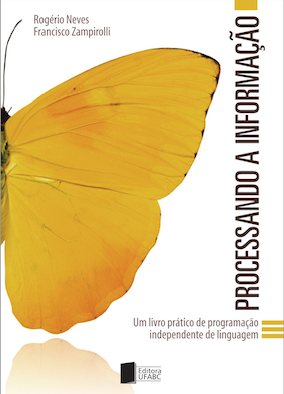
\includegraphics{"figs/Capa_Processando_Informacao.jpg"}

Este caderno (Notebook) é parte complementar \emph{online} do livro
\textbf{\href{https://editora.ufabc.edu.br/matematica-e-ciencias-da-computacao/58-processando-a-informacao}{Processando
a Informação}: um livro prático de programação independente de
linguagem}, que deve ser consultado no caso de dúvidas sobre os temas
apresentados.

\begin{quote}
Este conteúdo pode ser copiado e alterado livremente e foi inspirado
nesse livro.
\end{quote}

    \hypertarget{exercuxedcios}{%
\subsubsection{Exercícios}\label{exercuxedcios}}

    \begin{center}\rule{0.5\linewidth}{0.5pt}\end{center}

\begin{enumerate}
\def\labelenumi{\arabic{enumi}.}
\tightlist
\item
  Criar uma matriz para armazenar as \texttt{C} notas de uma turma e
  calcular a média de cada aluno, considerando uma turma com \texttt{L}
  alunos.
\end{enumerate}

    \begin{center}\rule{0.5\linewidth}{0.5pt}\end{center}

\begin{enumerate}
\def\labelenumi{\arabic{enumi}.}
\setcounter{enumi}{1}
\tightlist
\item
  Em complemento ao exercício anterior, criar também um vetor de String,
  onde para cada posição \texttt{0\textless{}=i\textless{}L} seja
  armazenada a palavra \texttt{"reprovado"} se a nota for abaixo de 5,
  ou \texttt{"aprovado"}, caso contrário.
\end{enumerate}

    \begin{center}\rule{0.5\linewidth}{0.5pt}\end{center}

\begin{enumerate}
\def\labelenumi{\arabic{enumi}.}
\setcounter{enumi}{2}
\tightlist
\item
  Criar uma matriz para armazenar \texttt{L} linhas e \texttt{C}
  colunas. Calcular e exibir a soma dos elementos da diagonal principal
  e secundária da matriz.
\end{enumerate}

    \begin{center}\rule{0.5\linewidth}{0.5pt}\end{center}

\begin{enumerate}
\def\labelenumi{\arabic{enumi}.}
\setcounter{enumi}{3}
\tightlist
\item
  Criar uma matriz para armazenar \texttt{L} linhas e \texttt{C}
  colunas. Calcular a soma dos elementos acima da diagonal da matriz.
\end{enumerate}

    \begin{center}\rule{0.5\linewidth}{0.5pt}\end{center}

\begin{enumerate}
\def\labelenumi{\arabic{enumi}.}
\setcounter{enumi}{4}
\tightlist
\item
  Criar uma matriz \texttt{m1} para armazenar \texttt{L} linhas e
  \texttt{C} colunas. Criar uma outra matriz \texttt{m2} para armazenar
  \texttt{m1} transposta, com \texttt{C} linhas e \texttt{L} colunas,
  sendo que a primeira linha de \texttt{m2} contenha os elementos da
  primeira coluna de \texttt{m1}. Isso se repete para as demais linhas
  de \texttt{m2} e colunas de \texttt{m1}.
\end{enumerate}

    \hypertarget{processando-a-informauxe7uxe3o-cap.-6-matrizes---pruxe1tica-2}{%
\subsection{Processando a Informação: Cap. 6: Matrizes - Prática
2}\label{processando-a-informauxe7uxe3o-cap.-6-matrizes---pruxe1tica-2}}

    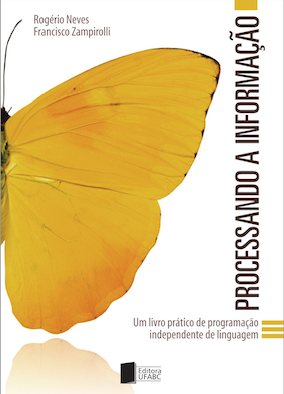
\includegraphics{"figs/Capa_Processando_Informacao.jpg"}

Este caderno (Notebook) é parte complementar \emph{online} do livro
\textbf{\href{https://editora.ufabc.edu.br/matematica-e-ciencias-da-computacao/58-processando-a-informacao}{Processando
a Informação}: um livro prático de programação independente de
linguagem}, que deve ser consultado no caso de dúvidas sobre os temas
apresentados.

\begin{quote}
Este conteúdo pode ser copiado e alterado livremente e foi inspirado
nesse livro.
\end{quote}

    \hypertarget{exercuxedcios}{%
\subsubsection{Exercícios}\label{exercuxedcios}}

    \begin{center}\rule{0.5\linewidth}{0.5pt}\end{center}

\begin{enumerate}
\def\labelenumi{\arabic{enumi}.}
\tightlist
\item
  Criar uma função/método para calcular e retornar o determinante de uma
  matriz \texttt{3\ x\ 3} de valores reais recebida como parâmetro.
\end{enumerate}

    \begin{center}\rule{0.5\linewidth}{0.5pt}\end{center}

\begin{enumerate}
\def\labelenumi{\arabic{enumi}.}
\setcounter{enumi}{1}
\tightlist
\item
  Criar um método que receba uma matriz qualquer de inteiros e imprima
  na tela o valor máximo e o valor mínimo encontrados (não retornando
  nada).
\end{enumerate}

    \begin{center}\rule{0.5\linewidth}{0.5pt}\end{center}

\begin{enumerate}
\def\labelenumi{\arabic{enumi}.}
\setcounter{enumi}{2}
\tightlist
\item
  Criar um método que receba uma matriz de inteiros de qualquer dimensão
  e retorne um vetor contendo a somatória dos valores contidos nas
  colunas.
\end{enumerate}

    \begin{center}\rule{0.5\linewidth}{0.5pt}\end{center}

4.Considere:

\begin{itemize}
\item
  \begin{enumerate}
  \def\labelenumi{\alph{enumi})}
  \tightlist
  \item
    Criar um método que receba uma matriz \texttt{m1} de inteiros
    positivos com \texttt{L} linhas e \texttt{C} colunas e retorne uma
    matriz \texttt{m2}, de mesma dimensão, onde em cada posição
    \texttt{{[}i,j{]}} seja atribuído o cálculo dos máximos entre o
    elemento de \texttt{m1} e seus oito vizinhos:
  \end{enumerate}
\end{itemize}

\begin{longtable}[]{@{}ccc@{}}
\toprule
& vizinhança &\tabularnewline
\midrule
\endhead
\texttt{{[}i-1,j-1{]}} & \texttt{{[}i-1,j{]}} &
\texttt{{[}i-1,j+1{]}}\tabularnewline
\texttt{{[}i\ \ ,j-1{]}} & \textbf{\texttt{{[}i\ ,j{]}}} &
\texttt{{[}i\ \ ,j+1{]}}\tabularnewline
\texttt{{[}i+1,j-1{]}} & \texttt{{[}i+1,j{]}} &
\texttt{{[}i+1,j+1{]}}\tabularnewline
\bottomrule
\end{longtable}

\begin{itemize}
\item
  \begin{enumerate}
  \def\labelenumi{\alph{enumi})}
  \setcounter{enumi}{1}
  \tightlist
  \item
    Generalize este código para os \texttt{m} vizinhos da \texttt{m1} à
    esquerde e à direita e os n vizinhos acima e abaixo.
  \end{enumerate}
\end{itemize}

    \begin{center}\rule{0.5\linewidth}{0.5pt}\end{center}

\begin{enumerate}
\def\labelenumi{\arabic{enumi}.}
\setcounter{enumi}{4}
\tightlist
\item
  Criar um método que receba duas matrizes de valores reais e retorne à
  multiplicação das duas matrizes.
\end{enumerate}

    \hypertarget{processando-a-informauxe7uxe3o-cap.-6-matrizes---pruxe1tica-3}{%
\subsection{Processando a Informação: Cap. 6: Matrizes - Prática
3}\label{processando-a-informauxe7uxe3o-cap.-6-matrizes---pruxe1tica-3}}

    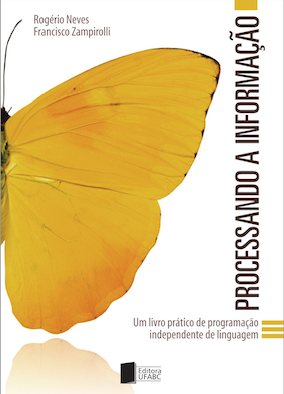
\includegraphics{"figs/Capa_Processando_Informacao.jpg"}

Este caderno (Notebook) é parte complementar \emph{online} do livro
\textbf{\href{https://editora.ufabc.edu.br/matematica-e-ciencias-da-computacao/58-processando-a-informacao}{Processando
a Informação}: um livro prático de programação independente de
linguagem}, que deve ser consultado no caso de dúvidas sobre os temas
apresentados.

\begin{quote}
Este conteúdo pode ser copiado e alterado livremente e foi inspirado
nesse livro.
\end{quote}

    \hypertarget{exercuxedcios}{%
\subsubsection{Exercícios}\label{exercuxedcios}}

Fonte:
\href{http://www.deinf.ufma.br/~csalles/prog/prog_lista2.pdf}{ref1};
\href{http://www.facom.ufu.br/~backes/wordpress/ListaC04.pdf}{ref2}

    \begin{center}\rule{0.5\linewidth}{0.5pt}\end{center}

\begin{enumerate}
\def\labelenumi{\arabic{enumi}.}
\tightlist
\item
  Uma matriz quadrada NxN lógica representa as posições minadas de um
  jogo. Quando uma posição possui o valor VERDADEIRO significa que há
  uma mina ali. Escreva um programa que informa se é possível percorrer
  o tabuleiro de um lado ao outro em linha reta (atravessando uma linha
  inteira ou coluna inteira) ou diagonal sem passar por uma mina sequer.
\end{enumerate}

    \begin{center}\rule{0.5\linewidth}{0.5pt}\end{center}

\begin{enumerate}
\def\labelenumi{\arabic{enumi}.}
\setcounter{enumi}{1}
\tightlist
\item
  Uma imagem em níveis de cinza pode ser representada por uma matriz.
  Leia uma imagem A de números inteiros. Leia também um limiar inteiro.
  Fazer um método para calcular e retornar uma imagem binária de saída B
  com as mesmas dimensões de A, considerando para cada pixel
  A(i,j)\textgreater limear, B(i,j) deve receber o valor 1, caso
  contrário recebe o valor 0. Imprimir as imagens de entrada e saída.
\end{enumerate}

    \begin{center}\rule{0.5\linewidth}{0.5pt}\end{center}

\begin{enumerate}
\def\labelenumi{\arabic{enumi}.}
\setcounter{enumi}{2}
\tightlist
\item
  Leia uma matriz A de inteiros. Criar uma matriz B considerando que
  cada elemento de B é o resultado do elemento de A multiplicado pela
  média dos elementos da linha deste elemento. Arredondar cada elemento
  com o comando \texttt{round}.
\end{enumerate}

    \begin{center}\rule{0.5\linewidth}{0.5pt}\end{center}

\begin{enumerate}
\def\labelenumi{\arabic{enumi}.}
\setcounter{enumi}{3}
\tightlist
\item
  Faça um programa para gerar automaticamente números entre 0 e 99 de
  uma cartela de bingo. Sabendo que cada cartela deverá conter 5 linhas
  de 5 números, gere estes dados de modo a não ter números repetidos
  dentro das cartelas. O programa deve exibir na tela a cartela gerada.
\end{enumerate}

    \begin{center}\rule{0.5\linewidth}{0.5pt}\end{center}

\begin{enumerate}
\def\labelenumi{\arabic{enumi}.}
\setcounter{enumi}{4}
\tightlist
\item
  Leia uma matriz 5 x 10 que se refere respostas de 10 questõs de
  múltipla escolha, referentes a 50 candidatos de um processo seletivo.
  Leia também um vetor de 10 posições contendo o gabarito de respostas
  que podem ser a, b, c, d ou e. Seu programa deverá comparar as
  respostas de cada candidato com o gabarito e emitir um vetor
  denominado resultado, contendo a pontuação correspondente a cada
  candidato. Imprimir também a lista de aprovados e em seguinda a lista
  de reprovados, considernado média 5.
\end{enumerate}

    \begin{center}\rule{0.5\linewidth}{0.5pt}\end{center}

\begin{enumerate}
\def\labelenumi{\arabic{enumi}.}
\setcounter{enumi}{5}
\tightlist
\item
  Leia uma matriz A de inteiros. Qual é o maior produto de quatro
  números adjacentes em qualquer direção (cima, baixo, esquerda,
  direita, ou nas diagonais) na matriz de 20x20 e em qual(is)
  coordenada(s) ocorreu(ram)? Ou seja, em cada posição
  \texttt{{[}i,j{]}} de A cálcular o máximo valor entre as
  multiplicações dos elementos abaixo:
\end{enumerate}

\begin{longtable}[]{@{}ccc@{}}
\toprule
& vizinhança &\tabularnewline
\midrule
\endhead
\texttt{{[}i-1,j-1{]}} & \texttt{{[}i-1,j{]}} &
\texttt{{[}i-1,j+1{]}}\tabularnewline
\texttt{{[}i\ \ ,j-1{]}} & \textbf{\texttt{{[}i\ ,j{]}}} &
\texttt{{[}i\ \ ,j+1{]}}\tabularnewline
\texttt{{[}i+1,j-1{]}} & \texttt{{[}i+1,j{]}} &
\texttt{{[}i+1,j+1{]}}\tabularnewline
\bottomrule
\end{longtable}

    \begin{center}\rule{0.5\linewidth}{0.5pt}\end{center}

\begin{enumerate}
\def\labelenumi{\arabic{enumi}.}
\setcounter{enumi}{6}
\tightlist
\item
  Uma matriz de caracteres 3x3 foi utilizada para armazenar uma partida
  de jogo da velha. Os caracteres `O' e `X' foram utilizados para
  armazenar a jogada de cada participante. Informe na tela se o vencedor
  foi o jogador `O', o jogador `X' ou se o resultado foi empate.
  IMPORTANTE: não serão informadas partidas com dois vencedores, apenas
  partidas válidas e todas as 9 casas estarão preenchidas com `O' ou
  `X'.
\end{enumerate}

    \begin{center}\rule{0.5\linewidth}{0.5pt}\end{center}

\begin{enumerate}
\def\labelenumi{\arabic{enumi}.}
\setcounter{enumi}{7}
\tightlist
\item
  Faça um programa para determinar a próxima jogada em um Jogo da Velha.
  Assumir que o tabuleiro é representado por uma matriz de 3 x 3, onde
  cada posição representa uma das casas do tabuleiro. A matriz pode
  conter os seguintes valores -1, 0, 1 representando respectivamente uma
  casa contendo uma peça minha (-1), uma casa vazia do tabuleiro (0), e
  uma casa contendo uma peça do meu oponente (1).
\end{enumerate}

    \hypertarget{processando-a-informauxe7uxe3o-cap.-6-matrizes---pruxe1tica-4}{%
\subsection{Processando a Informação: Cap. 6: Matrizes - Prática
4}\label{processando-a-informauxe7uxe3o-cap.-6-matrizes---pruxe1tica-4}}

    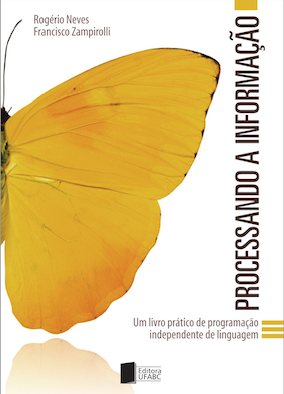
\includegraphics{"figs/Capa_Processando_Informacao.jpg"}

Este caderno (Notebook) é parte complementar \emph{online} do livro
\textbf{\href{https://editora.ufabc.edu.br/matematica-e-ciencias-da-computacao/58-processando-a-informacao}{Processando
a Informação}: um livro prático de programação independente de
linguagem}, que deve ser consultado no caso de dúvidas sobre os temas
apresentados.

\begin{quote}
Este conteúdo pode ser copiado e alterado livremente e foi inspirado
nesse livro.
\end{quote}

    \hypertarget{exercuxedcios}{%
\subsubsection{Exercícios}\label{exercuxedcios}}

    \begin{center}\rule{0.5\linewidth}{0.5pt}\end{center}

EP5\_1 - Média dos alunos

    \hypertarget{ler-uma-matriz-linha-por-linha}{%
\paragraph{Ler uma matriz LINHA por
LINHA:}\label{ler-uma-matriz-linha-por-linha}}

    \hypertarget{ler-uma-matriz-considerando-cada-elemento-da-matriz-uma-entrada}{%
\paragraph{Ler uma matriz considerando cada ELEMENTO da matriz uma
entrada:}\label{ler-uma-matriz-considerando-cada-elemento-da-matriz-uma-entrada}}


    % Add a bibliography block to the postdoc
    
    
    
\end{document}
